\documentclass[12pt]{book}
\usepackage[portuguese]{babel}
\usepackage{graphicx}
\usepackage{indentfirst}
\usepackage[utf8]{inputenc}
\usepackage{amssymb}
\usepackage{enumitem}
\usepackage{color}
\usepackage[fleqn]{amsmath}
\usepackage[a4paper, margin=1.0in]{geometry}
\usepackage{verbatim}

% INICIO CONFIGURACAO DO HYPER LINK %
\usepackage{hyperref}
\usepackage[dvipsnames]{xcolor}
\newcommand\myshade{85}
\colorlet{mylinkcolor}{violet}

\hypersetup{
	linkcolor  = mylinkcolor!\myshade!black,
	citecolor  = mylinkcolor!\myshade!black,
	urlcolor   = mylinkcolor!\myshade!black,
	colorlinks = true,
}
% FIM CONFIGURACAO DO HYPER LINK %

\usepackage{amsthm, amssymb, amsfonts, amsmath}
\usepackage{graphicx}
\usepackage{tikz}
\usetikzlibrary{calc,shapes}
\usepackage{mathtools}
\usepackage{mathrsfs}
\usepackage{tikz-cd}

% PACOTES PARA DIAGRAMAS %
\usepackage[all,cmtip]{xy}
% PACOTES PARA DIAGRAMAS %

% QUALIFICADORES DOS RESULTADOS: TEOREMAS, LEMAS, COROLARIOS E PROVA %
\newtheorem{teorema}{Teorema}[section]
\newtheorem{corolario}[teorema]{Corolário}
\newtheorem{convensao}[teorema]{Convensão}
\newtheorem{lema}[teorema]{Lema}
\newtheorem{definicao}[teorema]{Definição}
\newtheorem{exemplo}[teorema]{Exemplo}
\newtheorem{observacao}[teorema]{Observação}
\newtheorem{proposicao}[teorema]{Proposição}
\newenvironment{prova}[1]{$\square$ #1}{\hfill$\blacksquare$}
% QUALIFICADORES DOS RESULTADOS: TEOREMAS, LEMAS, COROLARIOS E PROVA %

% AQUI ESTAO OS COMANDOS %
\newcommand{\aplicacaoexponencial}[2]{\exp_{#1}(#2)}
\newcommand{\aplicacaoexponencialgeral}[1]{exp_{#1}}
\newcommand{\aplicaoessuaves}[2]{C^{\infty}(#1, #2)}
\newcommand{\aplicaoessuavesloc}[2]{C^{\infty}_{\text{loc}}(#1, #2)}
\newcommand{\aplicaoessuavesreatacirculo}{C^{\infty}(\retacartesianocirculo; M)}
\newcommand{\autoespaco}[1]{E_{#1}}
\newcommand{\bigmodulo}[1]{\Bigm\lvert #1 \Bigm\lvert }
\newcommand{\bigparenteses}[1]{\Big( #1 \Big) }
\newcommand{\bordo}[1]{\partial_{#1}}
\newcommand{\bordorel}[1]{\overline{\partial}_{#1}}
\newcommand{\cadeia}[2]{C_{#1}(#2; A)}
\newcommand{\caminhosfechadoscirculo}[2]{L([#1,#2], S^{1})}
\newcommand{\caminhosfechadospontobase}[2]{\mathcal{L}^{o}_{#1}(#2)}
\newcommand{\caminhosfechadosSp}[2]{L([#1,#2], \gruposimpletico{2n})}
\newcommand{\caminhosespeciais}[1]{\mathcal{L}^{*}(#1)}
\newcommand{\caminhosdecaimentoexponencial}[2]{C^{\infty}_{\searrow}(#1, #2)}
\newcommand{\caminhosdecaimentoexponencialpadrao}{\caminhosdecaimentoexponencial{x^{-}}{x^{+}}}
\newcommand{\caminhosexponenciaisconectantesabrev}{\mathcal{P}}
\newcommand{\caminhosexponenciaisconectantes}[2]{\mathcal{P}^{1,p}(#1, #2)}
\newcommand{\caminhosexponenciaisSobolev}{\mathcal{L}^{1,p}M}
\newcommand{\caminhosexponenciaisconectantespadrao}{\caminhosexponenciaisconectantes{x^{-}}{x^{+}}}
\newcommand{\caminhos}{\mathcal{L}}
\newcommand{\caminhosfechados}[1]{\caminhos^{o}(#1)}
\newcommand{\caminhoslagrangianos}[3]{\caminhos_{#3}(#1,#2)}
\newcommand{\caminhoslagrangianosV}[2]{\caminhoslagrangianos{#1}{#2}{V}}
\newcommand{\caminhospontobase}[1]{\caminhos_{#1}}
\newcommand{\caminhossempontobase}[1]{\caminhos(#1)}
\newcommand{\caminhosNaoDegeneradosSp}{\caminhos^{*}(\gruposimpletico{2n})}
\newcommand{\caminhospontobasegeral}[2]{\caminhos_{#1}(#2)}
\newcommand{\caminhossuavesconectantes}[2]{\caminhos(#1, #2)}
\newcommand{\caminhossubespacoslagrangianos}[2]{L[#1,#2]}
\newcommand{\campogradiente}{\mathcal{X}}
\newcommand{\campogradientefuncional}{\mathcal{X}_{\mathcal{A}}}
\newcommand{\campohamiltoniano}[1]{X_{H}(#1)}
\newcommand{\campohamiltonianoabrev}{X_{H}}
\newcommand{\campossuaves}[1]{\mathfrak{X}(#1)}
\newcommand{\celula}[2]{D^{#1}_{#2}}
\newcommand{\celulabordo}[2]{\partial D^{#1}_{#2}}
\newcommand{\circulo}{S^{1}}
\newcommand{\circulovariedade}{\circulo\times M}
\newcommand{\cktopologia}[1]{\mathcal{C}^{#1}\text{-topologia}}
\newcommand{\classe}[1]{[#1]}
\newcommand{\cohomologia}[2]{H^{#1}(#2)}
\newcommand{\cohomologiadual}[2]{H^{#1}(#2)^{*}}
\newcommand{\cohomologiacompac}[2]{H^{#1}_{c}(#2)}
\newcommand{\cohomologiacompacdual}[2]{H^{#1}_{c}(#2)^{*}}
\newcommand{\colecao}[1]{\{#1_{k} \}_{k\in \inteiros}}
\newcommand{\colecaoabrev}[1]{\{#1 \}_{k\in \inteiros}}
\newcommand{\colecaofinita}[2]{\{#1_{j} \}_{j=1}^{#2}}
\newcommand{\colecaofinitaabrev}[2]{\{#1 \}_{j=1}^{#2}}
\newcommand{\complementar}[2]{#1 \backslash #2}
\newcommand{\complexificacao}[1]{#1_{\complexo{}}}
\newcommand{\complexificacaotensorial}[1]{\complexo{}\otimes_{\reta} #1}
\newcommand{\complexificado}[1]{\mathcal{#1}}
\newcommand{\complexificacaoelemento}[2]{#1\otimes_{\reta} #2}
\newcommand{\complexo}[1]{\mathbb{C}^{#1}}
\newcommand{\coordenada}[2]{#1_{(#2)}}
\newcommand{\diferencialfloer}{D\operadorFloer}
\newcommand{\diferencialfloerponto}[1]{D_{#1}\operadorFloer}
\newcommand{\diferencialfloerabrev}{\mathcal{D}}
\newcommand{\derivada}[2]{\frac{d #1}{d #2}}
\newcommand{\derivadaparcial}[2]{\frac{\partial #1}{\partial #2}}
\newcommand{\derivadaparcialdois}[2]{\frac{\partial^{2} #1}{\partial #2^{2}}}
\newcommand{\derivadaparcialdoisdois}[3]{\frac{\partial^{2} #1}{\partial #2 \partial#3}}
\newcommand{\derivadaparcialabrev}[1]{\partial_{#1}}
\newcommand{\diag}{\text{diag}}
\newcommand{\diferencialhamiltoniano}[1]{(dX_{H})_{#1}}
\newcommand{\distribuicoes}{\distribuicoesgeral{\Omega}}
\newcommand{\distribuicoesgeral}[1]{\mathcal{D'}(#1)}
\newcommand{\dominioMaslov}{\caminhos^{*}(\gruposimpletico{2n})}
\newcommand{\energiafinitaM}{\mathcal{M}}
\newcommand{\energiafinitaMHamiltoniana}[1]{\energiafinitaM(#1, J)}
\newcommand{\energiafinitaMconectante}{\energiafinitaM(x^{-}, x^{+})}
\newcommand{\energiafinitaMconectanteHamiltoniana}{\energiafinitaM(x^{-}, x^{+},H+h,J)}
\newcommand{\espacoLdois}[1]{L^{2}(#1)}
\newcommand{\espacoLp}[1]{L^{p}(#1)}
\newcommand{\espacoLpcomp}[1]{L^{p}_{loc}(#1)}
\newcommand{\espacoLpcontradominio}[2]{L^{p}(#1;#2)}
\newcommand{\espacoLpGeral}[2]{L^{#1}(#2)}
\newcommand{\espacoLpretacirculo}{\espacoLpcontradominio{\retacartesianocirculo}{\real{2n}}}
\newcommand{\espacoLpadjuntoretacirculo}{L^{q}(\retacartesianocirculo;\real{2n})}
\newcommand{\espacoLpdual}{(L^{p})^{*}(\retacartesianocirculo;\real{2n})}
\newcommand{\espacomoduli}[2]{\mathcal{M}_{#1#2}}
\newcommand{\espacoSimpleticoOrtogonal}[1]{#1^{\omega}}
\newcommand{\espacosobolev}[1]{W^{1,p}(#1)}
\newcommand{\espacosobolevcontradominio}[2]{W^{1,p}(#1;#2)}
\newcommand{\espacosobolevadjuntoretacirculo}{W^{1,q}(\retacartesianocirculo;\real{2n})}
\newcommand{\espacosobolevdual}{(W^{1,p})^{*}(\retacartesianocirculo;\real{2n})}
\newcommand{\espacosobolevgeneralizadocontra}[2]{W^{k,p}(#1; #2)}
\newcommand{\espacosobolevgeneralizado}[1]{W^{k,p}(#1)}
\newcommand{\espacosobolevretacirculo}{\espacosobolevcontradominio{\retacartesianocirculo}{\real{2n}}}
\newcommand{\espacosobolevdois}[2]{\espacosobolevgeral{2}{#1, #2}}
\newcommand{\espacosobolevgeral}[2]{W^{1,#1}(#2)}
\newcommand{\espacotangente}[1]{\espacotangenteponto{p}{#1}}
\newcommand{\espacotangentevariedadeestavel}{T^{s}_{p}M}
\newcommand{\espacotangentevariedadeinstavel}{T^{u}_{p}M}
\newcommand{\espacotangenteponto}[2]{T_{#1}#2}
\newcommand{\espacotangentevariedade}{\espacotangenteponto{p}{M}}
\newcommand{\espectrooperador}[1]{\sigma(#1)}
\newcommand{\estruturacomplexa}{J_{0}}
\newcommand{\estruturascomplexas}[2]{\mathcal{J}(#1, #2)}
\newcommand{\estruturascomplexasM}{\mathcal{J}(M)}
\newcommand{\estruturascomplexaspadrao}{\mathcal{J}(V, \omega)}
\newcommand{\Exp}{\text{Exp}}
\newcommand{\fibradocaminhosexponenciais}{\mathcal{E}(x^{-}, x^{+})}
\newcommand{\fibradocaminhosexponenciaisabrev}{\mathcal{E}}
\newcommand{\formaSimpletica}[2]{\omega(#1, #2)}
\newcommand{\formaSimpleticaabrev}{\omega_{0}}
\newcommand{\formaSimpleticaExtendida}[2]{\Omega(#1, #2)}
\newcommand{\formaSimpleticaPadrao}[2]{\omega_{0}(#1, #2)}
\newcommand{\funcaocond}[5]{
	#1 = 
	\left\{
	\begin{array}{cc}
		#2, & #3\\
		#4, & #5\\
	\end{array}
	\right.
}
\newcommand{\funcionalH}{\mathcal{A}_{H}}
\newcommand{\funcionalHponto}[1]{\mathcal{A}_{H}(#1)}
\newcommand{\funcoesdiferenciaveis}[2]{C^{#1}(#2)}
\newcommand{\funcoesdiferenciaveissupp}[2]{C^{#1}_{c}(#2)}
\newcommand{\funcoesmorse}[1]{\mathcal{M}_{o}(#1)}
\newcommand{\funcoesmorsesmale}[1]{\mathcal{M}^{S}_{o}(#1)}
\newcommand{\funcoessuaves}[1]{C^{\infty}(#1, \real{})}
\newcommand{\funcoesteste}{\funcoestestegeral{\Omega}}
\newcommand{\funcoestestegeral}[1]{\mathcal{D}(#1)}
\newcommand{\generalgroup}[2]{GL(#1, #2)}
\newcommand{\generalgroupreal}[1]{\generalgroup{#1}{\real{}}}
\newcommand{\generalgroupcomplexo}[1]{\generalgroup{#1}{\complexo{}}}
\newcommand{\gerador}[1]{\langle #1\rangle}
\newcommand{\gradiente}{\nabla f}
\newcommand{\gradientefuncional}{\nabla \funcionalH}
\newcommand{\grupofundamental}[1]{\pi_{1}(#1)}
\newcommand{\grupofundamentalpontobase}[2]{\pi_{1}(#1; #2)}
\newcommand{\gruposimpletico}[1]{Sp(#1)}
\newcommand{\gruposimpleticocomplexo}[1]{Sp(#1; \complexo{})}
\newcommand{\gruposimpleticoreal}[1]{Sp(#1;\reta)}
\newcommand{\gruposimpleticoespecial}[1]{Sp^{1}(#1)}
\newcommand{\gruposimpleticonaodegenerado}[1]{Sp^{#1}(2n)}
\newcommand{\gruposimpleticopositivo}[1]{Sp_{+}(#1)}
\newcommand{\hamiltonianasRegulares}{\mathcal{H}_{reg}}
\newcommand{\hessianaponto}[2]{\text{Hess}_{#1}(#2)}
\newcommand{\homologia}[2]{H_{#1}(#2;A)}
\newcommand{\homologiaabrev}[2]{H_{#1}(#2)}
\newcommand{\homologiarel}[3]{H_{#1}(#2,#3)}
\newcommand{\homologiarelcel}[3]{H_{#1}(D^{#2}_{#3}, \partial D^{#2}_{#3})}
\newcommand{\homologiarelskele}[3]{H_{#1}(X^{(#2)}, X^{(#3)})}
\newcommand{\homologiarelskelesimpl}[2]{H_{#1}(X^{(#2)}, X^{(#2-1)})}
\newcommand{\iconley}[1]{\iconleyabrev(#1)}
\newcommand{\iconleyabrev}{\mu_{CZ}}
\newcommand{\imagembordo}[2]{B_{#1}(#2;A)}
\newcommand{\imagembordoabrev}[2]{B_{#1}(#2)}
\newcommand{\ind}{\text{Ind}}
\newcommand{\induzida}[1]{#1_{\#}}
\newcommand{\inteiros}{\mathbb{Z}}
\newcommand{\inteirospos}{\inteiros_{+}}
\newcommand{\iprod}[2]{\langle #1, #2 \rangle}
\newcommand{\intervalo}{[0,1]}
\newcommand{\intervalofechado}[1]{[-#1,#1]}
\newcommand{\kernelbordo}[2]{Z_{#1}(#2;A)}
\newcommand{\kernelbordoabrev}[2]{Z_{#1}(#2)}
\newcommand{\liederivada}[1]{\mathcal{L}_{#1}}
\newcommand{\operadoreslimitadosauto}[1]{\mathcal{B}(#1)}
\newcommand{\operadorFloer}{\mathcal{F}}
\newcommand{\operadorFloerDefinicao}[1]{\derivadaparcial{#1}{s} + J(#1)\derivadaparcial{#1}{t} - J(#1)X_{H}(#1)}
\newcommand{\operadorFloerParametro}[1]{\mathcal{F}(#1)}
\newcommand{\operadorFloerPadrao}{\operadorFloerParametro{u}}
\newcommand{\matrizantisimetrica}[1]{Asym(#1)}
\newcommand{\matrizortogonal}[1]{O(#1)}
\newcommand{\matrizquadcomplexa}[1]{M_{#1 \times #1}(\complexo{})}
\newcommand{\matrizquadreal}[1]{M_{#1 \times #1}(\real{})}
\newcommand{\matrizsimetrica}[1]{Sym(#1)}
\newcommand{\matrizSimpleticaOrtogonal}{\mathcal{U}}
\newcommand{\matrizsimetricapositiva}[1]{Sym_{+}(#1)}
\newcommand{\matrizsimpleticapositiva}[1]{Sp_{+}(#1)}
\newcommand{\matrizunitaria}[1]{U(#1)}
\newcommand{\norma}[1]{||#1||}
\newcommand{\normagrande}[1]{\Big|\Big|#1\Big|\Big|}
\newcommand{\normaLdois}[1]{||#1||_{L^{2}}}
\newcommand{\normaLp}[1]{||#1||_{L^{p}}}
\newcommand{\normaLpdefinicao}[2]{ \Big(\int_{#2}#1^{p}\Big)^{1/p}}
\newcommand{\normaLpDominio}[2]{||#1||_{L^{p}(#2)}}
\newcommand{\normaLgGeral}[3]{\norma{#1}_{\espacoLpGeral{#2}{#3}}}
\newcommand{\normapequenaLpdefinicao}[2]{ \normaLpdefinicao{\norma{#1}}{#2}}
\newcommand{\normagrandeLpdefinicao}[2]{ \normaLpdefinicao{\normagrande{#1}}{#2}}
\newcommand{\normasubscrito}[2]{\norma{#1}_{#2}}
\newcommand{\normaWp}[1]{||#1||_{W^{1,p}}}
\newcommand{\normaWpgeneralizado}[1]{||#1||_{W^{k,p}}}
\newcommand{\normaWpgeral}[2]{||#1||_{W^{1,#2}}}
\newcommand{\normaWpGeralDominio}[3]{\norma{#1}_{W^{1,#2}(#3)}}
\newcommand{\normaWpDominio}[2]{||#1||_{W^{1,p}(#2)}}
\newcommand{\operadorcauchyabrev}[1]{\overline{\partial}_{#1}}
\newcommand{\operadoresfredholm}[2]{\mathcal{F}r(#1, #2)}
\newcommand{\operadoreslimitados}[2]{\mathcal{B}(#1, #2)}
\newcommand{\orbitaponto}[1]{\mathcal{O}(#1)}
\newcommand{\orbitasconectantes}[2]{\mathcal{M}(#1, #2)}
\newcommand{\orbitasConectantesZ}{\mathcal{Z}(x^{-}, x^{+},H, J)}
\newcommand{\orbitasconectantespadrao}{\mathcal{M}(x^{-}, x^{+})}
\newcommand{\paresregulares}{\mathcal{H}_{reg}}
\newcommand{\parteImaginaria}[1]{\Im(#1)}
\newcommand{\parteReal}[1]{\Re(#1)}
\newcommand{\perturbacaoHamiltoniana}[1]{C^{\infty}_{\epsilon}(#1)}
\newcommand{\pontoscriticos}[1]{\textit{Cr}(#1)}
\newcommand{\pontoscriticosordem}[2]{\textit{Cr}^{(#1)}(#2)}
\newcommand{\produtointerno}[2]{\langle #1, #2 \rangle}
\newcommand{\produtointernoabrev}{\langle ., .\rangle}
\newcommand{\produtosinternos}[1]{Riem(#1)}
\newcommand{\produtotensorial}[2]{ #1_{1} \otimes_{\mathbb{K}} \dots \otimes_{\mathbb{K}} #1_{#2}}
\newcommand{\produtotensorialabrev}[2]{#1\otimes #2}
\newcommand{\produtotensorialdual}{\produtotensorialabrev{\complexificado{V}^{*}}{\complexificado{V}^{*}}}
\newcommand{\produtotensorialreal}[2]{\bigotimes_{j=1}^{#1} #2_{j}}
\newcommand{\pullbackfibradotangente}[2]{#1^{*}T#2}
\newcommand{\pullbackfibradotangenteM}[1]{\pullbackfibradotangente{#1}{M}}
\newcommand{\pullbackfibradotangenteMpadrao}{\pullbackfibradotangente{u}{M}}
\newcommand{\retacartesianocirculo}{\real{} \times \circulo}
\newcommand{\retacartesianovariedade}{\real{} \times M}
\newcommand{\real}[1]{\mathbb{R}^{#1}}
\newcommand{\realprojetivo}[1]{\mathbb{R}P^{#1}}
\newcommand{\reta}{\real{}}
\newcommand{\subespacoslagrangianos}{L(V)}
\newcommand{\lacocontrateis}{\mathcal{L}^{o}M}
\newcommand{\somadir}[1]{\bigoplus \limits_{#1}}
\newcommand{\cilindrosLM}{\mathcal{C}M}
\newcommand{\morsefunc}[1]{\mathcal{M}o(#1)}
\newcommand{\skeleton}[1]{X^{(#1)}}
\newcommand{\variedadeconectante}{\variedadeconectantepontos{p}{q}}
\newcommand{\variedadeconectantepontos}[2]{W_{#1#2}}
\newcommand{\variedadeestavel}[1]{W^{s}(#1)}
\newcommand{\variedadeinstavel}[1]{W^{u}(#1)}
\newcommand{\aviso}[1]{{\color{violet}(#1)}}
\newcommand{\alerta}[1]{{\color{red}#1}}
% AQUI ESTAO OS COMANDOS %

\begin{document}
	
	\title{O Índice de Maslov e suas Aplicações em Topologia Simplética: a homologia de Floer e a Conjectura de Arnold.}
	
	\author{Vinicius Fernandes}
	
	\maketitle
	
	\tableofcontents
	
	\chapter*{Introdução}\label{capitulo_introducao}
	Como muitas das construções desenvolvidas na matemática a Homologia de Floer teve como motivação um problema de origem na Física, mais especificamente, no estudo de sistemas Hamiltonianos. A descrição Newtoniana da mecânica clássica tem como um de seus equivalentes a descrição Hamiltoniana. Nesse contexto, grande parte dos sistemas dinâmicos Hamiltonianos podem ser desenvolvidos em uma 2n-variedade diferenciável $M$ munida de uma 2-forma fechada e não degenerada $\omega$. O sistema dinâmico é modelado por uma função Hamiltoniana dependente do tempo $H: M\times \reta\to \reta$ satisfazendo a equação geométrica $\omega_{x}(\campohamiltonianoabrev(x,t), Y) = d_{x}H(Y)$ para todo $Y \in \espacotangenteponto{x}{M}$ e todo $x \in M$, onde o campo vetorial $\campohamiltonianoabrev \in \campossuaves{M}$ é chamado de campo Hamiltoniano associado a $H$. O sistema de equações diferenciais $\dot{x} = \campohamiltoniano{(x,t)}$ é chamado sistema Hamiltoniano e suas soluções dão origem a uma família de difeomorfismos $\psi_{t}:M\to M$, onde $t\in \reta$, que satisfaz a equação diferencial
	$$
	\dot{\psi}_{t}(x) = \campohamiltoniano{\psi_{t}(x),t}.
	$$
	
	Sejam $(M, \omega )$ uma 2n-variedade simplética e $\psi:M \to M$ um difeomorfismo tal que $\psi^{*}\omega = \omega$. Então $\psi$ é chamado de simplectomorfismo. Pode-se mostrar que $\psi_{t}:M\to M$ é um simplectomorfismo e o conjunto $G=\{\psi_{t}: t \in \reta\}$ forma um grupo de difeomorfismos com a operação de composição, chamado grupo de aplicações Hamiltonianas (ou grupo a 1-parâmetro de difeomorfismos).
	
	Foi estudando sistemas dinâmicos Hamiltonianos que V. I. Arnold formulou a primeira versão da conjectura que atualmente leva seu nome. De acordo com a Teoria de Lefschetz toda aplicação Hamiltoniana possui ao menos um ponto fixo, quando a característica de Euler de $M$ é não-nula. A ideia de Arnold era generalizar esse resultado, o que levou a seguinte versão da conjectura:
	
	\textbf{Conjectura de Arnold (V1):} \textit{Seja $\phi$ uma aplicação Hamiltoniana em uma 2n-variedade compacta simplética $(M, \omega)$. Então, o número de pontos fixos de $\phi$ é, no mínimo, o número de pontos críticos de uma função Hamiltoniana em $M$.}
	
	Posteriormente, trabalhando em particularizações do problema, tais como $T^{2}$ e $S^{2}$, Arnold observou que, se a função Hamiltoniana $H$ depende periodicamente no tempo, isto é, $H:\circulovariedade\to \reta$ tem período 1, então as soluções 1-periódicas do campo Hamiltoniano estão em bijeção com os pontos fixos da função Hamiltoniana. Com isso, ao invés de determinar diretamente os pontos fixos da aplicação Hamiltoniana $\phi$, basta determinar as soluções 1-periódicas do sistema Hamiltoniano. O que resultou na seguinte reformulação da conjectura
	
	\textbf{Conjectura de Arnold (V2):} \textit	{Seja $(M,\omega)$ uma 2n-variedade compacta e simplética. Defina $H:M\times \real{} \to \reta$ uma função Hamiltoniana 1-periódica e suponha que as soluções 1-periódicas do sistema Hamiltoniano sejam não-degeneradas. Então o número de soluções $\mathcal{N}$ desse sistema será limitado inferiormente pela soma dos números de Betti de M, isto é:
		$$
		\mathcal{N}\geq \sum_{i=0}^{2n}\beta_{i}(M),
		$$
		onde $\beta_{i}(M)$ é a dimensão do i-ésimo grupo de homologia singular de $M$.}
	
	Motivado pela demonstração dessa conjectura, nasce um dos principais formalismos no estudo da topologia simplética: a Homologia de Floer.
	
	O fato de estar presente a soma dos números de Betti na conjectura nos conduz a ideia de construirmos uma homologia que tenha como ingredientes as soluções do sistema Hamiltoniano. Mas uma abordagem similiar já era conhecida: a Homologia de Morse-Witten. Também tem origem em problemas de sistemas dinâmicos da Física, mais espeficicamente, em estudos dos aspectos topológicos de sistemas quânticos por Edward Witten $\cite{witten_supersymmetry_morse}$.
	
	A construção de Witten traz um entendimento geométrico do operador bordo do complexo de cadeias. Munindo a variedade $M$ com uma métrica Riemanniana, determina-se os pontos críticos de função de Morse $f: M \to \reta$ e mostra-se que, para cada par de pontos críticos com índices consecutivos, existe um número finito de linhas do fluxo gradiente conectando-os. O conjunto de tais linhas são subvariedades de $M$ chamadas variedades de conexão. Escolhemos  uma orientação para a variedade de conexão. Witten definiu o grupo das $k$-cadeias como sendo o grupo abeliano gerado pelos pontos críticos com índice de Morse igual a $k$. Já o operador bordo, quando avaliado em uma k-cadeia, é a soma sob todas as $(k-1)$-cadeias, sendo que os coeficientes dessa soma são inteiros cujo sinal esta relacionado com a orientação da variedade de conexão e com a orientação da variedade instável da k-cadeia. Essa é uma metodologia simples e elegante de cálculo da homologia da variedade que permite o estudo dos aspectos topológicos das variedades via sistemas dinâmicos, sendo que a dinâmica é materializada no gradiente da função de Morse $f$.
	
	É tentador nos enveredarmos na demonstração da conjectura de Arnold via construção de Witten. Contudo, dificuldades técnicas fizeram com que uma abordagem ligeiramente diferente fosse realizada por Floer. Em vez de estudar o gradiente de uma função Hamiltoniana definida na variedade $M$ a estratégia foi analisar o comportamento do funcional $\funcionalH$, chamado funcional de ação, definido no espaço de curvas 1-periódicas e contráteis em $M$. Aplicando o princípio variacional clássico, determina-se que as soluções 1-periódicas e contráteis do sistema Hamiltoniano são os pontos críticos do funcional de ação $\pontoscriticos{\funcionalH}$. Essa técnica é conhecido como abdordagem variacional. Uma das grandes dificuldades nesse cenário é que o conjunto de curvas 1-periódicas e contráteis forma uma variedade de dimensão infinita, com isso, estabelecer uma análogo ao índice de Morse para os pontos críticos do funcional é uma tarefa árdua. Foi necessária a construção de um operador de Fredholm e de um índice de Maslov, que generaliza o ideia do índice de Morse para dimensão infinita.
	
	O princípio variacional aplicado no funcional de ação resulta na determinação das solução de um sistema de equações diferenciais parciais de primeira ordem. A esse sistema de equações diferenciais é associado um operador diferencial, chamado operador de Floer, cujas soluções são as curvas integrais que conectam os pontos críticos do funcional de ação, situação análoga a determinação das linhas de fluxo do gradiente negativo.
	
	O operador de Floer é um operador linear e limitado definido no espaço de todas as curvas que conectam um par de pontos críticos do funcional de ação. Mostra-se que esse espaço é uma variedade de dimensão infinita (uma variedade de Banach) e que o diferencial de tal operador é um operador de Fredholm. A todo operador de Fredholm associa-se um número inteiro, chamado índice de Fredholm, que no caso em que estamos interessados, coincide com a diferença dos índices de Maslov de cada um dos pontos críticos. Feito isso, pode-se mostrar que, no caso de uma função Hamiltoniana independente do tempo e cuja Hessiana é limitada, tal índice coincide com o índice de Morse, a menos de uma constante. Tem-se aqui uma generalização da Homologia de Morse-Witten.
	
	Essa generalização é uma consequência da definição do complexo de Floer e sua homologia. Analogamente ao complexo de Morse-Witten, as k-cadeias do complexo de Floer são geradas pelos pontos críticos do funcional de ação $\funcionalH$ de índice $k \in \inteiros_{+}$. A indexação dos pontos críticos do funcional de ação é dada pelo índice de Conley-Zehnder $\iconleyabrev:\pontoscriticos{\funcionalH} \to \inteiros$, e é um dos pontos de maior complexidade do texto, e tal dificuldade se dá pelo fato de que os pontos críticos são caminhos na variedade $M$. Com isso, o k-ésimo operador bordo do complexo é um homomorfismo que tem como imagem uma (k-1)-cadeia gerada pelos pontos críticos do fincional de ação $\funcionalH$ com índice $k-1 \in \inteiros_{+}$.
	
	
	\chapter{Preliminares de Topologia Algébrica}
	A topologia algébrica é o ramo da matemática no qual se utiliza estruturas algébricas para se analisar a topologia de um conjunto (um espaço topológico) e seus invariantes. 
	
	\section{Grupo Fundamental e a Aplicação Grau}\label{capitulo_grupo_fundamental}
	Nessa seção será abordada um caso específico de estrutura algébrica de um espaço topológico $X$, chamado grupo fundamental de $X$. Mais detalhes dos resultados aqui enunciados podem ser encontrados em \cite{elon_grupo_fundamental} e \cite{massey}.
	
	\subsection{Grupo Fundamental}
	
	Sejam $X$ um espaço topológico e $\caminhossempontobase{X}$ o conjunto dos caminhos contínuos $\gamma:[0,1]\to X$. Tome $\gamma, \beta \in \caminhossempontobase{X}$ tais que $\gamma(1) = \beta(0)$. Definimos a justaposição $*:\caminhossempontobase{X}\times \caminhossempontobase{X} \to \caminhossempontobase{X}$ entre $\gamma$ e $\beta$ por
	$$
	\funcaocond{(\gamma*\beta)(t)}{\gamma(2t)}{0\leq t \leq 1/2}{\beta(2t-1)}{1/2 \leq t \leq 1}.
	$$
	
	Dado um caminho $\gamma\in \caminhossempontobase{X}$, seu caminho inverso $\hat{\gamma} \in \caminhossempontobase{X}$ é definido por $\hat{\gamma} (t) = \gamma(1-t)$.
	
	\begin{observacao}
		Quando não houver ambiguidades denotaremos por simplicidade $\caminhos=\caminhossempontobase{X}$.
	\end{observacao}
	
	\begin{definicao}\label{definicao_caminhos_homotopicos}
		(Homotopia entre caminhos) Sejam $\gamma, \gamma' \in \caminhos$ tais que $\gamma(0)=\gamma'(0)$ e $\gamma(1)=\gamma'(1)$. Uma aplicação contínua $F:\intervalo \times \intervalo \to X$ é chamada homotopia entre $\gamma$ e $\gamma'$ se $F(t, 0) = \gamma(t)$ e $F(t, 1) = \gamma'(t)$ para qualquer $t\in \intervalo$. Dizemos que  $\gamma$ e $\gamma'$ são homotópicos se, e somente se, existe uma homotopia entre eles. Nesse caso denotaremos $\gamma \sim \gamma'$. 
	\end{definicao}
	
	\begin{definicao}\label{definicao_homotopia_extremos_fixos}
		(Homotopia de extremos fixos entre caminhos) Suponha as condições da definição anterior. Dizemos que a homotopia entre os caminhos $\gamma$ e $\gamma'$ é uma homotopia de extremos fixos se $F(0,s) = \gamma(0) = \gamma'(0)$ e $F(1,s) = \gamma(1) = \gamma'(1)$ para todo $s\in \intervalo$.
	\end{definicao}
	
	\begin{observacao}
		Por definição, toda homotopia de extremos fixos entre caminhos é uma homotopia entre caminhos. Portanto, também diremos que dois caminhos são homotópicos quando existir uma homotopia de extremos fixos entre ambos.
	\end{observacao}
	
	\begin{observacao}
		A definição de caminhos homotópicos não depende da homotopia escolhida, pois, dadas $F,G$ homotopias entre $\gamma$ e $\gamma'$, podemos definir uma aplicação contínua $H: [0,1] \times [0,1] \times [0,1] \to X$ tal que $H(t,s ,0) = F(t,s)$ e $H(t,s, 1) = G(t,s)$ que é uma homotopia entre as homotopias, logo será uma homotopia entre ambas as famílias de caminhos.
	\end{observacao}
	
	O próximo lema demonstra a compatibilidade entre a justaposição de caminhos e a relação de homotopia.
	
	\begin{lema}\label{lema_compatibilidade_produto_caminhos}
		Sejam $\gamma, \gamma', \alpha, \alpha' \in \caminhos$, onde $\gamma(1) = \alpha(0), \gamma'(1) = \alpha'(0) $, tais que $\gamma \sim \gamma'$ e $\alpha \sim \alpha'$, então $\gamma * \alpha \sim \gamma' * \alpha'$.
	\end{lema}
	\begin{prova}
		Sejam  $F, G:[0,1] \times [0,1] \to X$ homotopias entre caminhos tais que $F(t,0)=\gamma(t)$, $F(t,1)=\gamma'(t)$, $G(t,0)=\alpha(t)$, $G(t,1)=\alpha'(t)$. Então, $F_{s}, G_{s}:\intervalo \to X$, definidas por $F_{s}(t) = F(s,t)$ e $G_{s}(t) = G(s,t)$, são curvas contínuas para todo $s \in \intervalo$ tais que $F_{s}(1) = G_{s}(0)$. Com isso, $H :\intervalo\times \intervalo\to X$ tal que $H(t, s)=(F_{s}*G_{s})(t)$ é uma homotopia entre $\gamma*\alpha$ e $\gamma'*\alpha'$. De fato, a continuidade de $H$ é imediata. Além disso, $H(t, 0) = (\gamma*\alpha)(t)$ e $H(t, 1) = (\gamma'*\alpha')(t)$. Logo, $\gamma*\alpha \sim \gamma'*\alpha'$.
	\end{prova}
	
	A justaposição de caminhos em $\caminhos$ nem sempre é associativo. Contudo, o seguinte lema afirma que tal associatividade vale a menos de uma homotopia. Sua demonstração pode ser encontrada em $\cite{massey}$.
	
	\begin{lema}\label{lema_associatividade_produto_caminhos}
		Sejam $\alpha, \beta, \gamma\in \caminhos$ tais que $\alpha(1)=\beta(0)$ e $\beta(1)=\gamma(0)$. Então $(\alpha*\beta)*\gamma \sim \alpha*(\beta*\gamma)$.
	\end{lema}
	
	\begin{lema}\label{lema_caminho_inverso}
		Sejam $\gamma, \hat{\gamma} , c,c' \in \caminhos$ tais que $c(t) = \gamma(0)$, $c'(t) = \gamma(1)$ para todo $t\in \intervalo$ e $\hat{\gamma} (t) = \gamma(1-t)$. Então $\gamma*\hat{\gamma}  \sim c$ e $\hat{\gamma}  *\gamma\sim c'$. Além disso, $\gamma * c' \sim\gamma$ e $c * \gamma \sim \gamma$.
	\end{lema} 	
	
	Seja $\caminhospontobasegeral{p}{X} = \{\gamma\in \caminhossempontobase{X}: \gamma(0)=\gamma(1)=p \}$ o conjunto dos caminhos contínuos e fechados com o ponto base $p$. Denote o quociente $\{ \classe{\gamma} : \gamma' \in \caminhospontobasegeral{p}{X},\;\;\gamma \sim \gamma'\}$ por $\caminhospontobasegeral{p}{X}/\sim $. Então, o produto definido por $\classe{\gamma}.\classe{\alpha} = \classe{\gamma*\alpha}$ esta bem-definido. De fato, tomando $\gamma, \gamma',\alpha, \alpha' \in \caminhospontobasegeral{p}{X}$ tal que $\gamma \sim \gamma'$ e $\alpha \sim \alpha'$, então $\classe{\gamma}.\classe{\alpha} = \classe{\gamma*\alpha} = \classe{\gamma'*\alpha'} = \classe{\gamma'}.\classe{\alpha'}$.
	
	\begin{definicao}
		(Grupo Fundamental) Sejam $X$ um espaço topológico $X$ e $p\in X$. O conjunto
		$$
		\grupofundamentalpontobase{X}{p} = (\caminhospontobase{p}/\sim, .)
		$$
		é chamado grupo fundamental de $X$.
	\end{definicao}
	
	\begin{teorema}
		O grupo fundamental $\grupofundamentalpontobase{X}{p}$ é de fato um grupo.
	\end{teorema}
	\begin{prova}
	A associatividade segue do Lema \ref{lema_associatividade_produto_caminhos} e a existência do elemento neutro e do elemento inverso  seguem do Lema \ref{lema_caminho_inverso}. Portanto, $\grupofundamentalpontobase{X}{p}$ é um grupo. 
	\end{prova}
	
	Na definição de grupo fundamental se mantém a escolha do ponto base, contudo, pode-se mostrar que, para espaços topológicos conexos por caminhos, a definição de grupo fundamental independe da escolha do ponto base. A demonstração do teorema a seguir pode ser encontrado em $\cite{massey}$.
	
	\begin{teorema}
		Se $X$ é um espaço topológico conexo por caminhos, então $\grupofundamentalpontobase{X}{p} \cong \grupofundamentalpontobase{X}{q}$ para quaisquer $p,q \in X$.
	\end{teorema}
	
	No caso em que $X$ é um espaço espaços topológico conexo por caminhos denotaremos $\grupofundamental{X}=\grupofundamentalpontobase{X}{p}$ e $\caminhossempontobase{X}=\caminhospontobasegeral{p}{X}$.
	
	
	Sejam $f:X\to Y$ uma aplicação contínua entre espaços topológicos e $\gamma \in \caminhospontobasegeral{p}{X}$, então tem-se a composição $f\circ \gamma \in \caminhospontobasegeral{f(p)}{Y}$. Suponha que $\gamma' \in \caminhospontobasegeral{p}{X}$ seja tal que $\gamma \sim \gamma'$. Se $F$ é a homotopia entre ambas, então $(f\circ F)(t,0) =  f(\gamma(t))$ e $(f\circ F)(t,1) =  f(\gamma'(t)) $, logo $f\circ F$ é uma homotopia entre $f\circ \gamma$ e $f\circ \gamma'$ em $\caminhospontobasegeral{f(p)}{Y}$.
	
	Dada $f:X\to Y$ uma aplicação contínua entre espaços topológicos, é imediato que a aplicação $f_{*}:\grupofundamentalpontobase{X}{p} \to \grupofundamentalpontobase{Y}{f(p)}$ dada por $f_{*}\classe{\gamma} = \classe{f\circ\gamma}$ é um homomorfismo.
	
	Como consequência do lema anterior o seguinte resultado mostra que o grupo fundamental é um invariante topológico.
	\begin{teorema}
		Seja $f:X\to Y$ um homeomorfismo entre espaços topológicos. Então $\grupofundamentalpontobase{X}{p}$ e $\grupofundamentalpontobase{Y}{f(p)}$ são isomorfos.
	\end{teorema}
	
	Dados $X, Y$ espaços topológicos, $p\in X$ e $q\in Y$ pontos base, então podemos construir o espaço topológico $X\times Y$ com o ponto base $(p,q)$.
	
	\begin{proposicao}\label{proposicao_produto_grupo_fundamental}
		Se $X, Y$ são espaços topológicos, $p\in X$ e $q\in Y$ são os respectivos pontos base, então $\grupofundamentalpontobase{X\times Y}{(p,q)} \cong \grupofundamentalpontobase{X}{p}\times \grupofundamentalpontobase{Y}{q}$
	\end{proposicao}
	
	\begin{definicao}
		Seja $X$ um espaço topológico e
		$c \in \caminhospontobasegeral{p}{X}$ o caminho constante tal que $c(t) = p$ para todo $t \in \intervalo$. Se para todo $\gamma \in \caminhospontobasegeral{p}{X}$ tem-se que $\gamma \sim c$, então dizemos que $X$ é simplesmente conexo.
	\end{definicao}
	
	\begin{proposicao}\label{proposicao_grupo_fundamental_simplesmente_conexo}
		Se $X$ é um espaço topológico simplesmente conexo, então $\grupofundamental{X}$ é trivial.
	\end{proposicao}
	
	\subsection{Aplicação Grau e o Grupo Fundamental de $\circulo$}
	Nesta seção será mostrado que o grupo fundamental de $S^{1}$ é um grupo cíclico infinito pois é isomorfo a $\inteiros$. Para demonstrar este fato, a cada caminho fechado $\gamma:[0,1] \to S^{1}$, associa-se um número $\deg(\gamma) \in \inteiros$, chamado de \textit{grau de $\gamma$}, de modo que dois caminhos $\gamma, \beta$ em $S^{1}$ são homotópicos se, e somente se, $\deg(\gamma) = \deg(\beta)$ (possuem o mesmo grau). Finalmente, será demonstrado que a aplicação grau induz um isomorfismo entre $\pi_{1}(S^{1})$ e $\inteiros$.
	
	A proposição a seguir é necessária para a definição e também para o estudo das propriedades da aplicação grau e sua demonstração pode ser encontrada em $\cite{elon_grupo_fundamental}$.
	
	Defina a aplicação exponencial $\Exp: \reta\to \circulo$ por $\Exp(t) = e^{it}$.
	
	\begin{proposicao}\label{proposicao_levantamento_curvas}
		(Levantamento de caminhos) Seja $\gamma:[a,b] \to S^{1}$ uma aplicação contínua e $t_{a}\in \real{}$ tal que $\gamma(a) = e^{it_{a}}$. Então existe uma única aplicação contínua $\alpha:[a,b] \to \real{}$ tal que $\gamma(t) = e^{i\alpha(t)}$ para todo $t\in [a,b]$ e $\alpha(a) = t_{a}$. A aplicação $\alpha$ é chamada de levantamento do caminho $\gamma$ e faz com que o diagrama abaixo comute:
		$$
		\xymatrix{
			& \real{}\ar[d]\ar[d]^{\Exp}
			\\
			[a,b]\ar[ur]^{\alpha} \ar[r]_{\gamma} & S^{1}
		}
		$$
	\end{proposicao}
	
	Seja $\gamma \in \caminhossempontobase{\circulo}$. Então podemos escrever $\gamma(t) = e^{i\alpha(t)}$, onde $\alpha:[a,b]\to \reta$ é uma aplicação contínua. Como $\hat{\gamma} (\{1\})$ é um subconjunto fechado do compacto $\intervalo$, então é um compacto, e com isso, finito. Denote $t_{\gamma} = \max\{t \in \hat{\gamma} (\{0\})\}$ e defina os caminhos $\gamma_{0}(t) = \gamma(t_{\gamma}t)$ e $\gamma_{1}(t) = \gamma((1-t_{\gamma})t+t_{\gamma})$. Com isso, podemos escrever $\gamma = \gamma_{0}*\gamma_{1}$. Temos que $\gamma_{0}$ é um caminho fechado pois $\gamma_{0}(0) = \gamma_{0}(1)$ e $\gamma_{1}$ um caminho aberto. Além disso, $\gamma_{1}$ é contrátil e $\gamma = \gamma_{0}*\gamma_{1} \sim \gamma_{0}$. Portanto, qualquer $\gamma \in \caminhos(\circulo)$ é homotópico a um caminho fechado $\gamma_{0} \in \caminhos(\circulo)$.
	
	Vamos definir o grau de um caminho como sendo uma aplicação que associa um dado caminho em $\circulo$ a um múltiplo de $2\pi$, isto é, o número de vezes que o tal caminho envolve $\circulo$. Na construção anterior vimos que todo caminho em $\circulo$ é homotópico a um caminho fechado. Assim, vamos restringir nossas hipóteses a caminhos fechados.

	\begin{definicao}\label{definicao_aplicacao_grau}
		(Aplicação grau) Sejam $p \in \circulo$ um ponto base e $deg: \caminhospontobasegeral{p}{\circulo} \to \inteiros$ a aplicação dada por $\deg(\gamma) = (\alpha(1)-\alpha(0))/2\pi$, onde $\alpha:[0,1] \to \real{}$ é o levantamento de $\gamma$ dado pela Proposição $\ref{proposicao_levantamento_curvas}$. A aplicação $deg$ é chamada de aplicação grau e o valor $\deg(\gamma)$ é chamado grau do caminho $\gamma$.
	\end{definicao}
	
	Temos que $\gamma(0) = \gamma(1)$, o que é equivalente a $e^{i\alpha(0)} = e^{i\alpha(1)}$ pela Proposição $\ref{proposicao_levantamento_curvas}$. Com isso, $e^{i(\alpha(1)-\alpha(0))} = 1$ e teremos $\alpha(1)-\alpha(0) = 2\pi k$ para algum $k \in \inteiros$. Portanto, $\deg(\gamma) = (\alpha(1)-\alpha(0))/2\pi \in \inteiros$ e $deg$ está bem-definida. Além disso, a aplicação grau possui as seguintes propriedades.
	
	\begin{proposicao}\label{proposicao_grau_aplicacao}
		(Propriedades da aplicação grau) Sejam $\gamma, \beta \in \caminhospontobasegeral{p}{\circulo}$, então
		\begin{enumerate}
			\item $\deg(\caminhospontobasegeral{p}{\circulo}) = \inteiros$ e, se $\gamma(t) = e^{i2\pi t}$, então $\deg(\gamma) = 1$.
			
			\item $\deg(\gamma*\beta)=\deg(\gamma)+\deg(\beta)$.
			
			\item $\gamma\sim \beta$ se, e somente se, $\deg(\gamma)=\deg(\beta)$
			
			
			\item $\deg(\hat{\gamma} ) = -\deg(\gamma)$ e $\deg(\gamma*\hat{\gamma} ) = 0$.
			
		\end{enumerate}
	\end{proposicao}
	\begin{prova}
		\begin{enumerate}
			\item Supondo que $\gamma(t) = e^{i2\pi t}$, então $\deg(\gamma) = (2\pi -0)/2\pi =1$. Dado $k \in \inteiros$ e supondo que $\beta(t) = e^{i2\pi kt}$ temos $\deg(\beta) = k$, logo $deg$ é sobrejetora e $\deg(\caminhospontobasegeral{p}{\circulo}) = \inteiros$.
			
			\item Suponha que $\alpha$ e $\lambda$ sejam os respectivos levatamentos de $\gamma$ e $\beta$. Pela justaposição de caminhos temos $(\gamma*\beta)(t) = e^{i\alpha(2t)}$ para $0\leq t\leq 1/2$ e  $(\gamma*\beta)(t) = e^{i\lambda(2t - 1)}$ para $1/2\leq t\leq 1$. Logo 
			$$
			\begin{aligned}
			\deg(\gamma*\beta) &= (\lambda(1)- \alpha(0))/2\pi 
			\\
			&= (\lambda(1) -\lambda(0)+ \alpha(1)- \alpha(0))/2\pi
			\\
			&= \deg(\gamma)+\deg(\beta).
			\end{aligned}
			$$  
						
			\item Suponha que $h:[0,1]\times [0,1]\to S^{1}$ seja uma homotopia de extremos fixos entre $\gamma$ e $\beta$ tal que $h(t,0) = \gamma(t)$ e $h(t,1) = \beta(t)$. Então, para cada $s \in [0,1]$ fixo temos $h_{s}(0) = h_{s}(1)$, portanto $h_{s} \in \caminhospontobasegeral{p}{\circulo}$. Pela Proposição $\ref{proposicao_levantamento_curvas}$ podemos escrever $h_{s}(t) = e^{i\alpha_{s}t}$. Com isso, podemos escolher $s, s_{0 }\in [0,1]$ tais que $\norma{h_{s}(t)-h_{s_{0}}(t)} =\norma{e^{i\alpha_{s}(t)} - e^{i\alpha_{s_{0}}(t)}} <2$, ou seja, $h_{s}(t), h_{s_{0}}(t) \in \circulo$ não são anti-podais, logo $|\alpha_{s}(t)-\alpha_{s_{0}}(t)| <\pi$ para todo $t\in [0,1]$. Seja $0=s_{0}<s_{1}<s_{2}\dots s_{m-1}<s_{m} = 1$ uma partição do intervalo $[0,1]$, tal que $\norma{h_{s_{j+1}}(t)-h_{s_{j}}(t)}<2$ para $0\leq j \leq m-1$. A partição escolhida implica em $|\alpha_{s_{j+1}}(t)-\alpha_{s_{j}}(t)| <\pi$. Então
			$$
			\begin{aligned}
			2\pi|\deg(h_{s_{j+1}})-\deg(h_{s_{j}})| 
			&= |\alpha_{s_{j+1}}(1)-\alpha_{s_{j+1}}(0) - \alpha_{s_{j}}(1)+\alpha_{s_{j}}(0)|
			\\
			&\leq |\alpha_{s_{j+1}}(1)-\alpha_{s_{j}}(1)| + |\alpha_{s_{j}}(0)+\alpha_{s_{j}}(0)|
			\\
			&<2\pi,
			\end{aligned} 
			$$
			logo $|\deg(h_{s_{j+1}})-\deg(h_{s_{j}})| <1$. Portanto $\deg(h_{s_{j+1}})=\deg(h_{s_{j}})$ para todo $0\leq j \leq m-1$. Logo, 
			$$
			\deg(\beta) = \deg(h_{s_{m}})=\deg(h_{s_{m-1}})=\dots=\deg(h_{s_{0}}) = \deg(\gamma).
			$$
			Por outro lado, vamos supor que $n = \deg(\gamma)=\deg(\beta)$. Considere os levantamentos $\alpha$ e $\lambda$ dos caminhos $\gamma$ e $\beta$, respectivamente. Seja $H:[0,1]\times [0,1] \to \real{}$ definida por $H(t,s) = (1-s)\alpha(t) + s\lambda(t)$. Então $H(t,0)=\alpha(t)$ e $H(t,1)=\lambda(t)$, logo $H$ é uma homotopia entre $\alpha$ e $\lambda$. Além disso, 
			$$
			\begin{aligned}
			H(1,s) - H(0,s) 
			&= (1-s)\alpha(1) + s\lambda(1) - (1-s)\alpha(0) + s\lambda(0) 
			\\
			&= (1-s)(\alpha(1)-\alpha(0)) + s(\lambda(1)-\lambda(0))
			\\
			&=\big( (1-s)\deg(\gamma) +s\deg(\beta)\big)2\pi
			\\
			&= 2\pi n.
			\end{aligned}
			$$ 
			
			Seja a aplicação contínua $G(t, s) = e^{iH(t,s)}$. Então, para $s \in [0,1]$ fixo temos que $G_{s} \in \caminhospontobasegeral{p}{\circulo}$ com $\deg(G_{s}) = n$. Além disso, $G(t,0) = e^{i\alpha(t)} = \gamma(t)$ e $G(t,1) = e^{i\lambda(t)} = \beta(t)$, logo $G$ é uma homotopia entre $\gamma$ e $\beta$, portanto $\gamma \sim \beta$.
			
			\item Sejam $p=\gamma(0)$ e $c\in \caminhossempontobase{X}$, onde $c$ é o caminho constante tal que $c(t)=p$ para todo $t\in \intervalo$. É imediato que $\gamma*\hat{\gamma}  \sim c$. Logo, pelos itens anteriores, temos que $0=\deg(c) = \deg(\gamma*\hat{\gamma} ) = \deg(\gamma) + \deg(\hat{\gamma} )$. Portanto, $\deg(\hat{\gamma} ) = -\deg(\gamma) $.
		\end{enumerate}
	\end{prova}
	
	Dados $\gamma \in \caminhospontobasegeral{p}{X}$ e $k \in \mathbb{N}$, denotaremos a k-justaposição $\gamma*\dots * \gamma$ por $\gamma^{k}$.
	
	O seguinte resultado é uma consequência imediata da da aplicação grau e mostra que o grupo fundamental de $\circulo$ é um grupo abeliano cíclico infinito.
	
	\begin{proposicao}\label{proposicao_gerador_grupo_fundamental_ciruclo}
		O grupo $\grupofundamental{\circulo}$ é gerado por $\gamma(t) = e^{i2\pi t}$, onde $t \in [0,1]$, isto é, $\grupofundamental{\circulo} = \gerador{\classe{\gamma}} $.
	\end{proposicao}
	\begin{prova}
		Supondo $\beta \in \caminhospontobasegeral{p}{\circulo}$, pela Proposição $\ref{proposicao_grau_aplicacao}$ podemos escrever $\beta(t)=e^{i2\pi \alpha(t)}$ e $\deg(\gamma) = 1$, logo 
		$$
		\deg(\beta) = k = \underbrace{1+\dots+1}_{k-vezes} = \deg(\gamma)+\dots+\deg(\gamma) = \deg(\gamma *\dots *\gamma) = \deg(\gamma^{k}).
		$$
		
		Portanto $\beta \sim \gamma^{n}$ e $\classe{\beta} = \classe{\gamma^{n}}=\classe{\gamma}^{n}$. Logo $\grupofundamental{\circulo} = \gerador{\classe{\gamma}}$.
	\end{prova}
	
	\begin{teorema}\label{teorema_grupo_fundamental_circulo}
		(Grupo fundamental de $\circulo$) $\grupofundamental{\circulo} \cong \inteiros$.
	\end{teorema}
	
	\begin{exemplo}
		(Grupo fundamental de $T^{2}$) Seja $T^{2}=\circulo \times \circulo$ o 2-toro. Como $T^{2}$ é conexo por caminhos, então o grupo fundamental não depende do ponto base escolhido, logo temos $\grupofundamental{T^{2}} \cong \grupofundamental{\circulo} \times \grupofundamental{\circulo} \cong \inteiros \times \inteiros$, pelo Lema $\ref{proposicao_produto_grupo_fundamental}$ e o Teorema $\ref{teorema_grupo_fundamental_circulo}$. 
	\end{exemplo}
	
	\begin{exemplo}\label{exemplo_grupo_fundamental_plano_furo}
		(Grupo fundamental $\grupofundamental{\real{2}\backslash\{p\}}$) Sejam $X = \real{2}\backslash \{(0,0)\}$, $p=(1,0) \in X$ o ponto base e $\gamma,c \in \caminhospontobase{p}$ onde $\gamma$ é o círculo envolvendo a origem e $c$ a curva constante. Se $\alpha \in \caminhospontobase{p}$ é um caminho fechado que não envolve a origem, então $\alpha$ pode ser deformada contínuamente para $p$, logo $\alpha \sim c$ e $\classe{\alpha} = Id$. Por definição $\deg(\gamma) = 1$ e $\deg(c) =0$, o que implica que $0= \deg(c)=\deg(\gamma*\hat{\gamma} ) = 1 +\deg(\hat{\gamma} )$, portanto $\deg(\hat{\gamma} )=-1$. Com isso, dado $k \in \inteiros$ tem-se que $\deg(\gamma^{k}) = \deg(\gamma)\dots \deg(\gamma) = k$. Seja $\beta \in \caminhospontobasegeral{p}{X}$ tal que $\deg(\beta)=n$. Então $\deg(\beta) = \deg(\gamma^{n})$, e $\beta \sim \gamma^{n}$, pela Proposição $\ref{proposicao_grau_aplicacao}$. Portanto $\classe{\beta} =  \classe{\gamma^{n}}=\classe{\gamma}^{n}$. Logo, o grupo fundamental de $X$ é um grupo infinito cíclico gerado por $\classe{\gamma}$, isto é, $\grupofundamental{X} = \gerador{\classe{\gamma}}$. A aplicação $\grupofundamental{X} \ni \classe{\gamma}^{n} \mapsto n \in \inteiros$ é um isomorfismo, portanto $\grupofundamental{X} \cong \inteiros$.
	\end{exemplo}
		
	\section{Homologia}
	\subsection{Homologia Singular}
	Para as próximas definições, considere $X$ um espaço topológico e $A$ um anel.
	\begin{definicao}
		(Simplexo singular) Denotaremos por $\Delta_{k}$ o simplexo k-dimesional cujos vértices $e_{0}, \dots, e_{k}$ formam um base canônica de $\real{k+1}$ de modo que $\Delta_{k} = \{(x_{0}, \dots, x_{k}) \in \real{k+1}: x_{j}\geq 0, \;\sum_{j}x_{j}=1\}$. Um k-simplexo singular no espaço topológico $X$ é uma aplicação contínua $\sigma:\Delta_{k} \to X$.
	\end{definicao}
	
	Denotaremos por $\cadeia{k}{X}$ o A-módulo livre gerado pelas k-cadeias singulares de $X$. Consequentemente, cada um dos seus elementos é uma soma formal finita $\alpha = \sum_{\sigma} \alpha_{\sigma}.\sigma $ de k-simplexos singulares $\sigma$, onde $\alpha_{\sigma} \in A$.
	
	\begin{definicao}
		(Operador bordo) A i-ésima face do k-simplexo singular $\sigma: \Delta_{k} \to X$ é o (k-1)-simplexo singular $\partial^{i}\sigma:\Delta_{k-1} \to X$ onde $\partial^{i}\sigma = \sigma(t_{0}, \dots, t_{i-1},0,t_{i+1}, \dots, t_{k-1})$. O k-operador bordo é o homomorfismo denotado por $\bordo{k}: \cadeia{k}{X} \to \cadeia{k-1}{X}$ onde $\bordo{k}\sigma = \sum_{i} (-1)^{i}\partial^{i}\sigma$.
	\end{definicao}
	
	Como o $k$-operador bordo é um homomorfismo, então $ker(\bordo{k})$ e $Im(\bordo{k+1})$ são subgrupos abelianos de $\cadeia{k}{X}$, os quais denotamos por $\kernelbordo{k}{X}$ e $\imagembordo{k}{X}$, respectivamente.
	
	\begin{teorema}
		A composição $\bordo{k-1}\circ\bordo{k}: \cadeia{k}{X} \to \cadeia{k-2}{X}$ é o homomorfismo trivial para todo $k>0$.
	\end{teorema}
	
	Uma consequência imediata do teorema anterior é que $\imagembordo{k}{X} \subseteq \kernelbordo{k}{X}$, logo $\imagembordo{k}{X}$ é um submódulo normal de $\kernelbordo{k}{X}$ e o quociente $\kernelbordo{k}{X}/\imagembordo{k}{X}$ define um módulo quociente.
	
	\begin{definicao}
		(k-módulo de homologia singular) Seja $X$ um espaço topológico. Então para cada $k \in \inteirospos$ o módulo quociente
		$$
		\homologia{k}{X} = \frac{\kernelbordo{k}{X}}{\imagembordo{k}{X}}
		$$
		é o $k$-ésimo módulo de homologia singular de $X$ com coeficientes em $A$.
	\end{definicao}
	
	Um módulo graduado $G$ é uma coleção de módulos $\colecao{G}$ tal que as operações de $G$ induzidas em cada $G_{k}$ são fechadas para todo $k \in \inteiros$. Se $G$ e $G'$ são módulos graduados, então um homomorfismo $f:G\to G'$ de grau $r$, onde $r \in \inteiros$ é uma coleção de homomorfismos $\colecao{f}$, onde 
	$$
	f_{k}:G_{k}\to G'_{k+r}.
	$$
	
	Um subgrupo $H\subseteq G$ de um módulo graduado é um módulo graduado $H=\colecao{H}$, onde $H_{k} \subseteq G_{k}$ é um submódulo para $k \in \inteiros$. Nesse caso, o módulo quociente $G/H$ é o módulo graduado $\{G_{k}/H_{k} \}_{k\in \inteiros}$.
	
	Notemos que, dado um espaço topológico $X$, as coleções $\cadeia{*}{X} = \colecaoabrev{\cadeia{k}{X}}$, $\kernelbordo{*}{X}=\colecaoabrev{\kernelbordo{k}{X}}$, $\imagembordo{*}{X}=\colecaoabrev{\imagembordo{k}{X}}$ e $\homologia{*}{X}=\colecaoabrev{\homologia{k}{X}}$ são grupos graduados.
	
	O módulo graduado $\homologia{*}{X}$ é chamado de homologia singular do espaço $X$ e é denotado por
	$$
	\bigoplus_{k\in \inteiros}\homologia{k}{X}.
	$$
	
	\begin{definicao}
		(Complexo de cadeia) Um complexo de cadeia com coeficientes em $A$ é um A-módulo graduado $C_{*} = \colecao{C}$ juntamente com um homomorfismo $\bordo{}:C_{*} \to C_{*}$ (de grau -1)
		$$
		\xymatrix{
			\dots \ar[r]^{\bordo{k+1}}  & C_{k} \ar[r]^{\bordo{k}} & C_{k-1}\ar[r]^{\bordo{k-1}} &\dots
		}
		$$
		tal que a composição $\bordo{k-1}\circ\bordo{k} = 0$ para $k \in \inteiros$. Denotamos o complexo de cadeia por $(C_{*}, \bordo{*})$ e chamamos o homomorfismo $\bordo{*}$ de operador bordo do complexo de cadeia.
	\end{definicao}
	
	Note que o par $(\cadeia{k}{X}, \bordo{*})$, onde $\bordo{*}=\colecaoabrev{\bordo{k}}$, forma um complexo de cadeia.
	
	\begin{definicao}
		(Homologia do complexo de cadeia) Seja $C=(C_{*}, \bordo{*})$ um complexo de cadeia. O $k$-ésimo módulo de homologia do complexo de cadeia $C$ é o módulo quociente
		$\homologiaabrev{k}{C} = \kernelbordoabrev{k}{C}/\imagembordoabrev{k}{C}$. O módulo graduado $\homologiaabrev{*}{C} = \colecaoabrev{\homologiaabrev{k}{C}}$ é chamado homologia do complexo de cadeia $C$ e é denotado por
		$$
		\bigoplus_{k\in \inteiros}\homologiaabrev{k}{C}.
		$$				
	\end{definicao}

	\begin{definicao}
		(Aplicação de cadeias) Sejam $C$ e $C'$ dois complexos de cadeias. Uma aplicação de cadeias é um homomorfismo $f:C\to C'$ de grau zero tal que o diagrama abaixo comuta para todo $k \in \inteiros$
		$$
		\xymatrix{
			C_{k}\ar[d]_{\bordo{k}}\ar[r]^{f_{k}}  & C'_{k}\ar[d]^{\bordo{k}'} 
			\\
			C_{k-1}\ar[r]_{f_{k-1}} & C'_{k-1},
		}
		$$
		isto é, $\bordo{k}'\circ f_{k} = f_{k-1}\circ \bordo{k}$.
	\end{definicao}
	
	Dada uma aplicação de cadeias $f:C\to C'$, temos que $f(\imagembordoabrev{k}{C})\subseteq \imagembordoabrev{k}{C'}$ e $f(\kernelbordoabrev{k}{C})\subseteq \kernelbordoabrev{k}{C'}$. Logo, $f$ induz um homomorfismo $f_{*}:\homologiaabrev{*}{C}  \to \homologiaabrev{*}{C'}$ de grau 0 definido por $f_{*}(\classe{a}) = \classe{f(a)}$.
	
	\begin{observacao}
		Note que, dadas as aplicações de cadeias $f:C\to C'$ e $f':C'\to C''$, a composição de aplicações de cadeias $f'\circ f:C\to C''$ é uma aplicação de cadeias.
	\end{observacao}
	
	Suponha que $f:X\to Y$ seja uma aplicação contínua entre espaços topológicos. Definimos o homomorfismo induzido por $f$ como sendo a aplicação $\induzida{f}:\cadeia{*}{X}\to \cadeia{*}{Y}$ tal que, dada $\phi \in \cadeia{k}{X}$, temos $\induzida{f}(\phi) = f\circ \phi$, para todo $k \in \inteiros$. Pode-se mostra que $\bordo{}'\induzida{f}=\induzida{f}\bordo{}$, ou seja, $\induzida{f}$ é uma aplicação de cadeias.
	
	O teorema a seguir mostra que a homologia singular é um invariante topológico.
	
	\begin{teorema}
		(Isomorfimo induzido) Sejam $f:X \to Y$ um homeomorfismo entre espaços topológicos e $C = \cadeia{*}{X}$ e $C'=\cadeia{*}{Y}$ os complexos de cadeias singulares de $X$ e $Y$, respectivamente. Então $f_{*}: \homologiaabrev{*}{C} \to \homologiaabrev{*}{C'}$ é um isomorfismo.
	\end{teorema}
	
	Sejam $f, g: X\to Y$ duas aplicações contínuas entre espaços topológicos. Dizemos que $f$ e $g$ são homotópicas se existe uma aplicação contínua $h:\intervalo\times X \to Y$, tal que $h(0, .) = f$ e $h(1, .) = g$. Com isso, denotamos $f\sim g$ e a aplicação $h$ é chamada homotopia entre $f$ e $g$.
	
	\begin{teorema}
		Sejam $f, g: X\to Y$ duas aplicações homotópicas entre espaços topológicos. Então $f_{*}=g_{*}: \homologiaabrev{*}{C}\to \homologiaabrev{*}{C'}$, onde $C$ e $C'$ são complexos de cadeia de $X$ e $Y$, respectivamente.
	\end{teorema}
	
	\begin{definicao}
		(Equivalência homotópica) Seja $f:X\to Y$ uma aplicação entre espaços topológicos. Dizemos que $f$ é uma equivalência homotópica se existe uma aplicação $g:Y \to X$ tal que $f\circ g \sim Id_{Y}$ e $g\circ f \sim Id_{X}$. Neste caso, dizemos que $X$ e $Y$ são homotopicamente equivalentes e denotamos por $X\sim Y$.
	\end{definicao}
	
	O resultado seguinte mostra que a equivalência de homotopia é condição suficiente para que os módulos de homologia sejam isomorfos.
	
	\begin{teorema}
		Se $f: X \to Y$ é uma equivalência homotópica entre espaços topológicos, então $f_{*}:\homologiaabrev{*}{C} \to \homologiaabrev{*}{C'}$ é um isomorfismo, onde $C$ e $C'$ são os complexos de cadeias singulares de $X$ e $Y$, respectivamente.
	\end{teorema}
	
	\begin{definicao}
		Uma tripla $\xymatrix{C\ar[r]^{f} & D\ar[r]^{g} & E }$ de módulos abelianos e homomorfismos é chamada exata se $Im(f) = Ker(g)$. Uma sequência de módulos abelianos e homomorfismos
		$$
		\xymatrix{\dots \ar[r]& G_{1}\ar[r]^{f_{1}} & G_{2}\ar[r]^{f_{2}} & G_{3}\ar[r]^{f_{3}} & \dots \ar[r]\ar[r]^{f_{k-1}} & G_{k}\ar[r]^{f_{k}} &\dots}
		$$
		é chamada de sequência exata longa se cada tripla é exata, isto é, $Im(f_{k}) = Ker(f_{k+1})$ para todo $k\in \inteiros$.
	\end{definicao}
	
	Dizemos que uma sequência do tipo $ \xymatrix{0 \ar[r] & C\ar[r]^{f} & D\ar[r]^{g} & E \ar[r]& 0}$ é uma sequência exata curta. Nesse caso, temos que $f$ é um monomorfismo e $g$ é um epimorfismo. Sejam $C, D, E$ complexos de cadeias. Uma sequência exata curta de complexos de cadeias é uma coleção de sequências exatas
	$$ 
	\xymatrix{0 \ar[r] & C_{k}\ar[r]^{f_{k}} & D_{k}\ar[r]^{g_{k}} & E_{k} \ar[r]& 0}
	$$
	para todo $k \in \inteiros$.
	
	Utilizando a sequência exata curta de complexos de cadeias, um homomorfismo entre as sequências exatas curtas, chamado homomorfismo conectante, será utilizado na construção da sequência exata longa. Considere o diagrama abaixo
	$$
	\xymatrix{
		 & \vdots \ar[d]^{\bordo{k+1}} & \vdots \ar[d]^{\bordo{k+1}'} & \vdots \ar[d]^{\bordo{k+1}''}& 
		\\
		0 \ar[r] & C_{k}\ar[d]^{\bordo{k}}\ar[r]^{f_{k}} & D_{k}\ar[d]^{\bordo{k}'}\ar[r]^{g_{k}} & E_{k} \ar[d]^{\bordo{k}''}\ar[r]& 0
		\\
		0 \ar[r] & C_{k-1}\ar[d]^{\bordo{k-1}}\ar[r]^{f_{k-1}} & D_{k-1}\ar[d]^{\bordo{k-1}'}\ar[r]^{g_{k-1}} & E_{k-1}\ar[d]^{\bordo{k-1}''} \ar[r]& 0
		\\
		 & \vdots & \vdots  & \vdots & 
	}
	$$
	Como $g$ é epimorfismo, dado $e \in \kernelbordoabrev{k}{E}$ existe $d \in D_{k}$ tal que $g_{k}(d) = e$. Pela comutatividade do diagrama, temos que $g_{k-1}(\bordo{k}'(d)) = \bordo{k}''(g_{k}(d)) = \bordo{k}''(e) = 0$. Portanto, $\bordo{k}'(d) \in Ker(g_{k-1}) = Im(f_{k-1})$, pela exatidão. Com isso, podemos tomar $c \in C_{k-1}$ tal que $f_{k-1}(c)=\bordo{k}'(d)$. Então $f_{k-2}(\bordo{k-1}(c)) = \bordo{k-1}'(f_{k-1}(c)) = \bordo{k-1}'(\bordo{k}'(d)) = 0$. Como $f$ é monomorfismo, então $\bordo{k-1}(c) \in \kernelbordoabrev{k-1}{C}$. Logo, temos uma correpondência $\kernelbordoabrev{k}{E} \ni e \mapsto c \in \kernelbordoabrev{k-1 }{C}$, a qual denotaremos por $\delta_{k}(e) = c$. 
	
	\begin{teorema}\label{teorema_homomorfismo_conectante}
		(Homomorfismo conectante) Se $ \xymatrix{0 \ar[r] & C\ar[r]^{f} & D\ar[r]^{g} & E \ar[r]& 0}$ é uma sequência exata curta de complexos de cadeias, então a sequência longa 
		$$
		\xymatrix{\dots \ar[r]^{f_{*}} & \homologiaabrev{k}{D}\ar[r]^{g_{*}} & \homologiaabrev{k}{E}\ar[r]^{\delta_{k}}& \homologiaabrev{k-1}{C}\ar[r]^{f_{*}} & \homologiaabrev{k-1}{D} \ar[r]^{g_{*}}& \dots} 
		$$
		é exata.
	\end{teorema}
	
	Como consequência do Teorema $\ref{teorema_homomorfismo_conectante}$, temos um importante método de cálculo da homologia de espaços topológicos. Dados $U, V$ subconjuntos abertos de um espaço topológico $X$ tal que $X = U\cup V$, considere a sequência exata curta de complexos de cadeias
	$$ 
	\xymatrix{0 \ar[r] & C_{k}(U\cap V)\ar[r]^{f} & C_{k}(U)\oplus C_{k}(V)\ar[r]^{g} & C_{k}(X) \ar[r]& 0},
	$$
	onde $f(x) = (x,-x)$ e $g(x) = x+y$.
	
	A sequência exata longa induzida como no Teorema $\ref{teorema_homomorfismo_conectante}$ é chamada sequência de Mayer-Vietoris.
	
	\begin{teorema}
		(Sequência de Mayer-Vietoris) Sejam $U, V$ subcojuntos abertos do espaço topológico $X$ tais que $X = U \cup V$. Então existe uma sequência exata longa 
		\[
		\xymatrix{\dots \ar[r]^{\delta_{k+1}} & \homologiaabrev{k}{U\cap V}\ar[r]^{f_{*}} & \homologiaabrev{k}{U}\oplus \homologiaabrev{k}{V}\ar[r]^{g_{*}}& \homologiaabrev{k}{X}\ar[r]^{\delta_{k}} & \homologiaabrev{k-1}{U \cap V} \ar[r]^{f_{*}}& \dots} 
		\]
	\end{teorema}
	
	Seja $U \subseteq X$ um subespaço do espaço topológico $X$ e considere o par topológico $(X, U)$. Caso $U = \emptyset$, identificaremos $(X, \emptyset)$ com $X$. Desse modo, a aplicação de inclusão $U \hookrightarrow X$ induz a aplicação de cadeias $\induzida{i}: \cadeia{*}{U} \to \cadeia{*}{X}$ tal que, para todo $k \in \inteirospos$, $i_{k}$ é um monomorfismo. Assim, podemos identificar $\cadeia{*}{U}$ como um subcomplexo de $\cadeia{*}{X}$ e podemos definir o quociente entre ambos de modo que
	
	\begin{definicao}
		O complexo de cadeia singular do par topológico $(X,U)$ é o complexo de cadeia $(\cadeia{*}{X,U},\bordorel{*} )$ onde 
		$$
		\cadeia{*}{X,U} = \frac{\cadeia{*}{X}}{\cadeia{*}{U}}
		$$
		e $\bordorel{k}: \cadeia{k}{X} \to \cadeia{k-1}{U}$ é definido por $\bordorel{k}(\classe{c}) = \classe{\bordo{k}(c)}$.
	\end{definicao}
	
	\begin{definicao}
		(Homologia relativa) Seja $(X, U)$ um par topológico. O $k$-ésimo grupo de homologia relativa de $X$ mod $U$ é o grupo quociente
		$$
		\homologia{k}{X,U} = \frac{\kernelbordo{k}{X,U}}{\imagembordo{k}{X, U}}.
		$$
	\end{definicao}
	
	\begin{proposicao}
		Dado um par topológico $(X, U)$ tal que $U$ seja um retrato de deformação de $X$, então $\homologia{*}{X,U} = 0$.
	\end{proposicao}
	
	\begin{teorema}
		(Sequência exata do par) Seja $(X, U)$ um par topológico. Então a sequência exata longa desse par é a sequência
		$$
		\xymatrix{\dots \ar[r]^{\delta_{k+1}} & \homologiaabrev{k}{U}\ar[r]^{i_{*}} & \homologiaabrev{k}{X}\ar[r]^{\pi_{*}}& \homologiaabrev{k}{X, U}\ar[r]^{\delta_{k}} & \homologiaabrev{k-1}{U} \ar[r]^{i_{*}}& \dots},
		$$
		onde $\delta_{k}$ é o homomorfismo conectante para $k \in \inteirospos$.
	\end{teorema}
	
	\begin{teorema}
		(Excisão) Seja $(X, U)$ um par topológico. Se $U' \subset U$ com $\overline{U'} \subset int(U)$, então a inclusão $i : (\complementar{X}{U'}, \complementar{U}{U'}) \hookrightarrow (X, U)$ induz um isomorfismo 
		$$
		i_{*}: \homologiaabrev{*}{\complementar{X}{U'}, \complementar{U}{U'}} \to \homologiaabrev{*}{X, U}.
		$$
	\end{teorema}
	
	
	Sejam $U'\subseteq U \subseteq X$ subespaços do espaço topológico $X$ e considere a tripla topológica $(X, U, U')$. Analogamente ao caso do par, o teorema seguinte garante a existência de uma sequência exata longa da tripla.
	
	\begin{teorema}
		(Sequência exata da tripla) Seja $(X, U, U')$ uma tripla topológica. Então a sequência exata longa da tripla é a sequência
		$$
		\xymatrix{\dots \ar[r]^{\delta_{k+1}} & \homologiaabrev{k}{U, U'}\ar[r]^{i_{*}} & \homologiaabrev{k}{X, U'}\ar[r]^{\pi_{*}}& \homologiaabrev{k}{X, U}\ar[r]^{\delta_{k}} & \homologiaabrev{k-1}{U, U'} \ar[r]^{i_{*}}& \dots},
		$$
		onde $\delta_{k}$ é o homomorfismo conectante para $k \in \inteirospos$.
	\end{teorema}
	
	\subsection{CW-Homologia}\label{secao_cw_complexo}
	Um CW-complexo é um tipo de espaço topológico introduzido por J. H. C. Whitehead, que teve como objetivo inicial facilitar alguns cálculos em teoria de homotopia. A ideia é que um CW-complexo é construído com sucessivas colagens (identificações) de outros espaços mais simples (células), de modo que, para se determinar a homologia do todo basta determinar a homologia das partes mais simples, as células.
	\begin{definicao}
		(Colagem de célula) Sejam $X$ um espaço topológico, $D^{n}=\{x\in \mathbb{R}^{n} : ||x|| \leq 1\}$ e $S^{n-1} = \partial D^{n}=\{x\in \mathbb{R}^{n} : ||x|| = 1\}$. Se $f_{\partial}:S^{n-1} \to X$ é uma função contínua, denotaremos por $X\cup_{f_{\partial}}D^{n}$ o espaço quociente da união disjunta $X \coprod D^{n}$ pela identificação de $x \in \partial D^{n} = S^{n-1}$ com $f_{\partial}(x) \in X$. Diremos que $X\cup_{f_{\partial}}D^{n}$ é obtido a partir de $X$ colando uma $n-$célula e $f_{\partial}$ é chamado de mapa de colagem.
	\end{definicao}
	
	\begin{definicao}
		(CW-complexo) Dizemos que um espaço topológico $X$ tem uma CW-estrutura se existem uma sequência de espaços
		$$
		\skeleton{0} \subseteq \skeleton{1} \subseteq \dots \subseteq X = \bigcup \limits_{n\in \mathbb{N}} \skeleton{n}
		$$ 
		tais que:
		\begin{enumerate}
			\item $\skeleton{0}$ é um conjunto discreto de pontos.
			
			\item $\skeleton{n+1}$ é obtido anexando $(n+1)-$células a $\skeleton{n}$.
			
			\item $X$ tem uma topologia fraca, ou seja, um dado $A \subseteq X$ é dito um aberto se, e somente se, $A \cap \skeleton{n}$ for um aberto em $\skeleton{n}$ para todo $n \in \mathbb{N}$.
		\end{enumerate}
	\end{definicao}
	
	Um espaço $X$ com uma CW-estrutura é chamado de CW-complexo e cada subespaço $\skeleton{n}$ é chamado $n-$esqueleto do CW-complexo $X$. Uma aplicação $f_{\partial}:S^{n-1} \to \skeleton{n-1}$ estende a uma aplicação $f:D^{n} \to \skeleton{n}$ chamada aplicação característica. Chamaremos a imagem de $D^{n}$ por $f$ de célula fechada em $X$, e a imagem de $\complementar{D^{n}}{\partial D^{n}} $ de célula aberta em $X$.
	
	\begin{exemplo}
		(n-esfera) Vamos exibir uma estrutura de CW-complexo para $S^{n}$. Fixemos um ponto-base $p \in S^{n}$ e definamos o $0-$esqueleto $\skeleton{0}=\{p\}$. Anexando uma $(n+1)-$célula a $\skeleton{0}$ teremos $f_{\partial}: \partial D^{n+1} \to \skeleton{0}$, isto é, $S^{n} \approx \skeleton{n} = \{p\}\cup_{f_{\partial}} \celula{n}{}$.
		\begin{figure}[!h]
			\centering
			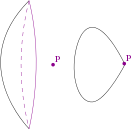
\includegraphics[width=5cm,height=3cm]{imagem/cw_esfera.pdf}
			\caption{Estrutura de CW-complexo de $S^{2 }$}
		\end{figure}
	\end{exemplo}

	
	\begin{exemplo}
		(Disco com alça) Sejam $p=(1,0), q=(-1,0) \in D^{2}$ e $I=[a,b] \subset \reta$. Temos $\partial I=\{a,b\}$. Definindo $f_{\partial_{0}}: \partial I \to D^{2}$ tal que $f_{\partial_{0}}(a)=p$ e $f_{\partial_{0}}(b)=q$ teremos o disco com alça $X=D^{2}\cup_{f_{\partial_{0}}}I$.
		
		\begin{figure}[!h]
			\centering
			\includegraphics[width=5cm,height=3cm]{imagem/disco_alca.pdf}
			\caption{Estrutura de CW-complexo do disco com alça.}
		\end{figure}   
	\end{exemplo}
	
	\begin{exemplo}
		(2-toro) Vamos exibir uma estrutura de CW-complexo para $T^{2}$. Representando o toro como o quadrado cujos os lados opostos estão identificados preservando a orientação, todos os vértices do quadrado serão identificados a um único ponto $p \in T^{2}$. Definamos o $0-$esqueleto como sendo $\skeleton{0} = \{p\}$. As arestas horizontais representam o mesmo $S^{1}$ no toro. Isso equivale a colar uma 1-célula ao 0-esqueleto, ou seja, $\skeleton{0}\cup_{f_{1\partial}}\celula{1}{1}$. Analogamente, as faces verticais também representam o mesmo $S^{1}$ no toro, o que indica que devemos anexar uma outra 1-célula o espaço anexado anteriormente, isto é, $\skeleton{0}\cup_{f_{1\partial}}\celula{1}{1}\cup_{f_{2\partial}}\celula{1}{2}$. Por fim, temos que anexar um 2-célula para cobrir o interior do quadrado. Então $T^{2} =\skeleton{2} = \skeleton{0}\cup_{f_{1\partial}}\celula{1}{1}\cup_{f_{2\partial}}\celula{1}{2}\cup_{f_{3\partial}}\celula{2}{3}$.
	\end{exemplo}
	
	\begin{exemplo}
		(n-espaço projetivo) Vamos exibir uma estrutura de CW-complexo para $\realprojetivo{n}$. Para $n=0$ temos que $\realprojetivo{0} = \{\classe{p}\}$, para um determinado $p \in \real{}$. Já para $n=1$, sabemos que existe um homeomorfismo $\realprojetivo{1} \approx S^{1}_{\sim} = \{\classe{p}: p \in S^{1},\; p \sim -p\}$. Note esse espaço quociente já possui, naturalmente, uma CW-estrutura pois, na passagem ao quociente, identificamos todos os pontos do equador com um único ponto desse conjunto. Digamos este ponto $p_{0} = (1,0)$, sem perda de generalidade. Isso quer dizer que ao colarmos uma 1-célula no ponto $p_{0}$ teremos $S^{1}_{\sim} \approx \{[p_{0}]\} \cup_{f}D^{1} \approx \realprojetivo{0}\cup_{f}D^{1} $ pois $\realprojetivo{0} \approx \{[p_{0}]\}$, portanto $ \realprojetivo{1} \approx \realprojetivo{0}\cup_{f}D^{1}$. Repetindo o procedimento anterior para $\realprojetivo{n} \approx S^{n}_{\sim} $ onde $p_{0} = (1,0,\dots, 0)$, teremos $\realprojetivo{n} \approx \realprojetivo{n-1} \cup_{f_{\partial}}D^{n}$. Assim, temos a CW-estrutura $\realprojetivo{j-1} \subseteq \realprojetivo{j}$ e $\realprojetivo{j} = \skeleton{j} \approx \skeleton{j-1}\cup_{f_{j\partial}}D^{j}$ para $1\leq j \leq n$.
	\end{exemplo}
	
	\begin{lema}\label{homologiacelular}
		(Homologia celular relativa) Sejam $A$ um anel comutativo com unidade e $X$ um CW-complexo, então
		$$
		\homologiarelskelesimpl{k}{n} \cong 
		\left\{
		\begin{array}{cc}
		\mathcal{C}_{n}(X), & k = n\\
		0, & k\neq n\\
		\end{array}
		\right.,
		$$
		onde $\mathcal{C}_{n}(X)$ é um $A-$módulo livre e finitamente gerado pelas $n-$células de $X$. Além disso,
		$$
		\mathcal{C}_{n}(X) \cong \somadir{\sigma} \homologiarelcel{n}{n}{\sigma} \cong \somadir{\sigma} A
		$$
		em que 
		$$
		\somadir{\sigma}f_{\sigma*}: \somadir{\sigma} \homologiarelcel{n}{n}{\sigma} \to \homologiarelskelesimpl{n}{n}
		$$
		denota o isomorfismo descrito.
	\end{lema}
	\begin{prova}
		Por definição, temos  $\skeleton{n} = \skeleton{n-1} \bigcup_{f_{\partial \sigma} } \celula{n}{\sigma}$ e também $\celula{n}{\sigma} \subset \skeleton{n}$, onde $f_{\sigma}:\celula{n}{\sigma} \to \skeleton{n}$ é a aplicação característica. Sejam $C_{\sigma}$ e $A_{\sigma}$ discos fechado e abertos, respectivamente, contendo o hemisfério norte de $f_{\sigma}(\celula{n}{\sigma})$. Definindo $N_{\sigma} = f_{\sigma}(\celula{n}{\sigma}) - C_{\sigma}$, $M_{\sigma} = f_{\sigma}(\celula{n}{\sigma}) - A_{\sigma}$ temos $\overline{N_{\sigma}} \subset M_{\sigma}$, e considerando $U = \skeleton{n} - \bigcup C_{\sigma}$, $Y = \skeleton{n} - \bigcup A_{\sigma}$ temos $U \subseteq Y$. Note que $\skeleton{n-1}$ é um retrato de deformação de $Y$, logo, pela invariância homotópica temos $\homologiarel{k}{\skeleton{n}}{\skeleton{n-1}} \cong  \homologiarel{k}{\skeleton{n}}{Y}$. Como $\skeleton{n} - U = \bigcup C_{\sigma}$ e $Y - U $ é homotópico a $\bigcup S^{n}_{\sigma}$, pelo teorema da excisão $\homologiarel{k}{\skeleton{n} - U}{Y- U} \cong \homologiarel{k}{\skeleton{n}}{Y}$. Portanto $\homologiarel{k}{\skeleton{n} - U}{Y- U} = \homologiarel{k}{\bigcup C_{\sigma}}{\bigcup S^{n}_{\sigma}} \cong \homologia{k}{\bigcup (\celula{n}{\sigma}, \celulabordo{n}{\sigma})} \cong \somadir{\sigma} \homologiarelcel{k}{n}{\sigma}$, pois $C_{\sigma} \approx \celula{n}{\sigma}$ e $S^{n}_{\sigma} = \celulabordo{n}{\sigma}$. Enfim, temos o diagrama comutativo:
		\[
		\xymatrix{
			\somadir{\sigma} \homologiarelcel{k}{n}{\sigma} \ar[r]^{id_{*}} \ar[d]^{\cong} & 
			\somadir{\sigma} \homologiarelcel{k}{n}{\sigma} \ar[r]^{id_{*}} \ar[d]^{\somadir{\sigma}f_{\sigma*}} & 
			\somadir{\sigma} \homologiarelcel{k}{n}{\sigma} \ar[d]^{\somadir{\sigma}f_{\sigma*}} 
			\\
			\homologiarel{k}{\skeleton{n} - U}{Y- U} \ar[r]^{\cong} & \homologiarel{k}{\skeleton{n}}{Y} \ar[r]^{\cong} & 
			\homologiarelskelesimpl{k}{n}.
		}
		\]
		Por fim, sabemos que $\homologiarelcel{k}{n}{\sigma} \cong A$ para $k=n$ e é trivial para $k\neq n$, então pela sequência anterior temos $\homologiarelskelesimpl{k}{n} \cong \somadir{\sigma}\homologiarelcel{k}{n}{\sigma} \cong \somadir{\sigma} A$ se $k=n$ e é trivial caso $k\neq n$, como desejávamos.
	\end{prova} 
	
	\begin{definicao}
		(Aplicação de Pares) Seja $X = \skeleton{n}$ um CW-complexo e tome $p \in \skeleton{n-1}$ como um ponto-base. Identificaremos um dado $q \in \skeleton{n}$ com o ponto-base se $q \in \skeleton{n-1}$, e diremos que $q \sim p$. Definimos $\skeleton{n}/\skeleton{n-1} = \{[q]: q \in \skeleton{n}, \; q \nsim p\}$ e a aplicação quociente $\pi : \skeleton{n} \to \skeleton{n}/\skeleton{n-1}$ por:
		$$
		\pi(q) = 
		\left\{
		\begin{array}{cc}
		\classe{p}, & q \in \skeleton{n-1}\\
		\classe{q}, & q \notin \skeleton{n-1}\\
		\end{array}
		\right..
		$$
		Seja $\bigvee_{\sigma} S^{n}_{\sigma}$ o buquet de $n-$esferas com o ponto-base $p$, então $\skeleton{n}/\skeleton{n-1} \approx \bigvee_{\sigma} S^{n}_{\sigma}$. Agora, definindo $s_{\sigma} : \skeleton{n}/\skeleton{n-1} \to S^{n}_{\sigma}$ por 
		$$
		\funcaocond{s_{\sigma}([q])}{q}{q \in \celula{n}{\sigma}}{p}{q \notin \celula{n}{\sigma}}
		$$
		chamamos de $\sigma-$aplicação de pares $p_{\sigma} = s_{\sigma} \circ \pi : (\skeleton{n}, \skeleton{n-1}) \to (S^{n}_{\sigma}, \{p\})$.
	\end{definicao}
	
	Denotaremos por $\Psi_{n}:\mathcal{C}_{k}(X) \to \homologiarelskelesimpl{k}{n}$ o isomorfismo definido no lema anterior dado por 
	$$
	\Psi(\sum_{\sigma} n_{\sigma} \sigma) = \sum_{\sigma} n_{\sigma} f_{\sigma *}[D^{n}],
	$$
	onde $[D^{n}]$ é um gerador do módulo $\homologiarelcel{n}{n}{}$.
	
	\begin{lema}
		(Inversa de $\Psi_{n}$) A aplicação inversa $\Phi_{n} : \homologiarelskelesimpl{n}{n} \to \mathcal{C}_{n}(X)$ do isomorfismo definido anteriormente é dada por
		$$
		\Phi_{n}(\alpha) = \sum_{\sigma} \phi_{n}(p_{\sigma *}\alpha)\sigma,
		$$
		onde $\phi_{n}: \homologiarel{n}{S^{n}}{\{p\}} \to \Lambda$ é o único homomorfismo tal que $\phi_{n}([S^{n}])=1$ e $[S^{n}]$ é a classe fundamental do par $(S^{n}, \{p\})$.
	\end{lema}
	\begin{prova}
		Mostremos a unicidade do homomorfismo. Sabemos que o grupo $\homologiarel{n}{S^{n}}{\{p\}}$ tem como geradores as classes $\{[S^{n}], [0]\}$ e como $\phi_{n}$ é homomorfismo, então $\phi_{n}([0]) = 0$. Definindo $\phi_{n}([S^{n}]) = 1$ e supondo que exista outro homomorfismo tal que $\phi_{n}^{'} ([S^{n}]) = 1$, então ambos homomorfismos coincidem quando avaliados nos geradores, logo $\phi_{n}^{'}=\phi_{n}$ o que é uma contradição, portanto $\phi_{n}$ é único. Sabemos o que $\Psi_{n}$ é um isomorfismo, então existe uma única aplicação $\Phi_{n}$ tal que $\Phi_{n} \circ \Psi_{n} = 1$. Tomando $\sigma$ uma $n-$célula geradora de $\mathcal{C}_{n}(X)$,
		$$
		\begin{aligned}
		\Phi_{n}(\Psi_{n}(\sigma)) 
		&= \sum_{\beta}\phi_{n}(p_{\beta *}\Psi_{n}(\sigma))\beta
		\\
		&= \sum_{\beta}\phi_{n}(p_{\beta *}f_{\partial\sigma *}[D^{n}])\beta
		\\
		&= \sum_{\beta}\phi_{n}((p_{\beta}\circ f_{\partial\sigma})_{*}[D^{n}])\beta
		\\
		&= \phi_{n}((p_{\sigma}\circ f_{\partial\sigma})_{*}[D^{n}])\sigma
		\\
		&= \phi_{n}([S^{n}])\sigma
		\\
		&= \sigma	
		\end{aligned},
		$$
		e como $\sigma \in \mathcal{C}_{n}(X)$ é arbitrário, então $\Phi_{n} \circ \Psi_{n} = 1$, como desejávamos.
	\end{prova}
	
	\begin{definicao}
		(Grau homológico) Seja $f: S^{n} \to S^{n}$ uma aplicação contínua e $f_{*}: \homologia{n}{S^{n}} \to \homologia{n}{S^{n}}$ o homomorfismo induzindo. Seja $[S^{n}] \in \homologia{n}{S^{n}}$ o gerador não-trivial desse grupo, então $f_{*}[S^{n}] = k[S^{n}]$ para algum $k \in \Lambda$. Denominamos $k=\deg(f)$ o grau homológico da aplicação $f$.
	\end{definicao}
	
	\begin{definicao}
		(Aplicação CW-bordo) Tome a tripla $(\skeleton{n}, \skeleton{n-1}, \skeleton{n-2})$ e a composição abaixo
		\[
		\xymatrix{
			\mathcal{C}_{n}(X) \ar[r]^{\Psi_{n}\qquad} &
			\homologiarelskelesimpl{n}{n} \ar[r]^{\delta_{*}} & 
			\homologiarelskele{n-1}{n-1}{n-2} \ar[r]^{\qquad \Phi_{n-1}}&
			\mathcal{C}_{n-1}(X)
		}
		\]
		onde $\delta_{*}$ é o homomorfismo de conexão da sequência da tripla. Denominamos por operador CW-bordo o homomorfismo $\partial_{n} = \Phi_{n-1} \circ \delta_{*} \circ \Psi_{n} : \mathcal{C}_{n}(X) \to \mathcal{C}_{n-1}(X)$.
	\end{definicao}
	
	\begin{teorema}
		(CW-bordo) A aplicação CW-bordo é um homomorfismo tal que $\partial_{n-1}\circ\partial_{n} = 0$ e é dado por:
		$$
		\partial_{n}(\sigma) = \sum_{\beta}[\beta:\sigma]\beta,
		$$
		onde $[\beta:\sigma]$ é o grau homológico da aplicação $p_{\beta} \circ f_{\partial\sigma}:\celulabordo{n}{\sigma} \to S^{n-1}_{\sigma}$.
	\end{teorema}
	\begin{prova}
		Por definição temos que $\partial_{n} = \Phi_{n-1} \circ \delta_{*} \circ \Psi_{n}$, logo é um homomorfismo.
		
		Consideremos o diagrama comutativo tal que na vertical temos a sequência exata longa do par $(\skeleton{n-1}, \skeleton{n-2})$
		$$
		\xymatrix{
			& \homologiaabrev{n-2}{\skeleton{n-2}}\ar[rd]^{j_{*}}
			\\
			\homologiarelskele{n}{n}{n-1} \ar[r]^{\delta_{*} \qquad}\ar[rd]_{\delta_{n}} &
			\homologiarelskele{n-1}{n-1}{n-2} \ar[u]^{\delta_{n-1}} \ar[r]^{ \delta_{*}}&
			\homologiarelskele{n-2}{n-2}{n-3}
			\\
			& \homologiaabrev{n-1}{\skeleton{n-1}}\ar[u]^{j_{*}}
		}
		$$
		Note que $\delta_{*} \circ \delta_{*} = j_{*} \circ \delta_{n-1} \circ j_{*} \circ \delta_{n}$. Pela exatidão da sequência vertical temos $Im(j_{*}) = Ker(\delta_{n-1})$, logo $\delta_{*}^{2}=0$. Com isso, temos o composição do CW-bordo $\partial_{n-1}\circ \partial_{n} = \Phi_{n-2} \circ \delta_{*} \circ \Psi_{n-1} \circ \Phi_{n-1} \circ \delta_{*} \circ \Psi_{n} = \Phi_{n-2} \circ \delta_{*}^{2} \circ \Psi_{n} =0$, pois $\Psi_{n-1} \circ \Phi_{n-1}=1$.
		
		Por definição temos $f_{\partial\sigma}: \celulabordo{n}{\sigma} \to \skeleton{n-1}$, assim temos o homomorfismo induzido $f_{\partial\sigma*}: \homologia{n-1}{\celulabordo{n}{\sigma} }\to \homologia{n-1}{\skeleton{n-1}}$. Analogamente, temos o homomorfismo $f_{\sigma*}:\homologiarelcel{n}{n}{\sigma} \to \homologiarelskelesimpl{n}{n}$ e o homomorfismo conectante $\delta_{n} : \homologiarelcel{n}{n}{\sigma} \to \homologia{n-1}{\celulabordo{n}{\sigma}}$ de modo que, tomanto $[\celula{n}{\sigma}] \in \homologiarelcel{n}{n}{\sigma}$ como um elemento gerador, então $\delta_{n}\circ f_{\sigma*}[\celula{n}{\sigma}] \in \homologia{n-1}{\skeleton{n-1}}$ é um elemento gerador. Por outro lado $f_{\partial\sigma*}\circ \delta_{n}[\celula{n}{\sigma}] \in \homologia{n-1}{\skeleton{n-1}}$ também é um elemento gerador, logo $f_{\partial\sigma*}\circ \delta_{n}[\celula{n}{\sigma}] = \lambda \delta_{n}\circ f_{\sigma*}[\celula{n}{\sigma}]$, para algum $\lambda \in \Lambda$. Como sempre podemos escolher um mapa caracteristico $f_{\sigma *}$ tal que $\lambda = 1$, temos $f_{\partial\sigma*}\circ \delta_{n} = \delta_{n}\circ f_{\partial\sigma*}$, e como $\delta_{*} = j_{*}\circ\delta_{n}$ então $f_{\partial\sigma*}\circ \delta_{*} = \delta_{*}\circ f_{\partial\sigma*}$. Assim, temos o operador CW-bordo
		$$
		\begin{aligned}
		\partial_{n}(\sigma) &= \Phi_{n-1}\circ\delta_{*}\circ\Psi_{n}(\sigma)
		\\
		&= \Phi_{n-1}\circ\delta_{*}\circ f_{\sigma*}([\celula{n}{\sigma}])
		\\
		&= \Phi_{n-1}\circ f_{\partial\sigma*}\circ\delta_{*}([\celula{n}{\sigma}])
		\\
		&= \Phi_{n-1}\circ f_{\partial\sigma*}\circ (j_{*}\circ \delta_{n}) ([\celula{n}{\sigma}])
		\\
		&= \Phi_{n-1} \circ f_{\partial\sigma*}([\celulabordo{n}{\sigma}])
		\\
		&= \sum_{\beta} \phi_{n-1}(p_{\beta*}\circ f_{\partial\sigma*}[\celulabordo{n}{\sigma}])\beta
		\\
		&= \sum_{\beta} \phi_{n-1}((p_{\beta}\circ f_{\partial\sigma})_{*}[S^{n-1}])\beta
		\\
		&= \sum_{\beta} \phi_{n-1}(\deg(p_{\beta}\circ f_{\partial\sigma})[S^{n-1}])\beta
		\\
		&= \sum_{\beta} \deg(p_{\beta}\circ f_{\partial\sigma})\phi_{n-1}([S^{n-1}])\beta
		\\
		&= \sum_{\beta} \deg(p_{\beta}\circ f_{\partial\sigma})\beta,
		\end{aligned}
		$$
		como desejávamos.
	\end{prova}
	
	\begin{teorema}\label{teorema_cw_homologia}
		(CW-homologia) Seja $X$ um CW-complexo, então existe uma identificação natural entre a CW-homologia $\mathcal{C}_{*}(X)$ e a homologia singular $\homologia{*}{X}$, isto é 
		$$
		\homologia{k}{X} \cong \homologia{k}{\mathcal{C}_{*}(X)}\; \forall k \in \inteiros.
		$$
	\end{teorema}
	\begin{proof}
		Para a demonstração desse resultado vamos considerar a sequência 
		$$
		\xymatrix{
			\mathcal{C}_{k+1}(X) \ar[r]^{\partial_{k+1}} & \mathcal{C}_{k}(X) \ar[r]^{\partial_{k}} & \mathcal{C}_{k-1}(X).
		}
		$$
		Por definição temos $\homologia{k}{\mathcal{C}_{*}(X)} = Ker(\partial_{k})/Im(\partial_{k+1})$, e com isso provaremos que 
		$$
		Ker(\partial_{k})/Im(\partial_{k+1}) \cong \homologia{k}{X}
		$$ 
		e então concluir a equivalência entre a CW-homologia e a homologia singular do espaço topológico $X$.
		
		Tomemos a sequência longa exata vertical da tripla $(\skeleton{k+1}, \skeleton{k-1}, \skeleton{k-2})$ e a sequência longa exata horizontal da tripla $(\skeleton{k+1}, \skeleton{k}, \skeleton{k-1})$  no diagrama abaixo:
		$$
		\xymatrix{
			& & \homologiarelskele{k}{k-1}{k-2}= 0 \ar[d]^{i_{*}} &
			\\
			& & \homologiarelskele{k}{k+1}{k-2} \ar[d]^{j_{*}} &
			\\
			\homologiarelskele{k+1}{k+1}{k} \ar[r]^{\quad\delta_{1*}} &		\homologiarelskele{k}{k}{k-1} \ar[r]^{i_{*}} \ar[rd]^{\delta_{2*}} & \homologiarelskele{k}{k+1}{k-1} \ar[r]^{j_{*}} \ar[d]^{\delta_{3*}} & \homologiarelskele{k}{k+1}{k}=0
			\\
			& & \homologiarelskele{k-1}{k-1}{k-2} &
		}
		$$
		onde $i_{*}, \; j_{*}$ e $\delta_{*}$ são as inclusões induzidas e o homomorfismo conectante, respectivamente. Seja $\classe{\alpha} \in \homologiarelskelesimpl{k}{k}$, então $\delta_{3*}\circ i_{*}\classe{\alpha} = \delta_{2*}\classe{\alpha}$.
		
		Vamos agora caracterizar $Ker(\delta_{2*})$. Dado $[\alpha] \in Ker(\delta_{2*})$, então $\delta_{3*}\circ i_{*}\classe{\alpha} = \delta_{2*}\classe{\alpha} = 0$. Como $i_{*}$ é um epimorfismo e $j_{*}$ é monomorfismo, então existe um único $\classe{\beta} \in \homologiarelskele{k}{k+1}{k-2}$ tal que $i_{*} \classe{\alpha} = j_{*} \classe{\beta}$. 
		
		Afirmo que $\phi: Ker(\delta_{2*}) \to \homologiarelskele{k}{k+1}{k-2}$ dado por $\phi(\classe{\alpha}) = \classe{\beta}$ é um epimorfismo. Seja $\classe{\beta'} \in \homologiarelskele{k}{k+1}{k-2}$, então existe um $\classe{\alpha'} \in \homologiarelskele{k}{k}{k-1}$ tal que $i_{*} \classe{\alpha'} = j_{*} \classe{\beta'}$. Com isso $\delta_{2*}\classe{\alpha'} = \delta_{3*}\circ i_{*}\classe{\alpha'} = \delta_{3*}\circ j_{*}\classe{\beta'} = 0$ pois $Im(j_{*}) = Ker(\delta_{3*})$, logo $\classe{\alpha'} \in Ker(\delta_{2*})$ e $\phi$ é epimorfismo.
		
		Como $\phi$ é sobrejetor, existe $\classe{\alpha} \in Ker(\delta_{2*})$ tal que $\phi(\classe{\alpha}) = 0$. Pela comutatividade do diagrama temos $i_{*}{\classe{\alpha}} = j_{*}\classe{0} = 0$, pois $j_{*}$ é monomorfismo, portanto $\classe{\alpha} \in Ker(i_{*})$ e, pela exatidão, temos $Ker(i_{*})=Im(\delta_{1*})$, logo $\classe{\alpha} \in Im(\delta_{1*})$. Com isso podemos concluir que $Ker(\phi) = Im(\delta_{1*})$. Pelo teorema fundamental do isomorfismo de grupos temos que $Ker(\delta_{2*})/Ker(\phi) \cong \homologiarelskele{k}{k+1}{k-2}$, ou seja, $Ker(\delta_{2*})/Im(\delta_{1*}) \cong \homologiarelskele{k}{k+1}{k-2}$.
		
		Sem perda de generalidade, vamos assumir que $X$ seja um CW-complexo de ordem $n$, isto é, $X= \skeleton{n}$. Fixemos um $0 \leq j \leq n$ e tomemos o $j-$ésimo esqueleto $\skeleton{j}$ e definamos $\skeleton{-1}$. Com isso, podemos escrever a sequência de homomorfismos de inclusão de pares:
		$$
		\xymatrix{
			\homologia{k}{\skeleton{j}} = \homologiarel{k}{\skeleton{j}}{\skeleton{-1}}\ar[r]& \homologiarel{k}{\skeleton{j}}{\skeleton{0}} \ar[r] & \dots \ar[r] & \homologiarel{k}{\skeleton{j}}{\skeleton{k-2}}
		}
		$$
		onde $k-2 \leq j$ e para cada $i-$ésimo termo $\homologiarelskele{k}{j}{i}$ no centro do diagrama abaixo, teremos a sequência exata de triplas nas verticais $(\skeleton{j}, \skeleton{i}, \skeleton{i-1})$, com $0\leq i +1\leq j$ com $h_{i}$ sendo os homomorfismos de inclusão:
		$$
		\xymatrix{
			\homologiarel{k}{\skeleton{i-1}}{\skeleton{i-2}}=0 \ar[d] & \homologiarel{k}{\skeleton{i}}{\skeleton{i-1}}=0 \ar[d] & \homologiarel{k}{\skeleton{i+1}}{\skeleton{i}}=0 \ar[d] &	
			\\
			\homologiarel{k}{\skeleton{n}}{\skeleton{i-2}} \ar[d]^{h_{i-1}} & \homologiarel{k}{\skeleton{n}}{\skeleton{i-1}} \ar[d]^{h_{i}} & \homologiarel{k}{\skeleton{n}}{\skeleton{i}} \ar[d]^{h_{i+1}}
			\\
			\homologiarel{k}{\skeleton{n}}{\skeleton{i-1}} \ar[r]\ar[d]^{\delta_{(i-1)*}}& \homologiarel{k}{\skeleton{n}}{\skeleton{i}} \ar[r] \ar[d]^{\delta_{i*}} &  \homologiarel{k}{\skeleton{n}}{\skeleton{i+1}} \ar[d]^{\delta_{(i+1)*}} 
			\\
			\homologiarelskele{k-1}{i-1}{i-2}=0& \homologiarel{k-1}{\skeleton{i}}{\skeleton{i-1}}=0 &  \homologiarel{k}{\skeleton{i+1}}{\skeleton{i}}=0. &		
		}
		$$
		Do Lema \ref{homologiacelular} temos que $\homologiarelskele{k}{i}{i-1} =0$ caso $k \neq i$, logo os grupos nas extemidades verticais do diagrama serão os triviais. Pela exatidão das sequências verticais temos $Im(h_{i}) = Ker(\delta_{i*})$, mas como $Im(\delta_{i*}) = 0 \Rightarrow Ker(\delta_{i*}) = \homologiarel{k}{\skeleton{n}}{\skeleton{i}}$, logo $h_{i}$ é um epimorfismo, portanto um isomorfismo, isto é, $\homologiarel{k}{\skeleton{n}}{\skeleton{i-1}} \cong \homologiarel{k}{\skeleton{n}}{\skeleton{i}}$, o que nos pertmite escrever a cadeia de isomorfismos 
		$$
		\begin{aligned}
		\homologia{k}{\skeleton{j}} &= \homologiarel{k}{\skeleton{j}}{\skeleton{-1}} 
		\\
		&\cong  \homologiarel{k}{\skeleton{j}}{\skeleton{0}} \cong \dots \cong  \homologiarel{k}{\skeleton{j}}{\skeleton{i}} \cong  \dots \cong \homologiarel{k}{\skeleton{j}}{\skeleton{k-2}},
		\end{aligned}
		$$
		logo $\homologia{k}{\skeleton{j}} \cong \homologiarel{k}{\skeleton{j}}{\skeleton{i}}$.
		
		Por fim, como supusemos que $X = \skeleton{n}$ e a construção anterior vale para $j = n$, então $\homologia{k}{X} = \homologia{k}{\skeleton{n}} \cong \homologiarelskele{k}{n}{i}$.
		
		Assim, $\homologia{k}{X} \cong \homologiarel{k}{\skeleton{k+1}}{\skeleton{k-2}} \cong Ker(\delta_{2*})/Im(\delta_{1*})$. Mas como $\partial_{k} = \Phi_{n-1}\circ\delta_{*}\circ\Psi_{n}$, então $Ker(\delta_{2*}) \cong Ker(\partial_{k})$ e $Im(\delta_{1*}) \cong Im(\partial_{k+1})$, logo $Ker(\delta_{2*})/Im(\delta_{1*}) \cong Ker(\partial_{k})/Im(\partial_{k+1}) = \homologia{k}{\mathcal{C}_{*}}$, logo $\homologia{k}{X} \cong \homologia{k}{\mathcal{C}_{*}}$ que é a equivalência entre as homologias, como desejávamos.
	\end{proof}
	
	\begin{exemplo}
		(CW-homologia da n-esfera)
		Vamos exibir uma estrutura de CW-complexo para $S^{n}$. Para isso tomemos um ponto $p \in S^{n}$ e definamos o $0-$skeleton $\skeleton{0}=\{p\}$. Em seguida, anexemos uma $n-$célula a $\skeleton{0}$ onde $f_{\partial}: \celulabordo{n}{} \to \skeleton{0}$, isto é, $\skeleton{n} = \{p\}\cup_{f_{\partial}} \celula{n}{}$ (veja a Figura \ref{figura_cw_n_esfera}). Pelo teorema da CW-homologia temos que $\homologia{k}{S^{n}} \cong \homologiarelskelesimpl{k}{k}$, logo $\homologia{0}{S^{n}} \cong \homologiarelskelesimpl{0}{0} \cong \Lambda$, $\homologia{n}{S^{n}} \cong \homologiarelskelesimpl{n}{n} \cong \Lambda$ e $\homologia{k}{S^{n}} \cong \homologiarelskelesimpl{k}{j} =0$ caso $k \neq j$, logo
		$$
		\homologia{*}{S^{n}} = \homologia{0}{S^{n}}\oplus\homologia{n}{S^{n}} \cong \Lambda\oplus\Lambda.
		$$
		\begin{figure}[!h]
			\centering
			\includegraphics[width=9cm,height=5cm]{imagem/cw_n_esfera.pdf}
			\caption{Estrutura de CW-complexo da n-esfera $S^{n}$.}
			\label{figura_cw_n_esfera}
		\end{figure} 
	\end{exemplo}
	
	\begin{figure}[!h]
		\centering
		\includegraphics[width=13cm,height=7cm]{imagem/cw_2_toro.pdf}
		\caption{Estrutura de CW-complexo do 2-toro $T^{2}$.}
		\label{figura_cw_2_toro}
	\end{figure} 
	
	\begin{exemplo}
		(CW-homologia do 2-toro) Vamos exibir uma estrutura de CW-complexo para $T^{2}$. Para isso tomemos a identificação do toro com o quadrado cujo os lados opostos serão identificados, assim os vertices do quadrado serão um ponto $p \in T^{2}$ e definindo o $0-$skeleton $\skeleton{0} = \{p\}$, agora vamos anexar às faces do quadrado duas $1-$células, isto é, $\skeleton{1} = \skeleton{0}\cup_{f_{1\partial}}\celula{1}{1}\cup_{f_{2\partial}}\celula{1}{2}$, e por fim, cobrir o centro do quandrado anexando um $2-$célula, com isso, $\skeleton{2} = \skeleton{1}\cup_{f_{3\partial}}\celula{2}{3}$ (veja a Figura \ref{figura_cw_2_toro}). Então
		$$
		T^{2} =\skeleton{2} = \skeleton{0}\cup_{f_{1\partial}}\celula{1}{1}\cup_{f_{2\partial}}\celula{1}{2}\cup_{f_{3\partial}}\celula{2}{3}.
		$$
		
		Teremos os grupos de homologia não-triviais:
		$$
		\begin{aligned}
		\homologia{0}{T^{2}} &\cong \homologiarelskele{0}{0}{-1} \cong \Lambda,
		\\
		\homologia{1}{T^{2}} &\cong \homologiarelskele{1}{1}{0} \cong \somadir{i=1,2}\homologiarelcel{1}{1}{i} \cong \somadir{i=1,2}\Lambda
		\\
		\homologia{2}{T^{2}} &\cong \homologiarelskele{2}{2}{1} \cong \Lambda.
		\end{aligned}
		$$
		Logo,
		$$
		\\
		\homologia{*}{T^{2}} = \homologia{0}{T^{2}}\oplus\homologia{1}{T^{2}} \oplus\homologia{2}{T^{2}}\cong \Lambda\oplus\Lambda\oplus\Lambda\oplus\Lambda.
		$$
	\end{exemplo}	
	
	
	\chapter{Teoria de Morse}\label{capitulo_teoria_morse}
	Na investigação da topologia de variedades o principal objetivo é a determinação de seus invariantes topológicos, ou seja, características das variedades que são invariantes por homeomorfismos. Algumas abordagens são algébricas, tais como: a determinação de seus grupos de homotopia, seus grupos de homologia e cohomologia. Outras são diferenciais, tais como: teoremas de mergulho, transversalidade, teorema de Sard, etc. A Teoria de Morse faz uma conexão entre as duas metodologias. Através de uma função suave definida na variedade, determina-se seus pontos críticos, e através deles se constrói um $CW$-complexo cuja homologia coincide com a homologia singular da variedade, o que pode ser encontrado na Seção $\ref{secao_cw_complexo}$. O que torna a Teoria de Morse uma das construções matemáticas mais bonitas do século XX é justamente essa conexão entre as diferentes descrições.
	
	O propósito desse capítulo é de apresentação rápida do formalismo e alguns dos principais resultados para que possamos estender a construção aqui feita para a homologia de variedades de dimensão infinita (Homologia de Floer). Os detalhes das demonstrações e técnicas utilizadas podem ser encontrados em $\cite{milnor}$ e $\cite{banyaga_morse_homology}$.
	
	\begin{definicao}\label{definicao_variedade_fechada}
		(Variedade fechada) Seja $M$ uma n-variedade diferencial. Diz-se que $M$ é fechada se é compacta e sem bordo.
	\end{definicao}
	
	De agora em diante $M$ será uma $n$-variedade Riemanniana diferenciável fechada, cujas definições podem ser encontradas no Apêndice \ref{apendice_variedade_riemanniana}.
	
	\section{Teoria de Morse Clássica}\label{secao_morse_classica}
	
	\begin{definicao}
		(Função de Morse) Sejam $M$ uma n-variedade fechada, $f \in \funcoessuaves{M}$ e $\pontoscriticos{f} = \{p \in M: df_{p} = 0\}$ o conjunto dos pontos críticos de $f$. Dizemos que $f$ é uma função de Morse se a hessiana $H_{p}(f)$ é não-degenerada para todo $p \in \pontoscriticos{f}$. O conjunto das funções de Morse definidas em $M$ será denotado por $\funcoesmorse{M}$. 
	\end{definicao}

	O índice de Morse de um dado $p \in \pontoscriticos{f}$ é a dimensão do maior subespaço $V\subset T_{p}M $ tal que \ hessiana é negativa-definita, isto é, $H_{p}(f)(v,u)<0$ para todo $v,u \in V$. Denotaremos esse índice por $\lambda_{p} = dim(V)$. Como a hessiana é não-degenerada, então $H_{p}(f)$ é diagonalizável e o número de auto-valores negativos é o índice $\lambda_{p}$.
	
	\begin{lema}
		(Lema de Morse) Sejam $f \in \funcoesmorse{M}$ e $p \in \pontoscriticos{f}$ com índice de Morse $\lambda_{p}$. Então existe uma carta $\{U, \phi\}$ de $p$ com $\phi(p)=0 \in \real{n}$ tal que 
		$$
		\begin{aligned}
		(f\circ \phi^{-1})(x_{1}, \dots, x_{n}) &= f(p)-x_{1}^{2}-\dots -x^{2}_{\lambda_{p}}+x^{2}_{\lambda_{p}+1}+\dots + x^{2}_{n}
		\\
		&=f(p)+x^{t}Dx,
		\end{aligned}
		$$
		onde $D$ é a representação diagonal de $H_{p}(f)$.
	\end{lema}
	
	\begin{observacao}
		Como consequência do Lema de Morse, pode-se mostrar que os pontos críticos de uma função de Morse $f \in \funcoesmorse{M}$ são isolados. Pela compacidade de $M$ tem-se que os pontos isolados são finitos.
	\end{observacao}
	
	
	A existência das funções de Morse é ilustrada pelo seguinte exemplo. Seja $f:M\to \reta$ tal que $f(x_{1}, \dots, x_{n}) = x_{n}$. Essa função é chamada de função altura e pode-se mostrar que $f$ é uma função de Morse, logo $\funcoesmorse{M} \neq \emptyset$.
	
	\begin{exemplo}
		Sejam $S^{2} \subset \real{3}$ a 2-esfera centrada na origem e $f:S^{2}\to \reta$ a função altura dadar por $f(x,y,z) = z$. Os pontos críticos de $f$ são $p_{\pm} = \{(0,0,\pm 1)\}$, cujos índices são $\lambda_{p_{-} } = 0$ e $\lambda_{p_{+}} = 2$.
	\end{exemplo}
	
	As funções de Morse não são um caso raro nessa descrição, muito pelo contrário. O seguinte teorema garante que tais funções são abundantes no conjunto das funções suaves e tal resultado pode ser encontrado em $\cite{amyia_diff_topology}$.
	
	\begin{teorema}
		Seja $g\in \funcoessuaves{M}$. Então existe $f \in \funcoesmorse{M}$ suficientemente próxima a $g$, isto é, $\funcoesmorse{M}$ é denso em $\funcoessuaves{M}$.
	\end{teorema} 
	
	Dado $a \in \reta$, definimos o conjunto $M^{a}= f^{-1}((-\infty, a]) = \{p \in M: f(p)\leq a\}$ como sendo o conjunto em $M$ de nível $a$. Uma consequência imediata é que, dados $a\leq b \in \reta$, então $M^{a} \subseteq M^{b}$.
	
	\begin{teorema}
		Sejam $f \in \funcoesmorse{M}$ e $a<b \in \reta$ tais que $f^{-1}([a,b])\subset M$ não contenha pontos críticos de $f$. Então $M^{a}$ é difeomorfo a $M^{b}$. Além disso, $M^{a}$ é um retrato de deformação de $M^{b}$, de modo que a inclusão  $M^{a} \hookrightarrow M^{b}$ é uma equivalência homotópica.
	\end{teorema}
	
	O seguinte teorema afirma que, fixando $a \in \reta$ e variando $t \in \reta$, se $f^{-1}([a,t]) \cap \pontoscriticos{f} \neq \emptyset$, os conjuntos de nível $M^{a}$ e $M^{t}$ não podem ser deformados um no outro.
	
	\begin{teorema}\label{teorema cw_complexo_ponto_critico_morse}
		Sejam $f\in \funcoesmorse{M}$ e $p\in \pontoscriticos{f}$ com índice $\lambda_{p}$ tal que $f(p) = c$. Suponhamos que$f^{-1}([c-\epsilon,c+\epsilon])\cap \pontoscriticos{f} = \{p\}$ para algum $\epsilon>0$. Então o conjunto de nível $M^{c+\epsilon}$ tem o mesmo tipo de homotopia de $M^{c+\epsilon}$ com uma $\lambda_{p}$-célula colada, isto é, $M^{c+\epsilon} \simeq M^{c-\epsilon}\cup_{f_{\partial}} D^{\lambda_{p}}$.
	\end{teorema}
	
	\begin{observacao}
		O teorema anterior tem como hipótese a exitência de apenas um ponto crítico em $f^{-1}([c-\epsilon,c+\epsilon])$. No caso em que $f^{-1}([c-\epsilon,c+\epsilon]) \cap \pontoscriticos{f} = \{p_{j}\}_{j=1}^{r}$, teremos $M^{c+\epsilon} \simeq M^{c-\epsilon}\cup_{f_{\partial_{1}}} D^{\lambda_{1}}\dots  \cup_{f_{\partial_{r}}} D^{\lambda_{r}}$.
	\end{observacao}
	
	\begin{observacao}
		Uma consequência imediata do teorema anterior é que, supondo $p \in \pontoscriticos{f}$ e tomando $a = f(p)$, temos que $M^{a}$ é um $CW$-complexo. 
	\end{observacao}
	
	Supondo que $M$ seja compacto e conexo, então $f(M) = [a,b] \subset \reta$ é um compacto. Suponha que $\pontoscriticos{f} = \{p_{j}\}_{j=1}^{k}$, $\lambda_{j}$ seja o índice do j-ésimo ponto crítico e que exista uma partição $t_{1} = a < t_{2}< \dots< t_{k+1} = b$ tal que $f^{-1}((t_{k}, t_{k+1})) \cap \pontoscriticos{f} = \{p_{k}\}$. Ao variarmos $t \in [a,b]$ teremos a construção do $CW$-complexo
	$$
	\begin{aligned}
	M^{t_{1}} &\simeq \{p_{1}\}
	\\
	M^{t_{2}} & \simeq \{p_{1}\} \cup_{f_{\partial_{1}}} D^{\lambda_{1}}
	\\
	\vdots&
	\\
	M = M^{t_{k+1}} &\simeq\{p_{1}\} \cup_{f_{\partial_{1}}} D^{\lambda_{1}}\dots  \cup_{f_{\partial_{k}}} D^{\lambda_{k}}.
	\end{aligned}
	$$
	
	Caso existam pontos críticos distintos com valores críticos coincidentes a mesma construção pode ser feita perturbando a função de Morse $f$ de modo a obter uma outra $f' \in \funcoesmorse{M}$ com os mesmos pontos críticos agora com valores críticos todos distintos. Essa construção é viabilizada pela densidade das funções de Morse em $\funcoessuaves{M}$.
	
	\begin{exemplo}
		(2-toro) Sejam $T^{2} \subset \real{3}$ o toro centrado na origem do plano $Oy\times Ox = \{(x, y ,0) \in \real{3}\}$ e $\varphi:[0,2\pi]\times [0,2\pi] \to \real{3}$ uma parametrização dada por 
		$$
		\varphi(\theta, \phi) = ((2+\cos\phi)\cos\theta, (2+\cos\phi)\sin\theta, \sin\phi).
		$$
		
		Com isso, tem-se que o espaço tangente $T_{p}T^{2} $ é gerado por $ \{\derivadaparcialabrev{\theta}, \derivadaparcialabrev{\phi} \}|_{p}$ onde
		$$
		\begin{aligned}
			\derivadaparcialabrev{\theta} &= -(2+\cos\phi)\sin\theta \derivadaparcialabrev{x}+(2+\cos\phi)\cos\theta \derivadaparcialabrev{y},
			\\
			\derivadaparcialabrev{\phi} &=  - \sin\phi \cos\theta 	\derivadaparcialabrev{x} - \sin\phi \sin\theta 	\derivadaparcialabrev{y} +\cos\phi				\derivadaparcialabrev{z}.
			\end{aligned} 
		$$
				
		Seja $f:T^{2} \to \reta$ a função largura $f(x,y,z)=x$. Tem-se que o diferencial de $f$ e $df_{p} = \derivadaparcialabrev{x}$. Com isso, dado $v \in \real{3}$ tem-se que $df_{p}(v) = \produtointerno{\nabla f(p)}{v}  = \produtointerno{(1,0,0)}{(v_{x}, v_{y}, v_{z})} =v_{x}$. Assim, o caso em que $df_{p}(v) = 0$ implica que $v_{x} = 0$, ou seja, os vetores dos espaços tangentes não podem ter componentes na direção $Ox$. Com isso, basta que os elementos da base não o tenham, isto é, $\sin\phi = \sin\theta = 0$. Portanto, $\phi, \theta \in \{0, \pi\}$ e os pontos críticos de $f$ são $\varphi(0,0) = (3,0,0)$, $\varphi(0,\pi) = (-1,0,0)$, $\varphi(\pi,0) = (-3,0,0)$ e $\varphi(\pi,\pi) = (1,0,0)$, os quais estão ilustrados na Figura \ref{figura_toro_funcao_altura}.
			
		Assim, a representação matricial da Hessiana $H_{p}(f)$ é
			$$
			H(\phi, \theta) = 
			\left(
			\begin{array}{cc}
			-(2+\cos\phi)\cos\theta & \sin\phi \sin\theta  
			\\
			\sin\phi \sin\theta   & -\cos\phi \cos\theta  
			\end{array}
			\right).
			$$
		Avaliando a hessiana nos pontos críticos tem-se
			$$
			H(0, 0) = 
			\left(
			\begin{array}{cc}
			-3 & 0
			\\
			0& -1
			\end{array}
			\right),
			H(0, \pi) = 
			\left(
			\begin{array}{cc}
			3 & 0
			\\
			0& 1
			\end{array}
			\right)
			$$
			$$
			H(\pi, 0) = 
			\left(
			\begin{array}{cc}
			-1 & 0
			\\
			0& 1
			\end{array}
			\right),
			H(\pi, \pi) = 
			\left(
			\begin{array}{cc}
			1 & 0
			\\
			0& -1
			\end{array}
			\right)
			$$
			
			Com isso, os índices $\lambda_{(\phi, \theta)}$ dos pontos críticos são: $\lambda_{(0,0)} = 2$, $\lambda_{(0,\pi)} = 0$, $\lambda_{(\pi,0)} = 1$ e $\lambda_{(\pi,\pi)} = 1$.
			
			\begin{figure}[!h]
				\centering
				\includegraphics[width=8cm,height=7cm]{imagem/toro_funcao_altura.pdf}
				\caption{Pontos críticos da função altura em $T^{2}$.}
				\label{figura_toro_funcao_altura}
			\end{figure}
	\end{exemplo}

	Originalmente, a relação entre a topologia de $M$ e os pontos críticos de uma função de Morse $f:M \to \reta$, foi dada em termos de desigualdades, chamadas desigualdades de Morse.
	
	\begin{definicao}
		(Números de Betti) O j-ésimo número de Betti de $M$ é o inteiro $\beta_{j}(M) = dim(H_{j}(M))$, onde $H_{j}(M)$ é o j-ésimo grupo de homologia singular de $M$.
	\end{definicao}
	
	Como os grupos de homologia de $M$ são invariantes topológicos, então os números de Betti de $M$ também são.
	
	Seja $f \in \funcoesmorse{M}$. O número de pontos críticos de índice $k$ é denotado por $\nu_{k}$. Note que $\beta_{k}(M)$ contém as informações sobre a topologia da variedade, por outro lado, $\nu_{k}$ contém as informações sobre os pontos críticos de $f$.
	
	\begin{teorema}
		(Desigualdades de Morse) Sejam $f \in \funcoesmorse{M}$ e $\nu_{k}$ o número de pontos críticos de $f$ com índice de Morse $k$. Então valem as seguintes desigualdades:
		\begin{enumerate}
			\item $\beta_{k}(M) \leq \nu_{k}$ para $0\leq k\leq n$,
			
			\item $\sum_{j = 0}^{k}(-1)^{k-j}\beta_{j}(M) \leq \sum_{j = 0}^{k}(-1)^{k-j}\nu_{j} $ para $0 \leq k \leq n$ e vale a igualdade para o caso em que $k=n$.
		\end{enumerate}
	\end{teorema}
	
	\begin{observacao}
		No caso da igualdade do segundo item do teorema temos a característica de Euler-Poincaré $\chi(M) = \sum_{j = 0}^{n}(-1)^{n-j}\beta_{j}(M)$, que também é um invariante topológico e é a generalização do teorema de Euler para poliedros convexos $V-A+F = 2$, onde $V$ é o número de vértices, $A$ é o número de arestas e $F$ é o número de faces.
	\end{observacao}
	
	
	\section{Teoria de Morse-Witten}
	\subsection{Fluxos Gradiente e Variedades de Conexão}\label{secao_fluxo_gradiente}
	Sejam $X \in \campossuaves{M}$ um campo vetorial suave em $M$ e $p \in M$. Sabe-se que existe uma curva $\gamma: \reta\to M$ que é solução do sistema de equações diferenciais 
	$$
	\derivada{\gamma(t)}{t} = X(\gamma(t)), \; \gamma(0) = p.
	$$
	Como $M$ é compacta e sem bordo, então a solução $\gamma = \gamma_{p}$ existe para todo $t\in \reta$. A aplicação $\phi: \retacartesianovariedade\to M$ definida por $\phi(t,p) = \gamma_{p}(t)$ é chamada de fluxo gerado por $X$ e, fixado $p\in M$, a curva $\gamma_{p}:\reta\to M$ é chamada de linha do fluxo de $X$. Como o fluxo $\phi$ está bem-definido para todo $t \in \reta$, então podemos efetuar a composição $\phi_{s}\circ\phi_{t}(p) = \phi(s+t, p)$ para todo $p\in M$, logo $\phi_{s}\circ\phi_{t} = \phi_{s+t}$ e $\phi_{0} = Id$.
	\begin{definicao}
		(Órbitas) A órbita de $p \in M$ pelo fluxo $\phi$ é a imagem da curva $\phi^{p} = \phi(.,p):\reta\to M$ e será denotada por $\orbitaponto{p}$. As órbitas podem ser de três categorias
		\begin{enumerate}
			\item Singular, se $\orbitaponto{p}$ = \{p\}.
			
			\item Fechada, se existe $\tau \in \reta$ tal que $\phi_{\tau+t}(p) = p$ para todo $t \in \reta$.
			
			\item Regular, quando não é singular e não é fechada.
		\end{enumerate}
		
	\end{definicao}
	
	Pela compacidade de $M$ e pela unicidade da solução do problema de valor inicial anteriormente descrito, temos que $\orbitaponto{p}\subset M$ é uma imersão injetiva quando é uma órbita regular. Vista como um subconjunto de $\real{m}$, para um inteiro $m>0$ suficientemente grande (Teorema de Megulho de Whitney $\cite{guillemin_differential_topology}$), $M$ é um conjunto limitado, logo $\orbitaponto{p}$ também é limitado. Assim, tal órbita admite pontos limites. Os conjunto $\alpha$-limite e $\omega$-limite de $p \in M$ são definidos por $\alpha(p) = \{q \in M: \phi_{t}(p) \to q, t \to -\infty\}$ e $\omega(p) = \{q \in M: \phi_{t}(p) \to q, t \to \infty\}$. O seguinte resultado sobre a topologia dos conjuntos limites é feito em $\cite{palis_dynamical_systems}$.
	
	\begin{proposicao}
		Sejam $M$ uma variedade compacta e $X\in \campossuaves{M}$. Então para $p \in M$ tem-se, que $\alpha(p)$ e $\omega(p)$ são fechados, conexos e invariantes pelo fluxo de $X$, isto é, são uniões de órbitas de $X$.
	\end{proposicao}
	
	Vamos trabalhar com o campo gradiente da função de Morse $f$ pois dele podemos extrair informações sobre o comportamento dessa função. Munindo $M$ com uma métrica Riemanniana $g: T_{p}M \times T_{p}M \to \reta$, temos que $df_{p}(v) = g(\nabla f(p), v)$, onde $v \in T_{p}M$. Sejam $-\gradiente \in \campossuaves{M}$ e $\gamma$ a curva integral de $-\gradiente $ tal que $\gamma(0) = p\in M$. Então
	$$
	\begin{aligned}
	\derivada{}{t}(f \circ \gamma)(t) &= g(\gradiente(\gamma(t)), \dot{\gamma}(t)) 
	\\
	&=g(\gradiente(\gamma(t)), -\gradiente(\gamma(t))) 
	\\
	&= -\norma{\gradiente(\gamma(t))}^{2}
	\\
	&\leq 0,
	\end{aligned}
	$$
	para todo $t \in \reta$.
	
	Isso mostra que a função de Morse $f$ é decrescente ao longo das linhas de fluxo do campo gradiente negativo. Além disso, supondo que $\gamma(0) =p\in \pontoscriticos{f}$, então a desigualdade acima atinge seu maior valor em $t=0$, pois $df_{p }= 0$. Como $f$ é decrescente e atinge seu máximo em $t=0$, então a órbita $\orbitaponto{p}$ é regular e não-fechada. Em $\cite{palis_dynamical_systems}$ mostra-se que, para todo $q \in M$ tem-se que $\orbitaponto{q}$ intersecta $f^{-1}(f(q))$ transversalmente. Além disso, os pontos limites das órbitas são pontos críticos, ou seja, $\alpha(q)\cup\omega(q) \subset \pontoscriticos{f}$.
	
	Sabemos que, se $f \in \funcoesmorse{M}$, então $\pontoscriticos{f}$ é um conjunto finito. Com isso, pode-se mostrar, 
	
	\begin{lema}\label{lema_conjunto_limite_funcao_morse}
		Se 
		$p \in M$, então $\alpha(p)  = \{q\}$ e $\omega(p) = \{r\}$ onde $q, r \in \pontoscriticos{f}$.
	\end{lema}
	
	\begin{definicao}
		(Variedades instáveis/estáveis)  As variedades instável e estável de um ponto $p \in \pontoscriticos{f}$ são os conjutos $\variedadeinstavel{p} = \{q\in M: \phi_{t}(q) \to p,\; t\to -\infty\}$ e $\variedadeestavel{p} = \{q\in M: \phi_{t}(q) \to p,\; t\to \infty\}$.
	\end{definicao}
	
	\begin{observacao}
		Em termos de pontos limite, podemos reescrever as variedades instáveis e estáveis de $p \in \pontoscriticos{f}$ como sendo $\variedadeinstavel{p} = \{q\in M: \alpha(q)=p\}$ e $\variedadeestavel{p} = \{q\in M: \omega(q)=p\}$.
	\end{observacao}
	
	Da observação anterior, podemos afirmar que ambas as variedades instável e estável dos pontos críticos são contráteis. De fato, defina $Id: M\to M$ como sendo a aplicação identidade e $c:M\to M$ como sendo a aplicação constante $c(M) =\{p\} $, onde $p \in \pontoscriticos{f}$. Então $h:\intervalo\times \variedadeinstavel{p} \to \variedadeinstavel{p}$ tal que $h(t,q) = \phi(t/(1-t), q)$ é uma homotopia entre $Id$ e $c$, pois é contínua e $h(0, q) = Id(q)$ e $\lim_{t \to 1}h(t, q) = c(q)$, logo a variedade instável é contrátil. Com uma argumento análogo mostra-se que $\variedadeestavel{p}$ é contrátil.
	
	Definimos o espaço tangente instável como sendo o subespaço $\espacotangentevariedadeinstavel\subset \espacotangentevariedade$ tal que a restrição da Hessiana $\hessianaponto{p}{f}$ a $\espacotangentevariedadeinstavel$ é negativa-definida. Analogamente temos o espaço tangente estável $\espacotangentevariedadeestavel \subset \espacotangentevariedade$, onde a Hessiana é positiva-definida. Com isso, segue o teorema da variedade estável, cuja demonstração pode ser encontrada em $\cite{banyaga_morse_homology}$.
	
	\begin{teorema}\label{teorema_variedade_instavel_estavel}
		(Teorema da variedade instável/estável) Sejam $f \in \funcoesmorse{M}$ e $p \in \pontoscriticos{f}$. Então temos a decomposição $\espacotangentevariedade=\espacotangentevariedadeinstavel\oplus\espacotangentevariedadeestavel$. Além disso, existem mergulhos suaves e sobrejetores $\espacotangentevariedadeinstavel \hookrightarrow \variedadeinstavel{p} \subseteq M$ e $\espacotangentevariedadeestavel \hookrightarrow \variedadeestavel{p} \subseteq M$. Com isso, $\variedadeinstavel{p}$ e $\variedadeestavel{p}$ são subvariedades sem bordo com dimensão $\lambda_{p}$ e $n-\lambda_{p}$, respectivamente.
	\end{teorema}
	
	\begin{observacao}
		Do mergulho dado pelo teorema anterior temos, que as variedades instável e estável possuem o mesmo tipo de homotopia de um disco aberto cujas dimensões são $\lambda_{p}$ e $n-\lambda_{p}$, respectivamente.
	\end{observacao}

	Podemos decompor a variedade $M$ como a união disjunta das variedades instáveis ou união disjunta da variedades estáveis, o que é garantido pelo resultado a seguir.
	
	\begin{proposicao}\label{proposicao_uniao_variedade_instavel_estavel}
		Se $f \in \funcoesmorse{M}$, então
		$$
		M = \dot{\bigcup_{p \in \pontoscriticos{f}}}\variedadeestavel{p} = \dot{\bigcup_{p \in \pontoscriticos{f}}}\variedadeinstavel{p}.
		$$
	\end{proposicao}

	 O propósito das definições desse ponto em diante é a construção de um complexo de cadeia associado ao fluxo gradiente de uma função de Morse com uma propriedade adicional, que chamaremos de propriedade de transversalidade entre as variedades instáveis e estáveis.
	 
	 \begin{definicao}
	 	(Variedade Conectante e o Espaço Moduli) Sejam $f \in \funcoesmorse{M}$ e $p,q \in \pontoscriticos{f}$. A variedade conectante de $p$ e $q$ é definida por $\variedadeconectantepontos{p}{q} = \variedadeinstavel{p}\cap \variedadeestavel{q}$. Seja $c \in (f(q), f(p)) \subset \reta$ um valor regular de $f$. Então o espaço moduli de $p$ e $q$ é definido por $\espacomoduli{p}{q} = \variedadeconectantepontos{p}{q}\cap f^{-1}(c)$.
	 \end{definicao}
	 
	 \begin{definicao}\label{definicao_aplicao_transversal}
	 	(Aplicações tranversais) Sejam $f: N\to M$ e $g: Z \to M$ duas aplicações suaves entre variedades diferenciáveis. Dizemos que $f$ é transversal a $g$, e denotemos $f \pitchfork g$, sempre que $f(x) = g(z) = y$ tem-se $df_{x}(\espacotangenteponto{x}{N}) + dg_{z}(\espacotangenteponto{z}{Z}) = \espacotangenteponto{y}{M} $.
	 \end{definicao}
	 
	 \begin{observacao}
	 	Se $Z \subseteq M$ e $g$ é a aplicação de inclusão, então denotaremos a transversalidade por $f\pitchfork Z$. Trataremos constatemente os casos em que $N, Z \subseteq M$ e $f$ e $g$ são as inclusões e denotaremos a transversalidade por $N \pitchfork Z$.
	 \end{observacao}
	 
	 \begin{definicao}
	 	(Funções de Morse-Smale) Dizemos que o gradiente negativo de $f \in \funcoesmorse{M}$ satisfaz a condição de Morse-Smale se $\variedadeinstavel{p}\pitchfork \variedadeestavel{q}$ para todos $p,q \in \pontoscriticos{f}$. O conjuntos dessas funções é denotado por $\funcoesmorsesmale{M}$.
	 \end{definicao}
	 
	 \begin{teorema}
	 	Sejam $f\in \funcoesmorsesmale{M}$ e $p,q \in \pontoscriticos{f}$. Então a variedade conectante $\variedadeconectantepontos{p}{q}$ e o espaço moduli $\espacomoduli{p}{q}$ são vazios ou subvariedades de $M$ sem bordo cujas dimensões são $dim(\variedadeconectantepontos{p}{q}) = \lambda_{p} -\lambda_{q}$ e $dim(\espacomoduli{p}{q}) = \lambda_{p} -\lambda_{q}-1$. 
	 \end{teorema}
	 
	 \begin{proposicao}
	 	Sejam $f \in \funcoesmorsesmale{M}$ e $p,q \in \pontoscriticos{f}$.
	 	\begin{enumerate}
	 		\item Se $\lambda_{p}<\lambda_{q}$, então $\variedadeconectantepontos{p}{q} = \emptyset$,
	 		
	 		\item $\variedadeconectantepontos{p}{p} = \{p\}$
	 		
	 		\item Se $\lambda_{p} = \lambda_{q}$ e $p\neq q$, então $\variedadeconectantepontos{p}{q} = \emptyset$,
	 		
	 		\item Se $p \neq q$ tal que $\variedadeconectantepontos{p}{q} \neq \emptyset$, então $\lambda_{p}>\lambda_{q}$.
	 	\end{enumerate}
	 \end{proposicao}

	\begin{observacao}
		Uma das consequências da proposição anterior é o fato de que, dada uma função de Morse-Smale, as óbitas não-singulares do fluxo do gradiente negativo dessa função sempre partem de um ponto crítico para um outro ponto crítico de índice inferior.
	\end{observacao}
	
	\begin{proposicao}
		Sejam $f \in \funcoesmorsesmale{M}$ e $p,q \in \pontoscriticos{f}$ de índice relativo 1, isto é, $\lambda_{p} - \lambda_{q} = 1$. Então $\overline{\variedadeconectantepontos{p}{q}} = \variedadeconectantepontos{p}{q} \cup \{p,q\}$. Além disso, o número de órbitas conectando $p$ a $q$ é finito.
	\end{proposicao}

	\subsection{Complexo de Morse-Smale-Witten}
	
	Sejam $V$ um n-espaço vetorial, $B=\{e_{j}\}_{j=1}^{n}$ e $B'=\{e'_{j}\}_{j=1}^{n}$ duas bases ordenadas de $V$. Dizemos que $B$ e $B'$ possuem a mesma orientação se o determinante da matriz de mudança de base, $A: B \to B'$, definida por $e_{j} = \sum_{i=1}^{n}A_{ji}e'_{i}$, possui determinante positivo. 
	
	Uma orientação em um n-espaço vetorial $V$ é uma classe de equivalência entre bases ordenadas de $V$. Um espaço vetorial munido de um orientação é um espaço vetorial orientado. Tal orientação pode ser positiva ou negativa, de acordo com o determinante da matriz de mudança de base for positiva ou negativa.
	
	Sejam $M$ uma n-variedade diferenciável. A n-upla ordenada $B=\{e_{j}\}_{j=1}^{n}$ é um referencial local se $B(p)=\{e_{j}(p)\}_{j=1}^{n}$ é uma base para $\espacotangenteponto{p}{M}$ ordenada para todo $p \in M$. Dizemos que $B$ é um referencial positivamente orientado se $B(p)$ é positivamente orientado para todo $p \in M$. Seja $A: B \to B'$ uma aplicação onde $A(p)$ é a matriz de mudança de base $B(p) $ para $B'(p)$. Se $\det(A):M \to \reta$ for uma aplicação contínua tal que $\det(A)(p) = \det(A(p))>0$ para todo $p \in M$, então dizemos que $B$ possui orientação continuamente positiva. Analogamente, se tivermos $\det(A)(p)<0$ diremos que $B$ possui uma orientação continuamente negativa.
	
	\begin{definicao}
		(Variedade orientável) Seja $M$ uma n-variedade diferenciável com um referencial $B$ continuamente orientado. Então a classe de equivalência desses referenciais $o(M)$ é chamada de orientação de $M$ e dizemos que a variedade é orientável se existe uma orientção $o(M)$.
	\end{definicao}
	
	A questão de orientação de variedades e subvariedades é crucial no processo de construção do complexo de Morse-Smale-Witten.
	
	\begin{teorema}\label{teorema_orientacao_variedade_instavel}
		Sejam $f \in \funcoesmorsesmale{M}$. Fixando as orientações $o(\variedadeinstavel{p})$ para todo $p \in \pontoscriticos{f}$ tal que $\lambda_{p}>0$, então para todos $p,q \in \pontoscriticos{f}$ temos que $\variedadeconectantepontos{p}{q}$ e $\espacomoduli{p}{q}$ são variedades com orientações $o(\variedadeconectantepontos{p}{q})$ e $o(\espacomoduli{p}{q})$ induzidas pela orientação de $\variedadeinstavel{p}$.
	\end{teorema}
	
	\begin{observacao}
		Note que no teorema anterior não foi necessária a orientabilidade de $M$, mas apenas das variedades instáveis dos pontos críticos. O procedimento para a construção da orientação induzida da variedade conectante é:
		\begin{enumerate}
			\item Para cada $p\in \pontoscriticos{f}$ com $\lambda_{p}>0$ fixa-se uma orientação $o(\variedadeinstavel{p})$
			
			\item Considere o subespaço tangente $\espacotangenteponto{p}{\variedadeestavel{p}}$ com a orientação compatível com $\espacotangenteponto{p}{\variedadeinstavel{p}}$
			
			\item Como $\variedadeconectantepontos{p}{q} = \variedadeinstavel{p}\cap\variedadeestavel{q}$ e temos a transversalidade $\variedadeinstavel{p}\pitchfork\variedadeestavel{q}$, então a orientação $o(\variedadeconectantepontos{p}{q})$ é determinada pelo isomorfismo $\espacotangenteponto{x}{\variedadeinstavel{p}}\cong \espacotangenteponto{x}{\variedadeconectantepontos{p}{q}}\oplus \espacotangenteponto{x}{\variedadeestavel{q}}$, onde $x \in \variedadeconectantepontos{p}{q}$.
		\end{enumerate}
	\end{observacao}

	Sejam $M$ uma n-variedade orientável, $f \in \funcoesmorsesmale{M}$, $p,q\in \pontoscriticos{f}$ tais que $\lambda_{p}-\lambda_{q} = 1$ e $\gamma :\reta \to M$ a curva integral do negativo do gradiente com as condições de contorno a seguir
	$$
	\derivada{}{t}\gamma(t) = -\gradiente(\gamma(t)), \; \lim_{t \to -\infty}\gamma(t) = p\;\;\text{e}\; \lim_{t \to \infty}\gamma(t) = q.
	$$
	Tome um ponto $x \in \gamma(\reta) \subset \variedadeconectantepontos{p}{q}$. Como a variedade instável $\variedadeinstavel{p}$ é orientável, podemos fixar $o(\variedadeinstavel{p})$ como sendo sua orientação. Então existe um referencial $B^{u}$ nessa variedade tal que, juntamente com o campo $-\gradiente$, tem-se que $B(x) = \{-\gradiente(x), B^{u}(x)\}$ é uma base de $\espacotangenteponto{x}{\variedadeinstavel{p}}$.
	
	\begin{definicao}
		(Número de intersecção) Com as hipóteses descritas anteriormente, o sinal característico da órbita $\orbitaponto{x}$ é o índice $n_{x} \in \{\pm 1\}$ que assume os valores $1$, caso a orientação $o(B(x))$ seja equivalente a $o(\variedadeinstavel{p})$, e assume $-1$ caso contrário. O número de intersecção é definido por 
		$$
		n(p,q) = \sum_{x \in \espacomoduli{p}{q} }n_{x}.
		$$
		
		Desse modo, o número de intersecção conta as órbitas entre p e q considerando a orientação.
	\end{definicao}
	
	\begin{definicao}
		(Complexo de Morse-Smale-Witten) Seja $f \in \funcoesmorsesmale{M}$. Para cada $p \in \pontoscriticos{f}$ assuma uma orientação $o(\variedadeinstavel{p})$. Sejam $C_{k}(f)$ o grupo abeliano livremente gerado pelos pontos críticos de índice $k$ e $C_{*}(f) =\bigoplus^{m}_{k=0}C_{k}(f)$. O homomorfismo $\partial_{k}: C_{k}(f)\to C_{k-1}(f)$ definido em cada gerador p de $C_{k}$
		$$
		\partial_{k}(\gerador{p})=\sum_{q \in \pontoscriticos{f}}n(p,q)\gerador{q}
		$$
		é chamado operador bordo de Morse-Smale-Witten e o par $(C_{*}(f), \partial_{*})$ é o complexo de cadeia de Morse-Smale-Witten  da função $f$.
		
	\end{definicao}
	
	\begin{exemplo}
		(Complexo de Morse-Witten) Considere variedade 2-dimensional $M$ mergulhada em $\real{3}$ e representada pela Figura \ref{figura_fluxo_morse_smale}. Seja $F:\real{3} \to \reta$ a função definida por $F(x, y, z) = z$. Pode-se mostrar que $f=F|_{M} \in \funcoesmorsesmale{M}$,  $\pontoscriticos{f} = \{p,q,r,s\}$ e que os índices de Morse dos pontos críticos de $f$ são $\lambda_{q} = 0$, $\lambda_{p} = 1$ e $\lambda_{r}=\lambda_{s} = 2$. 
		
		Pela Figura \ref{figura_variedade_estavel_instavel} pode-se notar que $\variedadeestavel{p}$ é a imagem do caminho conectando os ponto críticos $r$ e $s$ com esses pontos removidos. Com isso, temos que $\variedadeestavel{q} = \complementar{M}{\variedadeestavel{p}}$ e  $\variedadeestavel{r} = \variedadeestavel{s} = \emptyset$. Logo, $M = \variedadeestavel{p}\dot{\cup} \variedadeestavel{q}$, o que está de acordo com a Proposição $\ref{proposicao_uniao_variedade_instavel_estavel}$. Examinando a Figura \ref{figura_fluxo_morse_smale} pode-se verificar que $\variedadeinstavel{p}$ é a imagem dos caminhos conectando $p$ a $q$ com o ponto $p$ removido, e que $\variedadeestavel{q} = \variedadeinstavel{p}$. Com isso,  $\variedadeconectantepontos{p}{q} = \variedadeinstavel{p}\cap\variedadeestavel{q} = \variedadeinstavel{p}$ e $\espacomoduli{p}{q}=\{x_{1}, x_{2}\}$. 
		
		Na Figura \ref{figura_variedade_estavel_instavel} esta identificada a variedade instável $\variedadeinstavel{r}$ de $r$. Com isso, $\variedadeconectantepontos{r}{p} = \variedadeinstavel{r} \cap\variedadeestavel{p}$ é o caminho que conecta os pontos $r$ a $p$ com o ponto $r$ removido e o espaço moduli $\espacomoduli{r}{p} = \{ x_{3}\}$. Com um argumento análogo concluimos que $\espacomoduli{s}{p} = \{x_{4} \}$.
		
		Na Figura \ref{figura_fluxo_morse_smale} as linhas de fluxo de $f$ estão representadas pelas linhas roxas, e as orientações das variendades instáveis, em linhas cinzas. Adotadas essas orentações para $\variedadeinstavel{r}$ e $\variedadeinstavel{s}$, temos os índices $n_{x_{3}} =n_{x_{4}}= 1$. Portanto 
		$$
		n(p,q) = n_{x_{1}}+n_{x_{2}} = 0,\; n(r,p) = n(s,p)=n_{x_{3}}= 1. 
		$$
		
		As $k$-cadeias do complexo, para $0\leq k\leq 2$, são
		$$
		C_{0}(f) = \inteiros\gerador{q},\; C_{1}(f) = \inteiros\gerador{p},\; C_{2}(f) = \inteiros\gerador{r}\oplus\inteiros\gerador{s}.
		$$
		E os $k$-operadores bordo são
		$$
		\bordo{0}\gerador{q} =0,\; \bordo{1}\gerador{p}=n(p,q)\gerador{q} = 0,\; \bordo{2}\gerador{r}=\bordo{2}\gerador{s} = n(r,p)\gerador{p} = \gerador{p}.
		$$
		
		\begin{figure}[!h]
			\centering
			\includegraphics[width=8cm,height=6cm]{imagem/pontos_cristicos_morse_smale.pdf}
			\caption{Linhas do fluxo de $-\gradiente$ e as orientações das variedades instáveis $W^{u}(s), W^{u}(p)$ e $W^{u}(r)$.}
			\label{figura_fluxo_morse_smale}
		\end{figure}
		
		
		\begin{figure}[!h]
			\centering
			\includegraphics[width=12cm,height=6cm]{imagem/variedade_estavel_instavel.pdf}
			\caption{Variedades instáveis $W^{u}(s)$ e $W^{u}(r)$ de $s$ e $r$. Variedade estável $W^{s}(q)$ de $q$.}
			\label{figura_variedade_estavel_instavel}
		\end{figure}
	\end{exemplo}

	
	O seguinte teorema é de grande importância pois afirma o isomorfismo entre a homologia do complexo de Morse-Smale-Witten e a homologia singular da variedade. Sua demonstração pode ser encontrada em $\cite{banyaga_morse_homology}$.
	
	\begin{teorema}
		(Teorema da Homologia de Morse) Sejam $f \in \funcoesmorsesmale{M}$ e o par $(C_{*}(f), \partial_{*})$ o complexo de cadeia de Morse-Smale-Witten da função $f$. Então $H_{*}((C_{*}(f), \partial_{*})) $ é isomorfo a homologia singular $ H_{*}(M, \inteiros)$.
	\end{teorema}
	
	O Teorema $\ref{teorema_cw_homologia}$ afirma que a homologia de um $CW$-complexo é isomorfa a sua homologia singular e também sabemos que a homologia de Morse é isomorfa a homologia singular da variedade. Vimos na Seção $\ref{secao_morse_classica}$ que uma n-variedade fechada possui o mesmo tipo de homotopia que de um $CW$-complexo construido a partir dos pontos críticos de uma função de Morse, logo a homologia singular dessa variedade é isomorfa a homologia do $CW$-complexo associado. Com isso, podemos afirmar que as homologias construidas via funções de Morse-Smale e funções de Morse clássicas são isomorfas.
	
	O cálculo da homologia singular de uma variedade com certas propriedades nem sempre é algo simples a se fazer. Contudo, podemos aplicar técnicas alternativas para a determinação de homologias isomorfas a homologia singular. Essa é importância dos resultados dos teoremas de isomorfismos anteriormente citados. Um outro ponto a ser comentado é o fato de que as homologias singulares são utilizadas para a descrição de alguns invariantes topológicos, por exemplo, a característica de Euler-Poicaré. Portanto, a demonstração desses isomorfismos garante que ainda estamos diantes dos mesmo invariantes topológicos.
	
	
	\chapter{Espaços Vetoriais Simpléticos}\label{capitulo_espacos_vetoriais_simpleticos}
	
	\section{Origem na Física}
	
	A mecânica clássica visa o estudo da dinâmica de sistemas físicos, conservativos ou não. Diz-se que um campo vetorial $F:\real{3} \to \real{3}$ é conservativo quando, dados dois caminhos $\gamma,\beta:[0,1] \to \real{3}$ de classe $C^{2}$ tais que $\gamma(0)=\beta(0)$ e $\gamma(1)=\beta(1)$ (com extremos fixos), temos
	$$
	\tau=\int_{\intervalo} \produtointerno{F(\gamma(t))}{\gamma'(t)}=
	\int_{\intervalo} \produtointerno{F(\beta(t))}{\beta'(t)}.
	$$
	A grandeza $\tau$ é definida como sendo o trabalho realizado pelo campo $F$ ao longo do caminho $\gamma$. Logo, se o campo é conservativo, então o trabalho independe do caminho.
	
	Parte dos sistemas físicos conhecidos podem ser descritos via mecânica Newtoniana, cuja dinâmica é regida pela equação diferencial 
	$$
	F(t) = m\derivada{v(t)}{t} = \derivada{p(t)}{t},
	$$
	onde $v = \gamma'(t)$, $m\geq0$ constante e $p(t) = m\gamma'(t)$, este último chamado de momento linear. Suponha agora que exista uma função, chamada de energia potencial, de classe $C^{2}$ tal que $U:\real{3}\to \reta$ e $F = -\nabla U$. Tomando $q=(q_{1},q_{2}, q_{3})\in \real{3}$, então $\gamma(t)=(q_{1}(t),q_{2}(t), q_{3}(t)) = q(t)$ e podemos escrever $F(q(t)) =m \ddot{q}(t)= -\nabla U(q(t))$. Temos um sistema de 3 equações de segunda ordem, contudo, realizando uma mudança de variáveis, podemos reduzir o problema de segunda ordem para um problema de primeira ordem, do seguinte modo
	$$
	\dot{q} = \frac{p}{m} \;\; e \;\;\dot{p} = -\nabla U(q).
	$$
	
	O conjunto $Q$ das posições $q$ do sistema anterior é chamado espaço de configurações e o conjunto $P=\{(q,p): q,p\in \real{3}\}$ dos pares posição e momento linear é chamado de espaço de fases. No exemplo temos $Q=\real{3}$ e $P = \real{6}$, porém ambos podemo ser outras variedades diferenciáveis.
	
	Uma função Hamiltoniana é uma função $H:P \to \reta$ de classe $C^{1}$ tal que 
	$$
	\dot{q} = \derivadaparcial{H}{p} \;\; e \;\; \dot{p} = -\derivadaparcial{H}{q}.
	$$
	
	O sistema de equações acima é chamado de equações de Hamilton. Sabe-se que a energia total de um sistema físico conservativo é a soma das energias pontecial $E_{p} = U$ e cinética $E_{c} = p^{2}/2m$ (veja $\cite{nussenzveig}$), onde $p^{2} = \produtointerno{p}{p}$. Definamos a função Hamiltoniana associada a energia total do sistema por
	$$
	H(q,p) = E_{c} +E_{p} = \frac{p^{2}}{2m}+U(q). 
	$$
	
	Note que a função $H$ definida acima satisfaz as equações de Hamilton, logo é uma função Hamiltoniana e, por estar associada a energia total do sistema, é amplamente aplicada em modelos dinâmicos físicos.
	
	As equações de Hamilton nos dizem que, dada uma função Hamiltoniana, podemos recuperar as equações de Newton. Portanto, temos uma compatibilidade entre ambas as descrições de um problema físico.
	
	\section{Geometrização}
	
	A geometrização de problemas em física nos permite estudar os resultados obtidos sobre outro ponto de vista, e com isso, generalizar e analisar novos aspectos. Faremos o mesmo com a descrição Hamiltoniana, de modo que definiremos objetos utilizados adiante na análise da topologia de uma categoria específica de variedades diferenciáveis.
	
	Sejam $Q= \real{n}$ e $P=\real{2n}$ os espaços de configurações e fase, respectivamente. Por simplicidade vamos utilizar a notação $(q, p ) = (q_{1}, \dots ,q_{n}, p_{1}, \dots ,p_{n}) \in \real{2n}$. Desse modo,  temos que $B(q_{0}, p_{0})=\{\partial_{q_{1}}, \dots, \partial_{q_{n}}, \partial_{p_{1}}, \dots, \partial_{p_{n}}\}= \{\partial_{q}, \partial_{p}\} $ é uma base do espaço tangente $T_{(q_{0},p_{0})} P $, onde $\partial_{q_{j}} = \partial/\partial_{q_{j}}$ e $\partial_{p_{j}} = \partial/\partial_{p_{j}}$ avaliados no ponto $(q_{0}, p_{0})$. 
	
	Seja $H:P \to \reta$ uma função Hamiltoniana de classe $C^{\infty}$. O gradiente Hamiltoniano é dado por
	$$
	\nabla H =\sum_{j=1}^{n} \bigparenteses{\derivadaparcial{H}{q_{j}}\derivadaparcial{}{q_{j}} + \derivadaparcial{H}{p_{j}}\derivadaparcial{}{p_{j}} }= \derivadaparcial{H}{q}\derivadaparcialabrev{q} + \derivadaparcial{H}{p}\derivadaparcialabrev{p}.
	$$
	
	Definimos o campo Hamiltoniano $\campohamiltonianoabrev \in \campossuaves{\real{2n}}$ por 
	$$
	\campohamiltonianoabrev = -\estruturacomplexa \nabla H = \sum_{j=1}^{n}\bigparenteses{\derivadaparcial{H}{p_{j}}\derivadaparcial{}{q_{j}} - \derivadaparcial{H}{q_{j}}\derivadaparcial{}{p_{j}} } = \derivadaparcial{H}{p}\derivadaparcialabrev{q} - \derivadaparcial{H}{q}\derivadaparcialabrev{p}, 
	$$
	onde $\estruturacomplexa$ é a matriz $2n \times 2n$ dada por
	$$
	\estruturacomplexa=
	\left(
	\begin{array}{cc}
	0 & -Id
	\\
	Id & 0
	\end{array}
	\right), 
	$$
	e $Id$ a matriz identidade $n\times n$. Com isso, $\estruturacomplexa \derivadaparcialabrev{q} = \derivadaparcialabrev{p}$ e $\estruturacomplexa \derivadaparcialabrev{p} = -\derivadaparcialabrev{q}$.
	
	Vejamos que o campo Hamiltoniano representa um campo conservativo. Seja $\psi:\reta \to P$ a curva integral do campo $\campohamiltonianoabrev$. Então as equações de Hamilton podem ser reescritas como 
	$$
	\begin{aligned}
	\dot{\psi}(t) &= \campohamiltoniano{\psi(t)}
	\\
	\left(
	\begin{array}{c}
	\dot{q}(t)
	\\
	\dot{p}(t)
	\end{array}
	\right)
	&=
	\left(
	\begin{array}{c}
	\derivadaparcial{H(t)}{p}
	\\
	-\derivadaparcial{H(t)}{q}
	\end{array}
	\right).
	\end{aligned}
	$$	
	
	Afirmo que, ao longo das soluções dos sistema Hamiltoniano, o sistema é conservativo, isto é, a energia total do sistema é constante. De fato
	
	$$
	\begin{aligned}
	\derivada{}{t}H(\psi(t)) 
	&= \produtointerno{\nabla H}{\dot{\psi}(t)} 
	\\
	&= \produtointerno{\nabla H}{\campohamiltoniano{\psi(t)}} 
	\\
	&= 
	\produtointerno{\nabla H}{-\estruturacomplexa \nabla H(t)} 
	\\
	&=\produtointerno{\derivadaparcial{H}{q}\derivadaparcialabrev{q} + \derivadaparcial{H}{p}\derivadaparcialabrev{p}
	}{\derivadaparcial{H}{p}\derivadaparcialabrev{q} - \derivadaparcial{H}{q}\derivadaparcialabrev{p}}
	\\
	&=\derivadaparcial{H}{p}\derivadaparcial{H}{q}\produtointerno{\derivadaparcialabrev{q}}{\derivadaparcialabrev{q}}-\bigparenteses{\derivadaparcial{H}{p}}^{2}\produtointerno{\derivadaparcialabrev{q}
	}{\derivadaparcialabrev{p}}	
	+\bigparenteses{\derivadaparcial{H}{q}}^{2}\produtointerno{\derivadaparcialabrev{q}}{\derivadaparcialabrev{p}}
	-\derivadaparcial{H}{p}\derivadaparcial{H}{q}\produtointerno{\derivadaparcialabrev{p}}{\derivadaparcialabrev{p}}
	\\
	&=0.
	\end{aligned}
	$$
	
	Tome a 2-forma $\formaSimpleticaabrev :T_{(q,p)} P \times T_{(q,p)} P \to \reta$ definida por $\formaSimpleticaabrev = \sum_{j}  dq_{j}\wedge dp_{j}$. Com isso, temos a geometrização das equações de Hamilton
	
	$$
	\begin{aligned}
	\formaSimpleticaPadrao{\campohamiltonianoabrev}{v} 
	&= \sum_{j}  dq_{j}\wedge dp_{j}(\campohamiltonianoabrev, v) 
	\\
	&= \sum_{j}  dq_{j}(\campohamiltonianoabrev)dp_{j}(v) - dq_{j}(v)dp_{j}(\campohamiltonianoabrev)
	\\
	&= \sum_{j} \derivadaparcial{H}{p_{j}}dp_{j}(v) + dq_{j}(v)\derivadaparcial{H}{q_{j}}
	\\
	&= \Big(\sum_{j} \derivadaparcial{H}{q_{j}}dq_{j} +\derivadaparcial{H}{p_{j}}dp_{j} \Big)(v)
	\\
	&= dH(v).
	\end{aligned}
	$$
	
	Definimos um espaço de fase $P$ e em cada ponto do espaço tangente de $P$ temos uma forma bilinear anti-simétrica e não-degenerada $\formaSimpleticaabrev$, chamada forma simplética. Com isso, o par $(T_{(q,p)}P, \formaSimpleticaabrev)$ é chamado 2n-espaço vetorial simplético, onde $dim(T_{(q,p)}P) = 2n$. A seção seguinte é dedicada ao estudo de espaços vetoriais simpléticos reais.
	
	\section{Espaços Vetoriais Simpléticos}
	\begin{definicao}
		(Espaço vetorial simplético) Sejam $V$ um 2n-espaço vetorial real e uma forma bilinear anti-simétrica $\omega$ em $\Lambda^{2}(V, \real{})$ tal que $\omega(u,v) = 0 \; \forall v \in V \Rightarrow u=0$. Então dizemos que $\omega$ é não-degenerada e o par $(V, \omega)$ é chamado de 2n-espaço vetorial simplético.
	\end{definicao}
	
	\begin{definicao}
		(Base simplética) Seja $(V, \omega)$ um 2n-espaço vetorial simplético, então uma base simplética é uma base $\{ e_{1},\dots, e_{n},f_{1},\dots f_{n}\}$ de $V$ tal que valem as relações:
		$$
		\omega(e_{i}, e_{j}) = \omega(f_{i}, f_{j}) = 0, \; \omega(e_{i}, f_{j}) = \delta_{ij}.
		$$
	\end{definicao}
	
	Sejam $(V_{1}, \omega_{1}), (V_{2}, \omega_{2})$ dois espaços vetoriais simpléticos e uma aplicação linear $\varphi: V_{1}\to V_{2}$. O pullback de $\omega_{2}$ por $\varphi$ é a 2-forma $\varphi^{*}\omega_{2}:V_{1} \times V_{1} \to \reta$ definida por $\varphi^{*}\omega_{2}(v,u) = \omega_{2}(\varphi(v), \varphi(u))$.
	
	\begin{convensao}\label{convensao_base_simpletica}
		Quando não houver ambiguidades, denotaremos a base simplética  $\{ e_{1},\dots, e_{n},f_{1},\dots f_{n}\}$  de $(V, \omega)$ por  $\{ e ,f\}$, e um dado $v =\sum_{j=1}^{n}( v_{j}e_{j} +v_{n+j}f_{j}) \in V$ por $v=v_{(1)}e+v_{(2)}f$, onde $v_{(1)}=(v_{1}, \dots, v_{n})$ e $v_{(2)}=(v_{n+1}, \dots, v_{2n})$.
	\end{convensao}
	
	\begin{observacao}\label{observacao_convensao_base_simpletica}
		Dados $v=v_{(1)}e+v_{(2)}f$ e $u=u_{(1)}e+u_{(2)}f$ em $V$, tem-se que 
		$$
		\formaSimpletica{v}{u} = \produtointerno{v_{(1)}}{u_{(2)}}-\produtointerno{v_{(2)}}{u_{(1)}}, 
		$$
		onde $\produtointerno{v_{(1)}}{u_{(2)}}=\sum_{j=1}^{n}v_{j}u_{n+j}$. O mesmo vale para $\produtointerno{v_{(2)}}{u_{(1)}}$.
	\end{observacao}
	
	\begin{definicao}
		(Simplectomorfismo) Dois espaços vetoriais simpléticos $(V_{1}, \omega_{1}), (V_{2}, \omega_{2})$ são ditos simplectomorfos se existe um isomorfismo $\varphi:V\to W$ que preserva a forma simplética, isto é, $\varphi^{*}\omega_{2} = \omega_{1}$.
	\end{definicao}
	\begin{exemplo}\label{exemplo_espaco_simpletico_real}
		Seja $V = \real{2}$, $\{e_{x}, e_{y}\}$ uma base de $V$ e $w=dx \wedge dy$. Então $\omega(e_{x}, e_{y}) = (dx \wedge dy)(e_{x}, e_{y}) = dx\otimes dy(e_{x}, e_{y})-dy\otimes dx(e_{x}, e_{y}) =dx(e_{x}) dy(e_{y}) - dx(e_{y}) dy(e_{x}) = 1-0= 1$. Por outro lado, $\omega(e_{y}, e_{x}) =dx(e_{y}) dy(e_{x}) - dx(e_{x}) dy(e_{y}) =-1 =-\omega(e_{x}, e_{y})$, logo é anti-simetrica. Além disso, $\omega(e_{x}, e_{x}) = \omega(e_{y}, e_{y}) = 0$. Fixando $v \in V$ e para qualquer $u \in V$ temos que $\omega(v, u) = \omega(v_{x}e_{x}+v_{y}e_{y}, u_{x}e_{x}+u_{y}e_{y}) = v_{x}u_{y}\omega(e_{x}, e_{y}) +v_{y}u_{x}\omega(e_{y}, e_{x}) = v_{x}u_{y} -v_{y}u_{x} = 0$ se, e somente se, $v_{x}=v_{y}=0$, logo $\omega$ é não-degenerada. Para ver isso basta tomar $u_{x} = 1$ e $u_{y} = 0$, isso implica que $v_{y} = 0$. Fazendo $u_{x} = 0$ e $u_{y} = 1$ teremos $v_{x} = 0$, logo $v=0$. Seja $\varphi:V \to V$ tal que $\varphi(v) = -v$. É imediato que $\varphi$ é um isomorfismo. Então $\varphi^{*}\omega(v, u) = \omega(\varphi v, \varphi u)=\omega(-v, -u)=\omega(v, u)$, logo $\varphi^{*}\omega = \omega$ e $\varphi$ é um simplectomorfismo.
	\end{exemplo}
	
	\begin{definicao}\label{definicao_subespaco_simpletico_ortogonais}
		(Espaços $\omega$-ortogonais) Seja $(V, \omega)$ um 2n-espaço vetorial simplético e $W\subseteq V$ um subespaço vetorial simplético. Então o complemento $\omega$-ortogonal de $W$ é o subespaço vetorial simplético
		$$
		W^{\omega} = \{v\in V: \omega(v,u) = 0,\;\forall u\in W \}.
		$$
		Além disso, $W$ pode ser classificado de acordo com as seguintes características
		\begin{enumerate}
			\item \text{Simplético}, se $W\cap \espacoSimpleticoOrtogonal{W} = \{0\}$;
			
			\item \text{Isotrópico}, se $W \subseteq \espacoSimpleticoOrtogonal{W}$;
			
			\item \text{Coisototrópico}, se $W\supseteq \espacoSimpleticoOrtogonal{W}$;
			
			\item \text{Lagrangiano}, se $W =\espacoSimpleticoOrtogonal{W}$.
		\end{enumerate}
	\end{definicao}
	
	\begin{lema}\label{lema_subespaco_simpletico_ortogonal}
		(Caracterização de subespaço simplético)
		\begin{enumerate}
			\item Se $W$ for simplético, então $(W, \omega|_{W \times W})$ é um espaço vetorial simplético.
			
			\item Se $W$ for isotrópico, então $\omega|_{W\times W} = 0$.
			
			\item Se $W$ for lagrangiano, então $W$ é isotrópico e máximal, isto é, $W$ não está contido propriamente em nenhum outro subespaço isotrópico. 
		\end{enumerate}
	\end{lema}
	\begin{prova}
		\begin{enumerate}
			\item Supondo que $\omega|_{W \times W}$ seja degenerada, então existe $0\neq v \in W$ tal que $\omega(v, u ) = 0$ para todo $u \in W$, o que implica que $u \in W\cap W^{\omega}$, contradizendo a hipótese $W\cap W^{\omega} =0$. Logo $\omega|_{W \times W} $ é não-degenerada e $(W, \omega|_{W \times W})$ é um espaço vetorial simplético.
			
			\item Dado $0\neq v \in W $ , então $\omega(v,u) = 0$ para todo $u \in W\cap W^{\omega} = W$. Portanto $\omega|_{W\times W}: W\times W \to \reta$ é a aplicação nula.
			
			\item  Como $W=W^{\omega}$, então $W\subseteq W^{\omega}$, logo $W$ é isotrópico. Seja $U \subseteq V$ um subespaço isotrópico tal que $W \subseteq U$. Então, pelo item anterior, $\omega|_{W \times W} = 0$, logo dado $v \in W \cap U$ e para todo $u \in U$, temos $\omega(v, u) = 0$, implicando $u \in W^{\omega}$. Portanto, $U = W^{\omega} = W$.
		\end{enumerate}
	\end{prova}
	
	Não há garantias de que sempre tenhamos $V = W + \espacoSimpleticoOrtogonal{W}$. Contudo, a proposição a seguir nos dá uma relação entre as dimensões desses dois espaços vetoriais.
	
	\begin{lema}\label{lema_isomorfismo_forma_simpletica}
		Seja $(V,\omega)$ um 2n-espaço vetorial simplético. A aplicação $\omega^{*}:V\to V^{*}$ definida por $\omega^{*}(v)(u) = \omega(v,u)$ é um isomorfismo.
	\end{lema}
	\begin{prova}
		Dado $v \in V$, temos pela bilinearidade de $\omega$ que $\omega^{*}(v)$ é linear, logo $\omega^{*}(v) \in V^{*}$. Além disso, $w^{*}$ é injetora pois, suponha 
		que exista $v\neq 0 \in V$ tal que $\omega^{*}(v) = 0$. Com isso, temos $0= \omega^{*}(v)(u) = \omega(v,u)$ para todo $u \in V$, o que é contradição, pois $\omega$ é não-degenerada, logo $v =0$ e $\omega^{*}(0) = 0$. Portanto $\omega^{*}$ é injetora. Seja $\colecaofinita{e}{2n}$ uma base de $V$. Denotando $b^{*}_{j}$ por $\omega^{*}(e_{j}) \in V^{*}$, temos pela injetividade que $b^{*}_{j} \neq b^{*}_{i}$ para todos $1\leq j,i\leq 2n$. Suponha que $\colecaofinita{b^{*}}{2n}$ seja linearmente dependente. Com isso, existem $\colecaofinita{\lambda}{2n} \subset \reta$ nem todos nulos tais que $0=\sum_{j=1}^{2n}\lambda_{j}b^{*}_{j} = \sum_{j=1}^{2n}\lambda_{j}\omega^{*}(e_{j}) = \omega^{*}(\sum_{j=1}^{2n}\lambda_{j}e_{j})$. Pela injetividade de $\omega^{*}$ devemos ter que $\sum_{j=1}^{2n}\lambda_{j}e_{j} = 0$, contradizendo a hipótese de que $\colecaofinita{e}{2n}$ é uma base de $V$. Portanto, $\colecaofinita{b^{*}}{2n}$ é uma base de $V^{*}$ e $\omega^{*}$ é sobrejetor, logo é um isomorfismo.
	\end{prova}
	
	\begin{proposicao}\label{proposicao_dimensao_subespaco_simpletico}
		Sejam $(V,\omega)$ um 2-espaço vetorial simplético e $W \subseteq V$ um subespaço vetorial. Então $dim(V) = dim(W) + dim(\espacoSimpleticoOrtogonal{W})$.
	\end{proposicao}
	\begin{prova}
		Seja $\omega^{*}: V \to V^{*}$ tal que $\omega^{*}(v)(u) = \omega(v,u)$. Pelo Lema $\ref{lema_isomorfismo_forma_simpletica}$ $\omega^{*}$ é um isomorfismo. Seja $W^{\circ}=\{f\in W^{*}: f(v) = 0,\; \forall v\in W \}$ o anulador de $W$. Tomando $f \in \omega^{*}(\espacoSimpleticoOrtogonal{W})$ temos $f(u) = \omega^{*}(v)(u)=\omega(v,u)$, para algum $v \in \espacoSimpleticoOrtogonal{W}$. Se $u\in W$, então $f(u) = 0$. Portanto $f \in W^{\circ}$ e  $\omega^{*}(\espacoSimpleticoOrtogonal{W})\subseteq W^{\circ}$. Por outro lado, seja $f \in W^{\circ}$. Como $\omega^{*}$ é um isomorfismo, então existe $v \in v$ tal que $f = \omega^{*}(v)$, logo $0=f(u) = \omega^{*}(v)(u) = \omega(v,u)$ para todo $u \in W$, o que implica que $v \in \espacoSimpleticoOrtogonal{W}$. Portanto, $f \in \omega^{*}(\espacoSimpleticoOrtogonal{W})$ e $W^{\circ} \subseteq \omega^{*}(\espacoSimpleticoOrtogonal{W})$. Logo $W^{\circ} =\omega^{*}(\espacoSimpleticoOrtogonal{W})$.
		Como $\omega^{*}$ é um isomorfismo, então $dim(\espacoSimpleticoOrtogonal{W}) = dim(\omega^{*}(\espacoSimpleticoOrtogonal{W}))$. Temos que 
		$$
		dim(V) = dim(W)+dim(W^{\circ}) = dim(W)+dim(\omega^{*}(\espacoSimpleticoOrtogonal{W})) = dim(W)+dim(\espacoSimpleticoOrtogonal{W}).
		$$ 
	\end{prova}
	
	\begin{teorema}\label{teorema_existencia_base_simpletica}
		(Existência de base simplética) Todo espaço vetorial simplético de dimensão finita possui uma base simplética.
	\end{teorema}
	\begin{prova}
		Sejam $(V, \omega)$ um 2n-espaço vetorial simplético e $e_{1} \neq 0\in V$. Como $\omega$ é não-degenerada, então existe $f_{1} \in V$ tal que $\omega(e_{1}, f_{1}) = 1$. Definindo $V_{1} = span\{e_{1}, f_{1}\}$, podemos afirmar que $V_{1}$ é simplético, ou seja, $V_{1}\cap V_{1}^{\omega} = \{0\}$. Com isso e com a Proposição $\ref{proposicao_dimensao_subespaco_simpletico}$, podemos afirmar que $V = V_{1}\oplus V_{1}^{\omega}$. Efetuando o mesmo procedimento n vezes teremos $V = V_{1}\oplus \dots \oplus V_{n}$, onde $V_{i}$ é gerado por $e_{i}$ e $\omega(e_{i}, f_{i}) = 1$. Por construção temos $\omega(e_{i}, e_{j})=\omega(f_{i}, f_{j}) =0$ e $\omega(e_{i}, f_{j}) = \delta_{ij}$. Portanto, $\{e_{1}, \dots e_{n}, f_{1}, \dots f_{n}\}$ é uma base simplética.
	\end{prova}
	
	\begin{observacao}\label{observacao_existencia_base_simpletica}
		A existência de uma base simplética garante a existência de uma base em que a forma simpléctica $\omega$ poderá ser representada pela matriz
		$$
		\left(
		\begin{array}{cc}
		0 & Id
		\\
		-Id & 0
		\end{array}
		\right).
		$$
	\end{observacao}
	
	\begin{teorema}
		Seja $V$ um 2n-espaço vetorial, então existe uma base $\{ e_{1},\dots, e_{n}, f_{1},\dots, f_{n}\}$ de $V$ e uma base $\{e_{1}^{*}, \dots, e_{n}^{*}, f_{1}^{*}, \dots,f_{n}^{*}\}$ de $V^{*}$ tal que dado $\alpha \in \Lambda^{2}(V)$ pode-se escrever $\alpha = \sum_{i=1}^{n} e^{*}_{i}\wedge f^{*}_{i}$.
	\end{teorema}
	\begin{prova}
		Seja $\alpha\neq 0\in \Lambda^{2}(V) $, então existem $ a_{1}, a_{1+n} \in V $ tais que $\alpha(a_{1}, a_{1+n}) = \alpha_{1} \neq 0$. Definindo $e_{1} = a_{1}/\alpha_{1}$ e $a_{1+n} = f_{1}$ teremos $\alpha(e_{1}, f_{1}) = 1$, e pela anti-simetria temos $\alpha(e_{1}, e_{1}) = \alpha(f_{1}, f_{1}) = 0$. Definindo $B_{1}=span \{e_{1}, f_{1}\}$, então a matriz $(\alpha_{ij})$ de $\alpha|_{B_{1}}$ é
		$$
		\left(
		\begin{array}{cc}
		0 & 1
		\\
		-1 & 0
		\end{array}
		\right)
		$$
		Seja  $V_{2} = \{v \in V: \alpha(v, b) = 0,\; b \in B_{1}\}$, então por construção temos $B_{1} \cap V_{2} = 0$. Como $B_{1}, V_{2} \subseteq V$ são subespaços vetoriais então $V = B_{1}\oplus V_{2}$. Dado $v \in V$ temos $v_{2} =v- \alpha(v,f_{1})e_{1} +\alpha(v,e_{1})f_{1} \in V_{2}$ pois $\alpha(v_{2}, e_{1}) = \alpha(v_{2}, f_{1}) = 0$. Repetindo a construção para $V_{2}$ podemos afirmar que existem $e_{2}, f_{2} \in V_{2}$ tais que $\alpha(e_{2}, f_{2}) = 1$, $\alpha(e_{2}, e_{2}) = \alpha(f_{2}, f_{2}) = 0$, $B_{2} = span\{e_{2}, f_{2} \}$ e $V_{3} \subset V_{2}$ tal que $B_{2}\cap V_{3}=0$, onde a matriz $(\alpha_{ij})$ de $\alpha|_{B_{2}}$ é da mesma forma que a matriz de $\alpha|_{B_{1}}$. Realizando uma indução finita na construção dos planos $B_{j}$ teremos $V = \bigoplus_{j=1}^{n}B_{j}$, logo a matriz de $\alpha$ na base  $\{ e_{1},\dots, e_{n}, f_{1},\dots, f_{n}\}$ é
		$$
		\left(
		\begin{array}{cc}
		0 & Id
		\\
		-Id & 0
		\end{array}
		\right)
		$$
		Definindo a base dual $\{e_{1}^{*}, \dots, e_{n}^{*}, f_{1}^{*}, \dots,f_{n}^{*}\}$ de $V^{*}$ teremos $\alpha = \sum_{j=1}^{n}e_{j}^{*}\wedge f_{j}^{*}$.
	\end{prova}
	
	\begin{lema}\label{lema_caracterizacao_forma_simpetica}
		(Caracterização da forma simplética) Sejam $V$ um 2n-espaço vetorial, então $\omega \in \Lambda^{2}(V)$ é uma forma simplética se, e somente se, $\omega^{\wedge n} = \omega\wedge \dots \wedge \omega \in \Lambda^{2n}(V)$ é não-nula.
	\end{lema}
	\begin{prova}
		Suponha $\omega$ uma forma simplética. O Teorema $\ref{teorema_existencia_base_simpletica}$ garante a existência de uma base simplética $\{e_{1}, \dots, e_{n}, f_{1}, \dots, f_{n}\}$ de $V$. Pela bilinearidade de $\omega$ basta analisarmos $\omega$ nos elementos dessa base. Considerando $\sigma$ no conjunto das permutações de $\{1, 2, \dots , 2n\}$ temos
		$$		
		\begin{aligned}
		\omega^{\wedge n}(e_{1}, \dots, e_{n}, f_{1}, \dots, f_{n}) &=\sum_{\sigma} \omega(e_{1}, f_{\sigma(1)})...\omega(e_{n}, f_{\sigma(n)})
		\\
		&= \sum_{\sigma}\delta_{1\sigma(1)}\dots\delta_{n\sigma(n)}
		\\
		&= \delta_{11}\dots\delta_{nn}
		\\
		&= 1.
		\end{aligned}
		$$
		Por outro lado, se $\omega^{\wedge n} \neq 0$, suponha que $\{v_{1},\dots, v_{2n}\}$ seja uma base de $V$ e que exista $v =\sum a_{j}v_{j} \neq 0$ tal que $\omega(v, u) = 0$ para todo $u=\sum b_{j}v_{j}  \in V$. Então, $0=\omega(v, u ) = \sum_{j, k} a_{j}b_{k}\omega(v_{j}, v_{k})$, o que implica em $\omega(v_{j}, v_{k}) =0$. Então 
		$$
		\omega^{\wedge n}(v_{1},\dots, v_{2n}) = \sum_{\sigma} \omega(v_{1}, v_{\sigma(1)})...\omega(v_{2n}, v_{\sigma(2n)})=0,
		$$
		contradizendo a hipótese $\omega^{\wedge n} \neq 0$. Logo, $\omega$ é não-degenerada.
	\end{prova}
	
	\begin{proposicao}\label{proposicao_preservacao_volume}
		(Preservação do volume) Sejam $(V,\omega)$ um 2n-espaço vetorial simplético e $\varphi:V\to V$ um simplectomorfismo, então $\varphi^{*}\omega^{\wedge n}=\omega^{\wedge n}$ e $\det(\varphi)=1$.
	\end{proposicao}
	\begin{prova}
		Seja $\varphi:V \to V$ um simplectomorfismo, então $\varphi^{*}\omega = \omega$, e portanto
		$$
		\begin{aligned}
		\varphi^{*}\omega^{\wedge n} 
		&= 
		\varphi^{*}(\omega\wedge \dots \wedge\omega) 
		\\
		&= \varphi^{*}\omega\wedge \dots \wedge\varphi^{*}\omega
		\\
		&=\omega\wedge \dots \wedge \omega 
		\\
		&= \omega^{\wedge n}.
		\end{aligned} 
		$$
		Aplicando esse resultado vemos que
		$$
		\begin{aligned}
		\omega^{\wedge n}(e_{1}, \dots,e_{n}, f_{1},\dots, f_{n})
		&=(\varphi^{*}\omega^{\wedge n})(e_{1}, \dots, e_{n}, f_{1},\dots, f_{n})
		\\
		&=
		\omega^{\wedge n}(\varphi e_{1}, \dots,\varphi  e_{n}, \varphi f_{1},\dots, \varphi f_{n})
		\\
		&=\det(\varphi)\omega^{\wedge n}(e_{1}, \dots, e_{n}, f_{1},\dots, f_{n}),
		\end{aligned}
		$$
		portanto $\det(\varphi) = 1$.
	\end{prova}
	
	
	\begin{definicao}\label{definicao_transformacao_simpletica}
		(Transformação simplética) Seja $(V, \omega)$ um 2n-espaço vetorial simplético sobre $\reta$. Um operador linear $T: V \to V$ é uma transformação simplética se 
		$$
		\formaSimpletica{Tu}{Tv} = \formaSimpletica{u}{v}
		$$ para todo $u,v\in V$.
	\end{definicao}
	
	\begin{definicao}\label{definicao_grupo_simpletico}
		(Grupo simplético) O grupo simplético $\gruposimpletico{V} \subset \generalgroupreal{2n}$ de $V$ é o conjunto das matrizes associadas as transformações simpléticas definidas em $V$.
	\end{definicao}
	
	\begin{exemplo}
		(Rotações em $\real{2}$) Vimos no Exemplo $\ref{exemplo_espaco_simpletico_real}$ que $(\real{2}, \omega)$ é um espaço vetorial simpletico, onde $\omega = dx\wedge dy$ e a base canônica $\{e_{x}, e_{y}\}$ é uma base simplética. Seja $R(\theta):\real{2}\to \real{2}$ uma rotação de um ângulo $\theta$, isto é, dado $v= v_{x}e_{x}+v_{y}e_{y} \in V$, temos $R(\theta)v = (v_{x}\cos(\theta)-v_{y}\sin(\theta))e_{x}+(v_{x}\sin(\theta)+v_{y}\cos(\theta))e_{y} = v'_{x}e_{x}+v'_{y}e_{y}$. Então
		$$
		\begin{aligned}
			\formaSimpletica{R(\theta)u}{R(\theta)v}&=
			\formaSimpletica{u'_{x}e_{x}+u'_{y}e_{y}}{v'_{x}e_{x}+v'_{y}e_{y}}
			\\
			&=u'_{x}v'_{y}\formaSimpletica{e_{x}}{e_{y}}	+u'_{y}v'_{x}\formaSimpletica{e_{y}}{e_{x}}
			\\
			&=(u_{x}\cos(\theta)-u_{y}\sin(\theta))(v_{x}\sin(\theta)+v_{y}\cos(\theta))
			\\
			&\;\;\;\;\;- (u_{x}\sin(\theta)+u_{y}\cos(\theta))(v_{x}\cos(\theta)-v_{y}\sin(\theta))
			\\
			&=u_{x}v_{y}-u_{y}v_{x}
			\\
			&=\formaSimpletica{u_{x}e_{x}}{v_{y}e_{y}} - \formaSimpletica{u_{y}e_{y}}{v_{x}e_{x}}
			\\
			&=\formaSimpletica{u}{v}.
		\end{aligned}
		$$
		Portanto, $R(\theta)$ é uma transformação simplética para todo $\theta \in \reta$.
	\end{exemplo}
	
	\section{$\estruturascomplexaspadrao$ e sua topologia}
	
	\begin{definicao}\label{definicao_estrutura_complexa}
		(Estrutura complexa) Uma estrutura complexa em um espaço vetorial $V$ é um endomorfismo linear $J: V \to V$, onde $J^{2} = -Id$. Dizemos que uma estrutura complexa em $V$ é compatível com a forma simplética (ou $\omega$-compatível) se $g(u,v):=\omega(u, Jv)$ define um produto interno em $V$. Denotaremos por $\estruturascomplexaspadrao$ o conjunto de todas as estruturas complexas em $V$ que sejam $\omega$-compatíveis.
	\end{definicao}
	
	\begin{observacao}\label{observacao_estrutura_complexa}
		Fixaremos a notação $\estruturacomplexa \in \estruturascomplexaspadrao$ como sendo o caso em que
		$$
		\estruturacomplexa=
		\left(
		\begin{array}{cc}
		0 & Id
		\\
		-Id & 0
		\end{array}
		\right).
		$$
	\end{observacao}
	
	Vamos mostrar que todo produto interno em $V$ pode ser associado a um elemento de $\estruturascomplexaspadrao$ e vice-versa, sendo que dessa associação vamos retirar informações sobre sua topologia.
	
	\begin{observacao}\label{observacao_conjunto_estrutura_complexa}
		Ao tratarmos $\estruturascomplexaspadrao$ como espaço topológico adotaremos sua topologia induzida pela topologia de $\generalgroupreal{V}$ gerada pela norma da convergência uniforme (ou norma do sup).
	\end{observacao}
	
	\begin{definicao}
		Seja $V$ um n-espaço vetorial real munido de um produto interno positivo-definido, então $\produtosinternos{V}$ é o conjunto de todos os produtos internos positivos-definidos em $V$.
	\end{definicao}
	
	\begin{observacao}
		Por definição $\produtosinternos{V} \subseteq \mathcal{L}(V \times V; \real{})$. Com isso, podemos muni-lo com a toplogia induzida por $\mathcal{L}(V \times V; \real{})$.
	\end{observacao} 
	
	\begin{lema}\label{lema_contratibilidade_produtos_internos}
		Seja $V$ um n-espaço vetorial com produto interno positivo-definido. Então $\produtosinternos{V}$ é contrátil.
	\end{lema}
	\begin{prova}
		Sejam $d_{1},d_{2} \in \produtosinternos{V}$ e $d:\intervalo\to \produtosinternos{V}$ tal que $d(s) = (1-s)d_{1}+ s d_{2}$. Afirmo que $d(s)$ é um produto interno. De fato, é bilinear e simétrico, pois é uma combinação linear de aplicações bilineares e simétricas. Resta-nos mostrar que $d(s)$ é positivo-definido. Supondo que $v =0$ teremos $d(s)(v,v)=(1-s)d_{1}(v,v)+ s d_{2}(v,v)  =0$, pois $d_{1}, d_{2}$ são positivos-definidos. Suponha que $v\neq 0$ e $d(s)(v,v) = 0$. Então $0=(1-s)d_{1}(v,v)+ s d_{2}(v,v)  $ o que é um absurdo pois $(1-s)d_{1}(v,v)>0 $ e $sd_{2}(v,v)> 0$. Logo $d(s)$ é positiva-definida para todo $s \in \intervalo$. Como $d_{1}, d_{2} \in \produtosinternos{V}$ são arbitrários, e $d$ é uma reta, então $\produtosinternos{V}$ é convexo, logo é contrátil.
	\end{prova}
	
	Vimos que, dados $(V, \omega)$ n-espaço vetorial simplético e uma estrutura complexa $J$ $\omega$-compatível, temos que $\formaSimpletica{v}{Ju} = g_{J}(v,u)$ é um produto interno em $V$. Com isso, a aplicação $G:\estruturascomplexaspadrao \to \produtosinternos{V}$ onde $G(J)(u,v) = \omega(u,Jv) = g_{J}(u,v)$ esta bem-definida e é injetora.
	
	A seguinte proposição afirma que vale a recíproca do resultado anterior.
	
	\begin{proposicao}
		Seja $(V, \omega)$ uma 2n-espaço vetorial simplético. Então cada produto interno $g \in \produtosinternos{V}$ define uma estrutura complexa $\omega$-compatível.
	\end{proposicao}
	\begin{prova}
		Seja $g \in \produtosinternos{V}$. Sabe-se que $\hat{g}:V \to V^{*}$, definido por $\hat{g}(v)(u)=g(v,u)$, é um isomorfismo. Além disso, existe um único automorfismo $A:V\to V$ tal que $\formaSimpletica{v}{u} = g(Av,u)$ para todo $v,u \in V$ dado por $A = \hat{g}^{-1}\omega
		^{*}$. Note que $g(Av,u) = \formaSimpletica{v}{u} = -\formaSimpletica{u}{v} = -g(Au,v) = g(-A^{t}v,u)$, portanto $A$ é anti-simétrico. Pelo Corolário $\ref{corolario_decomposicao_matriz_antisimetrica}$, podemos escrever $A=PJ$, onde $P = (-A^{2})^{1/2}$ é positiva-definida, $J$ é ortogonal tal que $J^{2} = -Id$ e $J^{t} = J^{-1}$. Com isso, temos $\formaSimpletica{v}{Ju} = g(Av, Ju) = g(J^{t}Av, u)  = g(J^{-1}Av, u) = g(Pv, u) = g_{P}(v,u)$, o que é um produto interno positivo-definido pois $P$ é positivo-definido. Portanto, $J$ é $\omega$-compatível. Assim, temos a aplicação injetora $F: \produtosinternos{V} \to \estruturascomplexas{V}{\omega}$ definida por $F(g) = J$.
	\end{prova}
	
	\begin{proposicao}
		$\estruturascomplexaspadrao$ é homeomorfo a $\produtosinternos{V}$, logo é contrátil.
	\end{proposicao}
	\begin{prova}
		Sejam $F: \produtosinternos{V} \to \estruturascomplexaspadrao$ e $G:\estruturascomplexaspadrao \to \produtosinternos{V}$ dos resultados anteriores. Seja $J \in \estruturascomplexaspadrao$ arbitrário. Então $(F\circ G)(J) = F(g_{J}) =J$, logo $F\circ G = Id_{\estruturascomplexaspadrao}$. Por outro lado, $(G\circ F)(g_{J}) = G(J) = g_{J}$, logo $G\circ F = Id_{\produtosinternos{V}}$. Portanto $F = G^{-1}$. Munindo $\estruturascomplexaspadrao$ com a topologia induzida por $\generalgroupreal{2n}$, então pode-se mostrar que $F$ é contínua. Analogamente, munindo $\produtosinternos{V}$ com a topologia induzida do espaço vetorial de todas as forma simétricas definida em $V$, pode-se mostrar que $G$ é contínua. Portanto $F$ é um homeomorfismo. Pelo Lema $\ref{lema_contratibilidade_produtos_internos}$, temos que $\produtosinternos{V}$ é contrátil, e como a contratibilidade é preservada por homeomorfismos, então $\estruturascomplexaspadrao$ é contrátil.
	\end{prova}
	
	\chapter{O Grupo Simplético $\gruposimpletico{2n}$}\label{capitulo_grupo_simpletico}
	Neste capítulo definiremos o grupo simplético e apresentaremos um estudo aprofundado das suas propriedades. O grupo simplético e suas características topológicas exercem papel central na construção dos índices de Maslov. Vamos mostrar que o grupo fundamental de $Sp(2n)$ é isomorfo aos inteiros e tal isomorfismo será dado pelo índice de Maslov.
	
	Daqui em diante vamos denotar por $\gruposimpletico{2n}$ o grupo simplético real $\gruposimpletico{\real{2n}}$.
	
	\begin{proposicao}\label{proposicao_grupo_simpletico_estrutura_grupo}
		$\gruposimpletico{2n}$ é um grupo com a operação de multiplicação de matrizes.
	\end{proposicao}
	\begin{prova}
		Sejam $A,B \in \gruposimpletico{2n}$ e $u,v \in \real{2n}$, então
		\begin{enumerate}
			\item \textit{(Operação fechada)} $\omega(ABu, ABv) = \omega(Bu, Bv) = \omega(u,v)$, logo $AB \in \gruposimpletico{2n}$.
			
			\item \textit{(Associatividade)} $\gruposimpletico{2n}$ é associativo pois a operação de multiplicação de matrizes reais é associativa.
			
			\item \textit{(Elemento neutro)} o elementro neutro de $\gruposimpletico{2n}$ é a identidade.
			
			\item \textit{(Elemento inverso)} Se $A \in \gruposimpletico{2n}$, então $\omega(u, v)=\omega(AA^{-1}u, AA^{-1}v) = \omega(A^{-1}u, A^{-1}v)$, logo $A^{-1} \in \gruposimpletico{2n}$. 
		\end{enumerate}
		Portanto $\gruposimpletico{2n}$ é um grupo.
	\end{prova}
	
	\begin{observacao}
		Quando tratarmos $\gruposimpletico{2n}$ como espaço topológico adotaremos sua topologia induzida pela topologia de $\generalgroupreal{2n}$ gerada pela norma da convergência uniforme.
	\end{observacao}
	
	Vejamos a seguinte caracterização do grupo simplético e sua relação com a estrutura complexa:
	
	\begin{lema}\label{lema_caracterizacao_Sp2n}
		(Caracterização de $Sp(2n)$) Se $(V, \omega)$ é um 2n-espaço vetorial simplético e $J \in \estruturascomplexaspadrao$ uma estrutura complexa $\omega$-compatível, então $A\in Sp(2n)$ se, e somente se, $A^{t}JA = J$. Além disso, podemos escrever 
		$$
		A=
		\left(
		\begin{array}{cc}
		B & C
		\\
		D & E
		\end{array}
		\right)
		$$
		onde $B^{t}D, C^{t}E, BC^{t}, DE^{t} $ são matrizes simétricas e $B^{t}E - D^{t}C = Id$ e $BE^{t} - CD^{t} = Id$.
	\end{lema}
	\begin{prova}
		Suponha $A \in Sp(2n)$, então:
		$$
		\omega(Av, Jw)= g(Av,w) = g(v,A^{t}w) = \omega(v, JA^{t}w) = \omega(Av, AJA^{t}w).
		$$
		Como a igualdade vale para quaisquer $v,w$, então $J = AJA^{t}$. Por outro lado, suponha que $A \in \generalgroupreal{2n}$, tal que $A^{t}JA=J$ para $J \in \estruturascomplexaspadrao$, então:
		$$
		\begin{aligned}
		\omega(Av, Aw) &= \omega(Av, -J^{2}Aw)
		\\
		&=g(Av, -JAw) 
		\\
		&= g(v, -A^{t}JAw) 
		\\
		&= g(v, -Jw) 
		\\
		&= \omega(v, -J^{2}w) 
		\\
		&= \omega(v, w), 
		\end{aligned}
		$$
		logo $A \in \gruposimpletico{2n}$. Seja $J \in \estruturascomplexaspadrao$ e $\{e, f\}$ uma base simplética de $V$ tal que a matriz $J$ com relação a essa base é $\estruturacomplexa$. A equação $A^{t}JA=J$ nos fornece as relações entre os blocos de matrizes de $A$:
		
		$$
		\begin{aligned}
		J &= A^{t}JA
		\\
		\left(
		\begin{array}{cc}
		0 & -Id
		\\
		Id & 0
		\end{array}
		\right)
		&=
		\left(
		\begin{array}{cc}
		B^{t} & D^{t}
		\\
		C^{t} & E^{t}
		\end{array}
		\right)
		\left(
		\begin{array}{cc}
		-D & -E
		\\
		B & C
		\end{array}
		\right)
		\\
		&=
		\left(
		\begin{array}{cc}
		-B^{t}D +D^{t}B & -B^{t}E+D^{t}C
		\\
		-C^{t}D+E^{t}B & -C^{t}E+E^{t}C
		\end{array}
		\right),
		\end{aligned}
		$$
		portanto $B^{t}D = D^{t}B = (B^{t}D)^{t}$ (matriz simétrica) e $D^{t}C-B^{t}E = Id$. De forma análoga, obtemos as outras identidades.
	\end{prova}
	
	Dada uma matriz $A \in \generalgroupcomplexo{n}$, podemos escrever $A = B+iC$ onde $B,C \in \generalgroupreal{n}$. Com isso, consideremos a aplicação $F:\generalgroupcomplexo{n} \to \generalgroupreal{2n}$ tal que 
	$$
	F(A)=
	\left(
	\begin{array}{cc}
	B & -C
	\\
	C & B
	\end{array}
	\right).
	$$
	Note que $F(A) = 0$ se, e somente se, $A=0$, logo $F$ é injetor. Pode-se verificar que $F(AB)=F(A)F(B)$, portanto é um monomorfismo. Além disso, temos a propriedade $F(A^{*}) = F(B^{t} - iC^{t}) = F(A)^{t}$. A aplicação $F$ é contínua pois dados $A=B+iC \in \generalgroupcomplexo{n}$ e $\epsilon > 0$, então para todo $X= Y+iZ \in \generalgroupcomplexo{n}$ tal que $||A - X||=max \{|B_{ij} - Y_{ij}|,  |C_{ij} - Z_{ij}|\} < \epsilon/2$ temos
	$$
	||F(A) - F(X)|| = max \{|B_{ij} - Y_{ij}|, |C_{ij} - Z_{ij}| \}< \epsilon/2 < \epsilon.
	$$
	
	Sejam $\matrizunitaria{n} = \{A\in \generalgroupcomplexo{n}: AA^{*}=Id \}$ o subgrupo das matrizes unitárias e $\matrizortogonal{n} = \{A \in \generalgroupreal{n}: AA^{t}  =Id \}$ o subgrupo das matrizes ortogonais, então temos o seguinte lema:
	
	
	
	\begin{lema}\label{lema_isomorfismo_U}
		Seja $F$ a aplicação contínua definida anteriormente. Então a restrição $F|_{\matrizunitaria{n}}: \matrizunitaria{n} \to \matrizSimpleticaOrtogonal $, onde $\matrizSimpleticaOrtogonal  = \gruposimpletico{2n}\cap \matrizortogonal{2n}$, é um isomorfismo. Além disso, dado $A \in \matrizSimpleticaOrtogonal $ temos $A\estruturacomplexa=\estruturacomplexa A$.
	\end{lema}
	\begin{prova}
		Temos que $\matrizSimpleticaOrtogonal  = \gruposimpletico{2n} \cap \matrizortogonal{2n}$ é não-vazio, pois a identidade esta na intersecção. Tomando $A \in \matrizSimpleticaOrtogonal $, então $A^{t}A= Id$. Com isso, temos
		$$
		\begin{aligned}
		Id=A^{t}A &=
		\left(
		\begin{array}{cc}
		B^{t} & D^{t}
		\\
		C^{t} & E^{t}
		\end{array}
		\right)
		\left(
		\begin{array}{cc}
		B & C
		\\
		D & E
		\end{array}
		\right)
		\\
		&= 
		\left(
		\begin{array}{cc}
		B^{t}B + D^{t}D & B^{t}C + D^{t}E 
		\\
		C^{t}B + E^{t}D  & CC^{t}+EE^{t}
		\end{array}
		\right)
		\\
		&=
		\left(
		\begin{array}{cc}
		B^{t}B + D^{t}D & 0 
		\\
		0 & CC^{t}+EE^{t}
		\end{array}
		\right),
		\end{aligned}
		$$
		onde a condição é satisfeita quando $C^{t}B =- E^{t}D$, $B^{t}C =- D^{t}E$ e $BB^{t} + DD^{t} = CC^{t}+EE^{t} = Id$. 
		
		Dada $Z \in \matrizunitaria{n}$, temos $Id=F(Id) = F(Z^{*}Z) = F(Z^{*})F(Z) = F(Z)^{t}F(Z)$, portanto $F(Z) \in \matrizortogonal{2n}$. Fazendo $Z= B+iC$ teremos
		$$
		F(Z)=
		\left(
		\begin{array}{cc}
		B & -C
		\\
		C & B
		\end{array}
		\right)
		$$
		e
		$$
		F(Z^{*})F(Z)=
		\left(
		\begin{array}{cc}
		BB^{t} +CC^{t} & -B^{t}C +C^{t}B
		\\
		B^{t}C -C^{t}B & BB^{t} +CC^{t}
		\end{array}
		\right)	
		= Id
		$$
		o que implica que devemos ter $B^{t}C =C^{t}B$, logo pelo Lema $\ref{lema_caracterizacao_Sp2n}$ temos que $F(Z) \in \gruposimpletico{2n}$. Portanto $F(Z) \in \matrizSimpleticaOrtogonal $, o que implica que $F(\matrizunitaria{n}) \subseteq \matrizSimpleticaOrtogonal$.
		
		Vamos mostrar a inclusão $\matrizSimpleticaOrtogonal \subseteq F(\matrizunitaria{n})$. 
		
		Se $A \in \matrizSimpleticaOrtogonal$, então $A^{t}=A^{-1}$ e $\estruturacomplexa=A^{t}\estruturacomplexa  A=A^{-1}\estruturacomplexa A$, o que implica que $A\estruturacomplexa=\estruturacomplexa A$. Assim:
		$$
		\begin{aligned}
		A\estruturacomplexa&=\estruturacomplexa A
		\\
		\left(
		\begin{array}{cc}
		B & C
		\\
		D & E
		\end{array}
		\right)
		\left(
		\begin{array}{cc}
		0 & -Id
		\\
		Id & 0
		\end{array}
		\right)
		&=
		\left(
		\begin{array}{cc}
		0 & -Id
		\\
		Id & 0
		\end{array}
		\right)
		\left(
		\begin{array}{cc}
		B & C
		\\
		D & E
		\end{array}
		\right)
		\\
		\left(
		\begin{array}{cc}
		C & -B
		\\
		E & -D
		\end{array}
		\right)
		&=
		\left(
		\begin{array}{cc}
		-D & -E
		\\
		B & C
		\end{array}
		\right), 
		\end{aligned}
		$$
		logo temos $C=-D$ e $B=E$, portanto:
		$$
		A=\left(
		\begin{array}{cc}
		B & -C
		\\
		C & B
		\end{array}
		\right).
		$$
		
		Tomando $Z = B+iC \in \matrizunitaria{n}$ temos que $F(Z) = A$, o que implica que $\matrizSimpleticaOrtogonal \subseteq F(\matrizunitaria{n})$. Conclusão, $\matrizSimpleticaOrtogonal = F(\matrizunitaria{n})$. 
		
		Como $F$ é monomorfismo, então $F|_{\matrizunitaria{n}}:\matrizunitaria{n} \to \matrizSimpleticaOrtogonal$ é sobrejetora sobre sua imagem, portanto é um isomorfismo.
	\end{prova}
	
	Analisaremos agora o espectro $\espectrooperador{A}$ de um simplectomorfismo $A \in \gruposimpletico{2n}$ de um determinado espaço vetorial. Tal resultado será usado na demonstração da contratibilidade do quociente $\gruposimpletico{2n}/\matrizSimpleticaOrtogonal$, que por sua vez será utilizado na construção do índice de Maslov.
	
	\begin{lema}\label{lema_caracterizacao_espectro_semelhante}
		Seja $A \in \gruposimpletico{2n}$. Então, $A, A^{-1}, A^{t}$ são semelhantes. Com isso, $\sigma(A) = \sigma(A^{-1}) = \sigma(A^{t}) $.
	\end{lema}
	\begin{prova}
		Temos que $A^{t}\estruturacomplexa A = \estruturacomplexa$. Supondo que $A$ é invertível, então $A^{t} = \estruturacomplexa A^{-1} \estruturacomplexa^{-1}$. Logo $A^{t}$ é semelhante a $A^{-1}$. Sabe-se que $A$ é semelhante a $A^{t}$, logo $A$ é semelhante a $A^{-1}$. Como matrizes semelhantes possuem o mesmo polinômio característico, então $\sigma(A) = \sigma(A^{-1}) = \sigma(A^{t}) $.
	\end{prova}
	
	\begin{observacao}
		$\lambda \in \sigma(A)$ se , e somente se, $\lambda^{-1}\in \sigma(A)$.
	\end{observacao}
	
	\begin{lema}\label{lema_auto_espaco_grupo_simpletico}
		(Auto-espaços de $\gruposimpletico{2n}$) Sejam $(V, \omega)$ um 2n-espaço vetorial simplético, $A \in \gruposimpletico{2n}$ e $r,s \in \inteiros$ tais que $r\geq 1$ e $s\geq 1$. Se $\lambda, \mu \in \sigma(A)$ tais que $\lambda\mu \neq 1$, então seus auto-espaços generalizados $E_{\lambda}=Ker(A-\lambda Id)^{r}$ e  $E_{\mu}=Ker(A-\mu Id)^{s}$ são $\omega$-ortogonais, isto é, $\omega(E_{\lambda}, E_{\mu}) = 0$.
	\end{lema}
	\begin{prova}
		Seja $P(r,s)$ a propriedade que queremos mostrar. Por indução finita, vejamos que $P(1,1)$ é verdadeira. Dados $v\in E_{\lambda}$ e $u\in E_{\mu}$ temos que $\formaSimpletica{v}{u} = \formaSimpletica{Av}{Au} = \lambda\mu\formaSimpletica{v}{u}$, o que implica que $\formaSimpletica{v}{u} = 0$, pois $\lambda\mu\neq 1$. Aplicando a hipótese de indução no índice $s$, podemos assumir que $P(1,s)$ é verdadeira e que $u \in Ker(A-\mu Id)^{s+1}$. Com isso, $0=(A-\mu Id)^{s+1}u = (A-\mu Id)^{s}(A-\mu Id)u $, logo $(A-\mu Id)u \in Ker(A-\mu Id)^{s}$, o que implica em
		$$
		\begin{aligned}
		\formaSimpletica{v}{u}
		&=\formaSimpletica{Av}{Au}
		\\
		&= \formaSimpletica{Av}{Au -\mu u +\mu u} 
		\\
		&= \lambda\underbrace{\formaSimpletica{v}{(A-\mu Id)u}}_{=0}+\lambda\mu\formaSimpletica{v}{u}
		\\
		&=\lambda\mu\formaSimpletica{v}{u}.
		\end{aligned}
		$$
		Como $\lambda\mu \neq 1$, então $\formaSimpletica{v}{u}=0$ e $P(1, s+1)$ é verdadeira.
		
		Concluímos que $P(1, s)$ é verdadeira para todo $s\geq 1$. Analogamente, mostramos por indução que P(r,1) é verdadeira para todo $r\geq 1$. Para mostrar que P(r,s) é verdadeira por indução, assumimos que P(r,s+1) e P(r+1,s) são verdadeiras e, analogamente mostramos que P(r+1,s+1) é verdadeira. Portanto, $\omega(E_{\lambda}, E_{\mu}) = 0$ para quaisquer inteiros $r\geq 1$ e $s\geq 1$.
		
	\end{prova}
	
	\begin{corolario}\label{corolario_restricao_forma_simpletica}
		Sejam $A \in \gruposimpletico{2n}$ e $\lambda, \mu \in \sigma(A)$. 
		\begin{enumerate}
			\item As restrições $\omega|_{E_{\pm 1} \times E_{\pm 1}}$ são não-degeneradas. Além disso, suas multiplicidades $m(\pm 1)$ são pares.
			
			\item Se $\lambda \neq \pm 1$, então a restrição $\omega|_{W_{\lambda} \times W_{\lambda}}$ é não-degenerada, onde $W_{\lambda } = E_{\lambda} \oplus E_{\lambda^{-1}}$.
		\end{enumerate}
	\end{corolario}
	\begin{prova}
		\begin{enumerate}
			\item  Faremos primeiro o caso em que $\lambda = \mu =1$. Suponha que $\omega|_{E_{1}}$ seja degenerada. Então existe $v\neq 0 \in E_{1}$ tal que $\omega(v, u) = 0$ para todo $u \in E_{1}$. Seja $\beta \in \complementar{\sigma(A)}{\{1 \}}$. Pelo Lema $\ref{lema_auto_espaco_grupo_simpletico}$ temos que $\formaSimpletica{E_{1}}{E_{\beta}} = 0$. Pelo Teorema $\ref{teorema_espectral_jordan}$ podemos escrever $V = E_{1}  \bigoplus_{\lambda \in \complementar{\sigma(A)}{ \{1\}  }}E_{\lambda}$. Com isso, $\formaSimpletica{v}{V} = 0$. Logo $\omega$ é degenerada, o que contradiz a hipótese. Portanto, $\omega|_{E_{1} \times E_{1}}$ é não-degenerada. Além disso, como $\lambda = \lambda^{-1}$, então a multiplicidade $m(1)$ é par. Com argumento análogo para $\lambda = \mu = -1$ temos que $\omega|_{E_{-1} \times E_{-1}}$ é não-degenerada e $m(-1)$ é par. 
			
			\item Pelo Teorema $\ref{teorema_espectral_jordan}$ podemos escrever $V = E_{1}  \bigoplus E_{-1}  \bigoplus_{\lambda \in \complementar{\sigma(A)}{ \{\pm 1\}  }}E_{\lambda}$. Supondo que $\omega|_{E\times E}$ seja degenerada, onde $E= E_{\lambda} \oplus E_{\lambda^{-1}}$, então $v \neq 0 \in E$ tal que 
			$\omega(v,a)=0$ para todo $a\in E$. Além disso, pela $\omega$-ortogonalidade,  $\omega(v,E_{\beta})=0$, para todo $\beta\in \complementar{\sigma(A)}{\{1\} }$. Segue do Teorema $\ref{teorema_espectral_jordan}$ analogamente ao item anterior que $\omega(v,V)=0$, o que contradiz a hipótese de $\omega$ ser não degenerada.
		\end{enumerate}
	\end{prova}
	
	Considere $\matrizsimetricapositiva{2n} \subset \matrizquadreal{2n}$ como sendo o conjunto de todas as matrizes positivas-definidas (veja a Definição $\ref{definicao_matriz_positiva_definida}$).
	
	\begin{proposicao}\label{proposicao_potenciacao_grupo_simpletico}
		(Potênciação em $\gruposimpletico{2n}$) Seja $\gruposimpleticopositivo{2n} = \gruposimpletico{2n} \cap \matrizsimetricapositiva{2n}$ o conjunto das matrizes simpléticas simétricas e positivas-definidas. Dado $A \in \gruposimpleticopositivo{2n}$, então $A^{\alpha} \in \gruposimpletico{2n}$ para qualquer $\alpha \in \real{}$.
	\end{proposicao}
	\begin{prova}
		Seja $A \in \gruposimpleticopositivo{2n}$, então $A$ é simétrica, logo é normal, e pelo Lema $\ref{lema_caracterizacao_matriz_normal}$ é diagonalizável. Além disso, pela Observação $\ref{observacao_matriz_positiva_definida}$ seus auto-valores são todos positivos. Podemos decompor $V$ na soma direta de seus auto-espaços $E_{\lambda}$, onde $\lambda \in \espectrooperador{A}$. Se $u \in E_{\lambda_{u}}$ e $v \in V_{\lambda_{v}}$, então
		$$
		\omega(A^{\alpha}u,A^{\alpha}v) = 		(\lambda_{u}\lambda_{v})^{\alpha}\omega(u,v).
		$$
		Se $\lambda_{u}\lambda_{v}\neq 1$, então $\omega(u,v)=0$, o que implica que $\omega(A^{\alpha}u,A^{\alpha}v)=(\lambda_{u}\lambda_{v})^{\alpha}\omega(u,v)=0$, logo $\omega(A^{\alpha}u,A^{\alpha}v) = \omega(u,v)=0$, portanto $A^{\alpha} \in \gruposimpletico{2n}$. Caso $\lambda_{u}\lambda_{v}=1$ temos $\omega(A^{\alpha}u,A^{\alpha}v) = \omega(u,v)$, portanto $A^{\alpha} \in \gruposimpletico{2n}$.
	\end{prova}
	
	\begin{observacao}\label{observacao_determinante_matriz_unitaria}
		Note que, dado $A \in \matrizunitaria{n}$, temos $1= \det(AA^{*}) = \det(A)\det(A^{*}) = \det(A)\overline{\det(A)} = ||\det(A)||^{2}$, portanto $\det(\matrizunitaria{n}) \subseteq S^{1}$.
	\end{observacao}
	
	
	\begin{lema}\label{lema_conexidade_matriz_unitaria}
		$\matrizSimpleticaOrtogonal$ é conexo por caminhos, logo é conexo.
	\end{lema}
	\begin{prova}
		Seja $A \in \matrizunitaria{n}$. Então $A$ é diagonalizável, e $\det(A) \in S^{1}$, e pela Observação $\ref{observacao_caracterizacao_matriz_normal}$ existe uma matriz unitária $U$ tal que $A=U^{*}diag\{e^{i\theta_{1}}, \dots, e^{i\theta_{n}}\}U$, com isso temos $\det(A) = e^{i(\theta_{1}+\dots+\theta_{n})} \in \circulo$. Definindo o caminho contínuo $\gamma:[0,1] \to \matrizunitaria{n}$ tal que $\gamma(\lambda)=U^{*}diag\{e^{i\theta_{1}\lambda}, \dots, e^{i\theta_{n}\lambda}\}U$, temos $\gamma(0)=Id$ e $\gamma(1)=A$. Temos que $\gamma$ está bem-definida pois $D=diag\{e^{i\theta_{1}\lambda}, \dots, e^{i\theta_{n}\lambda}\}$ é tal que $D^{*}D = Id$, logo $D \in \matrizunitaria{n}$. Além disso, $U^{*}, U \in \matrizunitaria{n}$, por construção. Então temos que $\gamma(\lambda) \in \matrizunitaria{n}$. Notemos que $\det(\gamma(\lambda)) = e^{i\lambda(\theta_{1}+\dots+\theta_{n})} \in \circulo$, logo $\gamma([0,1]) \subset \matrizunitaria{n}$. Com isso, toda $A \in \matrizunitaria{n}$ pode ser conectada a $Id$ por um caminho contínuo, logo $\matrizunitaria{n}$ é conexo por caminhos, portanto é conexo. Pelo Lema $\ref{lema_isomorfismo_U}$, temos que $F|_{\matrizunitaria{n}}:\matrizunitaria{n} \to \matrizSimpleticaOrtogonal$ é um isomorfismo contínuo, logo é um homeomorfimo. Como $\matrizunitaria{n}$ é conexo e a conexidade é preservada por aplicações contínuas, então $\matrizSimpleticaOrtogonal = F(\matrizunitaria{n})$ é conexo por caminhos, logo é conexo.
	\end{prova}
	
	\begin{lema}
		$\gruposimpleticopositivo{2n}$ é conexo por caminhos, logo é conexo.
	\end{lema}
	\begin{prova}
		Seja a aplicação contínua $\gamma:\gruposimpleticopositivo{2n}\times [0,1] \to \gruposimpletico{2n}$ tal que $\gamma(A,\lambda) = A^{\lambda}$. Pela Proposição $\ref{proposicao_potenciacao_grupo_simpletico}$, a aplicação $\gamma$ está bem-definida e é contínua. Fixando $A \in \gruposimpleticopositivo{2n}$ temos a curva $\gamma_{A}:[0,1]\to \gruposimpletico{2n}$ tal que $\gamma_{A}(0) = Id$ e $\gamma_{A}(1) = A$, ou seja, é um caminho contínuo que conecta a identidade a matriz $A$. Como $A=A^{t}$, segue da Proposição $\ref{proposicao_potenciacao_grupo_simpletico}$ que $\gamma_{A}(\lambda)^{t} = (A^{\lambda})^{t} = (A^{t})^{\lambda} = (A)^{\lambda} = \gamma_{A}(\lambda)$. Além disso, os k-subdeterminantes $det_{k}(\gamma_{A}(\lambda)) = det_{k}(A^{\lambda}) > 0$ para $1\leq k \leq 2n$. Pelo fato de que $\gamma_{A}(\lambda)$ é simétrica e pelo Teorema $\ref{teorema_matriz_positiva_definida}$ temos que $\gamma_{A}(\lambda)$ é positiva-definida, logo $\gamma_{A}([0,1]) \subset \gruposimpleticopositivo{2n}$. Como $A \in \gruposimpleticopositivo{2n}$ é arbitrária, então a construção anterior vale para quaisquer elementos de $\gruposimpleticopositivo{2n}$. Com isso, dados $A, B \in \gruposimpleticopositivo{2n}$, podemos conectar $A$ a $B$ por uma curva contínua que passa pela identidade, portanto $\gruposimpleticopositivo{2n}$ é conexo por caminhos, logo é conexo.
	\end{prova}	
	
	\begin{lema}\label{lema_decomposicao_grupo_simpletico_positivo}
		Se $A \in \gruposimpletico{2n}$, então existem únicas $P \in \gruposimpleticopositivo{2n}$ e $O \in \matrizSimpleticaOrtogonal$ tais que $A=PO$.
	\end{lema}
	\begin{prova}
		Segue do Teorema $\ref{teorema_decomposicao_polar}$ que $A=PO$, onde $P=AA^t$ é positiva definida e O é uma matriz ortogonal. Como $A$ e $A^{t} $ são matrizes simpléticas, então $P=AA^{t}\in \gruposimpletico{2n}$. 
		Além disso, como $\gruposimpletico{2n}$ é grupo então $P^{-1}\in \gruposimpletico{2n}$, logo $O=P^{-1}A \in \mathcal{U}$.
	\end{prova}
	
	\begin{teorema}\label{teoerma_sp2n_conexo}
		$\gruposimpletico{2n}$ é conexo por caminhos, logo é conexo.
	\end{teorema}
	\begin{prova}
		Se $A \in \gruposimpletico{2n}$, então pelo Lema $\ref{lema_decomposicao_grupo_simpletico_positivo}$ podemos escrever $A=PO$ onde $P \in \gruposimpleticopositivo{2n}$ e $O\in \matrizSimpleticaOrtogonal$ são únicas. Pela unicidade da decomposição anterior a aplicação $G: \gruposimpletico{2n} \to \gruposimpleticopositivo{2n} \times \matrizSimpleticaOrtogonal$ definida por $G(A) = (P,O)$ é injetora. Por outro lado, dado $(P,O) \in \gruposimpleticopositivo{2n} \times \matrizSimpleticaOrtogonal$ temos $(PO)^{t}\estruturacomplexa PO = O^{t}P^{t}\estruturacomplexa PO = O^{t}\estruturacomplexa O = \estruturacomplexa$, logo pelo Lema $\ref{lema_caracterizacao_Sp2n}$, temos $PO \in \gruposimpletico{2n}$ e $G$ é sobrejetora. De fato, definindo $A=PO \in \gruposimpletico{2n}$ temos que $G(A) = (P,O)$. Portanto $G$ é bijetora. 
		
		Denotando $G^{-1}:\gruposimpleticopositivo{2n} \times \matrizSimpleticaOrtogonal\to \gruposimpletico{2n}$ pela inversa de $G$, temos que $G^{-1}(P,O) = PO$, o que implica que $G^{-1}$ é contínua, pois o produto de matrizes é uma operação contínua.
		
		Afirmo que $\gruposimpleticopositivo{2n}\times \matrizSimpleticaOrtogonal$ é conexo por caminhos, pois é o produto cartesianos de espaços topológicos conexos por caminhos. Além disso, como a conexidade é preservada por aplicações contínuas, então $\gruposimpletico{2n}$ é conexo por caminhos, logo é conexo.
	\end{prova}
	
	\begin{observacao}\label{observacao_decomposicao_Sp2n}
		No teorema anterior, exibimos uma bijeção entre $\gruposimpletico{2n} $ e $\gruposimpleticopositivo{2n} \times \matrizSimpleticaOrtogonal$, isto é, toda $A \in \gruposimpletico{2n}$ pode ser decomposta unicamente como $A=PO$, onde $P\in \gruposimpleticopositivo{2n}$ e $O \in \matrizSimpleticaOrtogonal$. Usaremos essa afirmação na demonstração de alguns resultados adiante.
	\end{observacao}
	
	\begin{teorema}
		O quociente $\gruposimpletico{2n}/\matrizSimpleticaOrtogonal$ é contrátil.
	\end{teorema}
	\begin{prova}
		Na Observação $\ref{observacao_decomposicao_Sp2n}$ foi mostrado que se $A \in \gruposimpletico{2n}$ temos $A=PO$, onde $P \in \gruposimpleticopositivo{2n}$ e $O \in \matrizSimpleticaOrtogonal$. Com isso temos $AA^{t} = POO^{t}P^{t} = PP^{t}=P^{2}$, e ela Proposição $\ref{proposicao_potenciacao_grupo_simpletico}$, podemos afirmar que $P^{\alpha} \in \gruposimpletico{2n}$ para todo $\alpha \in \real{}$. Definindo a aplicação $r:\gruposimpletico{2n}\times [0,1] \to \gruposimpletico{2n}$ tal que $r(A, \alpha) = (AA^{t})^{-\alpha/2}A$ é contínua pois é o produto de matrizes, que é uma operação contínua em $\gruposimpletico{2n}$. Temos que $r$ é um retrato de deformação de $\gruposimpletico{2n}$ sobre $\matrizSimpleticaOrtogonal$ pois $r(A, 0) = A$, $r(A, 1) = (AA^{t})^{-1/2}A = P^{-1}A = O \in \matrizSimpleticaOrtogonal$ e, por fim, tomando $B \in \matrizSimpleticaOrtogonal$ temos $r(B, 1) = (BB^{t})^{-1/2}B = B$, pois $BB^{t} = Id$.
		
		Por brevidade, denotaremos $\mathcal{S} = \gruposimpletico{2n}/\matrizSimpleticaOrtogonal$. Definindo a aplicação $R:\mathcal{S} \times [0,1] \to \mathcal{S}$ por $R([A], \lambda) = [r(A, \lambda)] = [(AA^{t})^{-\lambda/2}A]$, temos que $R$ é uma contração. De fato, a imagem de $R$ é a classe de equivalência da imagem de $r$, que é contínua, portanto $R$ é contínua. Além disso, $R([A], 0) = [A]$, $R([A], 1) = [(AA^{t})^{-1/2}A] = [P^{-1}A] = [O] = [Id]$, pois $O \in \matrizSimpleticaOrtogonal$, isto é, $R(., 0) = Id_{\mathcal{S}}(.)$ é a identidade e $R(., 1) = [Id]$ é a aplicação constante, logo é uma contração e $\mathcal{S}$ é contrátil.
	\end{prova}
	
	\begin{observacao}\label{observacao_quociente_grupo_simpletico_contratil}
		Na demonstração da contratibilidade do quociente $\gruposimpletico{2n}/\matrizSimpleticaOrtogonal$ mostramos que $\matrizSimpleticaOrtogonal$ é um retrato por deformação de $\gruposimpletico{2n}$, logo todo caminho contínuo em $\gruposimpletico{2n}$ pode ser deformado contínuamente em um caminho contínuo em $\matrizSimpleticaOrtogonal$.
	\end{observacao}
	
	\begin{observacao}\label{observacao_conexidade_grupo_simpletico}
		Até o momento, foram demonstrados muitos lemas técnicos afim de examinarmos algumas características da topologia de $\gruposimpletico{2n}$ com o objetivo de mostrar que esse conjunto é conexo. Esse resultado é fundamental para a construção da homologia de Floer, pois, para definirmos um complexo de cadeia nessa homologia devemos ter um homomorfismo graduado. Tal graduação será dada pelo índice de Maslov e este será relacionado ao grupo fundamental $\grupofundamental{\gruposimpletico{2n}}$. Por fim, a estratégia adotada necessita que $\grupofundamental{\gruposimpletico{2n}} \cong \inteiros$. Para mostrar esse fato precisamos da conexidade.
	\end{observacao}

	Seja $Det:\caminhossempontobase{\matrizunitaria{n}} \to \caminhossempontobase{\circulo}$ dada por $Det(\gamma)(t) = \det(\gamma(t))$. Essa aplicação esta bem-definida pois, pela Observação \ref{observacao_determinante_matriz_unitaria}, $\det(\matrizunitaria{n}) \subseteq \circulo$. Sejam $\gamma, \beta \in\caminhospontobasegeral{p}{\matrizunitaria{n}} $ tais que $\gamma(0)=\beta(0)$, $\gamma(1)=\beta(1)$, e $h : \intervalo \times \intervalo \to \matrizunitaria{n}$ uma homotopia entre $\gamma$ e $\beta$ tal que $h(t,0) = \gamma(t)$ e $h(t,1)=\beta(t)$.
	
	Definina a função contínua $H = Det \circ h:\intervalo \times \intervalo \to \circulo$ por $H(t,s) = Det(h(t,s))$. Então $H(t,0) = Det(h(t,0)) = Det(\gamma(t)) = Det(\gamma)(t)$ e $H(t,1) = Det(h(t,1)) = Det(\beta(t)) = Det(\beta)(t)$. Logo $H$ é uma homotopia entre $Det(\gamma)$ e $Det(\beta)$. Portanto, se $\gamma \sim \beta$ então $Det(\gamma) \sim Det(\beta)$.
	
	Além disso, a justaposição dos caminhos $Det(\gamma),Det(\beta) \in \caminhossempontobase{\circulo}$ é dada por
	$$
	(Det(\gamma)*Det(\beta)) (t)= Det(\gamma)(t)*Det(\beta) (t) = Det(\gamma*\beta)) (t).
	$$

	\begin{proposicao}\label{proposicao_aplicacao_det_homomorfismo}
		A aplicação $Det_{*}: \grupofundamental{\matrizunitaria{n}} \to \grupofundamental{\circulo}$ definida por $Det_{*}(\classe{\gamma}) = \classe{Det(\gamma)}$ é um homomorfismo.
	\end{proposicao}	
	\begin{prova}
		De fato, se $\classe{\gamma}, \classe{\beta} \in \grupofundamental{\matrizunitaria{n}}$, então $Det_{*}(\classe{\gamma}.\classe{\beta}) = Det_{*}(\classe{\gamma *\beta}) =\classe{Det(\gamma *\beta)} = \classe{Det(\gamma) *Det(\beta)} = Det_{*}(\classe{\gamma})*Det_{*}(\classe{\beta})$.
	\end{prova}
	\begin{lema}\label{lema_isomorfismo_grupo_fundamental_Un}
		$Det_{*}: \grupofundamental{\matrizunitaria{n}} \to \grupofundamental{\circulo}$ é um isomorfimo, logo $\grupofundamental{\matrizunitaria{n}} \cong \inteiros$.
	\end{lema}
	\begin{prova}
		Como $Det$ é sobrejetora, por construção, então $Det_{*}$ é sobrejetora. Suponha que $Det_{*}$ não é injetora. Então existem $\classe{\gamma} , \classe{\beta} \in \grupofundamental{\matrizunitaria{n}}$ tais que $\classe{\gamma} \neq \classe{\beta}$ e $Det_{*}(\classe{\gamma})= Det_{*}(\classe{\beta} )$, isto é, $\classe{Det(\gamma)}= \classe{Det(\beta)}$. Com isso, tem-se que $Det(\gamma) \sim Det(\beta)$ e $\gamma \sim \beta$, logo $\classe{\gamma} = \classe{\beta}$, contradizendo a hipótese de que $\classe{\gamma} \neq \classe{\beta}$. Portanto $Det_{*}$ é injetora e sobrejetora, logo é um isomorfismo e $\grupofundamental{\matrizunitaria{n}} \cong \grupofundamental{\circulo} \cong \inteiros$.
	\end{prova}
	
	\begin{teorema}
		$\grupofundamental{\gruposimpletico{2n}} \cong \inteiros$.
	\end{teorema}
	\begin{prova}
		Como $\matrizSimpleticaOrtogonal$ é um retrato de deformação de $\gruposimpletico{2n}$, então $\grupofundamental{\gruposimpletico{2n}}$ e $\grupofundamental{\matrizSimpleticaOrtogonal}$ são isomorfos. Do Lema $\ref{lema_isomorfismo_U}$ temos que $\matrizSimpleticaOrtogonal\cong \matrizunitaria{n}$, logo $\grupofundamental{\matrizSimpleticaOrtogonal} \cong \grupofundamental{\matrizunitaria{n}} \cong \inteiros$ e $\grupofundamental{\gruposimpletico{2n}} \cong \inteiros$.
	\end{prova}
	
	
	\chapter{O funcional de ação $\funcionalH$ e a equação de Floer}
	\section{Variedades Simpléticas}\label{secao_variedade_simpletica}
	
	Nessa seção parte dos conceitos introduzidos no Capítulo \ref{capitulo_espacos_vetoriais_simpleticos} sobre espaços vetoriais simpléticos serão estendidos para as variedades diferenciáveis.
	
	\begin{definicao}
		(Variedade Simplética) Uma estrutura simplética em uma 2n-variedade diferenciável $M$ é uma 2-forma não-degenerada $\omega\in \Omega^{2}(M)$ tal que $d\omega=0$. O par $(M, \omega)$ é uma 2n-variedade simplética.
	\end{definicao}
	
	\begin{observacao}
		Note que, se $(M, \omega)$ é uma $2n$-variedade simplética, então para todo $x \in M$ o par $(T_{x}M, \omega_{x})$ é um $2n$-espaço vetorial simplético.
	\end{observacao}
	
	\begin{observacao}
		Aplicando o Lema \ref{lema_caracterizacao_forma_simpetica}, pode-se mostrar que, se $(M, \omega)$ é uma $2n$-variedade simplética, então $\omega^{\wedge n} \in \Omega^{2n}(M)$ define uma forma-volume em $M$. Logo, $M$ é orientável (veja \cite{warner_manifolds}).
	\end{observacao}
	
	\begin{exemplo}\label{exemplo_variedade_simpletica_esfera}
		(Variedade simplética 2-esfera) Sejam $S^{2} \subset \real{3}$ a 2-esfera centrada na origem de $\real{3}$ e $\varphi:[0,2\pi]\times [0,2\pi] \to \real{3}$ uma parametrização dada por 
		$$
		\varphi(q, p) = (\cos (p) \cos (q), \cos (p) \sin (q), \sin (p)).
		$$
		
		Com isso, tem-se que o espaço tangente $T_{x}S^{2} $ é gerado por $ \{\derivadaparcialabrev{ q}, \derivadaparcialabrev{ p} \}|_{x}$ onde
		$$
		\begin{aligned}
		\derivadaparcialabrev{ q} &= -\cos (p)\sin (q) \derivadaparcialabrev{x}+ \cos (p)\cos (q) \derivadaparcialabrev{y},
		\\
		\derivadaparcialabrev{ p} &=  - \sin (p) \cos (q) 	\derivadaparcialabrev{x} - \sin (p) \sin (q) 	\derivadaparcialabrev{y} +\cos (p)				\derivadaparcialabrev{z}.
		\end{aligned} 
		$$
		Seja $\omega\in \Omega^{2}(S^{2})$ definida por $\omega_{x} = dq \wedge dp$. É imediato que $d\omega_{x} = 0$ pois as componentes de $\omega$ são constantes, $\omega$ é fechada. Além disso, suponha que $\omega$ seja degenerada. Então existe um vetor não-nulo $v_{x} = v^{q}_{x}\partial_{q}+v^{p}_{x}\partial_{p} \in T_{x}S^{2}$ tal que $\omega_{x}(v, u)=0$ para todo $u_{x}\in T_{x}S^{2}$. Desse modo, fazendo $u_{x} = \partial_{q}$ tem-se que $0=\omega_{x}(v, \partial_{q}) = v^{q}_{x}$. Logo $v^{q}_{x}=0$. Com um argumento análogo pode-se verificar que $v^{p}=0$. Portanto $v=0$, contradizendo a hipótese. Logo $\omega$ é não-degenerada. Como $S^{2}$ é uma 2-variedade diferenciável, então o par $(S^{2}, \omega)$ é uma 2-variedade simplética.
	\end{exemplo}
	
	Duas variedades simpléticas $(M_{1}, \omega_{1})$ e $(M_{2}, \omega_{2})$ são simplectomorfas se existe um difeomorfismo $\varphi: M_{1}\to M_{2}$ que preserva as formas simpléticas, isto é,
	$$
	\varphi^{*}\omega_{2}=\omega_{1}.
	$$
	
	A aplicação $\varphi$ é chamada simplectomorfismo entre $M_{1}$ e $M_{2}$.
	
	Uma estrutura complexa em $M$ é uma automorfismo $J:TM \to TM$ tal que, para todo $(x,v_{x})\in TM$, tem-se $(x, J^{2}_{x}v_{x}) = (x, -v_{x})$, isto é, $J^{2}_{x}=-Id$. Além disso, se $(M, \omega)$ é uma variedade simplética, então $J$ é $\omega$-compatível se $J_{x}$ é $\omega_{x}$-compatível para todo $x\in M$. Com isso, tem-se que $g \in \Omega^{2}(M)$, definida por
	$$
	g_{x}(X, Y) =\omega_{x}(X, J_{x}Y),
	$$
	é uma métrica Riemanniana.

	O conjunto das estruturas complexas definidas em $M$ é denotado por $\estruturascomplexasM$.

	\begin{definicao}
		(Função Hamiltoniana) Seja $(M, \omega)$ uma $2n$-variedade simplética. Uma função suave $H : M \to \real{}$ é chamada uma função Hamiltoniana se satisfaz as equações diferenciais de Hamilton
		$$
		\frac{\partial q_{j}}{\partial t} = \frac{\partial H}{\partial p_{j}}, \; \frac{\partial p_{j}}{\partial t} = -\frac{\partial H}{\partial p_{j}},
		$$
		para $1\leq j \leq n$ e $(q_{1}, \dots, q_{n}, p_{1}, \dots, p_{n}) \in M$.
	\end{definicao}
	
	\begin{definicao}
		(Campo Hamiltoniano) Um campo Hamiltoniano é o único campo vetorial $X_{H}\in \campossuaves{M}$ tal que
		$$
		\omega_{x}(X_{H}(x), Y) = -dH_{x}(Y)
		$$
		para todo $x\in M$ e todo $Y \in \espacotangenteponto{x}{M}$.
	\end{definicao}
	
	\begin{observacao}
		Note que 
		$$
		dH_{x}(Y)=\omega_{x}(-X_{H}(x), Y) =\omega_{x}(-J_{x}X_{H}(x), J_{x}Y) =g_{x}(-J_{x}X_{H}(x), Y),$$
		onde foi usado o fato de que $J_{x}$ é um simplectomorfismo. Com isso, o gradiente Hamiltoniano é $\nabla H = -JX_{H} \in \campossuaves{M}$.
	\end{observacao}
	
	\begin{proposicao}
		Seja $x\in M$. Então, $x\in \pontoscriticos{H}$ se, e somente se, $\campohamiltoniano{x}=0$.
	\end{proposicao}
	\begin{prova}
		Se $x\in \pontoscriticos{H}$, então pela não-degeneracidade da forma simpética tem-se que, $0=dH_{x}(Y)=\omega_{x}(\campohamiltonianoabrev(x), Y)$ para todo $Y\in T_{x}M$. Logo, $\campohamiltoniano{x} =0$. Por outro lado, se $\campohamiltoniano{x} =0$, então $\omega_{x}(\campohamiltonianoabrev(x), Y)=0$ para todo $Y\in T_{x}M$. Logo $dH_{x}=0$ e $x\in \pontoscriticos{H}$.
	\end{prova}
	
	O sistema de equaçoes diferenciais
	$$
		\dot{x}(t)=\campohamiltoniano{x(t)},
	$$
	é chamado sistema Hamiltoniano, e suas soluções determinam uma família de difeomorfismos $\psi_{t}:M\to M$ que satisfazem a as relações 
	$$
	\derivada{\psi_{t}}{t}=\campohamiltonianoabrev\circ\psi_{t} \;\;, \;\; \psi_{0}=Id \;\;\text{e}\;\;  \psi_{t}(x(0)) = x(t).
	$$
	Essa aplicação $\psi: M\times \reta \to M$ é chamada de fluxo do campo Hamiltoniano $\campohamiltonianoabrev$.
	

	A proposição a seguir afirma que o fluxo Hamiltoniano preserva a forma simplética.
	
	\begin{proposicao}\label{proposicao_familia_simplectomorfismos}
		As aplicações $\psi_{t}:M\to M$ dadas pelo campo Hamiltoniano são difeomorfismos que preservam a forma simplética.
	\end{proposicao}
	\begin{prova}
		Nessa demostração é utilizado o resultado a seguir, cujos detalhes podem ser encontrados em \cite{nakahara}.
		
		Sejam $M$ uma variedade diferenciável com dimensão finita, $X \in T_{x}M$ e $\alpha \in \Omega^{k}(M)$. Definindo $i_{X}:\Omega^{k} \to \Omega^{k-1}$ por $i_{X}\alpha(Y_{1}, \dots, Y_{k-1}) = \alpha(X, Y_{1}, \dots, Y_{k-1})$ então
		$$
		\liederivada{X}\alpha = i_{X}d\alpha + d(i_{X}\alpha).
		$$
		
		Com isso, tem-se que
		
		$$
		\begin{aligned}
		\frac{d}{dt}\bigparenteses{(\psi_{t})^{*}\omega} 
		&= (\psi_{t})^{*} \liederivada{X_{H}}\omega  
		\\
		&= (\psi_{t})^{*} i_{X_{H}}\underbrace{d\omega }_ {=0}+ d(i_{X_{H}}\omega) 
		\\
		&= (\psi_{t})^{*} (-ddH)=0,
		\end{aligned}
		$$
		logo $(\psi_{t})^{*} \omega = (\psi_{t'})^{*} \omega$, para quaisquer $t, t' \in \real{}$. Fazendo $t'=0$ e usando o fato de que $\psi_{0} = Id$, tem-se que  $(\psi_{t})^{*} \omega = \omega$.
	\end{prova}
	
	
	
	\begin{exemplo}\label{exemplo_funcao_hamiltoniana}
		(Função Hamiltoniana) Seja $H:\real{2} \to \reta$ por $H(q,p) = q^{2}/2+p^{2}/2$. Pelas equações de Hamilton, pode-se verificar que 
		$$
			\left(
			\begin{array}{c}
			\dot{q}
			\\
			\dot{p}
			\end{array}
			\right) = 
			\left(
			\begin{array}{c}
			p
			\\
			-q
			\end{array}
			\right)
			=\estruturacomplexa
			\left(
			\begin{array}{c}
			q
			\\
			p
			\end{array}
			\right).
		$$
		E o campo Hamiltoniano é $\campohamiltoniano{q,p} = p\partial_{q}-q\partial_{p}$. Com isso, a linha de fluxo que passa pelo ponto $(q,p)$ é dada por $\psi_{t}(q,p) = (q(t), p(t))$, onde $(q(0), p(0)) = (q, p)$. Então o sistema de equações diferenciais $\dot{\psi_{t}}(q,p) = \campohamiltoniano{\psi_{t}(q,p)}$ pode ser escrito em termos matriciais
		$$
		\begin{aligned}
		\dot{\psi_{t}}(q,p) &=  \campohamiltoniano{\psi_{t}(q,p)}
		\\
		\derivada{}{t}\left(
		\begin{array}{c}
		q(t)
		\\
		p(t)
		\end{array}
		\right)
		&=
		\estruturacomplexa
		\left(
		\begin{array}{c}
		q(t)
		\\
		p(t)
		\end{array}
		\right),
		\end{aligned}
		$$ 
		que tem como solução $\psi_{t}=e^{t\estruturacomplexa}$. Portanto, o fluxo do campo $\campohamiltonianoabrev$ é
		$$
		\psi_{t}(q,p) = e^{t\estruturacomplexa}
		\left(
		\begin{array}{c}
		q
		\\
		p
		\end{array}
		\right).
		$$
		Expandindo a exponencial $e^{t\estruturacomplexa}$ em série de Taylor, tem-se $e^{t\estruturacomplexa}=\cos(t)Id+\sin(t)\estruturacomplexa$. Com isso, $		\psi_{t}(q,p)=(q\cos(t)+p\sin(t), p\cos(t)-q\sin(t))$.
		
		Note que $\hessianaponto{(q,p)}{H} = Id$. Logo, a hessiana de $H$ é não-degenerada e os pontos críticos de $H$ são pontos críticos não-degenerados, portanto $H$ é uma função de Morse.
		
		Usando as identidades $D_{(q,p)}\psi_{t} = e^{t\estruturacomplexa}$ e $(e^{t\estruturacomplexa})^{*} = e^{-t\estruturacomplexa}$, tem-se que $\psi_{t}:\real{2}\to \real{2}$ é um simplectomorfismo para todo $t\in \reta$. De fato, a aplicação $\psi_{t}$ é um difeomorfismo. Além disso,
		
		$$
		\begin{aligned}
		(\psi^{*}_{t}\omega_{x})(v,u)
		&=\omega_{x}(D_{x}\psi_{t}(v), D_{x}\psi_{t}(u))
		\\
		&=\omega_{x}(e^{t\estruturacomplexa}v,e^{t\estruturacomplexa}u)
		\\
		&=\omega_{x}(e^{t\estruturacomplexa}(e^{t\estruturacomplexa})^{*}v,u)
		\\
		&=\omega_{x}(e^{t\estruturacomplexa}e^{-t\estruturacomplexa}v,u)
		\\
		&=\omega_{x}(v,u)
		\end{aligned}
		$$
		Logo $	(\psi^{*}_{t}\omega_{x}) = \omega_{x}$ para todo $t\in \reta$.
	\end{exemplo}
	
	Os conceitos desenvovidos nas próximas seções são baseados em uma função Hamiltoniana dependente do tempo, isto é, uma Hamiltoniana $H:M\times \reta\to \reta$ associada ao campo Hamiltoniano $\campohamiltonianoabrev$ e que satisfaz as equações
	$$
	\dot{x}(t) = \campohamiltoniano{x(t),t}.
	$$
	
	\begin{observacao}
		A função Hamiltoniana que não tem dependência temporal 	é chamada função Hamiltoniana autônoma.
	\end{observacao}
	
	Bem como ao caso autônomo, as soluções do sistema Hamiltoniano dependente do tempo podem ser associadas a uma família de difeomorfismos $\psi_{t}:M \to M$ tal que
	$$
	\dot{\psi_{t}}(x) = \campohamiltoniano{\psi_{t}(x), t}\; \text{e} \; \psi_{0}=Id. 
	$$ 
	
	Analogamente ao que foi feito na Proposição \ref{proposicao_familia_simplectomorfismos}, pode-se mostrar que essa família de difeomorfismos é uma família de simplectomorfismos.
	
	Uma solução do sistema Hamiltoniano $x:\reta\to M$ é chamada de solução 1-periódica se $x(t) = x(t+1)$ para todo $t\in \reta$. Desse modo, pode-se verificar que $\psi_{1}(x(0)) = x(1) = x(0)$. Portanto, $x(0)\in M$ é um ponto fixo do difeomorfismo $\psi_{1}:M\to M$. Será visto adiante que, supondo que a função Hamiltoniana $H$ também é $1$-periódica, então os difeomorfismos tem como pontos fixos, no mínimo, o total de soluções $1$-periódicas do sistema Hamiltoniano (esse resultado está relacionado diretamente com a Conjectura de Arnold, a qual veremos adiante).
	
	\begin{definicao}(Soluções $1$-periódicas não-degeneradas)
		Uma solução $1$-periódica de um sistema Hamiltoniano $x: \reta\to M$ é não-degenerada se $\det(D_{x(0)}\psi_{1} - Id)\neq 0$, onde $D_{x(0)}\psi_{1}:T_{x(0)}M \to T_{x(1)}M$.
	\end{definicao}
	
	\begin{proposicao}\label{proposicao_exponencial_hessiana}
		Sejam $x \in M$ um ponto crítico não-degenerado da Hamiltoniana autônoma e $\psi:M\times \reta\to M$ o fluxo de $\campohamiltonianoabrev$. Então 
		$$
		D_{x}\psi_{t} = e^{-t\estruturacomplexa \hessianaponto{x}{H}}
		$$
		em um sistema local de coordenadas de $x$.
	\end{proposicao}
	\begin{prova}
		Fixe $V$ uma vizinhança coordenada de $x$ e  $(q_{1}\dots, q_{n}, p_{1}\dots, p_{n})$ as coordenadas locais de $V$. Então o diferencial $D_{x}\psi_{t}:\espacotangenteponto{x(0)}{M} \to \espacotangenteponto{x(t)}{M}$ é associado a matriz $2n\times 1$
		$$
		D_{x}\psi_{t} = 
		\left(
		\begin{array}{cc}
		\derivadaparcial{H}{\textbf{q}} &\derivadaparcial{H}{\textbf{p}}
		\end{array}
		\right),
		$$
		onde $\derivadaparcial{H}{\textbf{q}}$ denota a $n$-upla $(	\derivadaparcial{H}{q_{1}} \dots \derivadaparcial{H}{q_{n}})$, e o mesmo para $\derivadaparcial{H}{\textbf{p}}$.
		
		Com isso, o diferencial $D_{x}\psi_{t}$ pode ser visto como um caminho de matrizes. Logo,
		$$
		\begin{aligned}
		\derivada{}{t}(D_{x}\psi_{t})
		&=
		\left(
		\begin{array}{cc}
		-(\derivadaparcialdoisdois{H}{\textbf{q}}{\textbf{p}}\dot{\textbf{q}}+\derivadaparcialdois{H}{\textbf{p}}\dot{\textbf{p}}) & 
		(\derivadaparcialdois{H}{\textbf{q}}\dot{\textbf{q}}+\derivadaparcialdoisdois{H}{\textbf{p}}{\textbf{q}}\dot{\textbf{p}})
		\end{array}
		\right)
		\\
		&=
		\left(
		\begin{array}{c}
		\left(
		\begin{array}{cc}
		0& -Id
		\\
		Id & 0
		\end{array}
		\right)
		\left(
		\begin{array}{cc}
		\derivadaparcialdois{H}{\textbf{q}} & 
		\derivadaparcialdoisdois{H}{\textbf{q}}{\textbf{p}}
		\\
		\derivadaparcialdoisdois{H}{\textbf{p}}{\textbf{q}} & \derivadaparcialdois{H}{\textbf{p}}
		\end{array}
		\right)
		\end{array}
		\right)
		\left(
		\begin{array}{c}
		\dot{\textbf{q}}
		\\
		\dot{\textbf{p}}
		\end{array}
		\right)
		\\
		&= -(\estruturacomplexa\circ \hessianaponto{x}{H})(	D_{x}\psi_{t}).
		\end{aligned}
		$$
		Portanto,
		$$
		D_{x}\psi_{t} = e^{-t\estruturacomplexa \hessianaponto{x}{H}},
		$$
		para todo $t\in \reta$ tal que $\psi_{t}(x(0))=x(t)\in V$.
	\end{prova}
	
	\begin{proposicao}
		Se $x \in \pontoscriticos{H}$ é não-degenerado como uma solução periódica do sistema Hamiltoniano, então é não-degenerado como ponto crítico de $H$.
	\end{proposicao}
	\begin{prova}
		Seja $\psi:M\times \reta\to M$ o fluxo do campo Hamiltoniano. Se $x\in \pontoscriticos{H}$ é uma solução 1-periódica do sistema Hamiltoniano, então pela Proposição \ref{proposicao_exponencial_hessiana} tem-se que $D_{x}\psi_{1}=e^{-\estruturacomplexa \hessianaponto{x}{H}}$ em uma vizinhança coordenada $V$ de $x$. Seja $v\in \espacotangenteponto{x}{M}$ um auto-vetor de $D_{x}\psi_{1}$, então $e^{-\estruturacomplexa \hessianaponto{x}{H}}v=\lambda v = e^{\alpha Id}v$ para algum $\alpha \in \complexo{}$, o que implica em $-\estruturacomplexa \hessianaponto{x}{H} = \alpha Id$. Como $1\notin \espectrooperador{D_{x}\psi_{1}}$, então $\lambda \neq 1 $ e $\alpha\neq 0$. Logo, $\hessianaponto{x}{H} =\alpha\estruturacomplexa \neq 0$ e $\hessianaponto{x}{H}$ é não-degenerada.
	\end{prova}
	
	\begin{observacao}
		Esta demonstrado em \ref{secao_indice_conley} que no caso autônomo tem-se que $D_{x}\psi^{1} = e^{\estruturacomplexa \hessianaponto{x}{H}}$. Além disso, se $x$ é uma solução não-degenerada do sistema Hamiltoniano, então $e^{\estruturacomplexa \hessianaponto{x}{H}} \in \gruposimpletico{2n}$ e, se $\norma{\hessianaponto{x}{H}}<2\pi$, então $1\notin \espectrooperador{e^{\estruturacomplexa \hessianaponto{x}{H}}}$.
	\end{observacao}
	
	\begin{observacao}
		Uma consequência imediata da proposição anterior é que, se $x$ é uma solução não-degenerada do sistema Hamiltoniano autônomo, então pode ser vista como um ponto crítico de $H$. Logo, pode-se afirmar que $x$ é uma solução isolada do sistema, isto é, não existe uma outra solução infinitesimalmente próxima a ela.
	\end{observacao}
	
	
	\section{O funcional $\funcionalH$ e a equação de Floer}\label{secao_funcional_hamiltoniano}
	
	Nesse capítulo é considerado $M$ como sendo uma 2n-variedade diferenciável fechada e $(M, \omega)$ uma variedade simplética.
	
	A conjectura de Arnold tem como hipótese uma Hamiltoniana dependente do tempo $H: M\times \reta \to \reta$ e, para o sistema Hamiltoniano,
	$$
	\dot{x}(t) = X_{H}(x(t), t),
	$$
	busca-se as soluções 1-periódicas (isto é, $x(t+1)=x(t)$) e contráteis, onde $\campohamiltonianoabrev$ é o único campo vetorial tal que $\formaSimpletica{\campohamiltonianoabrev}{\xi} = -dH(\xi)$ para todo $\xi \in \campossuaves{M}$. Isto é equivalente a analisar as aplicações $x : \circulo\to M$ que satisfazem esse sistema.
	
	\begin{definicao}
		(Laços contráteis) O conjunto das aplicações $x:\circulo \to M$ de classe $C^{\infty}$ e contráteis é denotado por $\lacocontrateis$.
	\end{definicao}
	
	Para demonstrar as desigualdades de Morse, foi construído o complexo de Morse-Witten de uma função de Morse-Smale $f: M\to \reta$ e a diferencial desse complexo descreve como os pontos críticos de $f$ pontos são conectados pelas linhas do fluxo do gradiente negativo $-\gradiente$. Para a demonstração da Conjectura de Arnold uma abordagem análoga é realizada. Contudo, o invés de uma variedade de dimensão finita $M$ tem-se um espaço de funções $\lacocontrateis$, e ao invés de uma função $f:M\to \reta$ tem-se um funcional $\funcionalH:\lacocontrateis\to \reta$.
	
	Nesta seção é mostrado que os pontos críticos desse funcional são as soluções 1-periódicas do sistema Hamiltoniano, e por isso, $\funcionalH$ é chamado funcional de ação. Por fim, a conjectura de Arnold é demonstrada construindo-se um complexo de cadeias cujo grupo graduado é gerado pelos pontos críticos desse funcional e cuja diferencial descreve como tais pontos são conectados pelas linhas de fluxo do gradiente negativo $-\gradientefuncional$. A homologia desse complexo é chamada de Homologia de Floer.
	
	No Apêndice \ref{apendice_variedades_banach} mostra-se que $\lacocontrateis$, munido da $\cktopologia{\infty}$, é uma variedade conexa por caminhos, mais especificamente uma variedade de Banach. Com isso, dado $x\in \lacocontrateis$ o espaço tangente $\espacotangenteponto{x}{\lacocontrateis}$ está bem-definido e pode ser caracterizado da seguinte forma: o espaço tangente em $x \in \lacocontrateis$ pode ser definido como o conjunto dos vetores tangentes de cada caminho $\tilde{u}:\reta\to \lacocontrateis$ de classe $C^{\infty}$ tal que $\tilde{u}(0)=x$. Desse modo, cada $\tilde{u}$ pode ser visto como uma aplicação $u: \retacartesianocirculo \to M$ tal que $\tilde{u}(s)(t) = u(s,t)$ e $u(0,t) = x(t)$ (veja a Figura \ref{figura_caminho_espaco_laco_contrateis}). Então, para cada $t\in \circulo$ tem-se que
	$$
	\derivadaparcial{}{s}u(s,t)|_{s=0} \in \espacotangenteponto{x(t)}{M}.
	$$
	
	Assim, é natural ver um vetor tangente em $x\in \lacocontrateis$ como sendo um campo vetorial definido ao longo de $x$, ou seja, 
	$$
	Y_{x(t)}\in \espacotangenteponto{x(t)}{M} \;\text{para todo  }\; t\in \circulo,
	$$
	que é a caracterização de uma seção $Y$ do fibrado $\pullbackfibradotangenteM{x}$ (mais detalhes podem ser encontrados na Observação \ref{observacao_pullback_fibrado_tangente}). 
	
	\begin{figure}[!h]
		\centering
		\includegraphics[width=9cm,height=5cm]{imagem/caminho_espaco_laco.pdf}
		\caption{Caminhos no espaço de laços contráteis $\lacocontrateis$.}
		\label{figura_caminho_espaco_laco_contrateis}
	\end{figure} 
	
	\begin{definicao}\label{definicao_funcional_hamiltoniano}
		(Funcional de Ação) O funcional de ação é a aplicação $\funcionalH: \lacocontrateis\to \reta$ definida por
		$$
		\funcionalHponto{x} = -\int_{D^{2}}u^{*}\omega + \int_{0}^{1}H(x(t), t)dt,
		$$
		onde $D^{2} \subset \mathbb{C}$ é o disco fechado e $u(e^{i2\pi t})=x(t)$. A aplicação $u:D^{2}\to M$ é chamada extensão de $x$ para o disco.
	\end{definicao}
	
	Vamos assumir que a variedade $M$ satisfaz a seguinte condição, conhecida como aesfericidade simplética.
	
	\begin{definicao}\label{definicao_condicao_aesfericidade}
		(Condição de \alerta{Aesfericidades (ver a tradução do termo para o português)}) Seja $u:S^{2} \to M$ uma aplicação suave, então a condição de aesfericidade é dada por 
		$$
		\int_{S^{2}} u^{*}\omega = 0.
		$$
	\end{definicao}
	
	\begin{observacao}
		A primeira integral na Definição \ref{definicao_funcional_hamiltoniano} do funcional de ação depende explicitamente da extensão de $x$ escolhida. Supondo que $v : D^{2}\to M$ é outra extensão de $x$, então
		$$
		\int_{D^{2}}u^{*}\omega - \int_{D^{2}}v^{*}\omega  = \int_{S^{2}}w^{*}\omega, 
		$$
		onde $w:S^{2} \to M$ é uma aplicação contínua e é definida como sendo uma colagem dos dois discos $u(D^{2})$ e $v(D^{2})$ ao longo de seus bordos. A Condição de Aesfericidade \ref{definicao_condicao_aesfericidade} garante que $\int_{S^{2}}w^{*}\omega=0$, logo $\int_{D^{2}}u^{*}\omega = \int_{D^{2}}v^{*}\omega$, eliminando a dependência do funcional $\funcionalH$ da escolha dessas extensões.
		
		\begin{figure}[!h]
			\centering
			\includegraphics[width=5cm,height=3cm]{imagem/colagem_discos.pdf}
			\caption{Colagem dos bordos de $v(D^{2})$ e $u(D^{2})$.}
		\end{figure}
	\end{observacao}
	
	Seja $T\lacocontrateis$ o fibrado tangente de $\lacocontrateis$. Então o diferencial do funcional de ação é a aplicação $D\funcionalH: T\lacocontrateis \to \real{}$ e , em analogia à análise em espaços de dimensão finita, o gradiente é o campo suave $\gradientefuncional\in \campossuaves{\lacocontrateis}$ tal que $D_{x}\funcionalH(X) = \produtointerno{\gradientefuncional(x)}{X(x)}$ para todo $X\in \espacotangenteponto{x}{\lacocontrateis}$, onde $\produtointerno{.}{.}$ é um produto interno definido a seguir.
	
	Sejam $Y(t) \in \espacotangenteponto{x(t)}{M}$, $\tilde{x}:(-\epsilon, \epsilon)\times S^{1} \to M$  uma aplicação de classe $C^{1}$ tal que $\tilde{x}(0,t) = x(t)$ e $Y(t) = \derivadaparcial{}{s}\tilde{x}(s,t)|_{s=0}$. Com isso, o diferencial de $\funcionalH$ no ponto $x$ e avaliado em $Y$ é dado por $D_{x}\funcionalH(Y) = \derivadaparcial{}{s}\funcionalH(\tilde{x})|_{s=0}$.
	
	Para se determinar o diferencial do funcional defina $\tilde{u}:(-\epsilon, \epsilon)\times D^{2} \to M$ como sendo uma extensão de $u$, tal que $\tilde{u}(0,z) = u(z)$ e $\tilde{u}(s,e^{2i\pi t}) = \tilde{x}(s,t)$, e $\tilde{Y}(z) = \derivadaparcial{}{s}\tilde{u}(s,z)|_{s=0}$, uma extensão de $Y$. Avaliando o funcional nessas extensões, tem-se
	
	$$
	\funcionalHponto{\tilde{x}} = -\int_{D^{2}}\tilde{u}^{*}\omega + \int_{0}^{1}H(\tilde{x}(s,t),t)dt.
	$$
	
	\begin{observacao}
		Note que, $	\funcionalHponto{\tilde{x}}$ é uma função de classe $C^{1}$ e que depende explicitamente de $s\in (-\epsilon, \epsilon)$, isto é, $	\funcionalHponto{\tilde{x}}:(-\epsilon,\epsilon)\to \reta$. 
	\end{observacao}
	
	Seja $\phi:\retacartesianovariedade\to M$ o fluxo gerado pelo campo $Y\in \campossuaves{M}$. A derivada de Lie no ponto $p\in M $ de uma r-forma $\alpha \in \Omega^{r}(M)$ ao longo do campo $Y$ é definida por 
	$$
	\liederivada{Y}\alpha = \derivada{}{t}(\phi^{*}_{p}(t)\alpha)|_{t=0},
	$$ 
	o que pode ser encontrado em \cite{nakahara}. Além disso, pode-se mostrar a identidade 
	$$
	\liederivada{Y}\alpha= di_{Y}\alpha+i_{Y}d\alpha,
	$$
	onde $i_{Y}:\Omega^{r}(M)\to \Omega^{r-1}(M)$ é definida por $i_{Y}(\alpha)(X_{1}, \dots, X_{r-1}) = \alpha(Y, X_{1}, \dots, X_{r-1})$.
	
	Seja $Y\in \campossuaves{M}$ o campo gerador do fluxo $\tilde{u}:\intervalo\times D^{2}\to M$. Na determinação do diferencial do funcional deriva-se o primeiro termo
	$$
	\begin{aligned}
	-\frac{d}{ds} \Bigm\lvert_{s=0} \int_{D^{2}}\tilde{u}^{*}\omega 
	&=-\int_{D^{2}}\frac{d}{ds} (\tilde{u}^{*}\omega)\Bigm\lvert_{s=0} \\
	&=-\int_{D^{2}} \mathcal{L}_{\tilde{Y}(z)}(\omega)
	\\
	&=-\int_{D^{2}}u^{*} \mathcal{L}_{Y}(\omega)\alerta{?????????}
	\\
	&=-\int_{D^{2}}u^{*} (d(i_{Y}\omega) + i_{Y}d\omega)
	\\
	&=-\int_{D^{2}}u^{*} d(i_{Y}\omega)
	\\
	&=-\int_{\circulo}	x^{*} (i_{Y(t)}\omega)
	\\
	&= \int_{[0,1]} \omega(\dot{x}(t), Y(t))dt.
	\end{aligned}
	$$
	
	Diferenciando o segundo termo:
	$$
	\begin{aligned}
	\frac{d}{ds} \Bigm\lvert_{s=0} \int_{[0,1]} H(\tilde{x}(s,t),t)dt 
	&= \int_{[0,1]} \derivadaparcial{}{s} H(\tilde{x}(s,t),t)dt \Bigm\lvert_{s=0}
	\\
	&= \int_{[0,1]} d_{\tilde{x}(0,t)}H(Y(t),t)dt
	\\
	&= \int_{[0,1]} -\omega_{x(t)}(\campohamiltonianoabrev(x(t), t), Y(t))dt. 
	\end{aligned}
	$$
	Por fim, somando ambos os termos:
	$$
	D_{x}\funcionalH(Y) = \int_{[0,1]} \omega(\dot{x} - \campohamiltonianoabrev, Y)dt.
	$$
	
	Se $x \in \lacocontrateis$ é um ponto crítico de $\funcionalH$, então $D_{x}\funcionalH(Y) = 0 $ para todo $Y(x) \in \espacotangenteponto{x}{\lacocontrateis}$. Como o integrando de $D_{x}\funcionalH(Y)$ é uma aplicação contínua, então pode-se afirmar que
	$$
	\omega(\dot{x} - \campohamiltonianoabrev, Y)=0,\; \forall Y \in \espacotangenteponto{x}{\lacocontrateis}.
	$$
	
	Como $\omega$  é uma forma simplética não-degenerada, então deve-se ter $\dot{x}(t) - \campohamiltonianoabrev(x, t)=0$. Portanto, um dado $x \in \lacocontrateis$ é um ponto crítico do funcional de ação $\funcionalH$ se, e somente se, $x$ é uma solução 1-periódica e contrátil do sistema Hamiltoniano.
	
	O próximo passo é definir o campo gradiente negativo de $\funcionalH$. Sabe-se que, dado $J \in \estruturascomplexas{M}{\omega}$, tem-se que $g_{x}(., .)=\omega_{x}(.,J_{x}.):T_{x}M\times T_{x}M \to \reta$, definida por $\omega_{x}(X,J_{x}Y)$, é uma métrica Riemannian.
	
	Com isso, pode-se munir $\lacocontrateis$ com uma métrica $\produtointerno{.}{.}_{x}: \espacotangenteponto{x}{\lacocontrateis} \times \espacotangenteponto{x}{\lacocontrateis} \to \reta$, a qual é induzida por $g$ do seguinte modo:
	
	$$
	\produtointerno{X}{Y}_{x} = \int_{0}^{1}g_{x(t)}(X, Y)dt.
	$$
	
	Note que, na definição da métrica induzida foi usada a identificação dos fibrados tangentes $\espacotangenteponto{x}{\lacocontrateis} \ni X \mapsto  X|_{x} \in \pullbackfibradotangente{x}{M}$. De fato é uma métrica. Como $g$ é bilinear e a integração é uma operação linear, então $\produtointerno{.}{.}_{x}$ é bilinear. Além disso, como $g$ é positiva-definida e a integral preserva essa positividade, então $\produtointerno{.}{.}_{x}$ herda essa propriedade.
	
	\begin{definicao}
		(Gradiente de $\funcionalH$) O campo gradiente de $\funcionalH$ é o campo suave denotado por $\gradientefuncional$ tal que $D_{x}\funcionalH(Y) = \produtointerno{\gradientefuncional(x)}{Y}_{x}$ para todo $x \in \lacocontrateis$ e $Y \in \espacotangenteponto{x}{\lacocontrateis}$.
	\end{definicao}
	
	Usando a expressão do diferencial $D_{x}\funcionalH$ determinanda anteriormente e a definição do campo gradiente, tem-se que
	$$
	\begin{aligned}
	\int_{[0,1]} \omega(\dot{x} - \campohamiltonianoabrev, Y)dt&=
	D_{x}\funcionalH(Y)
	\\ 
	&= \iprod{\gradientefuncional}{Y}_{x}
	\\
	&= \int_{[0,1]}g_{x(t)}(\gradientefuncional, Y)dt
	\\
	&=\int_{[0,1]} \omega_{x(t)}(\gradientefuncional, JY)dt
	\\
	&=\int_{[0,1]} \omega_{x(t)}(-J\gradientefuncional, Y)dt.
	\end{aligned}.
	$$
	
	Logo
	$$
	\int_{[0,1]} \omega(\dot{x} - \campohamiltonianoabrev + J\gradientefuncional, Y)dt = 0.
	$$
	
	Como a igualdade vale para todo $Y \in \espacotangenteponto{x}{\lacocontrateis}$ e o integrando é uma função contínua, então $\omega(\dot{x} - \campohamiltonianoabrev + J\gradientefuncional, Y)=0$. Além disso, a não-degenerecência da forma simplética $\omega$ implica que
	$$
	J\gradientefuncional(x(t)) +\dot{x}(t)-\campohamiltoniano{x(t), t} = 0, \; \forall t \in \intervalo.
	$$
	Portanto, o campo gradiente de $\funcionalH$ é dado por
	$$
	\gradientefuncional(x(t))= J_{x(t)}\dot{x}(t)-J_{x(t)}\campohamiltoniano{x(t), t}.
	$$
	
	Suponha que $u :\reta\to \lacocontrateis$ seja uma solução do sistema $\derivada{}{s}u(s)|_{s=0} = -\gradientefuncional(x)$ e $u(0)=x$. Com isso, pode-se afirmar que tais soluções são as trajetórias em $\lacocontrateis$ do campo gradiente negativo $-\gradientefuncional$. Note que, para casa $s\in \reta$ tem-se que $u(s):\circulo\to M$ é um caminho contínuo e fechado. Portanto as trajetórias de $-\gradientefuncional$ podem ser vistas como aplicações $u:\retacartesianocirculo \to M$ de classe $C^{1}$. Substituindo essa expressão na equação do gradiente de $\funcionalH$ tem-se a Equação de Floer
	
	$$
	\derivadaparcial{}{s}u(s,t) + J(u(s,t))\derivadaparcial{}{t}u(s,t) -J(u(s,t)) \campohamiltoniano{u(s,t)}=0. 
	$$
	
	\begin{observacao}
		Note que, na determinação das soluções da equação de Floer não estamos diante de um problema de Cauchy, pois não temos condições de contorno nessa formulação.
	\end{observacao}
	
	\section{Soluções de Energia Finita $\energiafinitaM$}\label{secao_funcional_energia}
	
	No Capítulo \ref{capitulo_teoria_morse} mostrou-se que as linhas de fluxo do gradiente negativo de uma função de Morse, definida em uma variedade fechada, conectam dois pontos críticos (veja o Lema $\ref{lema_conjunto_limite_funcao_morse}$). Ainda no caso clássico, suponha que $f \in \funcoesmorsesmale{M}$ e que $\gamma:\reta \to M$ seja uma solução do sistema de equações diferenciais
	$$
	\derivada{}{s}\gamma(s)=-\gradiente(\gamma(s)),
	$$
	isto é, $\gamma$ é uma trajetoria do gradiente negativo. A compacidade de $M$ implica que $\gamma(\reta) \subset M$ é, em algum sentido, limitado. Por essa limitação de $\gamma(\reta)$ diz-se que existem $a, b \in M$ tais que $\lim_{s\to -\infty}\gamma(s)=a$ e $\lim_{s\to \infty}\gamma(s)=b$. 
	
	Defina o funcional energia por
	$$
	E(\gamma)= -\int_{\reta}\gamma^{*} df.
	$$
	Se $\gamma$ conecta dois pontos críticos $p,q\in \pontoscriticos{f}$, ou seja, $\lim_{s\to -\infty}\gamma(s)=p$ e $\lim_{s\to \infty}\gamma(s)=q$, então a energia de $\gamma$ é dada por $E(\gamma) = f(p) -f(q)$. Como a função de Morse $f$ é decrescente ao longo das linhas de fluxo do campo $-\gradiente$, então $0\leq E(\gamma)<\infty$.
	
	Um dos objetos de interesse desse capítulo são as soluções da equação de Floer que conectam pontos críticos do funcional $\funcionalH$. Será mostrado adiante que essas soluções residem em um espaço de funções cuja compacidade é dada em certas condições (veja o Teorema \ref{teorema_compacidade_gromov}). Além disso, tais soluções $u:\reta\to \lacocontrateis$, que podem ser vistas como as linhas do fluxo do campo $-\gradientefuncional$, conectam dois pontos críticos $\gamma, \gamma'\in \pontoscriticos{\funcionalH}$ se, e somente se, o funcional energia $E(u)$ é finito.
	
	Seja $\cilindrosLM$ o conjunto dos caminhos de classe $C^{1}$ em $\lacocontrateis$.
	
	\begin{definicao}
		(Funcional Energia) O funcional energia é a aplicação $E: \cilindrosLM \to \reta$ definida por
		$$
		E(u) = -\int_{\reta}u^{*}d\funcionalH.
		$$
	\end{definicao}
	
	\begin{observacao}
		No final da seção anterior foi realizada a identificação $\lacocontrateis \ni u(s) \mapsto u_{z}(s)\in M $, onde $u(s):\circulo\to M$ e $u_{z}(s) = u(s)(z)$.
		Com isso, dado $u \in \cilindrosLM$, tem-se que $E(u)$ depende explícitamente de $z \in \circulo$ e que $E(u):\circulo\to \reta$ é uma aplicação diferenciável.
	\end{observacao}
	
	Dado $Y \in T\reta$, tem-se que
	$$
	\begin{aligned}
	(u^{*}d\funcionalH)_{s}(Y) &= d_{u}\funcionalH(d_{s}u(Y))
	\\
	&=\produtointerno{\gradientefuncional}{Y\derivada{}{\lambda}u(\lambda)|_{\lambda=s}}_{u(s)}
	\\
	&=\produtointerno{\gradientefuncional}{-Y\gradientefuncional}_{u(s)}
	\\
	&=-Y\norma{\gradientefuncional(u(s))}^{2}.
	\end{aligned}
	$$
	Como $Y\in T\reta$ é arbitrário, então $(u^{*}d\funcionalH)_{s} = -\norma{\gradientefuncional(u(s))}^{2}$. Inserindo essa expressão no funcional energia, tem-se
	$$
	E(u)=-\int_{\reta}u^{*}d\funcionalH = \int_{\reta}\norma{\gradientefuncional(u(s))}^{2}.
	$$
	
	\begin{observacao}
		Seguem algumas propriedade do funcional energia:
		
		\begin{enumerate}
			\item Para todo $u \in \cilindrosLM$ tem-se que $E(u)\geq 0$.
			
			\item $E(u) = 0$ se, e somente se, $\derivadaparcial{}{s}u(s) = 0$. Isso reduz $u$ a uma solução do sistema Hamiltoniano. Logo $u$ é um ponto crítico de $\funcionalH$.
			
			\item Se $u \in \cilindrosLM$ conecta dois pontos $x^{-}, x^{+} \in \pontoscriticos{\funcionalH}$, isto é, $\lim_{s\to -\infty}u(s)=x^{-}$ e $\lim_{s\to \infty}u(s)=x^{+}$, então $E(u)=\funcionalH(x^{-}) - \funcionalH(x^{+})<\infty$.
		\end{enumerate}
		
	\end{observacao}
	
	\begin{definicao}
		(Soluções de energia finita) O conjunto de todas as trajetórias de $\gradientefuncional$ tal que o funcional energia seja finito é denotado por $\energiafinitaM$ 
	\end{definicao}

	\alerta{(Acho que devo colocar esses resultado em outra seção!!!!!!!!)
		\begin{definicao}\label{definicao_mergulho_variedades}
			(Mergulho de variedades) Sejam $M, N$ m,n-variedade s diferenciávei, respectivamente. Uma aplicação diferenciável $\psi:M\to N$ é uma imersão se $D\psi_{p}:T_{p}M\to T_{\psi(p)}N$ é injetora para todo $p \in M$. Dizemos que $\psi$ é um mergulho se for uma imersão e um homeomorfismo sobre $\psi(M) \subseteq N$, na topologia induzida por $N$. 
		\end{definicao}
		
		\begin{teorema}\label{teorema_whitney}
			(Mergulho de Whitney) Toda variedade n-dimensional pode ser mergulhada em $\real{2n+1}$.
		\end{teorema}
	}
	
	\alerta{(Não sei se esse é o melhor local para colocar esses resultados e essa observação!!!!!!!!!!)}
	
	\begin{observacao}\label{observacao_mergulho_variedade}
		Grande parte da análise feita daqui em diante é baseada em operadores diferenciais definidos em $\energiafinitaM$. Com isso, a definição de uma topologia para esse conjunto é necessária. Para contornar dificuldades adicionais com essa escolha, é usado o fato de que a $2n$-variedade $M$ pode ser mergulhada no espaço euclidiano $\real{4n+1}$, o que é garantido pelo Teorema de Whitney \ref{teorema_whitney}. Como $M$ é um compacto, então $M \subset\real{m}$ é um fechado e limitado. Com isso, os elementos $\gamma\in \lacocontrateis$ e $u\in \energiafinitaM$ podem ser vistos como as seguintes aplicações $\gamma:\circulo \to \real{4n+1}$ e $u:\retacartesianocirculo \to \real{4n+1}$. Com essa identificação, tem-se que $\lacocontrateis\subset \aplicaoessuaves{\circulo}{M}\subset \aplicaoessuaves{\circulo}{\real{4n+1}}$ e $\energiafinitaM \subset \aplicaoessuaves{\retacartesianocirculo}{M}\subset \aplicaoessuaves{\retacartesianocirculo}{\real{4n+1}}$. 
	\end{observacao}
	
	\begin{definicao}
		($\cktopologia{k}$) Seja $C^{r}(\real{n'}, \real{n})$ o conjunto das aplicações de $\real{n'}$ em $\real{n}$ de classe $C^{r}$. Então, dado $k\leq r$, definimos a $\cktopologia{k}$ de $C^{r}(\real{n'}, \real{n})$ como sendo a topologia gerada pela norma
		$$
		\norma{f} = max \{\norma{f}_{j}\}_{j=1}^{r},\; \text{tal que} \;\; \norma{f}_{j} = \sup_{p \in B(1)}\norma{f^{(j)}(p)},
		$$
		onde $B(1)$ é a bola unitária centrada na origem e $f^{(j)}(p)$ é a j-ésima diferenciação de $f$ no ponto $p$.
	\end{definicao}
	
	Daqui em diante assumiremos a $\cktopologia{\infty}$ para $\aplicaoessuaves{\circulo}{\real{m}}$ e a topologia da convegência uniforme para $\aplicaoessuavesloc{\retacartesianocirculo}{\real{m}}$. Além disso, assume-se que a topologia dos subconjuntos acima citados é a topologia induzida por essas normas, respectivamente.
	
	\alerta{\begin{observacao}
			Em $\cite{palis_dynamical_systems}$ é demonstrado que, se $M$ é separável, então a $\cktopologia{\infty}$ é metrizável.
		\end{observacao}(Não sei se é necessário esse resultado).}
	
	\alerta{
		\begin{proposicao}
			Toda solução de classe $C^{1}$ da equação de Floer é de classe $C^{\infty}$. Além disso, em $\energiafinitaM$, as topologias $C^{0}_{loc}$, $C^{1}_{loc}$ e $C^{\infty}_{loc}$ são equivalentes.(não sei se é necessário incluir esse resultado)
		\end{proposicao}
	}
	
	Temos o teorema a seguir tem sua importância destacada nas demais demonstração de outros resultados, além ser o equivalente ao Lema $\ref{lema_conjunto_limite_funcao_morse}$.
	
	\begin{teorema}\label{teorema_limite_solucoes_energia_finita}
		Suponha que todas as trajetórias de $-\gradientefuncional \in \campossuaves{\lacocontrateis}$ sejam não-degeneradas. Então para cada $u \in \energiafinitaM$ existem dois pontos $x^{-}, x^{+}\in \pontoscriticos{\funcionalH}$ tais que
		$$
		\lim_{s\to -\infty}u(s)=x^{-},\; \lim_{s\to \infty}u(s)=x^{+}\;\;
		$$
		em $C^{\infty}(\circulo;M)$. Além disso, temos que
		$$
		\lim_{s\to \pm \infty}\derivadaparcial{}{s}u(s,t) = 0,
		$$
		converge uniformemente em $t\in \circulo$.
	\end{teorema}
	
	\chapter{Índice de Maslov e o Índice de Conley-Zehnder}
	\section{Motivação}
	Considere a função Hamiltoniana dependente do tempo $H:M\times \reta\to \reta$ a qual é associado o campo vetorial $X_{H} \in \campossuaves{M}$, chamado campo Hamiltoniano e único campo vetorial que satisfaz a equação $\omega_{x}(\campohamiltoniano{x}, Y) = -d_{x}H(Y)$ para todo $Y \in \espacotangenteponto{x}{M}$ e todo $x \in M$. 
	
	As soluções do sistema Hamiltoniano $\dot{x}(t) = X_{H}(x(t), t)$ que satisfazem as condições periódicas $x(t+1) = x(t)$ para todo $t\in \reta$ são chamadas de soluções 1-periódicas das equações de Hamilton. Tais soluções determinam uma família de simplectomorfismos $\psi_{t}:M \to M$ (difeomorfismos que preservam a forma simplética) que satisfazem a relação 
	$$
	\derivada{\psi_{t}}{t}=\campohamiltonianoabrev\circ\psi_{t} \;\;, \;\; \psi_{0}=Id \;\;\text{e}\;\;  \psi_{t}(x(0)) = x(t).
	$$
	Contudo, as soluções de interesse são aquelas 1-periódicas contráteis e não-degeneradas, pois elas são os pontos críticos do funcional de ação $\funcionalH$, onde uma solução não-degenerada é aquela em que 
	$$
	\det(D_{x(0)}\psi_{t} -Id)\neq 0.
	$$
	
	
	Nesse novo contexto, será feito o análogo ao que foi feito para o caso Morse. A aplicação $\iconleyabrev:\pontoscriticos{\funcionalH} \to \inteiros$, chamada índice de Conley-Zehnder, atribui um índice a cada um desses pontos críticos. Tal aplicação é definida a partir do índice de Maslov $\mu:\caminhosespeciais{\gruposimpletico{2n}} \to \inteiros$, onde $\caminhosespeciais{\gruposimpletico{2n}}$ é o conjunto dos caminhos contínuos $\psi:\intervalo \to \gruposimpletico{2n}$ tais que 
	$$
	\psi(0)=Id\;\;\text{e}\;\det(\psi(1)-Id)\neq 0.
	$$
	
	Para cada solução não-degenerada $x \in \pontoscriticos{\funcionalH}$ tem-se que o caminho $A_{x}:\intervalo \to \gruposimpletico{2n}$, definido por $A_{x}(t) = D_{x(0)}\psi_{t} $, é um elemento de $\caminhosespeciais{\gruposimpletico{2n}}$. Com isso, os índices de Conley-Zender e o de Maslov estão relacionados pela equação
	$$
	\iconley{x} = \mu(A_{x}).
	$$
	
	Originalmente, o índice de Maslov foi definido para associar um caminho fechado em $\gruposimpletico{2n} $ a um número inteiro. Contudo, existe uma pluralidade de definições equivalentes desse mesmo objeto, e por equivalente entende-se aquelas definições que satistazem a mesma axiomatização. Em $\cite{cappell_maslov_index_equivalencia}$ pode-se encontrar quatro definições distintas e a demonstração de suas equivalências.
	
	
	\section{Construção de $\rho: \gruposimpletico{2n} \to \circulo$}
	Para a construção do índice de Maslov, vamos adotar as complexificações $(\complexificado{V}, \Omega) $ e $\gruposimpleticocomplexo{2n}$ do 2n-espaço vetorial simplético $(V, \omega)$ e do grupo simplético $\gruposimpletico{2n}$, respectivamente. Os detalhes da complexificação podem ser encontrados no Apêndice $\ref{apendice_complexificacao_espacos_vetoriais}$. 
	
	O primeiro passo é a construção de uma aplicação contínua $\rho: \gruposimpletico{2n}\to \circulo$ satisfazendo determinadas propriedades, as quais serão herdadas pelo índice de Maslov e serão aplicadas nas demonstrações de sua caracterização, como está feito na Seção \ref{secao_indice_maslov}.
	
	\begin{teorema}\label{teorema_aplicacao_rho}
		Sejam $(V_{1}, \omega_{1})$ e $(V_{2}, \omega_{2})$ 2n-espaços vetoriais simpléticos. Existe uma aplicação contínua $\rho:Sp(2n) \to S^{1}$ satisfazendo as seguintes propriedades:
		\begin{enumerate}
			\item \label{item_naturalidade_rho} \textbf{Naturalidade:}  Se $T:V_{1} \to V_{1}$ é um isomorfismo simplético, isto é, $T^{*}\omega_{1} = \omega_{1}, $então 
			$$
			\rho(TAT^{-1}) = \rho(A)
			$$
			para todo $A\in \gruposimpletico{V_{1}}$.
			
			\item \label{item_produto_rho} \textbf{Produto:} Se $(V,\omega) = (V_{1}\times V_{2},\omega_{1}\times \omega_{2})$, então
			$$
			\rho(A) = \rho(A_{1})\rho(A_{2})
			$$
			para $A\in \gruposimpletico{V}$ definida por $A(v_{1}, v_{2})=(A_{1}v_{1}, A_{2}v_{2})$, onde $A_{i} \in \gruposimpletico{V_{i}}$.
			
			\item \label{item_determinante_rho} \textbf{Deteminante:} Se $A\in \matrizSimpleticaOrtogonal$, então 
			$$
			\rho(A) = \det_{\complexo{}}(X+iY), \text{onde} \;	
			A=\left(
			\begin{array}{cc}
			X & -Y					\\
			Y & X
			\end{array}
			\right).
			$$
			Além disso, a aplicação induzida $\rho_{*}: \grupofundamental{\gruposimpletico{2n}} \to \grupofundamental{\circulo}$ é um isomorfismo.
			
			\item \label{item_normalizacao_rho} \textbf{Normalização:} Se $A \in \gruposimpletico{2n}$ com $\sigma(A)\cap \circulo = \emptyset$, então $\rho(A) = \pm 1$.
			
			\item \label{item_inversa_rho} \textbf{Inversa:} Para todo $A \in \gruposimpletico{2n}$ tem-se que $\rho(A^{-1})=(\rho(A))^{-1}$. 
		\end{enumerate}
	\end{teorema}
	
	No Apêndice $\ref{apendice_complexificacao_espacos_vetoriais}$ mostrou-se que, dados $\lambda \in \sigma(A)$, temos que $\lambda, \lambda^{-1}, \overline{\lambda}, \overline{\lambda}^{-1}  \in \sigma(A)$. Suponha que $\lambda, \overline{\lambda} \in \circulo$. Então $0 \neq \formaSimpleticaExtendida{E_{\lambda}}{E_{\overline{\lambda}}} \in i\reta$. De fato, dados $v \in E_{\lambda}$ e $\overline{v} \in E_{\overline{\lambda}}$, a Proposição \ref{proposicao_forma_simpletica_vetor_conjugado} garante que  $\formaSimpleticaExtendida{\overline{v}}{v} \in i\reta$.
	
	Para construir uma aplicação que estenda continuamente o determinante se introduz uma ordenação nos auto-valores de $A$. Sabe-se que um dado $\lambda \in \espectrooperador{A}$ assume um dos valores $|\lambda|\leq 1$ ou $|\lambda|>1$. Além disso, se $\lambda \in \espectrooperador{A}$, então $\overline{\lambda}, \lambda^{-1}, \overline{\lambda}^{-1} \in \espectrooperador{A}$. Com isso, basta analisar os casos em que $|\lambda| \leq 1$, o que implica que $|\overline{\lambda}|\leq 1$, $|\lambda^{-1}|\geq 1$ e $|\overline{\lambda}^{-1}|\geq 1$.
	
	Tome $\lambda_{1}\in \sigma(A)$ tal que $|\lambda_{1}|<1$ e o escreva como $\lambda_{1} = |\lambda_{1}|\exp(i\theta_{\lambda_{1}})$, para algum $\theta_{\lambda_{1}} \in [0,2\pi]$. Tome um outro auto-valor $\lambda_{2}\neq \lambda_{1}$ tal que $|\lambda_{2}|<1$. Se $|\lambda_{1}| < |\lambda_{2}|$ ou  $|\lambda_{1}|= |\lambda_{2}|$ com $\theta_{\lambda} \leq \theta_{\beta}$, diremos que $\lambda_{1} \prec \lambda_{2}$. Repetindo esse procedimento n-vezes teremos a sequência $\lambda_{1} \prec \dots \prec \lambda_{n} \prec  \lambda_{n}^{-1} \prec \dots \prec \lambda_{1}^{-1}$. Essa ordenação será chamada de ordem de primeiro tipo.
	
	Sejam $m(\lambda)$ a multiplicidade do auto-valor $\lambda \in \espectrooperador{A}$  e $\gruposimpleticoespecial{2n} =\{A\in \gruposimpletico{2n} : m(\lambda) = 1,\;\forall \lambda\in \sigma(A) \}$ o conjunto das matrizes simpléticas cujos auto-valores têm multiplicidade igual a 1.
	
	Considere a aplicação $\hat{\rho}:\gruposimpleticoespecial{2n} \to \circulo$ definida por 
	$$
		\hat{\rho}(A) = \prod_{j=1}^{n}\frac{\lambda_{j}}{|\lambda_{j}|}
	$$
	
	A seguir será construída uma extensão contínua dessa aplicação para $\gruposimpletico{2n}$.
	
	\begin{lema}
		A aplicação $B:\complexificado{V}\times \complexificado{V} \to \reta$ definida por $B(v, u ) = \parteImaginaria{\formaSimpleticaExtendida{\overline{v}}{u}}$ é uma forma $\reta$-bilinear simétrica e não-degenerada. Além disso
		$$
		B(iv,iu) = B(v,u)\;\text{e }\;B(\overline{v},\overline{u})=-B(v,u).
		$$
	\end{lema}
	\begin{prova} 
		A $\reta$-bilinearidade de $B$ é dada imediatamente pela bilinearidade de $\Omega$. 
		
		A partir do cálculo anterior da decomposição de $\formaSimpleticaExtendida{\overline{u}}{v} $ em suas partes real e imaginária pode-se concluir que $\parteImaginaria{\formaSimpleticaExtendida{\overline{v}}{u} } = \parteImaginaria{\formaSimpleticaExtendida{\overline{u}}{v} }$, o que implica que $B(v,u) = B(u,v)$ e $B$ é simétrica.
		
		Suponha que $B$ seja degenerada, isto é, existe $v \in \complexificado{V}$ com $v\neq 0$ tal que $B(v, u ) = 0$ para todo $u \in \complexificado{V}$. Então
		
		$$
		\begin{aligned}
		\formaSimpleticaExtendida{\overline{v}}{u} &=\parteReal{\formaSimpleticaExtendida{\overline{v}}{u}} +i \parteImaginaria{\formaSimpleticaExtendida{\overline{v}}{u}} 
		\\
		&= \parteImaginaria{-i\formaSimpleticaExtendida{\overline{v}}{u}} +i \parteImaginaria{\formaSimpleticaExtendida{\overline{v}}{u}}
		\\
		&= \underbrace{\parteImaginaria{\formaSimpleticaExtendida{\overline{v}}{-iu}}}_{=0} +i \underbrace{\parteImaginaria{\formaSimpleticaExtendida{\overline{v}}{u}}}_{=0}
		\\
		&=0,
		\end{aligned}
		$$
		o que implica que a forma simplética $\Omega$ é degenerada, contradizendo a hipótese. Portanto $B$ é não-degenerada.
		
		Por fim, temos as identidades $B(iv,iu) = \parteImaginaria{\formaSimpleticaExtendida{-i\overline{v}}{iu}}= \parteImaginaria{\formaSimpleticaExtendida{\overline{v}}{u}}=B(v,u)$ e $B(\overline{v},\overline{u})  = \parteImaginaria{\formaSimpleticaExtendida{v}{\overline{u}}} = \parteImaginaria{-\formaSimpleticaExtendida{\overline{u}}{v}} = -B(u,v) = -B(v,u)$
	\end{prova}
	
	\begin{proposicao}\label{proposicao_forma_quadratica_Q}
		Sejam  $Q: \complexificado{V} \to \reta$ a forma quadrática definida por $Q(v) = B(v,v)$ e $A \in \gruposimpletico{2n}$. Se $\lambda\in \espectrooperador{A} \cap \complementar{\circulo}{\{\pm 1 \} }$, então   $\autoespaco{\lambda} = \autoespaco{\lambda}^{+}\oplus \autoespaco{\lambda}^{-}$, onde $\autoespaco{\lambda}^{\pm}$ são os maiores subespaços do auto-espaço generalizado $\autoespaco{\lambda}$ tais que $Q$ é positiva (negativa) definida.
	\end{proposicao}
	\begin{prova}
		É imediato que $\autoespaco{\lambda}^{+} \cap \autoespaco{\lambda}^{-} = \emptyset$. Além disso, $\autoespaco{\lambda}^{\pm} \subset \autoespaco{\lambda}$ são subespaços vetoriais pois, dados $\beta\in \complexo{}$, $v, u\in \autoespaco{\lambda}^{+}$ tem-se que 
		$$
		\begin{aligned}
		Q(\beta v +u) &= \parteImaginaria{\overline{\beta}\beta\formaSimpleticaExtendida{\overline{v}}{v}+ \overline{\beta}\formaSimpleticaExtendida{\overline{v}}{u}+ \beta\formaSimpleticaExtendida{\overline{u}}{v}+ \formaSimpleticaExtendida{\overline{u}}{u}}
		\\
		&=\parteImaginaria{\overline{\beta}\beta\formaSimpleticaExtendida{\overline{v}}{v}+ \formaSimpleticaExtendida{\overline{u}}{u}}
		\\
		&=|\beta|^{2}Q(v)+Q(u)
		\\
		&\geq0,
		\end{aligned}
		$$
		onde usou-se o fato de que $\beta\formaSimpleticaExtendida{\overline{u}}{v}=-\overline{\beta}\formaSimpleticaExtendida{\overline{v}}{u}$. Portanto $\beta v +u \in \autoespaco{\lambda}^{+}$. Com um argumento análogo mostra-se que $\autoespaco{\lambda}^{-}$ é subespaço vetorial de $\autoespaco{\lambda}$. Note que, $\formaSimpleticaExtendida{\overline{v}}{v}=\formaSimpleticaExtendida{\overline{Av}}{Av} =|\lambda|^{2}\formaSimpleticaExtendida{\overline{v}}{v}$. Se $\lambda \notin \complementar{\circulo}{\{\pm 1 \} }$, então $\Omega|_{\autoespaco{\lambda}\times \autoespaco{\lambda}} = 0$.
	\end{prova}
	
	Denote $dim(\autoespaco{\lambda}^{\pm})$ por $m_{\pm}(\lambda)$, respectivamente.  Seja $\rho: \gruposimpletico{2n}\to \complexo{}$ definida por
	$$
	\rho(A) = 	(-1)^{m_{0}} \prod_{\lambda \in \sigma(A)\cap \complementar{\circulo}{\{\pm 1 \}  }}\lambda^{m_{+}(\lambda)},
	$$
	onde $m_{0}$ denota o número de pares $(\lambda, \lambda^{-1})$ reais negativos.

	Afirmo que a restrição $\rho|_{\gruposimpleticoespecial{2n}}$ coincide com a aplicação $\hat{\rho}$ anteriormente definida. De fato, tomando $A \in \gruposimpleticoespecial{2n}$ tem-se que $m_{+}(\lambda) = 1$ para todo $\lambda\in \espectrooperador{A}$. Suponha uma ordem de primeiro tipo para os auto-valores de $A$. Com isso, tem-se o produto $\lambda_{1}\dots \lambda_{n} = \lambda_{1}^{m_{+}(\lambda_{1})}\dots \lambda_{n}^{m_{+}(\lambda_{n})}$. Sem perda de generalidade, pode-se supor que $\lambda_{j} \in \reta$ e que $\lambda_{k}\in \circulo$ para $1\leq j \leq r $ e $r +1\leq k \leq n$. Com isso, $\lambda_{j}/|\lambda_{j}|=\pm 1$ e $\lambda_{k}/|\lambda_{k}| = \lambda_{k}$. Seja $m_{0}$ seja a quantidade de auto-valores reais negativos de $A$. Então tem-se o produto 
	$$
	\begin{aligned}
	\hat{\rho}(A) 
	&=
	\frac{\lambda_{1}}{|\lambda_{1}|}\dots \frac{\lambda_{n}}{|\lambda_{n}|}
	\\
	&= (-1)^{m_{0}}\frac{\lambda_{r+1}}{|\lambda_{r+1}|}^{m_{+}(\lambda_{r+1})} \dots \frac{\lambda_{n}}{|\lambda_{n}|}^{m_{+}(\lambda_{n})}
	\\
	&=(-1)^{m_{0}}\prod_{\lambda\in \espectrooperador{A}\cap\complementar{\circulo}{\reta}}\lambda^{m_{+}(\lambda)}
	\\
	&= \rho(A).
	\end{aligned}
	$$

	A continuidade da aplicação $\rho$ é uma propriedade necessária para a construção do Índice de Maslov e tal resultado pode se encontrado em \cite{audi_floer_homology}.
	
	\begin{proposicao}\label{proposicao_continuidade_rho}
		A aplicação $\rho: \gruposimpletico{2n}\to \circulo$ é contínua e $\rho|_{\gruposimpleticoespecial{2n}} = \hat{\rho}$.
	\end{proposicao}
	
	\subsection*{Demonstração das propriedades de $\rho$}
	
	A construção da aplicação $\rho$ depende intrinsecamente do espaço vetorial simplético $(\complexificado{V}, \Omega)$ adotado. Caso se tenha dois espaços vetoriais simpléticos $(\complexificado{V}_{j}, \Omega_{j})$ para $j\in \{1,2\}$, tem-se as aplicações $\rho_{j}:\gruposimpletico{\complexificado{V}_{j}} \to \circulo$. Com um abuso de notação, identificaremos $\rho_{j}$ com $\rho$, onde sua definição dependerá do contexto.
	
	\begin{prova}
		
		\begin{enumerate}
			\item \label{item_naturalidade_rho} \textbf{\textit{Naturalidade:}} Sejam $T : \complexificado{V}_{1} \to \complexificado{V}_{1}$ um isomorfismo simplético e $A \in \gruposimpletico{\complexificado{V}_{1}}$. Como $\det(TAT^{-1}) = \det(A)$, então $\espectrooperador{TAT^{-1}} = \espectrooperador{A}$. Sejam $\autoespaco{\lambda}^{TAT^{-1}}$, $\autoespaco{\lambda}^{A}$ e auto-espaços generalizados de $TAT^{-1}$ e $A$, respectivamente. Afirmo que $\autoespaco{\lambda}^{TAT^{-1}} = T(\autoespaco{\lambda}^{A})$. De fato, tomando $v \in \autoespaco{\lambda}^{TAT^{-1}}$, então $TAT^{-1}v = \lambda v$, o que implica que $AT^{-1}v = \lambda T^{-1}v$, logo $T^{-1}v \in \autoespaco{\lambda}^{A}$ e $T^{-1}(\autoespaco{\lambda}^{TAT^{-1}}) \subseteq \autoespaco{\lambda}^{A}$. Como $T$ é um isomorfismo, então $\autoespaco{\lambda}^{TAT^{-1}} = TT^{-1}(\autoespaco{\lambda}^{TAT^{-1}}) \subseteq T(\autoespaco{\lambda}^{A})$. Por outro lado, suponha que $v\in \autoespaco{\lambda}^{A}$. Como $T$ é um isomorfimo, então existe $u \in \complexificado{V}_{1}$ tal que $v=T^{-1}u$. Com isso, $AT^{-1}u = \lambda T^{-1}u$ e $ TAT^{-1}u =\lambda u$. Logo $Tv=u \in \autoespaco{\lambda}^{TAT^{-1}}$ e $T(\autoespaco{\lambda}^{A}) \subseteq \autoespaco{\lambda}^{TAT^{-1}}$. Portanto, $\autoespaco{\lambda}^{TAT^{-1}}=T(\autoespaco{\lambda}^{A}) $ e $dim(\autoespaco{\lambda}^{TAT^{-1}})=dim(T(\autoespaco{\lambda}^{A}) )=dim(\autoespaco{\lambda}^{A})$.
			
			Por fim, como $A,T\in \gruposimpletico{2n}$, então $TAT^{-1}\in \gruposimpletico{2n}$, e pode-se afirmar que $Q(TAT^{-1}v) = Q(v)$ para todo $v \in \complexificado{V}_{1}$. Logo  $m^{TAT^{-1}}_{\pm}(\lambda)=m^{A}_{\pm}(\lambda)$, $m_{0}^{TAT^{-1}}=m_{0}^{A}$, e com isso, $\rho(TAT^{-1})=\rho(A)$.
			
			\item \textbf{\textit{Produto:}} Sejam $(\complexificado{V}, \Omega) = (\complexificado{V}_{1}\times \complexificado{V}_{2}, \Omega_{1}\times \Omega_{2})$ um $2k$-espaço vetorial simplético, onde $\complexificado{V}_{1}, \complexificado{V}_{2}$ são $2n_{1}$ e $2n_{2}$-espaços vetoriais simpléticos, respectivamente, e $k=2n_{1}+2n_{2}$. Dado $A \in \gruposimpletico{\complexificado{V}}$ tem-se que $Av = (A_{1}v_{1}, A_{2}v_{2})$, onde $v=(v_{1}, v_{2}) \in \complexificado{V}$, $A_{1}\in \gruposimpletico{\complexificado{V}_{1}}$ e $A_{2}\in \gruposimpletico{\complexificado{V}_{2}}$. Com isso, um auto-espaço generalizado $E_{\lambda}$ de $A$ pode ser escrito como $E_{\lambda} = E_{\lambda_{1}}\times E_{\lambda_{2}}$, onde $E_{\lambda_{1}}$, $E_{\lambda_{2}}$ são auto-espaços generalizados de $A_{1}$ e $A_{2}$, respectivamente. Desse modo, a aplicação $\hat{\rho}: \gruposimpletico{\complexificado{V}} \to \circulo$ satisfaz $\hat{\rho}(A) = \rho(A_{1})\rho(A_{2})$.
			
			\item \textbf{\textit{Deteminante:}} Sejam $A \in \mathcal{U}$ e $U \in \matrizunitaria{n}$ identificados pelo isomorfismo descrito no Capítulo \ref{capitulo_grupo_simpletico} dado por
			$$
			\begin{aligned}
				\real{2n} \ni (v_{(1)},v_{(2)}) &\mapsto v_{(1)}+iv_{(2)} \in \complexo{n},
				\\
				\mathcal{U} \ni 
				\left(
					\begin{array}{cc}
					B & -C
					\\
					C & B
					\end{array}
				\right) 
				& \mapsto B+iC \in \matrizunitaria{n}.
			\end{aligned}
			$$
			Se $(v_{(1)},v_{(2)}) \in \real{2n}$ é um auto-vetor de $A$ com auto-valor $\lambda$ em $\complexo{}$, então tem-se que $A(v_{(1)},v_{(2)})=\lambda (v_{(1)},v_{(2)}) $ implica $U(v_{(1)}+iv_{(2)}) = \lambda(v_{(1)}+iv_{(2)})$. Logo $\espectrooperador{A} \subseteq \espectrooperador{U}$. Analogamente, a identificação dos auto-valores de $U$ com os auto-valores de $A$ em $\complexo{}$ implica que $\espectrooperador{U} \subseteq\espectrooperador{A}$. Portanto $\espectrooperador{A} =\espectrooperador{U}$ em $\complexo{}$.
			
			Sabedo-se que $\estruturacomplexa: \real{2n} \to \real{2n}$ é um endomorfismo, que $A\estruturacomplexa = \estruturacomplexa A$ e que ambos $A$ e $\estruturacomplexa$ são diagonalizáveis (matrizes normais são diagonalizáveis, veja o Lema \ref{lema_caracterizacao_matriz_normal}). Além disso, $\espectrooperador{\estruturacomplexa} = \{i,-i\}$, $\autoespaco{i}^{\estruturacomplexa} = \{u\textbf{e} +iu\textbf{f}: u \in \complexo{n}\}$, $\autoespaco{ -i}^{\estruturacomplexa} = \{u\textbf{e} -iu\textbf{f}: u \in \complexo{n}\}$ e $dim(\autoespaco{i}^{\estruturacomplexa} )=dim(\autoespaco{-i}^{\estruturacomplexa} )=n$, portanto $\complexificado{V} = \autoespaco{i}^{\estruturacomplexa}\oplus \autoespaco{-i}^{\estruturacomplexa}$. 
			Tomando $v \in \autoespaco{i}^{\estruturacomplexa}$, tem-se que 
			$$
			\begin{aligned}
				\formaSimpleticaExtendida{\overline{v}}{v} 
				&= 2i\parteImaginaria{\produtointerno{\overline{v}_{(1)}}{v_{(2)}}}
				\\
				&= 2i\parteImaginaria{\produtointerno{\overline{v}_{(1)}}{iv_{(1)}}}
				\\
				&=-2\parteImaginaria{\norma{v_{(1)}}^{2}}
				\\
				&=-2\norma{v_{(1)}}^{2} \leq 0.
			\end{aligned}
			$$
			
			Portanto a restrição da forma quadrática $Q$, dada pela Definição \ref{proposicao_forma_quadratica_Q}, ao auto-espaço $\autoespaco{ i}^{\estruturacomplexa}$, é negativa definida. Analogamente pode-se verificar que a restrição de $Q$ ao auto-espaço $\autoespaco{ -i}^{\estruturacomplexa}$ é positiva definida. Com isso, pode-se decompor o auto-espaço $\autoespaco{\lambda} = \autoespaco{\lambda}^{+} \oplus \autoespaco{\lambda}^{-}$, onde $\autoespaco{\lambda}^{+} = \autoespaco{\lambda}\cap \autoespaco{- i}^{\estruturacomplexa} \neq \emptyset$ e $\autoespaco{\lambda}^{-} = \autoespaco{\lambda}\cap \autoespaco{ i}^{\estruturacomplexa} \neq \emptyset$. Pela identificação anterior tem-se
			$$
			\autoespaco{\lambda}^{+}=\{v_{(1)}\textbf{e}-iv_{(1)}\textbf{f}\in \autoespaco{\lambda}\} = \{v_{(1)} \in \complexo{n} : Uv_{(1)}=\lambda v_{(1)} \} = \autoespaco{\lambda}^{U}.
			$$
			
			Logo $m_{+}(\lambda) = m^{U}(\lambda)$.
			
			A aplicação $\rho|_{\mathcal{U}}: \mathcal{U} \to \circulo$ quando avaliada em $A\in \mathcal{U}$ é dada em termos do produto dos auto-valores $\lambda \in \espectrooperador{A}$ e suas multiplicidades $m_{+}(\lambda)$ e $m_{0}$. Como $\espectrooperador{A} = \espectrooperador{U}$ e $m_{+}(\lambda)  = m_{\lambda}^{U}$, então as multiplicidades dos auto-valores são as mesmas e $\rho(A)=\det(U)$.

			Como $\matrizSimpleticaOrtogonal \subset \gruposimpletico{2n}$, então $\grupofundamental{\matrizSimpleticaOrtogonal} \subset \grupofundamental{\gruposimpletico{2n}}$. Por outro lado, a Observação \ref{observacao_quociente_grupo_simpletico_contratil} afirma que $\matrizSimpleticaOrtogonal$ é um retrato por deformação de $\gruposimpletico{2n}$. Com isso, todo elemento de $\grupofundamental{\gruposimpletico{2n}} $ é um elemento de $\grupofundamental{\matrizSimpleticaOrtogonal}$, $\grupofundamental{\gruposimpletico{2n}}\subset\grupofundamental{\matrizSimpleticaOrtogonal}$. Portanto $\grupofundamental{\gruposimpletico{2n}}=\grupofundamental{\matrizSimpleticaOrtogonal}$.
			
			Mostrou-se que $\rho|_{\matrizSimpleticaOrtogonal} =det$, o que implica que $(\rho|_{\matrizSimpleticaOrtogonal})_{*} = Det_{*}$, onde $Det_{*}:\grupofundamental{\matrizunitaria{n}} \to \grupofundamental{\circulo}$ é o isomorfismo dado pelo Lema \ref{lema_isomorfismo_grupo_fundamental_Un}. Como $\grupofundamental{\gruposimpletico{2n}}=\grupofundamental{\matrizSimpleticaOrtogonal}$, então $\rho_{*}=(\rho|_{\matrizSimpleticaOrtogonal})_{*}$ e $\rho_{*}: \grupofundamental{\gruposimpletico{2n}} \to \grupofundamental{\circulo}$ é um isomorfismo.
			
			\item \textbf{\textit{Normalização:}} Seja $A\in \gruposimpletico{2n}$ com $\sigma(A)\cap \circulo = \emptyset$. Então pela própria definição a aplicação $\rho$ não terá produto dos auto-valores, portanto $\rho(A) = (-1)^{m_{0}} = \pm 1$. 
			
			\item \textbf{\textit{Inversa:}} 	Pelo Lema \ref{lema_caracterizacao_espectro_semelhante}, tem-se que $\espectrooperador{A^{-1}} = \espectrooperador{A}$. Sejam $\autoespaco{\lambda}$ e $F_{\lambda^{-1}}$ auto-espaços generalizados de $A$ e $A^{-1}$, associados aos auto-valores $\lambda$ e $\lambda^{-1}$, respectivamente. É imediato que $\autoespaco{\lambda} = F_{\lambda^{-1}}$, o que implica que $\autoespaco{\lambda}^{+} = F_{\lambda^{-1}}^{+}$ e que $m^{A}_{+}(\lambda) = m^{A^{-1}}_{+}(\lambda^{-1})$. Então
			$$
			\begin{aligned}
			\rho(A^{-1})
			&= (-1)^{m_{0}}\prod (\lambda^{-1})^{m_{+}^{A^{-1}}(\lambda^{-1})}
			\\
			&=(-1)^{-m_{0}}\prod \lambda^{-m_{+}^{A}(\lambda)}
			\\
			&=\bigparenteses{(-1)^{m_{0}}\prod \lambda^{m_{+}^{A}(\lambda)}}^{-1}
			\\
			&=(\rho(A)) ^{-1}.
			\end{aligned}
			$$
		\end{enumerate}
	\end{prova}
	
	\section{$\gruposimpleticonaodegenerado{*}$ e sua topologia}
	
	Veremos na Seção \ref{secao_funcional_hamiltoniano} que as transformações simpléticas de interesse em construções posteriores a esse capítulo são aquelas correspondentes aos elementos de $\gruposimpletico{2n}$ que não possuem auto-valores iguais a 1. Considere então $\gruposimpleticonaodegenerado{*}= \{ A \in \gruposimpletico{2n}: \det(A-Id)\neq 0 \}$ o conjunto dessas transformações. Além disso, defina os conjuntos $\gruposimpleticonaodegenerado{+}= \{ A \in \gruposimpletico{2n}: \det(A-Id)> 0 \}$ e $\gruposimpleticonaodegenerado{-}= \{ A \in \gruposimpletico{2n}: \det(A-Id)<0 \}$. É imediato da definição que $\gruposimpleticonaodegenerado{*}= \gruposimpleticonaodegenerado{+} \cup \gruposimpleticonaodegenerado{-} $.
	
	Será demonstrado agora que $\gruposimpleticonaodegenerado{+}$ e  $\gruposimpleticonaodegenerado{-}$ são as duas componentes conexas de $\gruposimpleticonaodegenerado{*}$. Para isso, utilizaremos o lema técnico a seguir, cuja demonstração pode ser encontrada em  $\cite{audi_floer_homology}$.
	
	\begin{lema}\label{lema_conectividade_grupo_simlpetico_nao_degenerado}
		Seja $A\in \gruposimpleticonaodegenerado{*}$. Então existe um caminho contínuo em $\gruposimpleticonaodegenerado{*}$ conectando $A$ a uma matriz $B \in \gruposimpleticonaodegenerado{*}$ cujos  auto-valores são todos distintos com uma das seguintes condições: 1) se $A\in \gruposimpleticonaodegenerado{+}$, então $B$ não possui auto-valores reais positivos ou 2) se $A\in \gruposimpleticonaodegenerado{-}$, então $B$ possui apenas 2 auto-valores reais positivos.
	\end{lema}
	
	\begin{proposicao}\label{proposicao_desconexidade_grupo_simpletico_nao_degenerado}
		$ \gruposimpleticonaodegenerado{+}$ e $\gruposimpleticonaodegenerado{-}$ são conexos por caminhos, logo são conexos. Além disso, esse conjuntos são as componentes conexas de $\gruposimpleticonaodegenerado{*} $.
	\end{proposicao}
	\begin{prova}
		Sejam $(\complexificado{V}, \Omega)$ um 2n-espaço vetorial simplético e $\{\textbf{e}, \textbf{f}\}$ a base simplética de $\complexificado{V}$. Defina $W: \complementar{\reta}{\{0,1\}} \to \generalgroupcomplexo{2n}$ por
		$$
		W(a) = diag\{\underbrace{a, -1, \dots, -1}_{n}, \underbrace{a^{-1}, -1, \dots , -1}_{n}\}.
		$$
		
		Afirmo que $W(\complementar{\reta}{\{0,1\}}) \subset \gruposimpleticonaodegenerado{*}$. De fato, $\det(Id - W(a)) = (1-a)(1-a^{-1})4^{n-1} \neq 0$, pois $a\neq 1$. Tomando $v,u \in \complexificado{V}$ tais que $v=v_{(1)}\textbf{e}+ v_{(2)}\textbf{f}$ e $u=u_{(1)}\textbf{e}+ u_{(2)}\textbf{f}$, temos 
		$$
		\begin{aligned}	
		W(a)v &= (av_{1}, -v_{2}, \dots, -v_{n}, a^{-1}v_{n+1}, -v_{n+2}, \dots, -v_{2n})
		\\
		&= av_{1}e_{1}  -\sum_{j=2}^{n} v_{j}e_{j} + a^{-1}v_{n+1}f_{1} -\sum_{j=2}^{n} v_{n+j}f_{j},
		\\
		\formaSimpleticaExtendida{W(a)v}{W(a)u} 
		&=v_{1}u_{n+1}\formaSimpleticaExtendida{e_{1}}{f_{1}} + \sum_{j=2}^{n}v_{j}u_{n+j}\formaSimpleticaExtendida{e_{j}}{f_{j}}
		\\
		&+v_{n+1}u_{1}\formaSimpleticaExtendida{f_{1}}{e_{1}} + \sum_{j=2}^{n} v_{n+j}u_{j}\formaSimpleticaExtendida{f_{j}}{e_{j}}
		\\
		&=\sum_{j=1}^{n}\bigparenteses{v_{j}u_{n+j} - 	v_{n+j}u_{j}}
		\\
		&= \produtointerno{v_{(1)}}{u_{(2)}} - \produtointerno{v_{(2)}}{u_{(1)}}
		\\
		&= \formaSimpleticaExtendida{v}{u}.
		\end{aligned}
		$$ 
		
		Portanto, $W(a) \in \gruposimpletico{2n}$ e $W(\complementar{\reta}{\{0,1\}}) \subset \gruposimpleticonaodegenerado{*}$.
		
		Defina $W^{+} = W(-1)$ e $W^{-} = W(2)$. Temos que $\det(Id - W^{+}) = 4^{n}>0$  e $\det(Id - W^{-}) = -4^{n-1}/2 <0$, logo $W^{+}\in \gruposimpleticonaodegenerado{+}$ e $W^{-}\in \gruposimpleticonaodegenerado{-}$. 
		
		Seja $A \in \gruposimpleticonaodegenerado{*}$. Pelo Lema $\ref{lema_conectividade_grupo_simlpetico_nao_degenerado}$ existe $B \in \gruposimpleticonaodegenerado{*}$ com todos os seus auto-valores distintos  e um caminho contínuo $\alpha:[0,1] \to \gruposimpleticonaodegenerado{*}$ tal que $\alpha(0)=A$ e $\alpha(1) = B$. Seja $\{v_{\lambda_{1}}, \dots , v_{\lambda_{2n}} \}$ uma base de auto-valores de $B$ 
		
		Para cada $\lambda \in \complementar{\espectrooperador{B}}{\real{+}}$ considere um caminho contínuo $\gamma:[0,1]\to \reta$ tal que $\gamma(0) = \lambda$ e $\gamma(1) = -1$ tal que $1 \notin \gamma([0,1])$. Seja $\Gamma:[0,1 ]\to \gruposimpleticonaodegenerado{*}$ o caminho contínuo definido por
		$$
		\funcaocond{\Gamma(s)v_{\lambda}}{\gamma(s)v_{\lambda}}{\lambda \notin \real{+}}{\lambda v_{\lambda} }{\lambda \in \real{+}}
		$$
		com $\Gamma(0) = B$. 
		
		Para os auto-valores $\overline{\lambda}$ e $1/\lambda$ tome os caminhos $\overline{\gamma}$ e $1/\gamma$, respectivamente. É imediato da definição que $\Gamma(s)(E_{\lambda}) = E_{\lambda}$. Afirmo que $\Gamma(s) \in \gruposimpleticonaodegenerado{*}$ para todo $s\in \intervalo$. De fato, supondo $\lambda,\lambda' \in \complementar{\sigma(B)}{\real{+}}$ tais que $\lambda\lambda' \neq 1$ tem-se que $\formaSimpleticaExtendida{\Gamma(s)v_{\lambda}}{\Gamma(s)v_{\lambda'}}= \gamma(s)\gamma'(s)\formaSimpleticaExtendida{v_{\lambda}}{v_{\lambda'}} = 0$, pela $\Omega$-ortoganalidade (veja o Lema \ref{lema_auto_espaco_grupo_simpletico}). No caso em que $\lambda\lambda'=1$ teremos $\lambda'=\lambda^{-1}$, o que implica em $\gamma'(s) = 1/\gamma(s)$, logo $\Omega(\Gamma(s)v_{\lambda},\Gamma(s)v_{\lambda'}) = \Omega(v_{\lambda},v_{\lambda'})$ e $\Gamma(s) \in \gruposimpletico{2n}$. Como $1 \notin \gamma(\intervalo)$, então $\det(Id - \Gamma(s))\neq 0 $ e $\Gamma(s)\in \gruposimpleticonaodegenerado{*}$ para todo $s\in \intervalo$.
		
		Seja $\alpha:\intervalo\to \gruposimpleticonaodegenerado{*}$ um caminho contínuo conectando $A$ a $B$, cuja exitência é garantida pelo Lema $\ref{lema_conectividade_grupo_simlpetico_nao_degenerado}$.
		Por definição de $\gruposimpleticonaodegenerado{*}$ temos que $\gruposimpleticonaodegenerado{+} \cap \gruposimpleticonaodegenerado{-}=\emptyset$, portanto $\alpha([0,1]) \subset \gruposimpleticonaodegenerado{+}$, caso $A \in \gruposimpleticonaodegenerado{+}$, ou $\alpha([0,1]) \subset \gruposimpleticonaodegenerado{-}$, caso $A\in \gruposimpleticonaodegenerado{-}$.
		
		\begin{enumerate}
			\item Se $\alpha([0,1]) \subset \gruposimpleticonaodegenerado{+}$, então $B$ não possui auto-valores reais positivos. Logo $\Gamma(0) = B$ e $\Gamma(1) = diag \{-1, \dots, -1\} = W^{+}$. Portanto, $\Gamma$ é um caminho contínuo que conecta $B$ a $W^{+}$. A justaposição $\alpha * \Gamma:\intervalo \to \gruposimpleticonaodegenerado{+}$
			é um caminho contínuo conectando $A$ a $W^{+}$. Tome $A' \in \gruposimpleticonaodegenerado{+}$ tal que $A'\neq A$. Então com uma construção análoga a anterior, conecta-se $A'$ a $W^{+}$ por um caminho contínuo em $\gruposimpleticonaodegenerado{+}$. Tem-se caminhos conectado $A$ a $W^{+}$ e $A'$ a $W^{+}$, respectivamente. Logo conecta-se $A$ a $A'$ através de um caminho contínuo. Portanto $\gruposimpleticonaodegenerado{+}$ é conexo por caminhos, logo é conexo.
			
			\item Se $\alpha([0,1]) \subset \gruposimpleticonaodegenerado{-}$, então $B$ possui apenas 2 auto-valores positivos. Supondo que $\lambda \in \sigma(A)$ tal que $\lambda > 0$, então $\lambda^{-1} > 0$, pois os auto-valores de $A$ são determinados aos pares $\lambda, \lambda^{-1}$. Reordene a base de auto-valores de $B$ tal que $\lambda_{1}=\lambda$ e $\lambda_{n+1}=\lambda^{-1}$ sejam esses auto-valores positivos. Assim, tem-se que $\Gamma(0) = B$ e $\Gamma(1) = diag\{\lambda, -1, \dots, -1, \lambda^{-1}, -1, \dots, -1\}$. Seja $\Gamma': \intervalo \to \gruposimpleticonaodegenerado{-}$ o caminho definido por $\Gamma'(t)=diag\{ \theta(t), -1,\dots, -1, 1/\theta(t) ,-1,\dots, -1\}$,
			onde $\theta(t)=(2- \lambda)t + \lambda$. Note que $\Gamma'$ é um caminho contínuo que conecta $\Gamma(1)$ a $W^{-}$. Com isso, a justaposição $\Gamma'*\Gamma$ é um caminho conectando $B$ a $W^{-}$ e a justaposição $\alpha * \Gamma'*\Gamma: \intervalo \to \gruposimpleticonaodegenerado{-}$ é um caminho contínuo conectando $A$ a $W^{-}$. Com uma construção análoga a do item anterior se pode-se concluir que qualquer $A' \in \gruposimpleticonaodegenerado{-}$ pode ser conectado a $A$ por um caminho contínuo que passa por $W^{-}$. Portanto, $\gruposimpleticonaodegenerado{-}$ é conexo por caminhos, logo é conexo.
		\end{enumerate}
		
		Afirmo que $\gruposimpleticonaodegenerado{\pm}$ são abertos. De fato, defina $g:\gruposimpletico{2n}\to \reta$ por $g(A) = \det(Id-A)$. Como o determinante é uma função contínua, então $g$ é contínua. Suponha que $A \in \gruposimpleticonaodegenerado{+}$. Então $g(A)>0$ e pode-se afirmar que existe um intervalo $(a,b) \subset \real{+}$ onde $g(A)\in (a,b)$. Afirmo que $g^{-1}((a,b))\subset \gruposimpleticonaodegenerado{+}$.  De fato, supondo que $g^{-1}((a,b)) \varsubsetneq \gruposimpleticonaodegenerado{+}$, então existe $A' \in g^{-1}((a,b))$ tal que $g(A')\leq 0$, o que contradiz o fato de que $(a,b) \subset \real{+}$. Portanto $g^{-1}((a,b)) \subset \gruposimpleticonaodegenerado{+}$ e $A$ é um ponto interno de $\gruposimpleticonaodegenerado{+}$, logo esse conjunto é um aberto. Um argumento análogo mostra que $\gruposimpleticonaodegenerado{-}$ é aberto.
	\end{prova}
	
	Finalmente, a Proposição \ref{proposicao_desconexidade_grupo_simpletico_nao_degenerado} será usada para mostrar que as inclusões $\gruposimpleticonaodegenerado{\pm} \hookrightarrow \gruposimpletico{2n}$ induzem os homomorfismos triviais nos grupos fundamentais. Para isso, será utilizado o seguinte lema, o qual está demonstrado em \cite{audi_floer_homology}.
	
	\begin{lema}\label{lema_levantamento_rho}
		Existem duas aplicações contínuas $\alpha^{\pm}_{\rho}: \gruposimpleticonaodegenerado{\pm}\to \reta$ que tornam o seguinte diagrama comutativo.
		$$
		\xymatrix{
			& & \real{}\ar[d]\ar[d]^{\text{exp}}
			\\
			\gruposimpleticonaodegenerado{\pm}\ar[urr]^{\alpha^{\pm}_{\rho}} \ar[r]_{i^{\pm}} & \gruposimpletico{2n} \ar[r]_{\rho} & S^{1}
		}
		$$	
		
	\end{lema}
	
	\begin{proposicao}\label{proposicao_homomorfismo_trivial_grupos_simpletico}
		As inclusões $\gruposimpleticonaodegenerado{+} \hookrightarrow \gruposimpletico{2n}$ e $\gruposimpleticonaodegenerado{-} \hookrightarrow \gruposimpletico{2n}$ induzem os homomorfismos triviais entre os grupos fundamentais.
	\end{proposicao}
	\begin{prova}
		Pelo Lema \ref{lema_levantamento_rho} pode-se afirmar que $\rho\circ i^{+} = \exp\circ \alpha^{+}_{\rho}$. Logo $\rho_{*}\circ i^{+}_{*} = \exp_{*}\circ (\alpha^{+}_{\rho})_{*}$. Usando o fato de que $\grupofundamental{\reta}=\{\classe{0}\}$ e tomando $\classe{\gamma}\in \grupofundamental{\gruposimpleticonaodegenerado{+}}$ verifica-se que 
		$$
		(\rho_{*}\circ i^{+}_{*})(\classe{\gamma}) = (\exp_{*}\circ (\alpha^{+}_{\rho})_{*})(\classe{\gamma}) = \exp_{*}(\classe{0})=\classe{0}.
		$$
		
		Do Item \ref{item_determinante_rho} do Teorema \ref{teorema_aplicacao_rho} tem-se que sua induzida $\rho_{*}$ é um isomorfismo. Logo, $	i^{+}_{*}(\classe{\gamma})=\classe{0}$. Como $\classe{\gamma}\in \gruposimpleticonaodegenerado{+}$ é arbitrário, então $i^{+}_{*} = 0$.
		
		Com um argumento análogo pode-se mostrar que a inclusão $\gruposimpleticonaodegenerado{-}\hookrightarrow \gruposimpletico{2n}$ induz o homomorfismo trivial no grupo fundamental.
	\end{prova}
		
	
	\section{Índice de Maslov $\mu : \dominioMaslov \to \inteiros$}\label{secao_indice_maslov}
	
	\begin{definicao}
		(Índice de Maslov) 
		Seja 
		$$
		\dominioMaslov=\{ \psi \in \caminhos(\gruposimpletico{2n}): \psi(0)=Id \;\; \text{e}\;\; \psi(1)\in \gruposimpleticonaodegenerado{*}\}.
		$$
		Para um dado caminho $\psi \in \dominioMaslov$ fixe um caminho $\gamma \in \caminhos(\gruposimpleticonaodegenerado{*})$ tal que $\psi(1)=\gamma(0)$ e $\gamma(1)=W^{\pm}$. Defina o prolongamento de $\psi$ por $\Psi = \psi*\gamma \in   \dominioMaslov$. Seja $\alpha_{\Psi}: \intervalo \to \reta$ o levantamento do caminho $\rho_{\Psi} = \rho \circ \Psi:\intervalo\to \circulo$ que faz o diagrama abaixo comutar
		$$
		\xymatrix{
			& & \real{}\ar[d]\ar[d]^{\text{exp}}
			\\
			[0,1 ]\ar[urr]^{\alpha_{\Psi}} \ar[r]_{\Psi} & \gruposimpleticonaodegenerado{*} \ar[r]_{\rho} & S^{1}
		}
		$$	
		Então o grau de $\rho_{\Psi}$ é dado por $\deg(\rho_{\Psi}) = (\alpha_{\Psi}(1)-\alpha_{\Psi}(0))/2\pi$. 
		
		O índice de Maslov de $\psi$ é definido por
		$$
		\mu(\psi)= 2\deg(\rho_{\Psi}) = 2\deg(\rho_{\psi}) + 2\deg(\rho_{\gamma}).
		$$
		\begin{figure}[!h]
			\centering
			\includegraphics[width=10cm,height=3.5cm]{imagem/caminhos_especiais_em_Sp2n.pdf}
			\caption{Um caminho $\psi$ em $\caminhosespeciais{\gruposimpletico{2n}}$ e seu prolongamento $\Psi$.}
		\end{figure}
	\end{definicao}
	
	\begin{observacao}
		Sejam $\psi^{+}, \psi^{-} \in  \caminhosespeciais{\gruposimpletico{2n}}$ caminhos tais que $\psi^{+}(1)=W^{+}$ e $\psi^{-}(1)=W^{-}$. Com isso, tem-se que $\rho_{\psi^{+}}(1) =\rho(W^{+}) = (-1)^{n}$ e $\rho_{\psi^{-}}(1) =\rho(W^{-}) = (-1)^{n-1}$, o que implica em $\alpha_{\psi^{+}}(1)-\alpha_{\psi^{+}}(0) = k^{+}\pi$ e $\alpha_{\psi^{-}}(1)-\alpha_{\psi^{-}}(0) = k^{-}\pi$, para algum $k^{+}, k^{-}\in \inteiros$.
		\alerta{(Aqui temos extremos fixos apenas no caso dos prolongamentos. NO caso de $\psi$ apenas um dos extremos é fixo..!!!!)}
	\end{observacao}
	
	Os dois próximos resultados são importantes propriedades do índice de Maslov que são úteis no Teorema \ref{teorema_indice_maslov}.

	\begin{lema}\label{lema_independencia_prolongamento}
		Sejam $\psi,\psi' \in  \dominioMaslov$. Então $\psi \sim \psi'$ se, e somente se, $\Psi \sim \Psi'$, onde $\Psi$ e $\Psi'$ são prolongamentos de $\psi$ e $\psi'$, respectivamente. Além disso, o índice de Maslov de $\psi$ não depende da escolha do prolongamento $\Psi$.
	\end{lema}
	\begin{prova}
		Suponha que $\psi \sim \psi'$. Pela Proposição \ref{proposicao_homomorfismo_trivial_grupos_simpletico} tem-se que $\gamma\sim \gamma'$. Portanto, $\Psi = \psi*\gamma \sim \psi'*\gamma' = \Psi'$, o que é demonstrado no Lema \ref{lema_compatibilidade_produto_caminhos}. 
		
		Por outro lado, suponha que $H: \intervalo \times \intervalo \to \gruposimpletico{2n}$ seja uma homotopia entre $\Psi $ e $\Psi'$ tal que $H(t,0) = \Psi(t)$ e $H(t,1) = \Psi'(t)$. Logo $\Psi(t) = \psi(2t)$ e $\Psi'(t) = \psi'(2t)$ para $0 \leq t \leq 1/2$. Seja $h: \intervalo \times \intervalo \to \gruposimpleticonaodegenerado{*}$ definida por $h(t,s) = H(t/2, s)$. Então  $h(t,0) = H(t/2, 0) =  \psi(2t)$ e $h(t,1)=H(t/2,1) = \psi'(2t)$. Portanto $h$ é uma homotopia entre $\psi$ e $\psi'$.
		
		Sejam $\Psi=\psi*\gamma$ e $\Psi''=\psi*\gamma''$ são dois prolangamentos de $\psi$, onde $\gamma, \gamma''\in \caminhos(\gruposimpleticonaodegenerado{\pm})$. A Proposição \ref{proposicao_homomorfismo_trivial_grupos_simpletico} permite afirmar que $\gamma\sim \gamma''$. Com isso, $\Psi\sim \Psi''$ e $2\deg(\rho_{\Psi})=2\deg(\rho_{\Psi'})=\mu(\psi)$. Logo $\mu(\psi)$ não depende do prolongamento escolhido.
	\end{prova}
	
	\begin{observacao}
		O lema anterior afirma que o índice de Maslov de um caminho $\psi\in \dominioMaslov$ está bem definido.
	\end{observacao}
	
	Seja $\psi\in \caminhos(\gruposimpletico{2n})$. Com um abuso de notação, denote $\psi^{-1}$ como sendo a matriz tal que $\psi^{-1}(t) = (\psi(t))^{-1}$ para todo $t\in \reta$. Como a inversa de uma transformação simplética é uma transformação simplética, então $\psi^{-1}$ está bem definido e $\psi^{-1} \in \caminhos(\gruposimpletico{2n})$ .
	
	\begin{lema}\label{lema_inversa_caminho_especial}
		Se $\psi \in   \dominioMaslov$, então $\psi^{-1} \in  \dominioMaslov$. Além disso, $\rho(\psi^{-1}(t)) = (\rho(\psi(t)))^{-1}$.
	\end{lema}
	\begin{prova}
		Como $\psi(0) = Id$, então $\psi^{-1}(0) = (\psi(0))^{-1} = Id$. Sabe-se que, se $\lambda\in \espectrooperador{\psi(1)}$, então $1/\lambda\in \espectrooperador{\psi^{-1}(1)}$. Logo, $1\notin \espectrooperador{\psi^{-1}(1)}$ pois $1\notin \espectrooperador{\psi(1)}$. Pelo Item \ref{item_inversa_rho} do Teorema \ref{teorema_aplicacao_rho}, tem-se que $\rho(\psi^{-1}(t))= (\rho(\psi(t)))^{-1}$ para todo $t\in \intervalo$.
	\end{prova}
	
	
	\begin{teorema}\label{teorema_indice_maslov}
		Se $\psi \in \dominioMaslov$, então o índice de Maslov satisfaz as seguintes propriedades:
		\begin{enumerate}
			\item $\mu(\psi) \in \inteiros$.
			
			\item \textbf{(Naturalidade)}\label{item_naturalidade_maslov} Se $\phi\in \caminhossempontobase{\gruposimpletico{2n}}$, então o caminho $\phi\psi\phi^{-1}: \intervalo \to \gruposimpletico{2n}$ definido por $(\phi\psi\phi^{-1})(t) = \phi(t)\psi(t)\phi^{-1}(t)$ é um elemento de $\caminhosespeciais{\gruposimpletico{2n}}$ e $\mu(\phi\psi\phi^{-1}) = \mu(\psi)$.
			
			\item \textbf{(Homotopia)} \label{item_homotopia_caminhos_teorema_indice_maslov} Dois caminhos $\psi_{1}, \psi_{2}\in \dominioMaslov $ com $\psi_{1}(0) = \psi_{2}(0)$ e $\psi_{1}(1) = \psi_{2}(1)$ são homotopicamente equivalentes se, e somente se, $\mu(\psi_{1}) = \mu(\psi_{2})$.
			
			\item \textbf{(Nullidade)} se $\espectrooperador{\psi(t)}\cap \circulo = \emptyset$ para todo $t\neq 0$, então $\mu(\psi) = 0$.
			
			\item \textbf{(Produto)} Se $n=p+q$, então identifica-se $\gruposimpletico{2p}\times \gruposimpletico{2q}$ com um subgrupo de $\gruposimpletico{2n}$ e $\mu:\caminhosespeciais{\gruposimpletico{2p}\times \gruposimpletico{2p}} \to \inteiros$ é dado por $\mu((\psi_{p}, \psi_{q})) = \mu(\psi_{p})+\mu(\psi_{q})$.
			
			\item \textbf{(Determinante)} $sign(\det(\psi(1)-Id)) = (-1)^{\mu(\psi)-n}$.
			
			\item \textbf{(Assinatura)}\label{item_assinatura_maslov} Se $S \in GL(2n)$ é uma matriz simétrica com a norma $||S|| < 2\pi$ e se $\psi(t) = exp(t\estruturacomplexa S)$, então 
			$$
			\mu(\psi) = Ind(S) - n,
			$$
			onde $Ind(S)$ é a multiplicidade dos auto-valores negativos de $S$.
			
			\item \textbf{(Inversa)} $\mu(\psi^{-1}) = -\mu(\psi)$.
			
		\end{enumerate}
	\end{teorema}
	\begin{prova}
		
		Considere para os itens da demosntração $\psi \in \caminhos{(\gruposimpleticonaodegenerado{*})}$ e $\Psi=\psi * \gamma$ um prologamento de $\psi$.
		\begin{enumerate}
			\item Tem-se que $\rho_{\Psi}(0) = \rho(\Psi(0)) = 1$ e $\rho_{\Psi}(1) = \rho(\Psi(1)) = \rho(W^{\pm})$, onde $\rho(W^{+})=(-1)^{n}$ e $\rho(W^{-})=(-1)^{n-1}$, o que implica em $\rho(W^{\pm}) \in \{ -1,1\}$. Sabe-se que $\rho_{\Psi}(t) = \exp(i\alpha_{\Psi}(t))$. Afirmo que $\alpha_{\Psi}(0)=0$ e $\alpha_{\Psi}(1)=k\pi$. De fato, para $t=0$ é imediato que $\alpha_{\Psi}(0)=0$. Para $t=1$ tem-se que $\rho(W^{\pm}) = \pm 1$, o que implica que $\alpha_{\Psi}(1) = k\pi$, para algum $k\in \inteiros$. Logo $\mu(\psi) = 2\deg(\rho_{\Psi}) = (k\pi-0)/\pi \in \inteiros$.
			
			\item \textbf{(Naturalidade)}
			Como $\phi\psi\phi^{-1}$ é o produto de aplicações contínuas, então é uma aplicação contínua. Veja que $(\phi\psi\phi^{-1})(0) = \phi(0)\psi(0)\phi^{-1}(0) = \phi(0)(\phi(0))^{-1} = Id$. Defina $\psi'=\phi\psi\phi^{-1}$. Como $1\notin \espectrooperador{\psi(1)}$ e $\psi'(1)$ é uma matriz semelhante a $\psi(1)$, então $\espectrooperador{\psi'(1)}=\espectrooperador{\psi(1)}$. Logo $1\notin \espectrooperador{\psi'(1)}$ e $\psi'\in \caminhosespeciais{\gruposimpletico{2n}}$.
			
			Seja $\phi'\in \caminhos(\gruposimpletico{2n})$ tal que $\phi'(0) = \phi(1)$ e $\phi'(1) = Id$, e defina $\gamma'=\phi'\gamma\phi'^{-1}$. Afirmo que $\Psi'=\psi'*\gamma'$ é um prolongamento de $\psi'$. De fato, 
			$$
			\gamma'(0)=\phi'(0)\gamma(0)\phi'^{-1}(0) = \phi(1)\psi(1)\phi^{-1}(1) = \psi'(1)
			$$ 
			e 
			$$
			\gamma'(1)=\phi'(1)\gamma(1)\phi'^{-1}(1) = Id\gamma(1)Id = W^{\pm}.
			$$
			
			Pelo Item \ref{item_naturalidade_rho} do Teorema \ref{teorema_aplicacao_rho} tem-se que  $\rho(\phi(t)\psi(t)\phi^{-1}(t)) = \rho(\psi(t))$ para todo $t\in \intervalo$, logo $\rho_{\phi\psi\phi^{-1}} = \rho_{\psi}$. Com isso, tem-se que 
			$$
			\begin{aligned}
			\mu(\phi\psi\phi^{-1})
			&=\mu(\psi')
			\\
			&= 2\deg(\rho_{\Psi'})
			\\
			&= 2\deg(\rho_{\psi'}) + 2\deg(\rho_{\gamma'})
			\\
			&=2\deg(\rho_{\phi\psi\phi^{-1}}) + 2\deg(\rho_{\phi'\gamma\phi'^{-1}})
			\\
			&=2\deg(\rho_{\psi}) + 2\deg(\rho_{\gamma})
			\\
			&=2\deg(\rho_{\Psi})
			\\
			&= \mu(\psi).			
			\end{aligned}
			$$
			
			\begin{figure}[!h]
				\centering
				\includegraphics[width=13cm,height=6cm]{imagem/caminho_naturalidade.pdf}
				\caption{Os prolongamentos $\Psi=\psi*\gamma$ de $\psi$ e $\Psi'  = \psi'*\gamma'$ de $\psi'$.}
			\end{figure}
			
			\item \textbf{(Homotopia)} Sejam $\Psi_{1}, \Psi_{2}$ prolongamentos de $\psi_{1}, \psi_{2} \in \caminhosespeciais{\gruposimpletico{2n}}$. No Lema \ref{lema_independencia_prolongamento} é demonstrado que $\Psi_{1}\sim \Psi_{2}$ se, e somente se, $\psi_{1}\sim \psi_{2}$. Supondo que $\psi_{1}\sim \psi_{2}$, então $\mu(\psi_{1}) = 2\deg(\rho_{\Psi_{1}}) = 2\deg(\rho_{\Psi_{2}}) = \mu(\psi_{2})$. A recíproca $\mu(\psi_{1}) = \mu(\psi_{2})$ implica imediatamente que $\Psi_{1}\sim \Psi_{2}$, logo $\psi_{1}\sim \psi_{2}$.
			
			\item \textbf{(Nullidade)} Por definição tem-se que 
			$$
			\rho(\psi(t)) = (-1)^{m_{0}} \prod_{\lambda \in \sigma(\psi(t))\cap \complementar{\circulo}{\{\pm 1 \}  }}\lambda^{m_{+}(\lambda)}.
			$$
			
			Como  $\espectrooperador{\psi(t)}\cap \circulo = \emptyset$ para todo $t\neq 0$, então $	\rho(\psi(t))=\pm 1$. Resta avaliar os seguintes casos: $\espectrooperador{\psi(0)}\cap \circulo = \emptyset$ e $\espectrooperador{\psi(0)}\cap \circulo \neq \emptyset$. No primeiro caso tem-se que $	\rho(\psi(0))=\pm 1$, logo o caminho  $\rho\circ\psi$ não é sobrejetor, o que implica em $\deg(\rho_{\Psi}) = 0$ e $\mu(\psi) = 0$. No segundo caso tem-se que $	\rho(\psi(0))=e^{i\theta}$, para alguma constante $\theta \in \reta$ e, analogamente ao caso anterior, o caminho $\rho\circ\psi$ não é sobrejetor. Logo $\mu(\psi)=0$. 
			
			\item \textbf{(Produto)} Sabe-se que a identificação $\real{2n} \mapsto \real{2p}\times \real{2q}$ é um isomorfismo, o que induz o isomorfismo $\gruposimpletico{2n} \ni A \mapsto (A_{p}, A_{q}) \in \gruposimpletico{2p} \times \gruposimpletico{2q}$. Sejam $\psi=(\psi_{p}, \psi_{q}) \in \caminhosespeciais{\gruposimpletico{2p}\times \gruposimpletico{2q}}$, $\Psi=(\Psi_{p}, \Psi_{q})$ os respectivos prolongamentos de $\psi, \psi_{p}$ e $\psi_{q}$. Então pelo Item \ref{item_produto_rho} do Teorema \ref{teorema_aplicacao_rho} tem-se que $\rho(\Psi(t))=\rho(\Psi_{p}(t))\rho(\Psi_{q}(t))$ para todo $t\in \intervalo$. Supondo que $\rho(\Psi_{p}(t))=\exp(i\alpha_{\Psi_{p}}(t))$ e $\rho(\Psi_{q}(t))=\exp(i\alpha_{\Psi_{q}}(t))$, então $\rho(\Psi(t)) = \exp(i(\alpha_{\Psi_{p}}+\alpha_{\Psi_{q}})(t))$. Com isso, tem-se que 
			
			$$
			\begin{aligned}
			\mu(\psi) &= 2\deg(\rho_{\Psi}) 
			\\
			&= \frac{1}{2}\big(\alpha_{\Psi_{p}}(1)+\alpha_{\Psi_{q}}(1) -\alpha_{\Psi_{p}}(0)-\alpha_{\Psi_{q}}(0) \big) 
			\\
			&= 2\deg(\rho_{\Psi_{p}}) +2\deg(\rho_{\Psi_{p}}) 
			\\
			&=\mu(\psi_{p})+\mu(\psi_{q}).
			\end{aligned}
			$$
			
			\item \textbf{(Determinante)} Suponha que  $\det(\psi(1)- Id)>0$. Por definição $\Psi(1)=W^{+}$ e $\rho_{\Psi}(1) = \rho(W^{+}) = (-1)^{n}$. Se $\rho_{\Psi}(1) =1$, então $n\in 2\inteiros$. Sabendo que $\rho_{\Psi}(t) = \exp(i\alpha_{\Psi}(t))$, e dos fatos $\rho_{\Psi}(1) = 1$ e $\alpha_{\Psi}(0) = 0$, pode-se concluir que $\alpha_{\Psi}(1)=k\pi$ para algum $k \in 2\inteiros$. Logo $\mu(\psi) = (k\pi-0)/\pi \in 2\inteiros$ e $\mu(\psi)-n \in 2\inteiros$. Se $\rho_{\Psi}(1) =-1$, então $n\in 2\inteiros+1$. Com argumentos análogos ao caso anterior, tem-se que $\alpha_{\Psi}(1) = k\pi$ para algum $k\in 2\inteiros+1$. Logo $\mu(\psi) = (k\pi-0)/\pi \in 2\inteiros+1$ e $\mu(\psi)-n \in 2\inteiros$. Com argumentos análogos pode-se mostrar que, para $\det(\psi(1)- Id)<0$, tem-se  $\rho_{\Psi}(1) = \rho(W^{-}) = (-1)^{n-1}$ e portanto $\mu(\psi)-n \in 2\inteiros +1$.
			
			\item \textbf{(Assinatura)} Afirmo que, $\exp(\estruturacomplexa S) \in\gruposimpletico{2n}$. Para isso é suficiente mostrar que $(\exp(\estruturacomplexa S))^{t}\estruturacomplexa \exp(\estruturacomplexa S)= \estruturacomplexa$. Note que $(\estruturacomplexa S)^{t} 
			= S^{t}\estruturacomplexa^{t} = -S\estruturacomplexa$. Com isso, dado um inteiro $k\geq 0$ tem-se a identidade 
			$$
			\begin{aligned}
			\estruturacomplexa (\estruturacomplexa S)^{k} 
			&= \estruturacomplexa\underbrace{\estruturacomplexa  S\dots \estruturacomplexa S}_{k-vezes} 
			\\
			&= \estruturacomplexa^{2}  S\estruturacomplexa \dots \estruturacomplexa S \underbrace{(-\estruturacomplexa^{2})}_{Id} 
			\\
			&=\underbrace{ S\estruturacomplexa \dots  S \estruturacomplexa }_{k-vezes}\estruturacomplexa 
			\\
			&= (S\estruturacomplexa)^{k}\estruturacomplexa.
			\end{aligned}
			$$
			
			Além disso, note que $((\estruturacomplexa S)^{k})^{t} = (\estruturacomplexa S)^{t}\dots (\estruturacomplexa S)^{t} = (S^{t}\estruturacomplexa^{t} )^{k} = (-S\estruturacomplexa)^{k}$, e com isso
			$$
			\begin{aligned}
			\big(\exp(\estruturacomplexa S)\big)^{t}\estruturacomplexa\exp(\estruturacomplexa S)
			&=\Big(\sum_{j=0}^{\infty}\frac{ (\estruturacomplexa S)^{j}}{j!}\Big)^{t} \estruturacomplexa \sum_{k=0}^{\infty}\frac{(\estruturacomplexa S)^{k}}{k!}
			\\
			&=\sum_{j=0}^{\infty}\frac{\big( (\estruturacomplexa S)^{j}\big)^{t}}{j!}\estruturacomplexa \sum_{k=0}^{\infty}\frac{(\estruturacomplexa S)^{k}}{k!}
			\\
			&=\sum_{j=0}^{\infty}\frac{(-S\estruturacomplexa)^{j}}{j!} \sum_{k=0}^{\infty}\frac{\estruturacomplexa(\estruturacomplexa S)^{k}}{k!}
			\\
			&=\sum_{j=0}^{\infty}\frac{(-S\estruturacomplexa)^{j}}{j!} \sum_{k=0}^{\infty}\frac{(S\estruturacomplexa)^{k}}{k!}\estruturacomplexa
			\\
			&=\exp(-S\estruturacomplexa)\exp(S\estruturacomplexa)\estruturacomplexa
			\\
			&=\estruturacomplexa.
			\end{aligned}
			$$
			Portanto, $\exp(S\estruturacomplexa) \in \gruposimpletico{2n}$. 
			
			O seguinte fato será utilizado nessa em argumentos a seguir: Sejam $A \in \generalgroupcomplexo{2n}$ e $\epsilon>0$ tal que $\norma{A}<\epsilon$. Suponha $u$ um auto-vetor não-nulo de $A$ associado ao auto-valor $\lambda\in \espectrooperador{A}$. Então 
			$$
				|\lambda|=\normagrande{A\bigparenteses{\frac{u}{\norma{u}}} }\leq \sup_{\norma{v}=1 } \norma{Av} = \norma{A}<\epsilon.
			$$
				
			
			Seja $v$ um auto-vetor de $\estruturacomplexa S$ associado ao auto-valor $\lambda \in \espectrooperador{\estruturacomplexa S}$. Então 
			$$
			\exp(\estruturacomplexa S)v = e^{\lambda}v.
			$$
			
			Além disso, note que $\norma{\estruturacomplexa S}\leq \norma{\estruturacomplexa}\norma{S} = \norma{S} <2\pi$, o que implica em $|\lambda|<2\pi$, conforme o fato anteriormente descrito.
			
			Afirmo que $1\notin \espectrooperador{\exp(S\estruturacomplexa)}$. De fato, escreva $\lambda = a+ib\in \complexo{}$. Supondo $e^{\lambda} = 1$, tem-se que $a=0$ e $b \in 2\pi k$ para algum $k\in \inteiros$, o que contradiz o fato de que $|\lambda| <2\pi$. Portanto, $1\notin\espectrooperador{\exp(\estruturacomplexa S)}$ e $\exp(\estruturacomplexa S)\in \gruposimpleticonaodegenerado{*}$.
			
			Como $S$ é simétrica, existe uma matriz ortogonal $P \in \matrizortogonal{2n}$ tal que $P^{t}SP=\diag(a_{1},\dots,a_{2n})$ (tais resultados podem ser encontrados em \cite{hoffman_kunze}). Sejam $\mathcal{P}:[0,1]\to \matrizortogonal{2n}$ um caminho contínuo tal que $\mathcal{P}(0) = P$ e $\mathcal{P}(1)=Id$. 
			Então o caminho contínuo $\mathcal{P}^{t}S\mathcal{P}:\intervalo\to \gruposimpleticonaodegenerado{*}$, definido por $(\mathcal{P}^{t}S\mathcal{P})(s)=\mathcal{P}^{t}(s)S\mathcal{P}(s)$, conecta a matriz diagonal $P^{t}SP$ a $S$. Como $ ((\mathcal{P}^{t}S\mathcal{P})(s))^{t} =(\mathcal{P}^{t}(s)S\mathcal{P}(s))^{t} = \mathcal{P}^{t}(s)S\mathcal{P}(s) =(\mathcal{P}^{t}S\mathcal{P})(s)$, então $(\mathcal{P}^{t}S\mathcal{P})(s)$ é simétrica para todo $s\in \intervalo$, e com os argumentos análogos aos anteriores, pode-se afirmar que $\exp(\estruturacomplexa(\mathcal{P}^{t}S\mathcal{P})(s)) \in \gruposimpleticonaodegenerado{*}$. Como $\exp(\estruturacomplexa(\mathcal{P}^{t}S\mathcal{P})(s))$ é contínuo e não contém auto-valores iguais a 1, então $\exp(\estruturacomplexa(\mathcal{P}^{t}S\mathcal{P})(s))$ está na mesma componente conexa de $\gruposimpleticonaodegenerado{*}$ que a matriz $\exp(\estruturacomplexa S)$ para todo $s\in \intervalo$.
			
			Note que, o índice da matriz simétrica $(\mathcal{P}^{t}S\mathcal{P})(s)$ independe de s. De fato, 
			$$
			\det(Id-(\mathcal{P}^{t}S\mathcal{P})(s)) = 			\det(\mathcal{P}^{t}(Id-S)\mathcal{P}) = \det(S).
			$$ 
			Portanto, $\ind((\mathcal{P}^{t}S\mathcal{P})(s)) = \ind(S)$ para todo $s \in \reta$. Além disso pela Proposição \ref{proposicao_homomorfismo_trivial_grupos_simpletico}, pode-se assumir, pela invariância homotópica do índice de Maslov, que $S$ é a matriz diagonal $\diag(a_{1},\dots,a_{2n})$. Denotando as n-duplas $(a_{1}, \dots, a_{n})$ e $(a_{n+1}, \dots, a_{2n})$ por $a_{(1)}$ e $a_{(2)}$, respectivamente, e $a_{1}a_{n+1}\dots a_{n}a_{2n}$ por $a_{(1)}.a_{(2)}$, tem-se que
			$$
			\begin{aligned}
			(\estruturacomplexa S)^{2j} &=(-a_{(1)}.a_{(2)})^{j} Id
			\\
			(\estruturacomplexa S)^{2j+1} 
			&= (-a_{(1)}.a_{(2)})^{j} 
			\left(
			\begin{array}{cc}
			0 & a_{(2)}Id
			\\
			-a_{(1)}Id & 0  
			\end{array}
			\right),
			\end{aligned}
			$$
			onde $a_{(1)}Id=diag\{a_{1}, \dots, a_{n}\}$. O análogo vale para $a_{(2)}Id$ . Com isso, tem-se a exponencial
			$$
			\begin{aligned}
			\exp(\estruturacomplexa S) &= \sum_{j=0}^{\infty}\frac{(\estruturacomplexa S)^{2j}}{(2j)!} + \sum_{j=0}^{\infty} \frac{(\estruturacomplexa S)^{2j+1}}{(2j+1)!}
			\\
			&= \sum_{j=0}^{\infty}\frac{(-1)^{j}(a_{(1)}.a_{(2)})^{j}}{(2j)!}Id + \sum_{j=0}^{\infty} \frac{(-1)^{j}(a_{(1)}.a_{(2)})^{j}}{(2j+1)!}	\left(
			\begin{array}{cc}
			0 & a_{(2)}Id
			\\
			-a_{(1)}Id & 0  
			\end{array}
			\right)
			\\
			&= \cos\big((a_{(1)}.a_{(2)})^{1/2}\big)Id +\sin\big((a_{(1)}.a_{(2)})^{1/2}\big)
			\left(
			\begin{array}{cc}
			0 & a_{(2)}Id
			\\
			-a_{(1)}Id & 0  
			\end{array}
			\right).
			\end{aligned}
			$$


			Como $\norma{S}<2\pi$, então $0<|a_{j}|<2\pi$. Tomando uma aplicação contínua $f_{j}:\intervalo \to [0,\pi]$ tal que $f_{j}(0) = a_{j}$ e $f_{j}(1) = \pi$ para cada $1\leq j \leq 2n$ e definindo $D_{\pi} = \diag\{\pi, \dots, \pi\}$, pode-se afirmar que os caminhos $t\mapsto \exp(t\estruturacomplexa S)$ e $t\mapsto \exp(t\estruturacomplexa D_{\pi})$ são homotopicamente equivalentes, e portanto possuem o mesmo índice de Maslov. Esse fato  permite reduzir a análise a condição em que $|a_{j}|=\pi$ para $1\leq j\leq 2n$. Assim, tem-se os seguintes casos:
			
			\begin{enumerate}
				\item \textbf{Caso $a_{(1)}.a_{(2)}>0$ e $a_{(1)} = a_{(2)} = (\pi,\dots,\pi)$:}
				$$
				\exp(t\estruturacomplexa S) 
				= 
				\cos(t\pi)Id+ \sin(t\pi)\estruturacomplexa.
				$$
				
				Decompondo o espaço $\real{2n}$ no produto de n espaços $\real{2}$, a exponencial de $t\estruturacomplexa S$ é representada por n blocos diagonais de matrizes $2\times 2$.
				
				$$
				\begin{aligned}
					\exp(t\estruturacomplexa S) 
					&=
					\left(
					\begin{array}{ccccccc}
					\cos(t\pi) & \sin(t\pi) & 0 & 0 & 0 & \dots & 0
					\\
					-\sin(t\pi) & \cos(t\pi) & 0 & 0 & 0 & \dots & 0  
					\\
					0 & 0 & \cos(t\pi) & \sin(t\pi) & 0 & \dots & 0
					\\
					0 & 0 & -\sin(t\pi) & \cos(t\pi) & 0 & \dots & 0
					\\
					\vdots & \vdots & \vdots & \vdots & \vdots & \ddots & \vdots
					\\
					0 & 0 & 0 & 0 & 0 & \cos(t\pi) & \sin(t\pi)
					\\
					0 & 0 & 0 & 0 & 0 & -\sin(t\pi) & \cos(t\pi)
					\end{array}
					\right)
					\\
					&=
					\left(
					\begin{array}{ccccc}
					r(-t\pi) & 0 &\dots & 0 
					\\
					0 & r(-t\pi) &\dots & 0 
					\\
					\vdots & \vdots & \ddots & \vdots 
					\\
					0 & 0 & \dots & r(-t\pi)
					\end{array}
					\right),
				\end{aligned}
				$$
				onde $r(-t\pi)$ é a matriz de rotação no plano $\real{2}$ por um ângulo $-t\pi \in \reta$. Note que, $r(-t\pi) \in \gruposimpletico{2}$ é uma matriz otogonal, logo pode ser identificada com uma matriz unitária em $e^{-i\pi}\in U(1)$ (veja o Lema \ref{lema_isomorfismo_U}). Pela propriedade do determinante de $\rho$ descrita no Item \ref{item_determinante_rho} e pela propriedade produto de $\rho$ descrita no Item \ref{item_produto_rho} do Teorema \ref{teorema_aplicacao_rho} tem-se que 
				$$
				\rho(\exp(t\estruturacomplexa S)) = (\rho(r(t\pi)))^{n} = e^{-itn\pi}.
				$$ 
				
				Defina $\psi \in \caminhosespeciais{\gruposimpletico{2n}}$ por $\psi(t) = \exp(t\estruturacomplexa S)$. Com isso, 
				$$
				\mu(\psi) = 2\deg(\rho_{\psi}) = \frac{2(-n\pi +0)}{2\pi}=-n.
				$$
				
				Como o número de auto-valores negativos de $\ind(S)$ é zero, então  
				$$
				\ind(S)-n=\mu(\psi).
				$$
				
				\item \textbf{Caso $a_{(1)}.a_{(2)}>0$ e $a_{(1)} = a_{(2)} = (-\pi,\dots,-\pi)$:} tem-se que
				$$
				\exp(t\estruturacomplexa S) = \cos(t\pi)Id- \sin(t\pi)\estruturacomplexa.
				$$
				
				Analogamente ao item anterior, 	decomponha o espaço $\real{2n}$ no produto de n espaços $\real{2}$. Então a exponencial de $t\estruturacomplexa S$ é representada por n blocos diagonais de matrizes $2\times 2$
				
				$$
				\exp(t\estruturacomplexa S) =
				\left(
				\begin{array}{ccccc}
				r(t\pi) & 0 &\dots & 0 
				\\
				0 & r(t\pi) &\dots & 0 
				\\
				\vdots & \vdots & \ddots & \vdots 
				\\
				0 & 0 & \dots & r(t\pi)
				\end{array}
				\right),
				$$
				onde $r(t\pi)$ é uma rotação no plano $\real{2}$ de um ângulo $t\pi\in \reta$.
				
				Com isso, identificando $r(t\pi)$ com a matriz $e^{i\pi }\in U(1)$, aplicando a propriedade do determinante e a propriedade do produto da aplicação $\rho$, tem-se que 
				$$
				\rho(\exp(t\estruturacomplexa S)) = (\rho(r(t\pi)))^{n} = e^{itn\pi}.
				$$
				
				
				Defina $\psi \in \caminhosespeciais{\gruposimpletico{2n}}$ por $\psi(t) = \exp(t\estruturacomplexa S)$. Com isso, $\mu(\psi) = n $, e como $\ind(S) = 2n$, então 
				$$ 
				\ind(S)-n = n = \mu(\psi).
				$$
				
				\item \textbf{Caso $a_{(1)}.a_{(2)}<0$ e $a_{(1)}=(\pi,\dots,\pi), \; a_{(2)} = -a_{(1)}$:} usando o fato que $\sin(it\epsilon)=\sinh(t\epsilon)$ e $\cos(it\epsilon)=\cosh(t\epsilon)$, tem-se que
				$$
				\begin{aligned}
					\exp(t\estruturacomplexa S) 
					&= \cosh(t\pi)Id- \sinh(t\pi)\left(
					\begin{array}{cc}
					0 & Id
					\\
					Id & 0  
					\end{array}
					\right)
					\\
					&=	
					\left(
					\begin{array}{ccccc}
					h(t\pi) & 0 &\dots & 0 
					\\
					0 & h(t\pi) &\dots & 0 
					\\
					\vdots & \vdots & \ddots & \vdots 
					\\
					0 & 0 & \dots & h(t\pi)
					\end{array}
					\right),
				\end{aligned}
				$$
				onde foi usado o fato que 
				$$
				h(t\pi) = 
				\left(
				\begin{array}{cc}
				\cosh(t\pi) & -\sinh(t\pi)
				\\
				-\sinh(t\pi) & \cosh(t\pi)
				\end{array}
				\right).
				$$
				
				Defina $\psi \in \caminhosespeciais{\gruposimpletico{2n}}$ por $\psi(t) = \exp(t\estruturacomplexa S)$. Note que, $\espectrooperador{\psi}= \espectrooperador{h(t\pi)} $, onde $\espectrooperador{h(t\pi)} = \{e^{t\pi} , e^{-t\pi}\}$. Como os auto-valores $\lambda(t)$ de $\psi(t)$ são números reais positivos, então $\lambda(t)$ estão no primeiro quadrante do plano complexo. Com isso, caminho $\rho_{\psi}:\intervalo\to \circulo$ não é sobrejetor em $\circulo$, e portanto $\deg(\rho_{\psi}) = 0$. Logo, $\mu(\psi) = 0$. Como $\ind(S) = n$, então
				$$
				\ind(S) - n = 0 =\mu(\psi).
				$$
			
			\end{enumerate}
	
			\item \textbf{(Inverso)} Pelo Lema \ref{lema_inversa_caminho_especial}, tem-se que $\psi^{-1} \in \caminhosespeciais{\gruposimpletico{2n}}$. Afirmo que $\Psi^{-1}= \psi^{-1}*\gamma^{-1} \in \caminhosespeciais{\gruposimpletico{2n}}$. De fato, se $\lambda(t)$ é um auto-valore de $\gamma(t)$, então $1/\lambda(t)$ é um auto-valore de $\gamma^{-1}(t)$. Como $1 \notin\espectrooperador{\gamma(t)}$, então $1 \notin\espectrooperador{\gamma^{-1}(t)}$
			para todo $t\in \intervalo$. Logo $\gamma^{-1}(\intervalo)\subset\caminhos(\gruposimpleticonaodegenerado{*})$. 
			
			Note que $\Psi(t)\Psi^{-1}(t) = \psi(t)\psi^{-1}(t) = Id$ para $t \in [0,1/2]$ e $\Psi(t)\Psi^{-1}(t) = \gamma(t)\gamma^{-1}(t) = Id$ para $t \in [1/2,1]$. Logo $\Psi(t)\Psi^{-1}(t) = Id$ para todo $t \in \intervalo$ e $\Psi\Psi^{-1} = Id$.
			
			Nem sempre pode-se afirmar que $\Psi^{-1}$ é um prolongamento de $\psi^{-1}$ pois $\Psi^{-1}(1)\notin\{W^{+},W^{-}\}$ em certas condições. No caso em que $\gamma(1)=W^{-}$, tem-se que $\Psi^{-1}(1) = (W^{-})^{-1}=W^{-}$. Logo $\Psi^{-1}$ é um prolongamento de $\psi^{-1}$. Contudo, o caso em que $\gamma(1)=W^{+}$ implica em $\psi^{-1}(1)= (\gamma(1))^{-1}=(W^{+})^{-1} \neq W^{+}$. Por isso é necessário prolongar $\Psi^{-1}$ até a matriz $W^{+}$.
			
			Seja $\gamma'\in \caminhos(\gruposimpleticonaodegenerado{+})$ tal que $\gamma'(0) = \gamma^{-1}(1)$ e $\gamma'(1)=W^{+}$. Então o caminho $\Psi'=\Psi^{-1}*\gamma'$ é um prolongamento de $\Psi^{-1}$. Note que $\Psi' = (\psi^{-1}*\gamma^{-1})*\gamma'$ é homotopicamente equivalente a $\Psi'' = \psi^{-1}*\gamma''$, para algum $\gamma''\in \caminhos(\gruposimpleticonaodegenerado{+})$, como ilustrado na Figura	 \ref{figura_prolongamento_homotopico}. Logo, $\Psi''$ é um prolongamento de $\psi^{-1}$ .  
			
			\begin{figure}[!h]
				\centering
				\includegraphics[width=9.5cm,height=7cm]{imagem/prolongamento_homotopico.pdf}
				\caption{O prolongamento $\Psi'$ e seu equivalente homotópico $\Psi''$.}
				\label{figura_prolongamento_homotopico}
			\end{figure}
			
			\begin{figure}[!h]
				\centering
				\includegraphics[width=7cm,height=4.2cm]{imagem/prolongamento_homotopico_2.pdf}
				\caption{O prolongamento $\Psi''$ e seu equivalente homotópico $\Psi^{-1}$.}
				\label{figura_prolongamento_homotopico_2}
			\end{figure}
			
		
			
			Note que $\Psi'\sim \Psi''$ e $\Psi''\sim \Psi^{-1}$ (veja a Figura \ref{figura_prolongamento_homotopico_2}). Pelo Item \ref{item_inversa_rho} do Teorema \ref{teorema_aplicacao_rho}, tem-se que $\rho_{\Psi^{-1}}(t) = (\rho_{\Psi}(t))^{-1}$. Escrevendo $\rho_{\Psi}(t) = \exp(i\alpha_{\Psi}(t))$, então $\rho_{\Psi^{-1}}(t) =(\exp(i\alpha_{\Psi}(t)))^{-1}= \exp(-i\alpha_{\Psi}(t))$. Logo 
			$$
			\deg(\rho_{\Psi^{-1}})=\frac{1}{2\pi}(-\alpha_{\Psi}(1)+\alpha_{\Psi}(0)) =  -\deg(\rho_{\Psi}).
			$$
			
			Usando o fato de que $\Psi''$ e $\Psi^{-1}$ possuem o mesmo grau pois são caminhos homotópicos, então
			$$
			\mu(\psi^{-1})=2\deg(\rho_{\Psi''}) = 2\deg(\rho_{\Psi^{-1}}) = -2\deg(\rho_{\Psi})= -\mu(\psi).
			$$
		\end{enumerate}
	\end{prova}
	
	\section{Índice de Conley-Zehnder $\iconleyabrev: \pontoscriticos{\funcionalH}\to \inteiros$}\label{secao_indice_conley}
	
	Na tentativa de se construir invariantes topológicos para uma 2n-variedade simplética $(M, \omega)$, e que contenham informações da estrutura simplética $\omega$, foi utilizada uma abordagem variacional, na qual busca-se atribuir um número inteiro para cada ponto crítico do funcional de ação $\funcionalH$, onde $H: M\times \reta\to \reta$ é uma função Hamiltoniana depedente do tempo. Foi mostrado que as soluções 1-periódicas não-degeneradas e contráteis do sistema Hamiltonino $\dot{x} = \campohamiltoniano{x, t}$ são os pontos críticos do funcional de ação. Além disso, ao campo Hamiltoniano $\campohamiltonianoabrev$ existe um fluxo associado $\psi_{t}:M\to M$ que satisfaz $\dot{\psi_{t}} =\campohamiltonianoabrev\circ\psi_{t}$ e $\psi_{0}=Id$.
	
	Fixe $x $ uma solução 1-periódica não degenerada e contrátil do sistema Hamiltoniano. Escolha uma base simplética $B(0) = \{e_{1}(0),\dots,e_{2n}(0)\}$ de $\espacotangenteponto{x(0)}{M}$. Como $\psi_{t}$ é uma simplectomorfismo para todo $t\in \reta$, então pode-se afirmar que $B(t) = \{e_{1}(t), \dots, e_{2n}(t)\}$ é uma base simplética de $\espacotangenteponto{x(t)}{M}$, onde $e_{j}(t) = D_{x(0)}\psi_{t}(e_{j}(0))$ para $1\leq j \leq 2n$ e $D_{x(0)}\psi_{t}: \espacotangenteponto{x(0)}{M}\to \espacotangenteponto{x(t)}{M}$. Esse fato segue da seguinte identidade:
	$$
	\begin{aligned}
	\omega_{x(t)}(e_{j}(t), e_{k}(t))
	&=
	\omega_{x(t)}(D_{x(0)}\psi_{t}(e_{j}(0)), D_{x(0)}\psi_{t}(e_{k}(0)))
	\\
	&=	(\psi^{*}_{t}\omega_{x(0)})(e_{j}(0), e_{k}(0))
	\\
	&=	\omega_{x(0)}(e_{j}(0), e_{k}(0)).
	\end{aligned}
	$$
	Com isso, a $\omega$-ortogonalidade de $e_{j}(t)$ e $e_{k}(t)$ decorre da $\omega$-ortogonalidade de $e_{j}(0)$ e $e_{k}(0)$. Portanto $B(t)$ é uma base simplética para todo $t\in \reta$.
	
	Seja a aplicação contínua $A_{x}:\reta \to \gruposimpletico{2n}$ definida por $A_{x}(t) = D_{x(0)}\psi_{t}$. Note que, $A_{x}(0) = D_{x(0)}\psi_{0}=Id$, pois $\psi_{0}=Id$. Como $x$ é uma solução não-degenerada, então $\det(D_{x(0)}\psi_{1}-Id) \neq 0$, o que implica em $A_{x}(1)\in \gruposimpleticonaodegenerado{*}$. Além disso, escolhida uma outra base simplética $B'(t) = \{e'_{1}(t), \dots, e'_{2n}(t)\}$ a representação matricial $A_{x}'(t)$ de $D_{x(0)}\psi_{t}$ na base $B'(t)$ é homotopicamente equivalente a $A_{x}(t)$, para todo $t \in \reta$. De fato, seja $T:\reta \to \generalgroupreal{2}$ um caminho de isomorfismos tal que $T(t)e_{j}(t) = e'_{j}(t)$. Então, supondo que $\omega_{x(t)}(e'_{j}(t), e'_{k}(t))=\omega_{x(t)}(e_{j}(t), e_{k}(t))=\delta_{jk}$, tem-se que
	$$
	\begin{aligned}
			((T(t))^{*}\omega_{x(t)})(e_{j}(t), e_{k}(t))
		&=
		\omega_{x(t)}(T(t)e_{j}(t), T(t)e_{k}(t))
		\\
		&=\omega_{x(t)}(e'_{j}(t), e'_{k}(t)) 
		\\
		&=\delta_{jk}
		\\
		&=\omega_{x(t)}(e_{j}(t), e_{k}(t)). 
	\end{aligned}
	$$
	
	Portanto, $T(t)\in \gruposimpletico{2n}$ para todo $t\in \reta$. Com isso, pode-se escrever $A_{x}(t) = (T(t))^{-1}A'_{x}(t)T(t)$, e pela propriedade de homotopia descrita no Item \ref{item_naturalidade_maslov}, tem-se que 
	$$
	\mu(A_{x}) = \mu(T^{-1}A'_{x}T) = \mu(A'_{x}).
	$$

	Com isso, a aplicação $A: \pontoscriticos{\funcionalH} \to \caminhosespeciais{\gruposimpletico{2n}}$ dada por $A(x)(t) =A_{x}(t)= D_{x(0)}\psi_{t}$, onde $t \in \reta$, está bem definida.
	
	\begin{definicao}
		O índice de Conley-Zehnder $\iconleyabrev:\pontoscriticos{\funcionalH} \to \inteiros$ é dado por 
		$$
		\iconley{x} = \mu(A_{x}).
		$$
	\end{definicao}
	
	No caso em que a Hamiltoniana é uma função de Morse é natural questionar-se sobre a relação entre o índice de Conley-Zehnder e o índice de Morse. O seguinte resultado esclarece essa questão.
	
	Note que $\hessianaponto{x(0)}{H}$ é uma matriz simétrica. Além disso, pela Proposição \ref{proposicao_exponencial_hessiana} tem-se que $D_{x(0)}\psi_{1}= e^{-\estruturacomplexa \hessianaponto{x(0)}{H}}$. Segue da demonstração do Item \ref{item_assinatura_maslov} do Teorema \ref{teorema_indice_maslov} que se $\norma{\hessianaponto{x}{H}}<2\pi$, então 
	$$
	\exp(-\estruturacomplexa \hessianaponto{x}{H}) \in \gruposimpletico{2n}
	$$
	e
	$$ 
	A_{x}\in \caminhosespeciais{\gruposimpletico{2n}},\;\text{onde}\; A_{x}(t) = D_{x(0)}\psi_{t}.
	$$ 
	
	
	\begin{corolario}
		Sejam $(M,\omega)$ uma 2n-variedade simplética, $H:M\to \reta$ uma função Hamiltoniana autônoma e $x \in \pontoscriticos{H}$. Se $\norma{\hessianaponto{x}{H}}<2\pi$ (assumindo a $\cktopologia{2}$), então o índice de Conley-Zender $\iconley{x}$ de $x$ como uma solução periódica do sistema Hamiltoniano e seu índice $\ind(x)$ como ponto crítico da função $H$ são relacionados por
		$$
		\iconley{x} = \ind(x)-n.
		$$
	\end{corolario}
	\begin{prova}
		Segue da hipótese de que $x\in \pontoscriticos{H}$ é um ponto crítico não-degenerado. Note que, $S=\hessianaponto{x}{H}$ é uma matriz simétrica, e portanto é diagonalizável. Além disso, do Item \ref{item_assinatura_maslov} do Teorema \ref{teorema_indice_maslov} tem-se que $\ind(S)$ é o número de auto-valores negativos de $S$ contados com a multiplicidade. Logo, $\ind(S)$ coincide com o índice de Morse $\ind(x)$ de $x$ e tem-se que
		$$
		\iconley{x} = \ind(S)-n = \ind(x)-n.
		$$
	\end{prova}
	
	\chapter{Espaços de Trajetórias}\label{apendice_variedades_banach}
		
	Sejam $H:M\times \reta\to \reta$ uma função Hamiltoniana dependente do tempo e o conjunto de soluções da equação de Floer e de energia finita $\energiafinitaM$. Dadas duas soluções 1-periódicas do sistema Hamiltoniano $x^{-}, x^{+} \in \pontoscriticos{\funcionalH}$, será demonstrado que o conjunto $\energiafinitaMconectante$ das soluções da equação de Floer que conecta $x^{-}$ a $x^{+}$, é uma variedade de dimensão finita e que esta relacionada ao índices de Conley-Zehnder de cada uma das soluções.
	
	A estratégia é mostrar que $\energiafinitaMconectante$ pode ser visto como o conjunto de zeros de uma seção de um fibrado vetorial sobre a variedade de Banach $\caminhosexponenciaisconectantespadrao$. Para uma estrutura complexa fixa $J \in \estruturascomplexasM$ e uma perturbação da Hamiltoniana $h\in \perturbacaoHamiltoniana{H}$, será demonstrado que $\energiafinitaMconectanteHamiltoniana$ é a pré-imagem de um valor regular de uma determinada aplicação. Pelo teorem análogo ao Teorema de Sard para dimensões infinitas, conclui-se que $\energiafinitaMconectante$ é uma variedade. Contudo, esse resultado tem como hipótese que os diferenciais definidos nos espaços tangentes sejam operadores de Fredholm. Com isso, parte desse capítulo envolve uma grande quantidade de análise para demonstrar que o diferencial do operador de Floer $\diferencialfloerponto{u}$ satisfaz essa propriedade para todo $u\in \energiafinitaMconectanteHamiltoniana$. Além disso, o índice desse operador está relacionado com os índices de Conley-Zehnder dos pontos críticos $x^{-}$ e $x^{+}$ pela equação
	$$
	\ind(\diferencialfloerponto{u})=\iconley{x^{-}}-\iconley{x^{+}}.
	$$
	A transversalidade do operador de Floer é necessária para a demonstração de que a dimensão da variedade $\energiafinitaMconectanteHamiltoniana$ coincide com o índice do diferencial do operador de Floer, e consequentemente, é dada pelos índices de Conley-Zehnder dos pontos críticos $x^{-}$ e $x^{+}$, isto é,
	$$
	\dim(\energiafinitaMconectante)= \ind(\diferencialfloerponto{u}) = \iconley{x^{-}}-\iconley{x^{+}}.
	$$
	
	Por fim, alguns resultados que afirmam a compacidade de $\energiafinitaM$ e $\energiafinitaMconectante$ são mencionados. A compacidade de $\energiafinitaMconectante$ é uma propriedade essencial para a definição do complexo de Floer e sua homologia, ambas feitas no Capítulo \ref{capitulo_homologia_floer}.
	
	\section{A Variedade de Banach $\caminhosexponenciaisconectantespadrao$}\label{secao_variedade_banach_P}
	
	Uma variedade de Banach é uma extensão da definição de variedades em dimensão finita para dimensões infinitas. Mais precisamente, tem-se um espaço topológico em que cada ponto possui uma vizinhaça que é homeomorfa a um aberto de um espaço de Banach. Parte dos resultados desse trabalho está apoiado em operadores definidos em espaços de funções que, mesmo não sendo de dimensão finita, possuem uma estrutura de variedades, chamadas variedades de Banach, e com isso, pode-se definir uma noção de espaço tangente nos mesmos. Um versão da definição aqui feita pode ser encontrada em \cite{chang_morse_infinito}.
	
	\begin{definicao}
		(Variedade de Banach) Seja N um espaço topologico de Hausdorff. Uma família indexada $\{(U_{i}, \phi_{i})\}_{i \in I}$, cujos pares $(U_{i}, \phi_{i})$ são chamados de cartas, é um k-atlas de N se:
		\begin{enumerate}
			\item $U_{i}\subset N$ para todo $i\in I$ e $N=\bigcup_{i\in I} U_{i}$.
			
			\item $\phi_{i}(U_{i})$ é um subconjunto aberto de algum espaço de Banach $E_{i}$, $\phi_{i}:U_{i} \to \phi_{i}(U_{i})$ é um homeomorfismo e para todos $i,j\in I$ tem-se que $\phi_{i}(U_{i}\cap U_{j})$ é um aberto de $E_{i}$.
			
			\item $\phi_{j}\circ \phi_{i}^{-1}: \phi_{i}(U_{i}\cap U_{j}) \to \phi_{j}(U_{i}\cap U_{j}) $ é uma aplicação de classe $C^{k}$ (no sentido de derivadas de Fréchet).
		\end{enumerate}
	\end{definicao}
	
	A seguir serão definidos alguns espaços de Sobolev, os quais serão utilizados como base para a construção de um sistema local cartas para o conjunto $\caminhosexponenciaisconectantespadrao$, e como homeomorfismo local será utilizada a aplicação exponencial definida nos espaços tangentes de variedades Riemannianas (veja o Apêndice \ref{apendice_variedade_riemanniana}). Com isso, demonstra-se que esse conjunto possui um atlas e que satisfaz as propriedades de uma variedade de Banach. As definições de espaços de Sobolev podem ser encontradas na Seção \ref{secao_espaco_sobolev}.
	
	Lembrando que $x\in\lacocontrateis$ e $u \in \energiafinitaM$ são as aplicações 
	$$
	\circulo \ni t \mapsto x(t) \in M\; \text{e}\;\;\retacartesianocirculo \ni (s,t)\mapsto u(s,t) \in M.
	$$ 
	As seções dos fibrados $\pullbackfibradotangenteM{x}$ e $\pullbackfibradotangenteM{u}$ são as seções de $TM$ restritas aos subconjuntos $x(\reta )$ e  $u(\retacartesianocirculo )$ de $M$, respectivamente (veja a Observação \ref{observacao_pullback_fibrado_tangente}). Com isso, os espaços de Sobolev $\espacosobolevcontradominio{\circulo}{\pullbackfibradotangenteM{x}}$ e $\espacosobolevcontradominio{\retacartesianocirculo}{\pullbackfibradotangenteM{u}}$, denotados por $\espacosobolev{\pullbackfibradotangenteM{x}}$ e $\espacosobolev{\pullbackfibradotangenteM{u}}$, respectivamente, são definidos por
	$$
	\espacosobolev{\pullbackfibradotangenteM{x}}=
	\{X\in \campossuaves{x(\reta)}: \exists\; Y\in \campossuaves{M}, \; X=Y|_{x}\;\text{e}\;  X_{i}\in \espacosobolev{\circulo} \},
	$$
	e
	$$
	\espacosobolev{\pullbackfibradotangenteM{u}}=
	\{X\in \campossuaves{u(\retacartesianocirculo)}: \exists\; Y\in \campossuaves{M}, \; X=Y|_{u}\;\text{e}\;  X_{i}\in \espacosobolev{\retacartesianocirculo} \},
	$$
	onde $X_{i} \in \funcoessuaves{\circulo}$ são os componentes do campo vetorial $X$. 
	
	\begin{observacao}
		parte da análise realizada nessa ao longo dessa seção ganha simplicidade ao se adotar um equivalente aos espaços de Sobolev $\espacosobolev{\pullbackfibradotangenteM{x}}$ e $\espacosobolev{\pullbackfibradotangenteM{u}}$. Em \cite{audi_floer_homology} pode ser encontrado que esses espaços são equivalentes as espaços de Banach $\espacosobolevcontradominio{\circulo}{\real{2n}}$ e $\espacosobolevcontradominio{\retacartesianocirculo}{\real{2n}}$, respectivamente.
	\end{observacao}
	
	Com argumentos análogos aos anteriores, defini-se os espaços de Banach $\espacoLp{\pullbackfibradotangenteM{x}}$, $\espacoLp{\pullbackfibradotangenteM{u}}$ e seus  equivalentes $\espacoLpcontradominio{\circulo}{\real{2n}}$ e $\espacoLpcontradominio{\retacartesianocirculo}{\real{2n}}$, respectivamente.
	
	Sejam $D \subset TM$ uma vizinhança aberta da seção nula de $TM$ e $\exp:D\to M$ a aplicação exponencial definida no Apêndice \ref{apendice_variedade_riemanniana}.
	Fixado $x\in \lacocontrateis$, tem-se que $\Exp_{x}: \espacosobolev{x^{*}D} \to C^{0}(\circulo;M)$ dada por $\Exp_{x}(Y)(t) = \exp(x(t),Y(t))$ está bem-definida.
	Tome a coleção $\{ (\espacosobolev{x^{*}D}, \Exp_{x}) \}_{x \in \lacocontrateis}$ e defina $\caminhosexponenciaisSobolev$ como sendo o conjunto das aplicações $\beta:\circulo\to M$ tais que existem $x\in \lacocontrateis$ e $Y \in \espacosobolev{x^{*}D}$ com $\beta(t)=\Exp_{x}(Y)(t)$.
	
	\begin{proposicao}\label{proposicao_caminhos_variedade_banach}
		O conjunto $\caminhosexponenciaisSobolev$ é uma variedade de Banach de classe $C^{\infty}$. Além disso, 
		$$
		\lacocontrateis = C^{\infty}(\circulo;M) \subset  \caminhosexponenciaisSobolev\subset C^{0}(\circulo;M),
		$$
		onde cada um dos conjuntos da sequência é denso em seu sucessor.
	\end{proposicao}
	\begin{prova}
		Afirmo que $\caminhosexponenciaisSobolev$ satisfaz os axiomas das variedades de Banach. De fato,
		\begin{enumerate}
			\item Para todo $\beta \in \caminhosexponenciaisSobolev $ existem $x_{\beta} \in \lacocontrateis$ e $Y_{\beta} \in \espacosobolev{x_{\beta}^{*}D}$ tal que $\beta(t)=\Exp_{x_{\beta}}(Y_{\beta})(t)$. A Proposição \ref{proposicao_difeomorfismo_exponencial} garante a existência de uma vizinhança aberta $D_{\beta} \subset TM$ da seção nula de $TM$ onde a aplicação exponencial é injetora. Denotando $\espacosobolev{x_{\beta}^{*}D_{\beta}}$ por $W_{\beta}$, tem-se que
			$$
			\caminhosexponenciaisSobolev = \bigcup_{\beta \in \caminhosexponenciaisSobolev } W_{\beta}.
			$$
			
			\item Pela escolha de $D_{\beta}$ do item anterior e pela Proposição \ref{proposicao_difeomorfismo_exponencial}, pode-se afirmar que $\Exp_{x_{\beta}}:W_{\beta} \to \Exp_{x_{\beta}}(W_{\beta})$ é um difeomorfismo sobre sua imagem. Logo é um homeomorfismo.
			
			\item Como $\Exp_{x_{\beta}}$ e $\Exp_{x_{\alpha}}$ são difeomorfismos sobre suas imagens, então a composição $\exp_{x_{\beta}}^{-1} \circ \exp_{x_{\alpha}} :W_{\beta} \cap W_{\alpha} \to W_{\beta} \cap W_{\alpha}$ é um difeomorfismo. Além disso, como as aplicações exponenciais são de classe $C^{\infty}$, então a composição anterior também o é.
		\end{enumerate}
		
		Portanto $\{(W_{\beta}, \exp_{x_{\beta}}) \}_{\beta \in \caminhosexponenciaisSobolev}$ é um atlas suave e $\caminhosexponenciaisSobolev$ é uma variedade de Banach de classe $C^{\infty}$. Por fim, a demonstração da cadeia de inclusão dos conjuntos e suas densidades podem ser encontrada em \cite{matthias_morse_homology}.
	\end{prova}
	
\alerta{	\begin{observacao}
		Seja $I\subseteq \reta$ um intervalo, então $\espacosobolev{I} \subset C^{0}(\overline{I})$ para todo $p\geq 1$. Contudo, para um dado $\Omega \in \real{m}$ tem-se que $\espacosobolev{\Omega} \subset C^{0}(\overline{\Omega})$ para $p>m$ (veja em \cite{audi_floer_homology}). Note que, $\retacartesianocirculo \subset \real{3}$ é uma variedade de dimensão 2, portanto não se pode afirmar que os elementos de $\espacosobolev{\retacartesianocirculo}$ são aplicações contínuas. Contudo, no caso em que $p>2$, o Teorema \ref{teorema_rellich} garante que as soluções dos das EDPs serão contínuas. Com isso, será assumido que $p>2$ no restante do texto. (tenho que rever essa afirmação pois estamos demonstrando fredholm para p=2.)
	\end{observacao}}
	
	\begin{definicao}\label{definicao_caminhos_decaimentos_exponenciais}
		(Caminhos de decaimentos exponenciais) Sejam $x^{-}, x^{+} \in \pontoscriticos{\funcionalH}$. O conjunto das aplicações $u \in \aplicaoessuavesreatacirculo$ tais que $\lim_{s \to \pm \infty} u(s,t) = x^{\pm}(t)$ para todo  $t\in \circulo $ e que 
		$$
		\normagrande{\derivadaparcial{u}{s}(s,t)} \leq Ke^{-\delta|s|} \;\; \text{e} \;\; \normagrande{\derivadaparcial{u}{t}(s,t) -X_{H}(u)} \leq Ke^{-\delta|s|}
		$$
		para algum $K\in \reta_{+}$, é chamado de conjunto dos caminhos com decaimento exponencial conectando $x^{-}$ a $x^{+}$ e é denotado por $\caminhosdecaimentoexponencialpadrao$.
	\end{definicao}
	
	\begin{definicao}
		(Exponenciais conectantes) \alerta{(Para $p>2$ tenho que rever esse ponto. Veja Michele pag 227)} O conjunto das aplicações 
		$$
		\retacartesianocirculo \ni (s,t) \mapsto \exp_{u(s,t)}(Y(s,t)) \in M,
		$$
		onde $u \in \caminhosdecaimentoexponencialpadrao$ e $Y\in \espacosobolev{\pullbackfibradotangenteM{u}}$ é chamado conjunto das exponenciais conectantes e é denotado por $\caminhosexponenciaisconectantespadrao$.
	\end{definicao}
	
	\begin{proposicao}\label{proposicao_variedade_banach}
		Sejam $x^{-}, x^{+} \in \pontoscriticos{\funcionalH}$. Então $\caminhosexponenciaisconectantespadrao$ é uma variedade de Banach.
	\end{proposicao}
	
	\begin{prova}
		Considere $u \in \caminhosdecaimentoexponencialpadrao$ e $\{e_{j}\}_{j=1}^{2n}$ um referencial ortonormal ao longo de $u$. Pelo Teorema \ref{teorema_inclusao_sobolev} a inclusão $\espacosobolevcontradominio{\retacartesianocirculo}{\real{2n}} \hookrightarrow L^{\infty}(\retacartesianocirculo, \real{2n})$ é continua, e pelo Teorema \ref{teorema_rellich} existe uma constante $C\geq 0$ tal que $\norma{Y}_{L^{\infty}} \leq K\normaWp{Y}$ para todo $Y \in \espacosobolevcontradominio{\retacartesianocirculo}{\real{2n}}$. 
		
		Seja o disco $D_{p}=\{(p, Y(p))\in TM: \norma{Y(p)}<r_{p} \}$, onde $r_{p}>0$. Como $M $ é um compacto, então pode-se escolher uma cobertura finita de $M$ por discos tal que, para cada $p \in M$, a aplicação exponencial $(p,Y(p))\mapsto (p, \exp_{p}Y(p)))$ é um difeomorfismo local (veja \ref{proposicao_difeomorfismo_exponencial}). Seja $r_{0}$ o supremo dos raios $r_{p}$ da subcobertura finita escolhida. 
		
		Definindo $W_{u} = \{Y\in \espacosobolev{\pullbackfibradotangenteM{u}}:\normaWp{Y} < r_{0}/K\}$ tem-se que a aplicação exponencial $(u, Y) \mapsto (u, \exp_{u}Y)$ é um difeomorfismo sobre sua imagem, logo é um homeomorfismo. Com uma construção análoga a que foi feita na Proposição \ref{proposicao_caminhos_variedade_banach} pode-se mostrar que $\{(W_{u}, \exp_{u})\}_{u \in \caminhosdecaimentoexponencialpadrao}$ é um atlas suave de $\caminhosexponenciaisconectantespadrao$, portanto esse conjunto é uma variedade de Banach. 
	\end{prova}
	
		Seja $\energiafinitaMconectante =\{u\in \energiafinitaM: \lim_{s\to \pm \infty}u(s,t) =x^{\pm}(t)\; \forall t\in \reta \}$, onde $x^{-}, x^{+} \in \pontoscriticos{\funcionalH}$.
		Em \cite{audi_floer_homology} é mostrada a proposição a seguir
		
		\begin{proposicao}\label{proposicao_cadeia_caminhos_conectantes}
			$\energiafinitaMconectante \subset \caminhosdecaimentoexponencialpadrao \subset  \caminhosexponenciaisconectantespadrao$.
		\end{proposicao}
		
	
	\section{O operador de Floer $\operadorFloer$ e seu diferencial $\diferencialfloer$}\label{secao_operador_floer}
	
	Denote $\caminhosexponenciaisconectantespadrao$ por $\caminhosexponenciaisconectantesabrev$.
	
	\begin{definicao}\label{definicao_operador_floer}
		(Operador de Floer) Sejam $x^{-}, x^{+}\in \pontoscriticos{\funcionalH}$. O operador de Floer é o operador diferencial $\operadorFloer: \caminhosexponenciaisconectantesabrev \to T\caminhosexponenciaisconectantesabrev$ definido por
		$$
		\operadorFloerParametro{u} =\operadorFloerDefinicao{u},
		$$
		onde $T\caminhosexponenciaisconectantesabrev$ é o fibrado tangente de $\caminhosexponenciaisconectantesabrev$, cujas finbras são os espaços $\espacoLp{\pullbackfibradotangenteM{u}	}$ (veja a Observação \ref{observacao_identificacao_espaco_Lp}).
	\end{definicao}
	
	Seja $u \in \caminhosexponenciaisconectantesabrev$, então
	$$
	\begin{aligned}
	\normaLp{\operadorFloerPadrao} &= \normagrandeLpdefinicao{\operadorFloerDefinicao{u}}{\retacartesianocirculo}
	\\
	&\leq \normaLpdefinicao{\bigparenteses{\normagrande{\derivadaparcial{u}{s}} +\norma{J_{u}}\normagrande{\derivadaparcial{u}{t} - X_{H}(u)}}}{\retacartesianocirculo}
	\\
	&\leq \normaLpdefinicao{\bigparenteses{(Ke^{-\delta|s|} +\norma{J_{u}}Ke^{-\delta|s|})}}{\retacartesianocirculo}
	\\
	&\leq G \int_{\retacartesianocirculo}e^{-\delta|s|p}
	\\
	&< \infty,
	\end{aligned}	
	$$ 
	onde 
	$$
	\norma{J_{u}}=\sup_{\norma{x}=1, \;\; (s,t)\in \retacartesianocirculo}  \norma{J(u(s,t))x}.\alerta{(limitado???????)}
	$$
	Logo $\operadorFloerParametro{u} \in L^{p}(\pullbackfibradotangenteMpadrao)$ e o operador de Floer esta bem-definido.
	
	Lembrando que, dado $u \in \caminhosexponenciaisconectantesabrev$, tem-se que $u:\retacartesianocirculo\to M$. Com isso, $\operadorFloerParametro{u}$ é tal que $\operadorFloerParametro{u}(s, t) \in \espacotangenteponto{u(s,t)}{M}$ para todo $(s,t)\in \retacartesianocirculo$. É sob esse sentido que se obterá o diferencial de $\operadorFloer$. Como $M$ é uma variedade Riemanniana, a variação de $\operadorFloer$ pode ser obtida realizando o transporte paralelo desse campo ao longo de uma dada curva. O campo vetorial resultante é expresso em termos de conexões afins (veja o Apêndice \ref{apendice_variedade_riemanniana}) e, de acordo com \cite{salamon_zehnder} e \cite{salamon_lecture}, é dado por
	
	$$
	\nabla\operadorFloerParametro{u}(\xi) = \nabla_{s}\xi + J(u)\nabla_{t}\xi + dJ(u)(\xi)(\xi - X_{H}(u)) - J(u)(dX_{H})_{u}(\xi),
	$$
	onde $\gamma: (-\epsilon, \epsilon) \to M$ é um caminho suave tal que $u(s,t) =\gamma(0)$ e $\derivada{}{\lambda}\gamma(\lambda)|_{\lambda=0}=\xi(u(s,t))$, para $(s,t)$. Contudo, analisar as propriedades desse operador com conexões afins adiciona complexidade ao estudo. 
	
	Pelo Teorema $\ref{teorema_whitney}$, a variedade $M$ pode ser mergulhada em $\real{4n+1}$, logo $u(s,t)\in M \subset \real{4n+1}$. Além disso, $\espacoLp{\pullbackfibradotangenteM{u}}$ são as fibras de $T\caminhosexponenciaisconectantesabrev$ e com esse mergilho podem ser identificadas com $\espacoLpcontradominio{\retacartesianocirculo}{\real{4n+1}}$. Seja $\xi(s,t)=(\xi_{1}(s,t), \dots, \xi_{2n}(s,t)) \in \real{2n }\subset \real{4n+1}$. Então, omitindo os parâmetros $(s,t)$ por simplpicidade, tem-se que
	
	$$
	\begin{aligned}
	\operadorFloerParametro{u+\xi}-\operadorFloerParametro{u}
	&= \operadorFloerDefinicao{u+\xi}
	\\
	&\;\;\;\; -\derivadaparcial{u}{s} - J(u)\derivadaparcial{u}{t} + J(u)\campohamiltoniano{u}
	\\
	&=\derivadaparcial{\xi}{s}+J(u+\xi)\derivadaparcial{\xi}{t}+\bigparenteses{J(u+\xi)-J(u)}\derivadaparcial{u}{t}
	\\
	&\;\;\;\;-\bigparenteses{J(u+\xi)-J(u)}\campohamiltoniano{u} 
	-J(u+\xi)\bigparenteses{\campohamiltoniano{u+\xi}-\campohamiltoniano{u}}
	\\
	&=\derivadaparcial{\xi}{s} + J(u+\xi)\derivadaparcial{\xi}{t} + \bigparenteses{J(u+\xi)-J(u)}\bigparenteses{\derivadaparcial{u}{t} - X_{H}(u)}  
	\\
	&\;\;\;\; -J(u+\xi)\bigparenteses{X_{H}(u+\xi) - X_{H}(\xi)}.
	\end{aligned}
	$$
	Como os termos $u, \xi, J, X_{H}$ são de classe $C^{\infty}$, então o diferencial de $\operadorFloer$ avaliado no ponto $u\in \caminhosexponenciaisconectantesabrev$ é o limite 
	$$
	\begin{aligned}
	\diferencialfloerponto{u}(\xi)
	&=\lim_{\xi \to 0} \frac{	\operadorFloerParametro{u+\xi}-\operadorFloerParametro{u}}{\norma{\xi}}
	\\
	&= \derivadaparcial{\xi}{s} + J(u)\derivadaparcial{\xi}{t}+ dJ_{u}(\xi)\bigparenteses{\derivadaparcial{u}{t} - X_{H}(u)} - J(u) \diferencialhamiltoniano{u}(\xi)
	\\
	&= \underbrace{\Big( \derivadaparcial{}{s} + J(u)\derivadaparcial {}{t}\Big)}_{\overline{\partial}_{u}}(\xi)+ \underbrace{\Big(dJ_{u}(.)\bigparenteses{\derivadaparcial{u}{t} - X_{H}(u)} - J(u) \diferencialhamiltoniano{u}\Big)}_{S_{u}}(\xi)
	\\
	&= \operadorcauchyabrev{u} \xi + S_{u}\xi
	\\
	&= (\operadorcauchyabrev{u}  + S_{u})(\xi).
	\end{aligned}
	$$
	Portanto $ D\operadorFloer_{u}= \operadorcauchyabrev{u}  + S_{u}: \real{2n} \to \real{2n}$.

	\begin{definicao}
		(O diferencial do operador de Floer) Seja $\operadorFloer: \caminhosexponenciaisconectantespadrao \to T\caminhosexponenciaisconectantespadrao $ o operador de Floer. Então o diferencial $\diferencialfloerponto{u}: \espacosobolev{\pullbackfibradotangenteM{u}}\to \espacoLp{\pullbackfibradotangenteM{u}}$ é dado por
		$$
		\diferencialfloerponto{u}(\xi)= \Big( \derivadaparcial{}{s} + J(u)\derivadaparcial {}{t}\Big)(\xi)+ \Big(dJ_{u}(.)\bigparenteses{\derivadaparcial{u}{t} - X_{H}(u)} - J(u) \diferencialhamiltoniano{u}\Big)(\xi).
		$$
	\end{definicao}
	
	\begin{observacao}
		Na próxima seção é demonstrado que $\diferencialfloerponto{u}(\espacosobolev{\pullbackfibradotangenteM{u}})\subset \espacoLp{\pullbackfibradotangenteM{u}}$, e portanto o diferencial de $\operadorFloer$  está bem definido.
	\end{observacao}
	
	\begin{observacao}
		Note que, ao se mergulhar a variedade $M$ em $\real{4n+1}$, tem-se que a conexão afim se reduz a operação de derivada direcional ordinária, isto é,  $\nabla=\partial$. Com isso, tem-se a identidade entre a equação escrita em termos das conexões afins e a e equação obtida via mergulho em $\real{4n+1}$. Logo, $\nabla\operadorFloer_{u} = \diferencialfloerponto{u}$.
	\end{observacao}

	\section{$D\operadorFloer$ é um operador de Fredholm}
	\alerta{(Colocar uma resuma da estratégia da demonstração aqui...)}
	
	\alerta{(Acho que essas definições devem ser inserirdas em um apêndice dentro do próprio capítulo.)}
	
	\begin{definicao}
		Sejam $A,B$ espaços normados. Um operador linear $T:A\to B$ é um operador linear limitado se 
		$$
		\norma{T} = \sup_{\norma{\xi}_{A}=1}\norma{T\xi}_{B}<\infty.
		$$
		O conjunto dos operadores limitados de $A$ em $B$ é denotado por $\operadoreslimitados{A}{B}$.
	\end{definicao}
	
	\begin{definicao}\label{definicao_operador_compacto}
		(Operador Compacto) Sejam $A, B$ espaços normados. Então um operador linear $T:A\to B$ é chamdado de operador linear compactor se, para cada $W \subset A$ limitado, $T(W)$ é relativamente compacto, isto é, $\overline{T(W)} $ é um compacto.
	\end{definicao}
	
	\begin{observacao}\label{observacao_operador_compacto_limitado}
		Pode-se mostrar que todo operador compacto entre espaços de Banach é limitado (veja $\cite{kreyszig_analise_funcional}$).
	\end{observacao}
	
	\begin{lema}\label{lema_desigualdade_operador_compacto}
		Sejam $A,B,C$ espaços de Banach e $D:A\to B$ um operador limitado e $K:A \to C$ um operador compacto. Supondo que exista uma constante $c>0$ tal que $\normasubscrito{\xi}{A} \leq c(\normasubscrito{D\xi}{B} + \normasubscrito{K\xi}{C})$, então $D(A) = \overline{D(A)}$ e $dim(Ker(D)) <\infty$.
	\end{lema}
	
	\begin{definicao} (Semi-grupo fortemente contínuo)
		Seja $\mathcal{B}(B)$ o conjunto dos operador lineares limitados definidos no espaço de Banach $B$. Uma aplicação $T:\real{}_{+}\to \mathcal{B}(B)$ é um semi-grupo fortemente contínuo se satasifaz as seguintes propriedades:
			
			\begin{enumerate}
				\item $T(0) = Id$ e $T(s+t) = T(s)T(t), \;\forall s, t \in \real{}_{+}$
				
				\item Para cada $x\in B$ a aplicação $T_{x}: \reta_{+}\to B$ definida por $T_{x}(t) = T(t)x$ é contínua.
			\end{enumerate}
	
	\end{definicao}
	
	\begin{observacao}
		A primeira propriedade é chamada de  propriedade de semi-grupo, já a segunda, é chamada de proriedade de continuidade forte.
	\end{observacao}
	
	Daqui em diante, quando não houver ambiguidades, denotaremos $D\operadorFloer_{u}$ por $\diferencialfloerabrev$, para um dado $u\in \caminhosexponenciaisconectantespadrao$.
	
	O seguinte lema é utilizado na demonstração da propriedade de Fredholm do diferencial do operador de Floer. Contudo, no texto será demonstrado apenas o caso particular em que $p=2$, já o caso em que $1 <p<\infty$ pode ser encontrado em \cite{salamon_lecture} e \cite{audi_floer_homology}.
	
	\begin{lema}\label{lema_diferencial_floer_bijecao}
		Suponha que $S(s,t) = S(t)$, ou seja, não dependa de $s$, e que $\det(Id - \Psi(1)) \neq 0 $, onde $\Psi:[0,1] \to \gruposimpletico{2n}$ é solução do sistema $\dot{\Psi}(t)=\estruturacomplexa S(t)\Psi(t)$. Então $\diferencialfloerabrev = \operadorcauchyabrev{w} + S_{w}: \espacosobolevretacirculo \to \espacoLpretacirculo$ é bijetor para $1<p<\infty$.
	\end{lema}
	\begin{prova}
		Fixe $p=2$ e considere o operador $A: \espacosobolevdois{\circulo}{\real{2n}} \to \espacoLdois{\circulo;\real{2n}}$ definido por $A = \estruturacomplexa \derivadaparcialabrev{t} + S$. Com isso, dado $\Psi \in \espacosobolevdois{\circulo}{\real{2n}}$ tem-se que $A\Psi(t) = \diferencialfloerabrev\Psi(t)$ para todo $t \in \circulo$. Logo $A=\diferencialfloerabrev$. Pela Proposição \ref{proposicao_diferencial_floer_adjunto}, tem-se que $A^{*}\Psi(t) = \diferencialfloerabrev^{*}\Psi(t) = \diferencialfloerabrev\Psi(t) = A\Psi(t)$, pois $S$ não depende do parametro $s \in \real{}$. Portanto $A=A^{*}$ e $A$ é um operador auto-adjunto.
		
		\textbf{Etapa 1:} Tomando $\Psi \in Ker(A)$, tem-se um sistema de equações diferenciais homogêneo cuja solução é da forma $\Psi(t) = R(t)\Psi_{0}$, onde $\Psi(0)=\Psi_{0}$ é a condição inicial e $R(0) = Id$. Pelo Teorema Fundamental de existência e unicidade das soluções de EDO $\cite{pontryagin_ode}$ pode-se afirmar que, para um dado $\Psi_{0}$ existe um único $R$ tal que $\Psi$ seja solução do sistema da forma $\Psi = R\Psi_{0}$ e. Pela unicidade da solução, pode-se afirmar que $\Psi_{0}=R^{-1}\Psi$. Aplicando $A$ na solução $\Psi$ tem-se
		$0=A\Psi(t) = A(R(t)\Psi_{0}) = (\estruturacomplexa\derivadaparcialabrev{t}+S)R(t)\Psi_{0}$, o que implica em no sistema de equações diferenciais para $\dot{R}(t) = \estruturacomplexa SR(t)$ com $R(0) = Id$. Logo $R \in Ker(A)$.
		
		Para o caso em que $\Psi \notin Ker(A)$ aplica-se o método de variação de constantes 
		\begin{comment}
			\alerta{(procurar uma referencia)} 
		\end{comment}
		que consiste em analisar uma solução mais geral da forma $\Psi(t) = R(t)\Psi_{0}(t)$ para $t \in [0,1]$, com $\Psi(0) = \Psi_{0}$ e $R(0) = Id$. Aplicando o operador $A$ na solução $R(t)\Psi_{0}(t)$ e usando os fatos de que $\dot{R}(t) = \estruturacomplexa SR(t)$ e $R(t)$ é invertível, teremos a seguinte condição sobre $\Psi_{0}(t)$
		$$
		\begin{aligned}
		\zeta(t) 
		&= A\Psi(t)
		\\ 
		&= (\estruturacomplexa\derivadaparcialabrev{t}+S)(R(t)\Psi_{0}(t)) 
		\\ 
		&= \estruturacomplexa\dot{R}(t)\Psi_{0}(t)+\estruturacomplexa R(t)\dot{\Psi}_{0}(t) + SR(t)\Psi_{0}(t)
		\\
		&= -SR(t)\Psi_{0}(t)+\estruturacomplexa R(t)\dot{\Psi}_{0}(t) + SR(t)\Psi_{0}(t)
		\\
		&= \estruturacomplexa R(t)\dot{\Psi}_{0}(t).
		\end{aligned}
		$$
		Portanto, $\dot{\Psi}_{0}(t) = -R^{-1}(t)\estruturacomplexa \zeta(t)
		$. Integrando ambos os lados da equação, tem-se
		$$
		\Psi_{0}(t) = \Psi_{0}(0)-\int_{0}^{t} R^{-1}(\alpha)\estruturacomplexa \zeta(\alpha),
		$$
		e com isso
		$$
		\Psi(t) = R(t)\Big(\Psi_{0}(0)-\int_{0}^{t} R^{-1}(\alpha)\estruturacomplexa \zeta(\alpha)\Big).
		$$
		
		Como $\Psi$ é uma aplicação 1-periódica, tem-se que $\Psi(0) = \Psi(1)$, logo
		$$
		\Psi(0)=\Psi(1)=R(1)\Big(\Psi_{0}(0)-\int_{0}^{1} R^{-1}(\alpha)\estruturacomplexa \zeta(\alpha)\Big).
		$$
		Inserindo a condição inicial $\Psi(0)=\Psi_{0}(0)$ na equação anterior, tem-se
		
		$$
		(Id - R(1))\Psi_{0}(0) = -R(1)\int_{0}^{1} R^{-1}(\alpha)\estruturacomplexa \zeta(\alpha).
		$$
		
		Como $R \in Ker(A)$, e pela hipótese $\det(Id - R(1))\neq 0$, então o operador $Id - R(1)$ é invertível. Com isso, a condição inicial $\Psi_{0}(0)$ é unicamente determinada e dada por
		$$
		\Psi_{0}(0) = -(Id - R(1))^{-1}R(1)\int_{0}^{1} R^{-1}(\alpha)\estruturacomplexa \zeta(\alpha).
		$$
		
		O Teorema Funcamental de Existência e Unicidade das soluções de EDO (veja em $\cite{pontryagin_ode}$ ou $\cite{doering_ode}$) garante que existe uma solução $\Psi \in W$ do sistema $A\Psi = \zeta$ e é unicamente determinada pela condição inicial $\Psi(0) = \Psi_{0}(0)$. A equação anterior afirma que, para uma dada $\zeta \in L$, existe uma único valor inicial $\Psi_{0}(0)$. Portanto $\zeta$ determina unicamente a solução $\Psi$ e pode-se escrever $A^{-1}\zeta(t)=\Psi(t)$, ou seja, $A$ é invertível.
		
		\textbf{Etapa 2:} Por simplicidade, denote $\espacoLdois{\circulo;\reta}$ por $\mathcal{H}$ e $\espacosobolevdois{\circulo}{\reta}$ por $\mathcal{W}$. Além disso, a inclusão $\espacosobolevdois{\circulo}{\real{2n}} \hookrightarrow \espacoLdois{\circulo;\real{2n}}$ é um compacto (veja \ref{teorema_sobolev}). Em \cite{breazis_sobolev_spaces} é demonstrado que $C^{\infty}(\circulo;\real{2n})$ é denso em $\espacosobolevdois{\circulo}{\real{2n}}$ e em $\espacoLdois{\circulo;\real{2n}}$. Logo, $\espacosobolevdois{\circulo}{\real{2n}}$ é denso em  $\espacoLdois{\circulo;\real{2n}}$.
		
		\textbf{Etapa 3:} Em \cite{kreyszig_analise_funcional} é demonstrado $ \espacoLdois{\circulo;\real{2n}}$ é um espaço de Hilbert e que os auto-valores de operadores auto-adjunto são reais, portanto $\espectrooperador{A}\subset \reta$. Suponha que $0 \in \espectrooperador{A}$. Então existe um auto-vetor não-nulo $v$ de $0$ tal que $Av=0.v=0$, o que contradiz o fato de que $A$ é injetor. Logo, $0\notin \espectrooperador{A}$. Com isso, pode-se escrever a decomposição $\espacoLdois{\circulo;\real{2n}}=E^{+}\oplus E^{-}$, onde $E^{+}$ e $E^{-}$ são os auto-espaços associados aos auto-valores positivos e negativos, respectivamente. Defina $A^{+}=A |_{E^{+}}$ e $P^{+}: \espacoLdois{\circulo;\real{2n}} \to E^{+}$ a projeção em $E^{+}$, e analogamente, $A^{-}$ e $P^{-}$. Sejam $\Exp_{A^{+}}, \Exp_{A^{-}}: \real{}_{+} \to  \mathcal{B}(\espacoLdois{\circulo;\real{2n}})$ as aplicações definidas por $\Exp_{A^{+}}(s) = e^{(-A^{+}s)}$, $\Exp_{A^{-}}(s) = e^{(A^{-}s)}$ e $K: \real{}\to \mathcal{L}(W)$ definida por
		$$
		\funcaocond{K(s)}{\Exp_{A^{+}}(s)P^{+}}{s \geq 0}{-\Exp_{A^{-}}(-s)P^{-}}{s<0}.
		$$
	
		Dado $s \in \real{}$, afirmo que $K(s)$ é um operador linear limitado. De fato, para $s\geq 0$ é limitado pois
		$$
		\begin{aligned}
		\norma{K(s)} &= \sup_{\norma{\xi}=1}\normaLdois{K(s)\xi}
		\\
		&=\sup_{\norma{\xi}=1}\normaLdois{ \Exp_{A^{+}}(s)P^{+}\xi}
		\\
		&=\sup_{\norma{\xi}=1}\normaLdois{\Exp_{A^{+}}(s)\xi^{+}}
		\\
		&=\sup_{\norma{\xi}=1}\normaLdois{e^{( -s\lambda^{+})}\xi^{+}}
		\\
		&\leq |e^{( -s\lambda^{+})}|\sup_{\norma{\xi}=1}\normaLdois{\xi^{+}}
		\\
		&\leq e^{( -s\lambda^{+})}
		\\
		&< \infty.
		\end{aligned}
		$$
		Sejam $v,u\in \espacosobolevdois{\circulo}{\real{2n}} $ e $\alpha\in \reta$. Então 
		$$
		\begin{aligned}
			K(s)(\alpha v+u) &= \bigparenteses{\sum_{j=0}^{\infty}\frac{(-sA^{+})^{j}}{j!}}(\alpha v+u)
			\\
			&=\sum_{j=0}^{\infty}\frac{\alpha(-sA^{+})^{j}v}{j!}+ \sum_{j=0}^{\infty}\frac{(-sA^{+})^{j}u}{j!}
			\\
			&=\alpha K(s)v+K(s)u.
		\end{aligned}
		$$
		Portanto, $K(s) \in \operadoreslimitados{ \espacosobolevdois{\circulo}{\real{2n}} }{ \espacoLdois{\circulo;\real{2n}}}$ para todo $s\geq 0$.
		Com um argumento análogo mostra-se que, para $s<0$, $K(s)$ também é um operador linear e limitado.
		 
		Defina $Q: \espacoLdois{\real{};H} \to \espacosobolevdois{\circulo}{\real{2n}}\cap \espacoLpGeral{2}{\reta;\real{2n}}$ por
		
		
		$$
		Q(\eta)(s,t) = \int_{\real{}}K(s-\alpha)\eta(\alpha, t)d\alpha.
		$$
		
		Essa aplicação esta bem definido pois
		$$
		\begin{aligned}
		\norma{Q(\eta)(s)}_{\espacoLpGeral{2}{\reta;H}} &= \normagrande{\int_{\real{}}K(s-\alpha)\eta(\alpha, t)d\alpha}_{\espacoLpGeral{2}{\reta;H}}
		\\
		&= \normagrande{\int_{\real{}}K(-\sigma)\eta(s+\sigma, t)d\sigma}_{\espacoLpGeral{2}{\reta;H}}
		\\
		&\leq
		\int_{\reta}\norma{K(-\sigma)\eta(s+\sigma, t)}_{\espacoLpGeral{2}{\retacartesianocirculo}}d\sigma
		\\
		&\leq
		\int_{\reta}\Big(\int_{\reta} \norma{K(-\sigma)\eta(s+\sigma, t)}_{\espacoLdois{\circulo}}^{2}ds\Big)^{1/2}d\sigma
		\\
		&\leq
		\int_{\reta}\Big(\int_{\reta}e^{-\delta|\sigma|} \norma{\eta(s+\sigma, t)}_{\espacoLdois{\circulo}}^{2}ds\Big)^{1/2}d\sigma
		\\
		&\leq
		\int_{\reta}e^{-\delta|\sigma|}\norma{\eta}_{\espacoLdois{\retacartesianocirculo}}d\sigma
		\\
		&\leq N\int_{\reta}e^{-\delta|\sigma|}d\sigma
		\\
		&< \infty,	
		\end{aligned}
		$$
		onde $N=\norma{\eta}_{\espacoLdois{\retacartesianocirculo}}
		<\infty$. Portanto $Q(\eta) \in \espacoLdois{\retacartesianocirculo;\real{2n}}$. 
		
		Resta mostrar que $Q(\eta) \in \espacosobolevdois{\retacartesianocirculo}{\real{2n}}$. Para isso, defina $Q\eta = \xi$ tal que
		$$
		\begin{aligned}
		Q(\eta)(s,t) 
		&= \int_{\reta}K(s-\alpha)\eta(\alpha,t)
		\\
		&=\int_{-\infty}^{s}exp(-(s-\alpha)A^{+})P^{+}\eta(\alpha,t)-\int_{s}^{\infty}exp(-(s-\alpha)A^{-})P^{-}\eta(\alpha,t)
		\\
		&=\underbrace{\int_{-\infty}^{s}exp(-(s-\alpha)A^{+})\eta^{+}(\alpha,t)}_{\xi^{+}} +\underbrace{\int_{s}^{\infty}-exp(-(s-\alpha)A^{-})\eta^{-}(\alpha,t)}_{\xi^{-}}
		\\
		&= \xi^{+}(s,t)+\xi^{-}(s,t).
		\end{aligned}
		$$
		
		Com isso, pode-se escrever $\xi = \xi^{+} + \xi^{-}$. Realizando a diferenciação de $\xi^{+}$ tem-se
		$$
		\begin{aligned}
		\derivada{\xi^{+}}{s}(s,t) 
		&= \derivada{}{s}\int_{-\infty}^{s}exp(-(s-\alpha)A^{+})\eta^{+}(\alpha,t)
		\\
		&= exp(-A^{+}.0)\eta^{+}(s,t)+\int_{-\infty}^{s} \derivada{}{s} exp(-(s-\alpha)A^{+})\eta^{+}(\alpha,t) 
		\\
		&= \eta^{+}(s,t)-A^{+}\xi^{+}(s,t).
		\end{aligned}
		$$
		Com um procedimento análogo se obtém $\derivada{}{s}\xi^{-} (s,t)= \eta^{-}(s,t)-A^{-}\xi^{-}(s,t)$. Portanto 
		$$
		\begin{aligned}
			\eta(s,t) 
			&= \derivada{\xi^{+}}{s}(s,t)+A^{+}\xi^{+}(s,t)+\derivada{\xi^{-}}{s}(s,t)+A^{-}\xi^{-}(s,t)
			\\ 
			&=\derivada{\xi}{s}(s,t)+A\xi(s,t)
			\\
			&= (\derivadaparcialabrev{s}+\estruturacomplexa \derivadaparcialabrev{t} + S)\xi(s,t)
			\\
			&= \diferencialfloerabrev \xi(s,t) 
			\\
			&= (\diferencialfloerabrev \circ Q)\eta(s,t).
		\end{aligned}
		$$
		Como $\eta$ é arbitrário, então $\diferencialfloerabrev \circ Q=Id$. Afirmo que $Q\circ \diferencialfloerabrev = Id$. De fato, tomando $\eta \in \espacosobolevdois{\retacartesianocirculo}{\real{2n}}$ e escrevendo a decomposição $\eta=\eta^{+}+\eta^{-}$ tem-se
		$$
		\begin{aligned}
		Q(\diferencialfloerabrev \eta^{+})(s,t)
		&=Q((\derivada{}{s}+A)\eta^{+})(s,t)
		\\
		&=Q(\derivada{}{s}\eta^{+})(s,t) +Q(A\eta^{+})(s,t)
		\\
		&=Q(\derivada{}{s}\eta^{+})(s,t)  + \int_{-\infty}^{s}exp(-(s-\alpha)A^{+})A\eta^{+}(\alpha,t)
		\\
		&=Q(\derivada{}{s}\eta^{+})(s,t) - \int_{-\infty}^{s}\derivadaparcial{}{s}\Big(exp(-(s-\alpha)A^{+})\eta^{+}(\alpha,t)\Big)
		\\
		&=Q(\derivada{}{s}\eta^{+}(s)) - \derivada{}{s}\int_{-\infty}^{s} exp(-(s-\alpha)A^{+})\eta^{+}(\alpha) + \eta^{+}(s)
		\\
		&=Q(\derivada{}{s}\eta^{+}(s)) - \derivada{}{s}\int_{-\infty}^{0} exp(\lambda A^{+})\eta^{+}(s+\lambda) + \eta^{+}(s)
		\\
		&=Q(\derivada{}{s}\eta^{+}(s)) - \int_{-\infty}^{0} exp(\lambda A^{+})\derivada{}{s}\eta^{+}(s+\lambda) + \eta^{+}(s)
		\\
		&=Q(\derivada{}{s}\eta^{+}(s)) - Q(\derivada{}{s}\eta^{+}(s)) + \eta^{+}(s)
		\\
		&=\eta^{+}(s).
		\end{aligned}
		$$
		Com um procedimento análogo, tem-se que $Q(\diferencialfloerabrev \eta^{-}(s)) =\eta^{-}(s)$. Logo
		$$
		Q(\diferencialfloerabrev(\eta))(s,t) = Q(\diferencialfloerabrev(\eta^{+}))(s,t)+Q(\diferencialfloerabrev(\eta^{-}))(s,t)=\eta^{+}(s,t)+\eta^{-}(s,t) = \eta(s,t).
		$$ 
		Como $\eta$ é arbitrário, então $Q\circ \diferencialfloerabrev = Id$, e com isso, $\eta \in \espacosobolevdois{\retacartesianocirculo}{\real{2n}}$.
	\end{prova}
	
	Vamos utilizar a regularidade elíptica para garantir a continuidade do diferencial do operador de Floer $\diferencialfloerabrev$ cuja demonstração pode ser encontrada em $\cite{audi_floer_homology}$.
	
	\begin{teorema}\label{teorema_regularidade_eliptica}
		(Regularidade Elíptica) Seja $p> 1$. Se $\xi \in \espacoLpcontradominio{\retacartesianocirculo}{\real{2n}}$ é uma solução fraca (no sentido distribuicional) da equação $\diferencialfloerabrev\xi =0$, então $\xi \in \espacosobolevcontradominio{\retacartesianocirculo}{\real{2n}}$ e $\xi \in C^{\infty}$. Logo, $\espacosobolevcontradominio{\retacartesianocirculo}{\real{2n}} \subset C^{\infty}(\retacartesianocirculo;\real{2n})$.
	\end{teorema} 
		
	Os resultados a seguir são utilizados diretamente na demonstração da propriedade de Fredholm do operador $\diferencialfloerabrev$ e podem ser encontrados em $\cite{kreyszig_analise_funcional}$. São eles: o Teorema da Aplicação Aberta, o Teorema da Representação de Reiz e o Teorema de Han-Banach.
	
	\begin{teorema}\label{teorema_aplicacao_aberta}
		(Teorema da Aplicação Aberta) Se $T : A \to E$ é um operador linear sobrejetor entre os espaços de Banach $A$ e $E$, então existem uma constante $c>0$ tal que $B_{E}(0,c) \subset T(B_{A}(0,1))$, onde $B_{E}(0,c) $ é a bola aberta de centro no vetor nulo de $E$ e raio $c$.
	\end{teorema}
	
	\begin{observacao}
		Uma consequência imediata desse teorema é que $T$ é uma aplicação aberta, isto é, a imagem de um aberto por $T$ é um aberto.
	\end{observacao}
	
	\begin{corolario}
		 Se $T : A \to E$ é um operador linear bijetor entre os espaços de Banach $A$ e $E$, então $T^{-1}$ é um operador linear bijetor limitado.
	\end{corolario}
	
	\begin{teorema}\label{teorema_representacao_reiz}
		(Teorema da representação de Reisz) Seja $\phi \in \espacoLpdual$ um funcional linear e $1<p<\infty$. Então existe uma única aplicação $Y \in \espacoLpadjuntoretacirculo$ tal que
		$$
		\phi(\xi) = \int_{\retacartesianocirculo}\produtointerno{Y(s,t)}{\xi(s,t)},
		$$
		para todo $\xi \in \espacoLpretacirculo$.
	\end{teorema}
	
	Seja $f: B \to \reta$ um funcional linear definido no espaço vetorial $B$. Dizemos que $f$ é sublinear se $f(x+y)\leq f(x)+f(y)$ para todos $x,y \in B$.
	
	\begin{teorema}
		(Teorema de Hahn-Banach) Seja $f:B \to \reta$ um funcional sublinear definido no espço vetorial $B$. Suponha que $g:Z \subset B \to \reta$ seja um funcional linear tal que $g(x)\leq f(x)$ para todo $x \in Z$. Então $g$ tem uma única extensão linear $g': B \to \reta$ tal que $g'(x)\leq f(x)$ para todo $x \in B$ e $g=g'|_{Z}$.
	\end{teorema}
	
	
	A demonstração dos lemas que seguem podem ser encontradas em \cite{breazis_sobolev_spaces}.
	
	\begin{lema}\label{lema_operador_limitado_imagem_fechada}
		Sejam $A,B,C$ espaços de Banach, $D:A \to B$ um operador linear limitado e $K:X \to C$ um operador linear compacto. Se existir uma constante $c>0$ tal que $\norma{\xi}_{A}\leq c(\norma{D\xi}_{B}+\norma{K\xi}_{C})$ para todo $\xi \in X$, então $D(X)\subset Z$ é um fechado e $dim(Ker(D)) < \infty$.
	\end{lema}
	
	\begin{lema}\label{lema_desigualdade_inclusao_sobolev}
		Se $\xi \in \espacosobolevcontradominio{\retacartesianocirculo}{\real{2n}}$, então existe uma constante $c>0$ tal que $\normaWp{\xi}\leq c(\normaLp{\diferencialfloerabrev \xi} +\normaLp{\xi})$ para todo $p\geq 1$.
	\end{lema}
	
	\begin{proposicao}\label{proposicao_diferencial_floer_adjunto}
		No sentido distribucional, tem-se que $\diferencialfloerabrev^{*} :\espacosobolevadjuntoretacirculo \to \espacoLpadjuntoretacirculo$ e dado por
		$$
		\diferencialfloerabrev^{*}=-\derivadaparcial{}{s}+\estruturacomplexa \derivadaparcial{}{t}+S^{t}.
		$$
	\end{proposicao}
	\begin{prova}
		Pelo Teorema \ref{teorema_representacao_reiz}, dado um funcional linear $\phi \in \espacoLpdual$ existe um único $Y \in \espacoLpadjuntoretacirculo$ tal que $\phi(\beta) = \int_{\retacartesianocirculo}\produtointerno{Y}{\beta}$. Como $\diferencialfloerabrev$ é uma bijeção, então para todo $\beta \in \espacoLpretacirculo$ existe um único $\xi \in \espacosobolevretacirculo$ tal que $\beta = \diferencialfloerabrev\xi$. Com isso, pode-se determinar o operador adjunto $\diferencialfloerabrev^{*}$ que satisfaz a equação (no sentido distribucional) 
		$$
		\phi_{\diferencialfloerabrev}(\xi) = \int_{\retacartesianocirculo}\produtointerno{Y}{\diferencialfloerabrev\xi} = \int_{\retacartesianocirculo}\produtointerno{\diferencialfloerabrev^{*}Y}{\xi}.
		$$
		
		Defina $C^{\infty}_{c}(\retacartesianocirculo;\real{2n})$ como sendo o conjunto das funções suaves e de suporte compacto definidas em $\retacartesianocirculo$ a $\real{2n}$ e suponha que $\xi \in \espacosobolevcontradominio{\retacartesianocirculo}{\real{2n}}$. Com isso, tem-se
		$$
		\begin{aligned}
		\phi_{\diferencialfloerabrev}(\xi) 
		&= \int_{\retacartesianocirculo}\produtointerno{Y}{\diferencialfloerabrev\xi}
		\\
		&=
		\int_{\retacartesianocirculo}\produtointerno{Y}{\derivadaparcial{\xi}{s}} + \int_{\retacartesianocirculo}\produtointerno{Y}{\estruturacomplexa\derivadaparcial{\xi}{t}} + \int_{\retacartesianocirculo}\produtointerno{Y}{S\xi}.
		\end{aligned}
		$$
		
		Efetuando integração por partes de da primeira integral e usando o fato de que $\lim_{s\to \pm \infty}\xi(s,t) = 0$, pois tem suporte compacto, tem-se que
		$$
		\begin{aligned}
		\int_{\retacartesianocirculo}\produtointerno{Y}{\derivadaparcial{\xi}{s}}
		&=\int_{\retacartesianocirculo}\derivadaparcial{}{s}\produtointerno{Y}{\xi} - \int_{\retacartesianocirculo}\produtointerno{\derivada{Y}{s}}{\xi} 
		\\
		&=\int_{\circulo}\produtointerno{Y}{\xi}(s)\Big|_{s=-\infty}^{s=\infty} -\int_{\retacartesianocirculo}\produtointerno{\derivada{Y}{s}}{\xi}
		\\
		&=-\int_{\retacartesianocirculo}\produtointerno{\derivada{Y}{s}}{\xi}.
		\end{aligned}
		$$
		Com um procedimento análogo para a segunda integral, tem-se que
		$$
		\int_{\retacartesianocirculo}\produtointerno{Y}{\estruturacomplexa\derivadaparcial{\xi}{t}} = \int_{\retacartesianocirculo}\produtointerno{\estruturacomplexa \derivada{Y}{t}}{\xi}.
		$$
		E para a terceira integral
		$$
		\int_{\retacartesianocirculo}\produtointerno{Y}{S\xi}= \int_{\retacartesianocirculo}\produtointerno{S^{t}Y}{\xi}.
		$$
		Portanto
		$$
		\begin{aligned}
		\phi_{\diferencialfloerabrev}(\xi) 
		&= \int_{\retacartesianocirculo}\produtointerno{Y}{\diferencialfloerabrev\xi}
		\\
		&=
		\int_{\retacartesianocirculo}\produtointerno{-\derivadaparcial{Y}{s}+\estruturacomplexa \derivadaparcial{Y}{s} + S^{t}Y}{\xi}
		\\
		&=\int_{\retacartesianocirculo}\produtointerno{\diferencialfloerabrev^{*}Y}{\xi}.
		\end{aligned}
		$$
	\end{prova}
	
	\begin{corolario}
		Com as hipóteses da proposição anterior, se $\produtointerno{Y}{\diferencialfloerabrev\xi} = 0$, então $\diferencialfloerabrev^{*}Y = 0$, no sentido distribucional.
	\end{corolario}
	\begin{prova}
		Tem-se que a integral $\int_{\retacartesianocirculo}\produtointerno{\diferencialfloerabrev^{*}Y}{\xi}=0$. Por outro lado $ \int_{\retacartesianocirculo}\produtointerno{0}{\xi} =0$, para todo $\xi \in \espacosobolevretacirculo$. Logo $\diferencialfloerabrev^{*}Y = 0$.
	\end{prova}
	
	\begin{definicao}\label{definicao_operador_fredholm}
		(Operador de Fredholm) Sejam $A, B$ espaços de Banach e $T: A\to B$ um operador linear limitado. O cokernel de $T$ é o quociente $Coker(T)=B/T(A)$. O operador $T$ é chamado de operador de Fredholm se $T(A)=\overline{T(A)}$ (imagem fechada) e $k(T) = dim(Ker(T)) < \infty$ e $c(T)=dim(Coker(T)) < \infty$. O índice do operador $T$ é o número inteiro $\ind(T) = k(T) - c(T)$. 
	\end{definicao}
	
	\begin{observacao}
		Seja $T:A\to B$ um operador linear entre espaços vetoriais. Sabse-se que $T$ é um isomorfimos se, e somente se, $Ker(T) = 0$ e $T(A) = B$, isto é, $B/T(A) = 0$. De forma equivalente, $T$ é um isomorfismo se, e somente se, $dim(Ker(T)) = 0$ e $dim(T(A)) = 0$. Suponha que $T$ sejá limitado e que existam subespaços fechados $V \subset A$ e $W \subset B$ tais que $A=V\oplus Ker(T)$ e $B=W\oplus T(A)$. Pode-se mostrar que $B/T(A) \cong W$ e $T:V \to T(A)$ é um isomorfismo (veja $\cite{abramovich}$). Nesse sentido, fica claro que as dimensões dos espaços $Ker(T)$ e $W$ são indicadores de quanto o operador se distancia de um isomorfismo. Com essa motivação define-se os operadores de Fredholm.
	\end{observacao}
	
	\begin{teorema}
		(Propriedade de Fredholm de $\diferencialfloer$) Suponha que $\det(Id - \Psi^{\pm}(1)) \neq 0$. Então o operador $\diferencialfloer: \espacosobolevretacirculo\to \espacoLpretacirculo$ é um operador de Fredholm para $1<p<\infty$.
	\end{teorema}
	\begin{prova}
		Nessa demonstração vamos denotar $\diferencialfloer$ por $\diferencialfloerabrev$. Além disso, ela efetuada feita em duas etapas: na primeira etapa é demonstrado que o kernel de $\diferencialfloerabrev$ tem dimensão finita. Na segunda etapar é demonstrado que o cokernel de $\diferencialfloerabrev$ tem dimensão finita. Logo $\diferencialfloerabrev$ é um operador de Fredholm.
		
		\begin{enumerate}
			\item \textbf{Etapa 1:}
			Pelo Lema \ref{lema_diferencial_floer_bijecao} tem-se que $\diferencialfloerabrev$ é uma bijeção. Pelo Teorema da Aplicação aberta, tem-se que $\diferencialfloerabrev^{-1}$ é um operador linear contínuo. Com isso, dado $\xi \in \espacosobolevcontradominio{\retacartesianocirculo}{\real{2n}}$, tem-se que
			$$
			\normaWp{\xi} = \normaWp{(\diferencialfloerabrev^{-1}\circ\diferencialfloerabrev )\xi} \leq \norma{\diferencialfloerabrev^{-1}}\normaLp{\diferencialfloerabrev\xi}= C\normaLp{\diferencialfloerabrev\xi}.
			$$
			\alerta{(Não entendi o argumento do Salamon em Lecture on Floer Homology pag 19 e Michelle pag 284 para essa desigualdade.)}
			
			Sejam $T>0$ e $\chi \in \funcoessuaves{\reta}$ definida por $\chi(s)=0$ para $|s|\geq T$ e $\chi(s)=1$ para $|s|\leq T-1$. Com isso, tem-se as seguintes desigualdades
			$$
			\begin{aligned}
			\normaLp{\chi\xi} 
			&=\normaLpdefinicao{\norma{\chi(s)\xi(s,t)}}{\retacartesianocirculo}
			\\
			&\leq m_{\chi} \normaLpdefinicao{\norma{\xi(s,t)}}{\intervalofechado{T}\times \circulo} 
			\\
			&\leq m_{\chi} \normaLpDominio{\xi}{\intervalofechado{T}},
			\end{aligned}
			$$	
			onde $ m_{\chi} = \max\{|\chi(s)|: s\in \intervalofechado{T} \}$. Como $\chi$ depende apenas de $s\in \reta$, então
			$$
			\diferencialfloerabrev(\chi(s)\xi(s,t)) = \chi(s)\diferencialfloerabrev\xi(s,t) +  \chi'(s)\xi(s,t),
			$$
			onde $\chi'(s)=\derivada{}{s}\chi(s)$. Como a derivada de $\chi$ é contínua, pois essa função é suave, então existe podemos definir $m_{\chi'} = \max\{|\chi'(s)|: s\in \intervalofechado{T} \}$. Além disso, $\chi'(s)=0$ para $s \notin 
			\intervalofechado{T}$. Logo
			
			$$
			\begin{aligned}
			\normaLp{\diferencialfloerabrev(\chi\xi)} 
			&\leq \normaLp{\chi\diferencialfloerabrev \xi} +\normaLp{\chi'\xi} 
			\\
			&\leq m_{\chi}\normaLp{\diferencialfloerabrev \xi} +	m_{\chi'}\normaLpDominio{\xi}{\intervalofechado{T}}.
			\end{aligned}
			$$	
			
			Com um argumento análogo, tem-se que
			$$
			\normaLp{\diferencialfloerabrev((1-\chi)\xi)} \leq m_{\chi}\normaLp{\diferencialfloerabrev\xi } +	m_{\chi'}\normaLpDominio{\xi}{\intervalofechado{T}}.
			$$	
			
			Aplicando o Lema \ref{lema_desigualdade_inclusao_sobolev} para $\chi\xi$ e a desigualdade anterior para $(1-\chi)\xi$, tem-se
			$$
			\begin{aligned}
			\normaWp{\xi} 
			&= \normaWp{\xi + \chi\xi - \chi\xi}
			\\
			&\leq  \normaWp{\chi\xi }+ \normaWp{(1-\chi)\xi}
			\\
			&\leq c_{1}( \normaLp{\chi\xi}+\normaLp{\diferencialfloerabrev (\chi\xi)}) + c_{2}\normaLp{\diferencialfloerabrev((1-\chi)\xi)}
			\\
			&\leq c_{3}( \normaLp{\chi\xi}+\normaLp{\diferencialfloerabrev (\chi\xi)} + \normaLp{\diferencialfloerabrev((1-\chi)\xi)})
			\\
			&\leq c_{3}(m_{\chi}\normaLpDominio{\xi}{\intervalofechado{T}}+2m_{\chi}\normaLp{\diferencialfloerabrev \xi} + 2m_{\chi'}\normaLpDominio{\xi}{\intervalofechado{T}})  
			\\
			&\leq c(\normaLpDominio{\xi}{\intervalofechado{T}}+\normaLp{\diferencialfloerabrev (\xi)}),
			\end{aligned}
			$$
			onde $c>0$ é uma constante que preserva a majoração.
			
			Note que, $\normaLpDominio{\xi}{\intervalofechado{T}}\leq \normaLp{\xi}$ para todo $\xi \in \espacoLpcontradominio{\retacartesianocirculo}{\real{2n}}$, o que implica que $\espacoLpcontradominio{\retacartesianocirculo}{\real{2n}} \subset \espacoLpcontradominio{\intervalofechado{T}\times \circulo}{\real{2n}}$. O Teorema \ref{teorema_sobolev} é válido para o caso em que $p=q$ \alerta{(ainda não estou seguro sobre essa afirmação)}, logo pode-se afirmar que a inclusão $i: \espacosobolevcontradominio{\retacartesianocirculo}{\real{2n}} \hookrightarrow  \espacoLpcontradominio{\intervalofechado{T}\times \circulo}{\real{2n}}$ é um operador compacto. Nas hipóteses do Lema \ref{lema_operador_limitado_imagem_fechada}, tem-se que $\diferencialfloerabrev: \espacosobolevcontradominio{\retacartesianocirculo}{\real{2n}} \to \espacoLpcontradominio{\retacartesianocirculo}{\real{2n}}$ é um operador linear limitado entre espaços de Banach e $i: \espacosobolevcontradominio{\retacartesianocirculo}{\real{2n}} \to \espacoLpcontradominio{\intervalofechado{T}\times \circulo}{\real{2n}}$ é um operador compacto. Com isso, $\diferencialfloerabrev(\espacosobolevcontradominio{\retacartesianocirculo}{\real{2n}}) \subset \espacoLpcontradominio{\intervalofechado{T}\times \circulo}{\real{2n}}$ é um fechado e $dim(Ker(\diferencialfloerabrev)) < \infty$.
			
			\item \textbf{Etapa 2:} Defina 
			$
			F = \{ Y \in \espacoLpadjuntoretacirculo: \produtointerno{\diferencialfloerabrev\xi}{Y}=0,\; \xi \in \espacosobolevretacirculo\}.
			$ Pela Proposição \ref{proposicao_diferencial_floer_adjunto}  tem-se que $\diferencialfloerabrev^{*}Y=0$ para todo $Y \in F$. Assumindo que $1/p+1/q=1$, e pela regularidade elíptica, pode-se afirmar que $Y \in \espacosobolevadjuntoretacirculo$. Com isso, $F\subset Ker(\diferencialfloerabrev^{*}) \subset \espacosobolevadjuntoretacirculo$. Note que o operador $\diferencialfloerabrev^{*}$ satisfaz as hipóteses do Lema \ref{lema_operador_limitado_imagem_fechada}, logo $dim(Ker(\diferencialfloerabrev^{*}))<\infty$.
			
			Defina a aplicação $\varphi:\espacoLpadjuntoretacirculo \to \espacoLpdual$ por $\varphi(Y)(\beta)=\produtointerno{Y}{\beta}$. Se $\beta \in \diferencialfloerabrev(\espacosobolevretacirculo)$ e $\varphi_{Y}(\beta) = 0$, então $Y \in F$. Seja $\classe{\beta} \in Coker(\diferencialfloerabrev)$. Então, para algum $\alpha$ tem-se que $\beta-\alpha=\diferencialfloerabrev\xi$, e com isso, $0= \produtointerno{Y}{\diferencialfloerabrev\xi}=\produtointerno{Y}{\beta-\alpha}$, o que implica que $xx$. \alerta{(Não entendo o argumento da dimensão finita do Cokernel . Ver no MIchelle pag. 285).}
		\end{enumerate}
		
		\begin{teorema}\label{teorema_indice_diferencial_operador_floer}
			O índice de Fredholm de $\diferencialfloer$ é \alerta{(definir quem são $x^{\pm}$)}
			$$
			\ind(\diferencialfloer) = \mu(x^{-}) - \mu(x^{+}).
			$$
		\end{teorema}
	
	\end{prova}
	
	\section{A transversalidade do operador $\operadorFloer$ e a Compacidade de $\energiafinitaMconectante$}\label{secao_transversalidade_compacidade_M}

	Dados $x^{-}, x^{+}\in \pontoscriticos{\funcionalH}$, sabe-se que $\caminhosexponenciaisconectantespadrao$ é uma variedade (mais do que isso, é uma variedade de Banach, veja na Seção \ref{secao_variedade_banach_P}). Com isso, pode-se construir uma seção do fibrado tangente $T\caminhosexponenciaisconectantespadrao$, tal que $\energiafinitaMconectante\subset \caminhosexponenciaisconectantespadrao$ é o conjunto de todos zeros dessa seção. Assim, demonstra-se que $\energiafinitaMconectante$ é a pré-imagem de um valor regular de uma determinada aplicação que, pelo Teorama de Sard para espaços de dimensão infinita, conclui-se que é uma variedade de Banach.
	
	A transversalidade do operador de Floer tem sua importância na demonstração de que o espaço das soluções da equação de Floer que conectam esse dois pontos $\energiafinitaMconectante$ é possui dimensão igual a $\mu(x^{-})-\mu(x^{+})$, e que de acordo com o Teorema \ref{teorema_indice_diferencial_operador_floer},  coincide com o índice do operdador de Fredholm $\diferencialfloer$.
	
	Por fim, a compacidade de $\energiafinitaMconectante$ é empregada diretamente na construção do complexo de cadeia de Floer e sua homologia. Mais precisamente, esse resultado tem sua importância na definição do operador bordo do complexo, veja o Capítulo \ref{capitulo_homologia_floer}.
	
	A finalidade dessa seção é esboçar um roteiro para a demonstração dos resultados mencionados e parte dos objetos matemáticos envolvidos. Os detalhes das demonstrações e discussões mais abrangetes podem ser encontradas em \cite{audi_floer_homology}.
	
	Tome $x^{-},x^{+}\in \pontoscriticos{\funcionalH}$, e considere o operador de Floer 
	$$
	\operadorFloer: \caminhosexponenciaisconectantespadrao \to T\caminhosexponenciaisconectantespadrao
	$$  
	definido por
	$$
	\operadorFloerParametro{u} =\operadorFloerDefinicao{u}
	$$
	e seu diferencial $\diferencialfloerponto{u}: \espacosobolev{\pullbackfibradotangenteM{u}} \to \espacoLp{\pullbackfibradotangenteM{u}}$ definido por
	$$
	\diferencialfloerponto{u}(\xi)= \Big( \derivadaparcial{}{s} + J(u)\derivadaparcial {}{t}\Big)(\xi)+ \Big(dJ_{u}(.)\bigparenteses{\derivadaparcial{u}{t} - X_{H}(u)} - J(u) \diferencialhamiltoniano{u}\Big)(\xi).
	$$
	
	A Proposição \ref{proposicao_variedade_banach} afirma que $\caminhosexponenciaisconectantespadrao$ é uma variedade, portanto seu fibrado tangente $T\caminhosexponenciaisconectantespadrao$ esta bem definido. Suponha que $X:\caminhosexponenciaisconectantespadrao \to T\caminhosexponenciaisconectantespadrao$ seja seção nula de $T\caminhosexponenciaisconectantespadrao$. Afirmo que $\operadorFloer \pitchfork X$ se, e somente se, $\diferencialfloerponto{u}$ é sobrejetor para todo $u\in \caminhosexponenciaisconectantespadrao$ (veja a Definição \ref{definicao_aplicao_transversal} sobre a transversalidade de aplicações entre variedades). De fato, suponha que $\operadorFloer$ e $X$ sejam aplicações transversas. Como $X_{u} = 0$ para todo $u \in \caminhosexponenciaisconectantespadrao$, então $DX_{u} = 0$, o que implica em
	$$
	\pullbackfibradotangenteM{u}=\diferencialfloerponto{u}(\pullbackfibradotangenteM{u})+DX_{u}(\pullbackfibradotangenteM{u}) = \diferencialfloerponto{u}(\pullbackfibradotangenteM{u}).$$ 
	Logo, $\diferencialfloerponto{u}$ é sobrejetor. A recíproca é imediata.
	
	\aviso{Ver pag. 221 - 223 do Michele.}
	
	As soluções da equação de Floer dependem da escolha da estrutura quase-complexa $J$ e da função Hamiltoniana $H$. Pode-se mostrar que, fixando a estrutura quase-complexa $J$, e para algumas perturbações da função Hamiltoniana, a transversalidade é mantida.
	
	Um par $(H, J)$ é chamado de regular se satisfaz a condição de transversalidade, e o conjunto dos pares regulares é denotado por $\paresregulares$.
	
	\aviso{veja pag 230 Michele}
		
	Seja $h :M\times \reta\to \reta$ uma função suave e fixe uma sequência $\epsilon=(\epsilon_{j})$ tais que $\epsilon_{j}\in \real{+}$. Defina
	$$
	\norma{h}_{\epsilon} = \sum_{k\geq 0}\epsilon_{k}\max_{|\alpha|=k} \sup_{(x,t)\in M\times \reta}|\partial^{\alpha}h(x,t)|,
	$$
	onde $\partial^{\alpha}$ é a derivada parcial com multi-índice $\alpha$ (veja a definição na Seção \ref{secao_distribuicoes}).
	
	Pode-se mostrar que o conjunto $C^{\infty}_{\epsilon} = \{h\in \funcoessuaves{M\times \circulo}: \norma{h}_{\epsilon}<\infty \}$ munido da norma $\norma{.}_{\epsilon}$ é um espaço de Banach. Além disso, ele é denso em $\funcoessuaves{M\times\circulo}$, como afirma proposição a seguir.
	
	\begin{proposicao}\label{proposicao_densidade_perturbacao_hamiltoniana}
		Existe uma sequência de números reais positivos $\epsilon=(\epsilon_{j})$ tal que $C^{\infty}_{\epsilon}$ é denso em $\funcoessuaves{M\times\circulo}$ na topologia $\cktopologia{1}$.
	\end{proposicao}
	
	\begin{observacao}
		A escolha de uma Hamiltoniana perturbada para a análise do problema não é restriviva, pois a Proposição \ref{proposicao_densidade_perturbacao_hamiltoniana} garante que, dada uma função Hamiltoniana $H$, existe uma perturbação $h\in C^{\infty}_{\epsilon}$ tal que $H+h$ é suficientemente próxima a $H$, na $\cktopologia{1}$.
	\end{observacao}
	

	\begin{definicao}
		(Espaço das Perturbação da Hamiltoniana) Seja $H :M\times \reta\to \reta$ uma função Hamiltoniana dependente do tempo. O conjunto $\perturbacaoHamiltoniana{H}$ é o conjunto das funções $h \in C^{\infty}_{\epsilon}$ tal que $h(x,t) = 0$ em alguma vizinhança das órbitas $1$-periódicas de $H$.
	\end{definicao}

	Não há garantias de que, dada função Hamiltoniana $H$, a transversalidade sempre será satisfeita. Contudo, fixada a Hamiltoniana $H$, pode-se encontrar uma outra função Hamiltoniana suficientemente próxima a $H$, no sentido $\cktopologia{\infty}$, tal que valha essa propriedade. 
	
	Dado um par $(H+h, J)$, denote o operador de Floer associado a função Hamiltoniana $H+h:M\times \reta \to \reta$ por $\operadorFloer^{H+h}$. Sejam $\energiafinitaMHamiltoniana{H+h}$ o conjunto das soluções da equação de Floer $\operadorFloer^{H+h}(u)=0$ e  $\energiafinitaMconectanteHamiltoniana \subset \energiafinitaMHamiltoniana{H+h}$ o conjunto das soluções de Floer que conectam os pontos $x^{-}, x^{+} \in \pontoscriticos{\funcionalH}$.
	
	O teorema a seguir formaliza esse resultado em termos da sobrejetividade do diferencial do operador de Floer, como foi discutido anteriormente.

	\aviso{pag 223 Michele}

	\begin{teorema}
	Fixe uma função Hamiltoniana não-degenerada $H:M\times \reta\to \reta$ dependente do tempo. Então existe uma vizinhança de $0 \in \perturbacaoHamiltoniana{H}$ e uma intersecção enumerável de subconjuntos abertos densos de $\hamiltonianasRegulares$ com essa vizinhança tal que se $h\in \paresregulares$, então $H+h$ é não-degenerada e o diferencial $\diferencialfloerponto{u}$ é sobrejetor para todo $u \in \energiafinitaMHamiltoniana{H+h}$.
	\end{teorema}
	
	\begin{observacao}
		Como $\diferencialfloerponto{u}$ é sobrejetor para todo $u \in \energiafinitaMHamiltoniana{H+h}$, então o operador de Floer $\operadorFloer$ satsifaz a propriedade de transversalidade, o que foi demonstrado no início da seção.
	\end{observacao}
	
	Defina 
	$$
	\orbitasConectantesZ = \{ (u, H+h): u \in  \energiafinitaMconectanteHamiltoniana \;\;\text{e}\;\; h\in \perturbacaoHamiltoniana{H} \}
	$$
	como sendo o conjunto das soluções da equação de Floer conectando $x^{-}$ a $x^{+}$ de todas as perturbações da função Hamiltoniana $H$.

	\begin{proposicao}\label{proposicao_gamma_sobrejetora}
		(Propriedade de transversalidade) Se $(u, H+h) \in \orbitasConectantesZ$, então a aplicação 
		$$
		\begin{aligned}
			\Gamma:\espacosobolev{\pullbackfibradotangenteM{u}}\times \perturbacaoHamiltoniana{H} 
			&\to \espacoLp{\pullbackfibradotangenteM{u}}
			\\
			(Y, h) 
			&\mapsto \diferencialfloerponto{u}(Y) + \nabla_{u}h
		\end{aligned}
		$$
		é sobrejetora e admite uma inversa contínua a direita.
	\end{proposicao}
	
	Como consequência da proposição anterior, e via o teorema da função implícita, pode-se mostrar que
	
	\aviso{pag 223 Michele}
	
	\begin{proposicao}
	Dados $x^{-},x^{+}\in \pontoscriticos{\funcionalH}$ com $x^{+}\neq  x^{-}$ tem-se que $\orbitasConectantesZ$ é uma variedade (de Banach). 
	\end{proposicao}
	
	\aviso{pag 242 Michele}
	
	Note que o conjunto $\caminhosexponenciaisconectantespadrao\times \perturbacaoHamiltoniana{H}$ é uma variedade, pois é o produto cartesiano de variedades \alerta{(não sei se $\perturbacaoHamiltoniana{H}$ é variedade. O Michele afirma que esse produto cartesiano é apenas um conjunto.)}. Considere o fibrado vetorial $\mathcal{E} $
	$$
	\mathcal{E} = \{(u, h, Y): (u, h)\in \caminhosexponenciaisconectantespadrao\times \perturbacaoHamiltoniana{H},\;\;Y\in \pullbackfibradotangenteM{u}\},
	$$
	onde a projeção $\pi:\mathcal{E}\to \caminhosexponenciaisconectantespadrao\times \perturbacaoHamiltoniana{H}$ é dada por $\pi((u, h, Y)) = (u, h)$.
	
	A aplicação $\sigma:\caminhosexponenciaisconectantespadrao\times \perturbacaoHamiltoniana{H}\to \mathcal{E}$ dada por 
	$$
	\begin{aligned}
	\sigma(u,h) &=\derivadaparcial{u}{s}+J\derivadaparcial{u}{t}+\nabla_{u}(H+h)\\
	&= \operadorFloer(u) +\nabla_{u}h.
	\end{aligned}
	$$
	é uma seção do fibrado vetorial $\mathcal{E}$. Além disso, pode ser visto na Seção \ref{secao_operador_floer} que $\sigma(u,h)\in \espacoLp{\pullbackfibradotangenteM{u}}$.
	
	Se $u \in \caminhosexponenciaisconectantespadrao$ é uma solução da equação de Floer para a perturbação Hamiltoniana perturbada $H+h$, então $\sigma(u, h) = 0$. A recíproca é imediada. Com isso, pode-se afirmar que os elementos de $\orbitasConectantesZ$ são as singularidades da seção $\sigma$. 
	
	Para mostrar que a aplicação $\sigma$ é transversa a seção nula do fibrado $\mathcal{E}$, basta mostrar que o diferencial $D\sigma_{(u,h)}$ é sobrejetor para todos os pontos em que $\sigma(u,h) = 0$. Note que \ aplicação $\sigma$ é linear no segundo parâmetro $h$ e que seu diferencial está relacionado com o diferencial do operador de Floer do seguinte modo
	
	$$
	D\sigma_{(u,h)}(Y,\eta) = \diferencialfloerponto{u}(Y)+\nabla_{u}\eta.
	$$
	
	Seja $\pi:\orbitasConectantesZ \to \perturbacaoHamiltoniana{H}$ a projeção definida por $\pi(u, H+h) = h$ e seu diferencial
	$$
	\begin{aligned}
	D_{(u,H+h)}\pi: T_{(u,H+h)}\orbitasConectantesZ 
	&\to T_{h}\perturbacaoHamiltoniana{H}=\perturbacaoHamiltoniana{H}
	\\
	(Y,\eta) &\mapsto \eta.
	\end{aligned}
	$$
	\aviso{pag 252 - 254 Michele}
	
	Pode-se mostrar que $
	\ker(D_{(u,H+h)}\pi)=\diferencialfloerponto{u}(\espacosobolev{\pullbackfibradotangenteM{u}})$. Além disso 
	\begin{lema}
		Os valores regulares de $\pi$ são os elementos $h$ de $\perturbacaoHamiltoniana{H}$ tais que $u\in \energiafinitaM(H+h, J)$ e $\diferencialfloerponto{u}$ é sobrejetor.
	\end{lema}

	\alerta{(Falta argumentar que é pre-imagem de valor regular, logo é variedade. Encontrei referencias para dimensão inifita, mas não me lembro onde foi, apenas no wikipedia...rs)}

	Assumindo os resultados anteriores, tem-se que $\pi^{-1}$ é uma variedade e sua dimensão é dada por
	$$
	\begin{aligned}
	\dim(\ker(D_{(u, H+h)}\pi)) &= \dim(\ker(\diferencialfloerponto{u}))
	\\
	&=\ind{(\diferencialfloerponto{u})}
	\\
	&=\mu(x^{-})-\mu(x^{+}).
	\end{aligned}
	$$
	
	Note que, os elementos de $\pi^{-1}$ são as soluções em $\caminhosexponenciaisconectantespadrao$ da equação de Floer para o par $(H+h, J)$. Pela Proposição \ref{proposicao_cadeia_caminhos_conectantes}, pode-se afirmar que 
	$$
	\energiafinitaMconectanteHamiltoniana \subset\pi^{-1}(h).
	$$
	
	Do Teorema da Regularidade Elíptica \ref{teorema_regularidade_eliptica}, pode-se concluir que 
	$$
	\pi^{-1}(h) \subset\energiafinitaMconectanteHamiltoniana.
	$$
	Portanto $\energiafinitaMconectanteHamiltoniana =\pi^{-1}(h)$. Os resultados anteriores são formalizados no seguinte teorema:
	
	\begin{teorema}
		Para cada $h \in \perturbacaoHamiltoniana{H}$ e para todos $x^{-}, x^{+}\in \pontoscriticos{\funcionalH}$ com $x^{-}\neq x^{+}$, $\energiafinitaM(x^{-}, x^{+}, H+h)$ é uma variedade de dimensão $\mu(x^{-})-\mu(x^{+})$.
	\end{teorema} 
	
	A compacidade de $\energiafinitaM$ exerce um papel importante na definição da homologia de Floer. O teorema a seguir garante que, com a hipótese da Aesfericidade, essa propriedade é garantida e sua demonstração pode ser encontrada em $\cite{audi_floer_homology}$.
	
	\begin{teorema}\label{teorema_compacidade_gromov}
		(Teorema da Compacidade de Gromov) Supondo a Condição de Aesfericidade $\ref{definicao_condicao_aesfericidade}$, então $\energiafinitaM$ é compacto em $C^{\infty}_{loc}(\retacartesianocirculo; M)$.
	\end{teorema}
	
	O Teorema \ref{teorema_limite_solucoes_energia_finita} afirma que, para todo $u\in \energiafinitaM$, existem $x^{-}, x^{+}\in \pontoscriticos{\funcionalH}$ tais que 
	$$
	\lim_{s\to -\infty}u(s)=x^{-}\; \text{e} \; \lim_{s\to \infty}u(s)=x^{+}.
	$$
	Com isso, pode-se afirmar que $u\in \energiafinitaMconectante$ e 
	$$
	\energiafinitaM = \bigcup_{x^{-}, x^{+}\in  \pontoscriticos{\funcionalH}}\energiafinitaMconectante.
	$$

	Do fato de que $\energiafinitaM$ é um espaço topológico compacto e que pode ser escrito como a união dos espaços das órbitas conectantes $\energiafinitaMconectante$, tem-se que $\pontoscriticos{\funcionalH}$ é um conjunto finito.
	
	\begin{teorema}\label{teorema_orbitas_conectantes_finitas}
		Sejam $x^{-}, x^{+} \in \pontoscriticos{\funcionalH}$. Então, $\energiafinitaMconectante$ é uma variedade de dimensão $\mu(x^{-})-\mu(x^{+})$ e possui finitos elementos.
	\end{teorema}
		
	\chapter{Aplicações: Homologia de Floer e a Conjectura de Arnold}\label{capitulo_homologia_floer}
	
	A Teoria de Morse clássica é uma estrátegia de se estudar a topologia de variedades diferenciáveis de dimensão finita através da análise do comportamento de funções suaves definidas na dada variedade, chamadas funções de Morse. Tal estratégia resume-se em determinar os pontos críticos dessas funções, e a eles associar invariantes topológicos (os índices de Morse). Constrói-se então um complexo graduado pelo índice de Morse, o qual recupera o homologia singular da variedade.
	
	Em 1966 em um congresso em Moscou, o matemático russo Vladimir Igorevich Arnold, nos estudos de sistemas Hamiltonianos e topologia do 2-toro, formulou uma conjectura a respeito do número de pontos fixos que um simplectomorfismo definido em uma variedade simplética possui e o número de pontos críticos de uma função de Morse, que deu origem a seguinte generalização:
	
	\textit{\textbf{(Conjectura de Arnold):} Sejam $(M, \omega)$ uma variedade simplética 2n-dimensioanl e $\psi : M \to M $ um simplectomorfismo Hamiltoniano, então $\psi$ deve ter tantos pontos fixos quanto uma função suave em $M$ deve ter de pontos críticos. Se os pontos fixos forem não-degenerados, então os número de pontos fixos é, no mínimo, o mesmo número de pontos críticos de uma função de Morse em $M$.}
	
	Foi no contexto de sua demonstração que nasceu a Homologia de Floer, quando na tentativa de se construir uma técnica análoga àquela utilizada no caso Morse-Witten deparou-se com algumas barreiras técnicas, tais como: variedades de dimensão infinita e a definição de um análogo ao índice de Morse dos pontos críticos não-degenerados de um funcional de ação definido nessas variedades. Floer utiliza um funcional de ação definido no espaço dos laços em M e estuda seus pontos críticos e linhas de fluxo de seu gradiente para a construção da homologia da variedade simplética. Ao final, mostra que essa homologia é isomorfa a homologia singular da variedade.
	
	
	Seja $(M,\omega)$ uma 2n-variedade simplética e $H: M\times \reta\to \reta$ uma função Hamiltoniana dependente do tempo genérica, isto é, $H$ pode ser um elemento do conjunto de perturbações $\perturbacaoHamiltoniana{H_{0}}$, para alguma função Hamiltoniana $H_{0}:M\times \reta \to \reta$.
	
	O Teorema \ref{teorema_orbitas_conectantes_finitas} afirma que, dados $x^{-},x^{+} \in \pontoscriticos{\funcionalH}$, tem-se que $\energiafinitaMconectante$ possui um número finito de órbitas conectantes. Com isso, denote o total de elementos de $\energiafinitaMconectante$ módulo 2 por $n(x^{-},x^{+})$.
	
	 Seja $\pontoscriticosordem{k}{\funcionalH} = \{ y \in \pontoscriticos{\funcionalH}: \iconley{y}=k\}$. Considere $C^{F}_{k}(H,J)=C^{F}_{k}(M, \inteiros_{2}; H,J)$ um espaço vetorial sobre o corpo $\inteiros_{2}$ e gerado pelos elementos $x \in \pontoscriticosordem{k}{\funcionalH} $, isto é, os elementos de $C^{F}_{k}(H,J)$ são da forma
	$$
		\sum_{x\in \pontoscriticosordem{k}{\funcionalH} }n_{x}\gerador{x},
	$$
	onde $n_{x}\in \inteiros_{2}$. Com isso, $C^{F}_{*}(H,J)=\bigoplus_{k}C^{F}_{k}(H,J)$ é um espaço vetorial sobre o corpo $\inteiros_{2}$ e graduado pelo índice de Conley-Zehnder $\iconleyabrev$.

	Considere o homomorfismo $\bordo{k}^{F}: C^{F}_{k}(H,J)\to C^{F}_{k-1}(H,J)$ de grau -1 e definido por
	$$
	\bordo{k}^{F}(\gerador{x}) = \sum_{\iconley{y}=k-1}n(x,y)\gerador{y}.
	$$
	
	Em \cite{audi_floer_homology} é demonstrado que 
	
	\begin{teorema}
		Se $(H,J)\in \hamiltonianasRegulares$, então $\partial^{F}_{k-1}\circ \partial^{F}_{k} = 0$.
	\end{teorema}
	
	Portanto é $\partial^{F}_{k}$ realmente um operador bordo e $(C^{F}_{*}(H,J), \partial^{F})$ é um complexo de cadeia.
	
	\begin{definicao}
			A Homologia de Floer da 2n-variedade simplética $(M,\omega)$ é definida por 
			$$
			H^{F}_{*}(M;H,J)=\bigoplus_{k=0}^{2n}H^{F}_{k}(C^{F}_{*}(H,J), \partial^{F}),
			$$
			onde $H^{F}_{k}(C^{F}_{*}(H,J))$ é o k-ésimo grupo de homologia do complexo $C^{F}_{*}(H,J)$ da variedade $M$, ou seja,
			
			$$
			H^{F}_{k}(C^{F}_{*}(H,J)) = \frac{\ker(\partial^{F}_{k})}{\text{im}(\partial^{F}_{k+1})}.
			$$ 
	\end{definicao}
	
	Note que nas definições do complexo de cadeia e da homologia de Floer foram mantidas as referências a função Hamiltoniana $H$ escolhida para se realizar sua construção. Contudo,  pode-se mostrar que a homologia de Floer não depende de tal escolha, conforme o seguinte resultado.
	
	\begin{teorema}
		Sejam $(H,J), (H',J') \in \hamiltonianasRegulares$. Então existe um homomorfismo de cadeias induzindo um isomorfismo nas homologias de Floer
		$$
		H^{F}_{*}(C^{F}_{*}(H,J)) \cong H^{F}_{*}(M; H',J'). 
		$$
	\end{teorema}
	
	As definições e resultados obtidos até aqui tiveram como objetivo a construção de um invariante topológico que fornecesse informações sobre a topologia da 2n-variedade $M$ e, ao mesmo tempo, de sua estrutura simplética $\omega$.
	
	O próximo resultado, que pode ser encontrado em \cite{salamon_zehnder}, permite que se recupere a homologia singular da variedade a partir da homologia de Floer.
	
	\begin{teorema}\label{teorema_isomorfismo_homologia_floer}
		Se $(H,J) \in \hamiltonianasRegulares$, então 
		existe um isomorfismo natural entre a homologia de Floer e a homologia singular de $M$
		$$
		H^{F}_{*}(M;H,J) \cong H_{*}(M;\inteiros_{2}). 
		$$
		
	\end{teorema}
	
	Com a definição da homologia de Floer e com o isomorfismo dessa com a homologia singular da 2n-variedade, é imediata a demonstração da Conjectura de Arnold.
	
	\begin{teorema}
			(Conjectura de Arnold) Seja $(M,\omega)$ uma 2n-variedade compacta e simplética. Defina $H:M\times \real{} \to \reta$ uma função Hamiltoniana 1-periódica e suponha que as soluções 1-periódicas do sistema Hamiltoniano sejam não-degeneradas. Então o número de soluções $\mathcal{N}$ desse sistema é limitado inferiormente pela soma dos números de Betti de M, isto é:
				$$
				\mathcal{N}\geq \sum_{i=0}^{2n}\beta_{i}(M),
				$$
				onde $\beta_{i}(M)$ é a dimensão do i-ésimo grupo de homologia singular de $M$.
	\end{teorema}
	\begin{prova}
		Na Seção \ref{secao_transversalidade_compacidade_M} foi mostrado que $\pontoscriticos{\funcionalH}$ é um conjunto finito, logo $\pontoscriticosordem{k}{\funcionalH} \subset \pontoscriticos{\funcionalH}$ é finito. Denote a cardinalidade de $\pontoscriticosordem{k}{\funcionalH}$ por $\mathcal{N}_{k}$. Com isso, $\mathcal{N} =\sum_{j=0}^{2n} \mathcal{N}_{j}$ é o total de ponstos críticos do funcional de ação. Como $C^{F}_{k}(H,J)$ é gerado por todos os pontos críticos de ordem $k$, então $\mathcal{N}_{k}\geq \dim(	H^{F}_{k}(C^{F}_{*}(H,J)))$. Como os grupos de homologia de Floer e de homologia singular são isomorfos (veja o Teorema \ref{teorema_isomorfismo_homologia_floer}), então $\dim(	H^{F}_{k}(C^{F}_{*}(H,J)))  = \dim(	H_{k}(M;\inteiros_{2}) = \beta_{k}(M)$. Portanto
		$$
		\mathcal{N} =\sum_{j=0}^{2n} \mathcal{N}_{j} \geq \sum_{j=0}^{2n} \beta_{j}(M).
		$$ 
	\end{prova}
	
	\appendix
	
	\chapter{Complexificação de espaços vetoriais}\label{apendice_complexificacao_espacos_vetoriais}
	
	Seja $V$ um n-espaço vetorial real. Desejamos construir um espaço vetorial complexo a partir de $V$ e uma forma de realizarmos essa construção é tomando $v \in V $ e $a+ib \in \complexo{}$ e efetuando a multiplicação $(a+ib)v = av+ibv$. Porém, a multiplicação por $i$ não tem sentido nesse contexto, já que estamos tratando de um espaço vetorial real. Podemos contornar essa dificuldade tratando a multiplicação formal $(a+ib)v = av+ibv$ como o par ordenado $(av, bv)$, resultando na seguinte definição de complexificação:
	
	\begin{definicao}
		(Complexificação do n-espaço vetorial real V) A complexificação do n-espaço vetorial real $V$ é o n-espaço vetorial complexo $\complexificacao{V}=V\oplus V$ munido da multiplicação por escalares $(a+ib)(v_{1}, v_{2}) = (av_{1}-bv_{2}, bv_{1}+ av_{2})$, onde $a+ib \in \complexo{}$ e $(v_{1}, v_{2})\in \complexificacao{V}$.
	\end{definicao}
	
	\begin{observacao}
		Essa definição tem como motivação a seguinte situação: supondo $V$ complexo, então $V \ni (a+ib)v = (a+ib)(v_{1}+iv_{2}) = av_{1}-bv_{2}+i(bv_{2}+av_{1}) \mapsto (av_{1}-bv_{2}, bv_{1}+ av_{2}) \in \complexificacao{V}$.
	\end{observacao}
	
	É possível mostrar que $\complexificacao{V}$ é um espaço vetorial sobre $\complexo{}$. De fato, basta mostrarmos que esse espaço é fechado pela operação de adição e multiplicação por escalares, pois as outras operaçoes são triviais. Dados $a+ib \in \complexo{}$ e $v,u \in \complexificacao{V}$, então $(a+ib )v+u = (av_{1}-bv_{2}, bv_{1}+ av_{2}) + (u_{1}, u_{2}) = (av_{1}-bv_{2} + u_{1}, bv_{1}+ av_{2} + u_{2}) \in \complexificacao{V}$. As demais propriedades dos axiomas de espaços vetoriais resultam imediatamente dessa.
	
	\begin{exemplo}\label{exemplo_conjugado_reta_real}
		(Complexificação de $\reta$) Definindo $V = \reta$ temos que $\complexificacao{\reta}$ é $\reta\oplus \reta$ munido da operação $(a+ib)(x,y) = (ax-by, bx+ay)$. Assim, a identificação $(a+ib)(x, y ) = (ax-by, bx+ay) \mapsto ax-by+i(bx+ay) \in \complexo{}$ nos dá o isomorfimo $\complexificacao{\reta} \ni (x,y)\mapsto x +iy\in \complexo{}$.
	\end{exemplo}
	
	\begin{exemplo}\label{exemplo_complexificacao_matrizes}
		Analogamente ao exemplo anterior, temos que as aplicações $\complexificacao{\real{n}} \ni (x,y) \mapsto x+iy \in \complexo{n}$ e  $\complexificacao{\matrizquadreal{n}} \ni (x,y) \mapsto x+iy \in \matrizquadcomplexa{n}$ também são isomorfismos.
	\end{exemplo}
	
	Notemos que os espaços vetoriais $V\oplus\{0\}$ e $\{0\}\oplus V$ são isomorfos a $V$. Com isso, a inclusão $i_{V} :V \hookrightarrow \complexificacao{V}$ definida por $i(v) = (v, 0)$ é chamada de mergulho padrão de $V$ em $\complexificacao{V}$.
	
	Complexificamos os espaços vetoriais reais, porém, as aplicações lineares entre tais espaços vetoriais são outros tipos de objetos a serem complexificados. O teorema a seguir afirma a unicidade da complexificação de aplicações lineares entre as complexificações de espaços vetoriais reais.
	
	\begin{teorema}
		(Complexificação de aplicações lineares) Seja $\varphi : V \to W$ uma aplicação
		$\reta$-linear entre espaços vetoriais reais de dimensão finita. Então existe uma única aplicação linear $\complexificacao{\varphi}:\complexificacao{V} \to \complexificacao{W}$ tal que $i_{W}\circ \varphi = \complexificacao{\varphi} \circ i_{V}$, isto é, o diagrama abaixo é comutativo.
		$$
		\xymatrix{
			V\ar[d]_{i_{V}}\ar[r]^{\varphi} & W\ar[d]^{i_{W}} 
			\\
			\complexificacao{V} \ar[r]_{\complexificacao{\varphi}}&\complexificacao{W} 
		}
		$$
	\end{teorema}
	\begin{prova}
		Defina $\complexificacao{\varphi}:\complexificacao{V} \to \complexificacao{W}$ por $\complexificacao{\varphi}(v_{1}, v_{2}) = (\varphi v_{1}, \varphi v_{2})$. Como $\varphi v_{1}, \varphi v_{2} \in W$, então $(\varphi v_{1}, \varphi v_{2}) \in W\oplus W = \complexificacao{W}$. Além disso, dados $\lambda = (a+ib)\in \complexo{}$ e $(v_{1}, v_{2}), (u_{1}, u_{2})\in \complexificacao{V}$ temos 
		$$
		\begin{aligned}
		\complexificacao{\varphi} (\lambda(v_{1}, v_{2}) + (u_{1}, u_{2})) 
		&= (\varphi(a v_{1} - bv_{2} + u_{1}), \varphi(b v_{1}+a v_{2} + u_{2}))
		\\
		&=(a\varphi v_{1} - b\varphi v_{2} + \varphi u_{1}, b\varphi v_{1}+a\varphi v_{2} + \varphi u_{2})
		\\
		&=(a\varphi v_{1} - b\varphi v_{2} , b\varphi v_{1}+a\varphi v_{2} )+(\varphi u_{1},\varphi u_{2})
		\\
		&=\lambda(\varphi v_{1},\varphi v_{2})+(\varphi u_{1},\varphi u_{2})
		\\
		&=\lambda 	\complexificacao{\varphi} (v_{1},v_{2})+\complexificacao{\varphi} (u_{1},u_{2}).
		\end{aligned}
		$$
		Portanto $\complexificacao{\varphi}$ é $\complexo{}$-linear. Dado $v \in V$ temos $(i_{W}\circ \varphi)(v) = (\varphi v,0) = \complexificacao{\varphi}(v,0) = (\complexificacao{\varphi} \circ i_{V})(v)$, logo $i_{W}\circ \varphi =\complexificacao{\varphi} \circ i_{V}$. Por fim, suponha que exista $\complexificacao{\varphi'} $ definida por $\complexificacao{\varphi'}(v_{1}, v_{2}) = (\varphi' v_{1}, \varphi' v_{2})$ e tal que $i_{W}\circ \varphi =\complexificacao{\varphi'} \circ i_{V}$, onde $\varphi':V\to W$ é uma aplicação linear. Então para todo $v \in V$ temos $(i_{W}\circ \varphi )(v)=(\complexificacao{\varphi} \circ i_{V})(v) = (\complexificacao{\varphi'} \circ i_{V})(v)$, o que implica em $(\varphi v, 0) = (\varphi' v, 0)$. Como $v \in V$ é arbitrário, então $\varphi = \varphi'$, logo $\complexificacao{\varphi} = \complexificacao{\varphi'}$, demonstrando a unicidade. 
	\end{prova}
	
	Considerando o corpo dos complexos como um espaço vetorial sobre $\reta$, mostraremos que o produto tensorial $\complexificacaotensorial{V}$ é equivalente a construção da complexificação feita anteriormente. Utilizaremos esta construção na complexificação do 2n-espaço vetorial simplético $(V, \omega)$.
	
	\begin{teorema}\label{teorema_isomorfismo_complexificacao}
		Seja $V$ um espaço vetorial real de dimensão finita. A aplicação $f_{V}: \complexificacao{V} \to \complexificacaotensorial{V}$ definida por  $f_{V}(v_{1},v_{2}) = 1\otimes_{\reta} v_{1} + i \otimes_{\reta} v_{2}$ é um isomorfismo entre os espaços vetoriais complexos que faz o diagrama
		$$
		\xymatrix{
			& V\ar[dl]_{i_{V}}\ar[rd]^{j} &
			\\
			\complexificacao{V}\ar[rr]_{f_{V}}& & \complexificacaotensorial{V},
		}
		$$
		comutar, onde $i_{V}(v) = (v,0)$ (é o mergulho padrão) e $j(v) = 1\otimes_{\reta} v$.
	\end{teorema}
	\begin{prova}
		Dados $z=(a+ib) \in \complexo{}$ e $v,u \in \complexificacao{V}$ temos
		$$
		\begin{aligned}
		f_{V}(zv+u) &= 1\otimes_{\reta} (a v_{1} - bv_{2} + u_{1}) + i \otimes_{\reta} (bv_{1}+av_{2} + u_{2})
		\\
		&=1\otimes_{\reta} (a v_{1} - bv_{2}) + i \otimes_{\reta} (bv_{1}+av_{2})+1\otimes_{\reta} u_{1} + i \otimes_{\reta} u_{2}
		\\
		&=(a+ib)\otimes_{\reta}v_{1} + (-b+ia)\otimes_{\reta} v_{2}+f_{V}(u)
		\\
		&=(a+ib)\otimes_{\reta}v_{1} + (a+ib)i\otimes_{\reta} v_{2}+f_{V}(u)
		\\
		&=zf_{V}(v)+f_{V}(u).
		\end{aligned}
		$$
		Portanto $f_{V}$ é $\complexo{}$-linear. Além disso, é injetora pois $f_{V}(u) = 0$ se, e somente se, $u = 0$. Tomando um elemento $w = (a+ib)\otimes_{\reta}v \in \complexificacaotensorial{V} $ e definindo $u = (av, bv) \in \complexificacao{V}$ temos que $f_{V}(u) = \complexificacaoelemento{1}{av} +\complexificacaoelemento{i}{bv} = (a+ib)\otimes_{\reta} v = w$. Portanto $f_{V}$ é sobrejetora. Logo é um isomorfismo.
		
		Para todo $v \in V$ temos que $(f_{V}\circ i_{V})(v) = f_{V}(v, 0) = 1\otimes_{\reta} v = j(v)$. Portanto o diagrama é comutativo.
	\end{prova}
	
	O conjugado de cada $z=(a+ib) \in \complexo{}$ é definido por $\overline{z} = a-ib$. Analogamente, o conjugado de $\complexificacaoelemento{z}{v} \in \complexificacaotensorial{V}$ é definido por $\complexificacaoelemento{\overline{z}}{v} \in \complexificacaotensorial{V}$. Definindo $v_{1} =av$ e $v_{2} = -bv$ temos $f_{V}(v_{1}, v_{2}) =\complexificacaoelemento{1}{v_{1}} +\complexificacaoelemento{i}{v_{2}} = \complexificacaoelemento{a}{v} -\complexificacaoelemento{ib}{v}  =\complexificacaoelemento{\overline{z}}{v}  $. Portanto, temos a identificação entre os conjugados $ \complexificacao{V} \ni (av, -bv) \mapsto \complexificacaoelemento{\overline{z}}{v} \in \complexificacaotensorial{V}$.
	
	Sejam $k\geq 1$ um inteiro e $\{V_{j}\}_{j=1}^{k}$ um conjunto de espaços vetoriais de dimensão finita sobre um corpo $\mathbb{K}$. Sabe-se que o produto tensorial $\produtotensorial{V}{k}$ é um espaço vetorial de dimensão finita sobre $\mathbb{K}$. Além disso, sabe-se que, dado um $W$ espaço vetorial também sobre $\mathbb{K}$, tem-se que $W\otimes_{\mathbb{K}}(\produtotensorial{V}{k}) \cong W\otimes_{\mathbb{K}} \produtotensorial{V}{k}$. 
	
	Daqui em diante fixaremos a notação $\complexificado{V} = \complexificacaotensorial{V}$ para a complexificação de $V$ via produto tensorial.
	
	\begin{observacao}
		Visto como espaço vetorial complexo, temos que $\{1\}$ é uma base de $\complexo{}$, logo temos que $\{1^{*}\}$ é uma base do dual $\complexo{*}$, tal que $1^{*}(1) = 1$. Com isso, dado $z = (a+ib).1 \in \complexo{}$, temos $1^{*}(z) = 1^{*}((a+ib).1) = (a+ib)1^{*}(1) = a+ib$.
	\end{observacao}
	
	Sejam $B = \colecaofinita{e}{n}$ uma base do n-espaço vetorial real $V$ e $B^{*} = \colecaofinita{e^{*}}{n}$ a base de seu dual $V^{*}$ tal que $e^{*}_{j}(e_{k}) =\delta_{jk}$. Definindo $1 \otimes B = \colecaofinita{\complexificacaoelemento{1}{e}}{n}$ e
	$1^{*} \otimes B^{*} = \colecaofinita{\complexificacaoelemento{1^{*}}{e^{*}}}{n}$, temos que $1\otimes B$ gera $\complexificado{V}$. De fato, todo $v \in \complexificado{V}$ pode ser escrito como 
	$$
	\begin{aligned}
	v &= \sum_{j=1}^{n} \complexificacaoelemento{z_{j}}{v_{j}}
	\\
	&= \sum_{j=1}^{n} \complexificacaoelemento{z_{j}}{\bigparenteses{\sum_{i=1}^{n}\alpha_{ji}e_{i}}} 
	\\
	&= \sum_{j,i=1}^{n}\complexificacaoelemento{z_{j}\alpha_{ji}}{e_{i}}
	\\
	&= \sum_{i=1}^{n}\complexificacaoelemento{z'_{i}}{e_{i}}
	\\
	&= \sum_{i=1}^{n}z'_{i}(\complexificacaoelemento{1}{e_{i}}),
	\end{aligned}
	$$
	onde $z'_{i} = \sum_{j=1}^{n}z_{j}\alpha_{ji}$ e $ z_{j}$ estão em $\complexo{}$ e $v_{j} \in V$.
	
	
	\begin{observacao}
		Os elementos $v \in \complexificado{V}$ do tipo $v = \complexificacaoelemento{z}{\alpha}$ são chamados de vetores simples. Vimos anteriormente que os vetores mais gerais são combinações lineares dos vetores simples. Por esse fato, as aplicações lineares e multilineares estudadas nessa seção serão avaliadas apenas nos tensores simples.
	\end{observacao}
	
	Para simplificar a notação, denotando os elementos das bases $1\otimes B$ e $1^{*}\otimes B^{*}$ por $\{\textbf{a}_{j}\} $ e $\{\textbf{a}^{*}_{j}\}$, respectivamente.
	
	\begin{proposicao}\label{proposicao_base_complexificada}
		$1\otimes B$ e $1^{*}\otimes B^{*}$ são bases de $\complexificado{V}$ e $\complexificado{V}^{*}$, respectivamente, tais que $\textbf{a}^{*}_{j}(\textbf{a}_{k})=\delta_{ik}$.
	\end{proposicao}
	\begin{prova}
		Por construção $1\otimes B$ gera $\complexificado{V}$. Afirmo que $B$ é linearmente independente pois, $0=\sum_{j}z_{j}\textbf{a}_{j} = \sum_{j}z_{j}(1\otimes e_{j}) = \sum_{j}(b_{j} +ic_{j})(1\otimes e_{j}) = 1\otimes \sum_{j}b_{j}e_{j}+i\otimes \sum_{j}c_{j}e_{j}$, o que implica que $\sum_{j}b_{j}e_{j}=\sum_{j}c_{j}e_{j} = 0$. Logo, $b_{j}=c_{j}=0$  e $z_{j} = 0$ para $1\leq j\leq k$. O isomorfismo $\complexificado{V} \mapsto \complexificado{V}^{*}$ garante que $B^{*}$ é base de $\complexificado{V}^{*}$. Por fim, temos que $\textbf{a}^{*}_{j}(\textbf{a}_{k})=(\complexificacaoelemento{1^{*}}{e^{*}_{j}})(\complexificacaoelemento{1}{e_{k}}) = 1^{*}(1)e^{*}_{j}(e_{k}) = \delta_{ik}$.
	\end{prova}
	
	Como o produto tensorial real $\otimes_{j=1}^{k}V_{j}$ é um espaço vetorial real, então sua complexificação será o espaço vetorial complexo $\complexificacaotensorial{(\produtotensorialreal{k}{V})} \cong \complexificacaotensorial{V_{1} \otimes_{\reta} \dots \otimes_{\reta} V_{k}}$, pelo isomorfismo anteriormente citado. Contudo, pode-se se mostrar que essa complexificação é isomorfa ao produto tensorial sobre os complexos $\bigotimes^{k}_{j=1}\complexificado{V}$, a qual denotamos por $\complexificado{V}^{k\otimes}$. 
	
	Na seção seguinte vamos utilizar o produto tensorial complexificado $\complexificado{V}^{k\otimes}$ pois ela facilita a demonstração de algumas propriedades da complexificação da forma simplética, que é um tensor de ordem 2.
	
	\begin{exemplo}\label{exemplo_complexificacao_tensorial}
		Sejam $V$ um n-espaço vetorial real e $B = \colecaofinita{e}{n}$ uma base ortonormal. Supondo que $\complexificado{V}$ seja a complexificação de $V$, então pela Proposição $\ref{proposicao_base_complexificada}$ temos que $1\otimes B^{*}$ é uma base de $\complexificado{V}^{*}$. Com isso, dado $T \in \produtotensorialdual$ podemos escrever $T = \sum_{i,j = 1}^{n} T^{ij}\textbf{a}^{*}_{i}\otimes \textbf{a}^{*}_{j}$, onde $T^{ij} \in \complexo{}$. Dados $v, u\in \complexificado{V}$ tais que $v=\complexificacaoelemento{x}{\alpha}$ e $u=\complexificacaoelemento{y}{\beta}$, temos
		$$
		\begin{aligned}
		T(v,u) &= \sum_{i,j = 1}^{n}
		T^{ij}\textbf{a}^{*}_{i}\otimes \textbf{a}^{*}_{j}(v,u)
		\\
		&= \sum_{i,j = 1}^{n}
		T^{ij}\textbf{a}^{*}_{i}(v)\textbf{a}^{*}_{j}(u)
		\\
		&= \sum_{i,j = 1}^{n}
		T^{ij}(\complexificacaoelemento{1^{*}}{e^{*}_{i}})(\complexificacaoelemento{x}{\alpha})(\complexificacaoelemento{1^{*}}{e^{*}_{j}})(\complexificacaoelemento{y}{\beta})
		\\
		&= \sum_{i,j = 1}^{n}
		T^{ij}1^{*}(x)e^{*}_{i}(\alpha)1^{*}(y)e^{*}_{i}(\beta)
		\\
		&= \sum_{i,j = 1}^{n}
		xyT^{ij}\alpha_{i}\beta_{j},
		\end{aligned}
		$$ 
		onde $\alpha_{j}$ e $\beta_{j}$ são as $j$-ésimas coordenadas de $\alpha, \beta \in V$. 
	\end{exemplo}
	
	Para estudarmos algumas características dos auto-espaços do grupo simplético precisaremos decompor esse espaço vetorial em soma direta de determinados  auto-espaços. Tal composição será garantida pelo Teorema $\ref{teorema_espectral_jordan}$, que depende de um espaço vetorial complexo como hipótese. Como consequencia desse fato, precisaremos de um espaço vetorial simplético complexo e que seja gerado a partir de um dado espaço vetorial simplético.
	
	Nessa seção, vimos que uma das construções da complexificação de $V$ é o espaço vetorial complexo $\complexificado{V}$. Dado $(V, \omega)$ um 2n-espaço vetorial simplético real, temos que $\omega \in V^{*}\otimes V^{*}$. Sejam $B = \{e_{j}\}_{j=1}^{2n}$ uma base de $V$ e $\omega^{ij} = \omega(e_{i}, e_{j})$ as componentes da forma simplética nessa base. Dessa definição, temos que $\omega^{ij} = -\omega^{ji}$.
	
	Utilizando as notações da Proposição $\ref{proposicao_base_complexificada}$, defina $\Omega=\sum_{i,j}\omega^{ij}\textbf{a}^{*}_{i}\otimes \textbf{a}^{*}_{j} \in \produtotensorialdual$. Temos que
	
	\begin{proposicao} $(\complexificado{V}, \Omega)$ é um 2n-espaço vetorial simplético sobre $\complexo{}$.
	\end{proposicao}\label{proposicao_complexificacao_espaco_simpletico}
	\begin{prova}
		Pelo Teorema $\ref{teorema_isomorfismo_complexificacao}$, temos que $\complexificado{V}$ é um 2n-espaço vetorial complexo. Por construção $\Omega$ é uma aplicação $\complexo{}$-bilinear. Como $\omega^{ij}  = -\omega^{ji} $, temos que $\Omega$ é anti-simétrica. Afirmo que $\Omega$ é não degenerada. De fato, tomando $v, u \in \complexificado{V}$ tal que $v= \complexificacaoelemento{x}{\alpha}$ e $u=\complexificacaoelemento{y}{\beta} $, temos, pelo Exemplo $\ref{exemplo_complexificacao_tensorial}$, que 
		$$
		\begin{aligned}
		\Omega(v,u) &= \sum_{i,j = 1}^{2n}
		\omega^{ij}\textbf{a}^{*}_{i}\otimes \textbf{a}^{*}_{j}(v,u)
		\\
		&= \sum_{i,j = 1}^{2n}
		xy\omega^{ij}\alpha_{i}\beta_{j}
		\\
		&= xy\sum_{i,j = 1}^{2n}
		\formaSimpletica{\alpha_{i}e_{i}}{\alpha_{j}e_{j}}
		\\
		&= xy\formaSimpletica{\alpha}{\beta}.
		\end{aligned}
		$$
		Como $\omega$ é não-degenerada, então $\Omega$ é não-degenerada. Portanto, $(\complexificado{V}, \Omega)$ é um 2n-espaço vetorial simplético sobre $\complexo{}$.
	\end{prova}
	
	\begin{observacao}
		Note que $\complexificado{V}_{0} = \{\complexificacaoelemento{1}{v} \in \complexificado{V} \}$ é um subespaço vetorial de $\complexificado{V}$ isomorfo a $\real{2n}$. Além disso, $\Omega|_{\complexificado{V}_{0}} = \omega$ e $\Omega$ é uma extensão contínua de $\omega$.
	\end{observacao}
	
	\begin{proposicao}
		A complexificação $\Omega$ de $\omega$ pode ser decomposta em $\Omega = g +i k$, onde $g,k$ são ambas formas simpléticas definidas em $V$.
	\end{proposicao}
	\begin{prova}
		
		O Teorema $\ref{teorema_existencia_base_simpletica}$ garante que $\complexificado{V}$ possui uma base simplética $B$. Pela Observação $\ref{observacao_existencia_base_simpletica}$ temos que a representação matricial de $\Omega$ nessa base simplética é $\estruturacomplexa$. Suponha que $V, U \in \matrizquadcomplexa{2n}$ sejam as representações matriciais de $v,u \in \complexificado{V}$ nessa base. Então podemos escrever $$
		\begin{aligned}
		\formaSimpleticaExtendida{v}{u} &= V^{*}\estruturacomplexa^{*} U 
		\\
		&= (V_{1}+iV_{2})^{*}\estruturacomplexa^{*} (U_{1}+iU_{2})
		\\
		&= \underbrace{V_{1}^{t}\estruturacomplexa^{t} U_{1}}_{\formaSimpletica{v_{1}}{u_{1}}} -V_{2}^{t}\estruturacomplexa^{t} U_{2}+i(\underbrace{ V_{1}^{t}\estruturacomplexa^{t} U_{2}}_{\formaSimpletica{v_{1}}{u_{2}}} - V_{2}^{t}\estruturacomplexa^{t} U_{1})
		\\
		&= \underbrace{\formaSimpletica{v_{1}}{u_{1}} -\formaSimpletica{v_{2}}{u_{2}}}_{g(v,u)}+i(\underbrace{ \formaSimpletica{v_{1}}{u_{2}}- \formaSimpletica{v_{2}}{u_{1}}}_{k(v,u)})
		\\
		&= g(v,u)+ik(v,u),
		\end{aligned}
		$$
		onde fizemos $v_{j}, u_{j}\in V$ e $V_{j}, U_{j}$ sendo a representação matricial de cada um deles para $j \in \{1,2\}$.
		Temos que $g,k:\complexificado{V}\times \complexificado{V} \to \reta$ são aplicações $\complexo{}$-bilineares e anti-simétricas pois são combinações lineares de aplicações $\complexo{}$-bilineares anti-simétricas. Pelo mesmo argumento, $g,k$ são não-degeneradas.
	\end{prova}
	
	\begin{proposicao}\label{proposicao_base_simpletica_conjugada}
		Seja $B=\{\textbf{e}, \textbf{f} \}$ uma base simplética de $\complexificado{V}$. Então $\overline{B}=\{\overline{\textbf{e}}, \overline{\textbf{f}}\}$ é uma base simplética de $\complexificado{V}$.
	\end{proposicao}
	\begin{prova}
		Temos que a aplicação de conjugação $\complexificado{V} \ni z\otimes v \mapsto \overline{z}\otimes v \in \complexificado{V}$ é um isomorfismo. Logo, leva base em base. Como $B$ é uma base simplética, temos $\Omega(\textbf{e}_{i}, \textbf{e}_{j}) = \Omega(\textbf{f}_{i}, \textbf{f}_{j}) =0$ e $\Omega(\textbf{e}_{i}, \textbf{f}_{j}) = \delta_{ij}$. Com isso, fazendo $\textbf{e}_{i} = \complexificacaoelemento{z_{i}}{v_{i}}$, e pela Proposição $\ref{proposicao_complexificacao_espaco_simpletico}$ temos $\Omega(\overline{\textbf{e}}_{i}, \overline{\textbf{e}}_{j}) =	\overline{z_{i}}\overline{z_{j}}\formaSimpletica{v_{i}}{v_{j}}=\overline{z_{i}z_{j}\formaSimpletica{v_{i}}{v_{j}}} = \overline{\Omega(\textbf{e}_{i}, \textbf{e}_{j})} = 0$. Com argumento análogo pode-se ver que $\Omega(\overline{\textbf{e}}_{i}, \overline{\textbf{e}}_{j}) =0$ e $\Omega(\overline{\textbf{e}}_{i}, \overline{\textbf{e}}_{j}) =\delta_{ij}$. Logo, $\overline{B}$ é uma base simplética.
	\end{prova}
	
	Um operador linear $T : \complexificado{V} \to \complexificado{V}$ pode ser escrito como $T=\complexificacaoelemento{\lambda}{A}$, tal que $T(v) = \complexificacaoelemento{\lambda}{A}(\complexificacaoelemento{z}{\alpha}) = \complexificacaoelemento{\lambda z}{A\alpha}$, onde $\lambda \in \complexo{}$ e $A$ é um operador linear $A:V \to V$. Com isso, $T$ esta bem definido.
	
	\begin{definicao}
		(Transformação simplética) Seja $(\complexificado{V}, \Omega)$ um 2n-espaço vetorial simplético sobre $\complexo{}$. Um operador linear $T: \complexificado{V} \to \complexificado{V}$ é uma transformação simplética se 
		$$
		\formaSimpleticaExtendida{Tu}{Tv} = \formaSimpleticaExtendida{u}{v}
		$$ para todo $u,v\in \complexificado{V}$.
	\end{definicao}
	
	Suponha que $T=\complexificacaoelemento{1}{A}$ para algum operador linear $A:V \to V$. Afirmo que se $T$ é uma transformação simplética, então $A$ é uma transformação simplética. De fato, tomando $u = \complexificacaoelemento{x}{\alpha}$ e $v=\complexificacaoelemento{y}{\beta}$ em $\complexificado{V}$ temos que $Tu = \complexificacaoelemento{x}{A\alpha}$ e $Tv= \complexificacaoelemento{y}{A\beta}$
	$$
	\begin{aligned}
	\Omega(Tv,Tu)
	&= \sum_{i,j = 1}^{2n}
	\omega^{ij}\textbf{a}^{*}_{i}\otimes \textbf{a}^{*}_{j}(Tv,Tu)
	\\
	&= 
	\sum_{i,j = 1}^{2n}
	\omega^{ij}\textbf{a}^{*}_{i}\otimes \textbf{a}^{*}_{j}(\complexificacaoelemento{x}{A\alpha},\complexificacaoelemento{y}{A\beta})
	\\
	&= \sum_{i,j = 1}^{2n}
	xy\omega^{ij}e^{*}_{i}(Au)e^{*}_{j}(Av)
	\\
	&= xy
	\formaSimpletica{A\alpha}{A\beta}.
	\end{aligned}
	$$  
	Temos que $\formaSimpleticaExtendida{Tu}{Tv} = \formaSimpleticaExtendida{u}{v}$ o que implica que $xy
	\formaSimpletica{A\alpha}{A\beta} = xy
	\formaSimpletica{\alpha}{\beta}$. Como $\alpha, \beta \in V$ são arbitrários, então $A$ é uma transformação simplética. A recíproca é imediata.
	
	Adotando a notação da Convensão \ref{convensao_base_simpletica}, pode-se enunciar o seguinte resultado:
	
	\begin{proposicao}\label{proposicao_forma_simpletica_vetor_conjugado}
		Seja $\{\textbf{e}, \textbf{f}\}$ uma base simplética de $\complexificado{V}$. Então para um dado $v = v_{(1)}\textbf{e}+v_{(2)}\textbf{f} \in \complexificado{V}$ tem-se que $\formaSimpleticaExtendida{\overline{v}}{v}
		=i2\parteImaginaria{\produtointerno{\overline{v}_{(1)}}{v_{(2)}}} \in i\reta$.
	\end{proposicao}
	\begin{prova}
		Seja $\{\textbf{e}, \textbf{f} \}$ uma base simplética de $\complexificado{V}$. Tomando $v = v_{(1)}\textbf{e}+v_{(2)}\textbf{f}$, tem-se
		$$
		\begin{aligned}
		\formaSimpleticaExtendida{\overline{v}}{v} 
		&= \produtointerno{\overline{v}_{(1)}}{v_{(2)}}- \produtointerno{\overline{v}_{(2)}}{v_{(1)}}
		\\
		&= \produtointerno{\overline{v}_{(1)}}{v_{(2)}}- \overline{\produtointerno{v_{(2)}}{\overline{v_{(1)}}}}
		\\
		&= \produtointerno{\overline{v}_{(1)}}{v_{(2)}}-\overline{ \produtointerno{\overline{v}_{(1)}}{v_{(2)}}}
		\\
		&=i2\parteImaginaria{\produtointerno{\overline{v}_{(1)}}{v_{(2)}}}\in i\reta,
		\end{aligned}
		$$
		onde usamos a Observação \ref{observacao_convensao_base_simpletica}.
	\end{prova}
	
	\begin{definicao}
		(Grupo simplético complexo) O grupo simplético complexo $\gruposimpletico{\complexificado{V}} \subset \generalgroupcomplexo{2n}$ de $\complexificado{V}$ é o conjunto das matrizes associadas as transformações simpléticas definidas em $\complexificado{V}$.
	\end{definicao}
	
	\chapter{Preliminares de Álgebra}
	
	Nessa seção, apresentaremos alguns resultados preliminares necessários para o estudo da topologia de $\gruposimpletico{2n}$ e do conjunto das estruturas complexas $\estruturascomplexas{V}{\omega}$.
	
	
	Sejam $V$ um n-espaço vetorial real, $B= \{e_{j}\}_{j=1}^{n}$ uma base ordenada e $f:V\times V\to \reta$ uma aplicação bilinear. Definindo $A$ como a matriz de $f$ na base $B$, isto é, $A_{ij} = f(e_{i}, e_{j})$, pode-se mostrar que $f$ é positiva-definida se, e somente se, a função $g_{A}: M_{n\times 1}(\reta)\times M_{n\times 1}(\reta) \to \reta$, definida por $
	g_{A}(U,V) = U^{t}AV$, é positiva-definida.
	
	\begin{definicao}
		(k-subdeterminante) Seja $A \in \matrizquadreal{n}$. O seu k-subdeterminante é
		$$
		det_{k}(A) =
		det \left(
		\begin{array}{ccc}
		A_{11} & \dots & A_{1k}
		\\
		\vdots & \ddots & \vdots
		\\
		A_{k1} & \dots & A_{kk}
		\end{array}
		\right),\;\; 1\leq k \leq n.
		$$
	\end{definicao}
	
	\begin{teorema}\label{teorema_matriz_positiva_definida}
		Sejam $V$ um n-espaço vetorial real, $f: V\times V\to \reta$ uma aplicação bilinear e $A$ a matriz de $f$ na base ordenada $B$. Então $f$ é positiva-definida se, e somente se, $A=A^{t}$ e $det_{k}(A)>0$ para $1\leq k\leq n$.
	\end{teorema}
	
	\begin{observacao}\label{observacao_matriz_positiva_definida}
		Do teorema anterior pode-se afirmar que, se $A$ for diagonalizável, todos os seus auto-valores serão positivos.
	\end{observacao}
	
	Note a relação $f(u, v) = \sum_{i, j}u_{i}v_{j}f(e_{i}, e_{j}) = \sum_{i, j}u_{i}v_{j}A_{ij} = U^{t}AV = g_{A}(U, V)$, onde $U, V$ são as representações matriciais de $u$ e $v$, respectivamente. Assim, temos a seguinte definição.
	
	\begin{definicao}\label{definicao_matriz_positiva_definida}
		(Matriz positiva-definida) Se uma matriz $A \in \matrizquadreal{n}$ é tal que $g_{A}(U, V)\geq 0$ para todos $U,V \in M_{n\times 1}$, então diremos que $A$ é positiva-definida. Denotaremos por $\matrizsimetricapositiva{n}$ o conjunto de todas as matrizes em $\matrizquadreal{n}$ positivas-definidas.
	\end{definicao}
	
	Supondo que $\espectrooperador{A}$ seja o espectro de $A$, então $\autoespaco{\lambda}$ é o auto-espaço de $A$ associado a $\lambda \in \espectrooperador{A}$.
	
	\begin{definicao}\label{definicao_potenciacao_matriz}
		(Potênciação de matriz) Sejam $V$ um n-espaço vetorial real, $A:V \to V$ um operador linear diagonalizável. Dado $\alpha \in \real{}$ o operador linear $A^{\alpha}:V \to V$ é o operador definido por $A^{\alpha} = B^{-1}diag\{ \lambda_{1}^{\alpha} , \dots, \lambda_{2n}^{\alpha} \}B$, onde $B$ é a matriz tal que $A= B^{-1}diag\{ \lambda_{1}, \dots, \lambda_{2n}\}B$.
	\end{definicao}
	
	\begin{observacao}
		Note que, para um dado $v \in E_{\lambda}$, teremos $A^{\alpha}v = \lambda^{\alpha}v$, logo $v \in E_{\lambda^{\alpha}}$. Portanto, $E_{\lambda}\subset E_{\lambda^{\alpha}}$.
	\end{observacao}
	
	\begin{observacao}\label{observacao_transposta_potenciacao_matriz}
		Denotando $D = diag\{ \lambda_{1}^{\alpha} , \dots, \lambda_{2n}^{\alpha} \}$, temos da definição que
		$$
		(A^{\alpha})^{t} = B^{t}D^{t}(B^{-1})^{t} = B^{t}D(B^{t})^{-1} = (A^{t})^{\alpha}.
		$$
	\end{observacao}
	
	\begin{definicao}
		(Matriz ortogonal) O conjunto $\matrizortogonal{n} =\{ A \in \generalgroupreal{n}: AA^{t}=Id \}$ é denominado conjunto das matrizes ortogonais.
	\end{definicao}
	
	\begin{observacao}
		O conjunto das matrizes ortogonais forma um grupo com a operação de multiplicação de matrizes.
	\end{observacao}
	
	O resultado seguinte é uma caracterização de matrizes normais  utilizando matrizes ortogonais e matrizes positivas definidas. Sua demonstração pode ser encontrada em $\cite{hoffman_kunze}$.
	
	\begin{lema}\label{lema_caracterizacao_matriz_normal}
		(Caracterização matriz normal) Seja $A\in \matrizquadreal{n}$ uma matriz normal, isto é, $A^{t}A=AA^{t}$. Então existem uma matriz diagonal $D \in \matrizquadreal{n}$ positiva-definida e uma matriz $O\in \matrizortogonal{n}$ tais que $A=ODO^{t}$. Nesse caso, seus auto-valores são positivos. 
	\end{lema}
	
	\begin{observacao}\label{observacao_caracterizacao_matriz_normal}
		No caso de uma matriz complexa $A \in M_{n\times n}(\mathbb{C})$ teremos a decomposição $A=U^{*}DU$, onde $U \in \matrizunitaria{n}$.
	\end{observacao}
	
	\begin{lema}\label{lema_raiz_matriz_normal}
		(Raíz de matriz normal) Sejam $V$ um n-espaço vetorial e $A\in \matrizquadreal{n}$ uma matriz normal, então existe uma única $P\in \matrizsimetricapositiva{n}$ tal que $A=P^{2}$. 
	\end{lema}
	\begin{prova}
		Como $A$ é normal, então pelo Lema $\ref{lema_caracterizacao_matriz_normal}$ podemos escrever $A=ODO^{t}$, onde $D=(D_{ii})$ é uma matriz diagonal com entradas positivas e $O\in \matrizortogonal{n}$. Logo podemos definir $C \in \generalgroupreal{n}$ como sendo $C = (\sqrt{D_{ii}})$, o que implica em $C^{2} = D$. Definindo $P = OCO^{t}$ teremos $P^{2} = OCO^{t}OCO^{t} = OC^{2}O^{t} = ODO^{t}=A$. Temos que $P^{t} = (OCO^{t})^{t} = OCO^{t} = P$, pois $C$ é diagonal. Além disso, $P$ é semelhante a uma matriz diagonal, então pelo Teorema $\ref{teorema_matriz_positiva_definida}$ temos que $P \in \matrizsimetricapositiva{n}$. A unicidade vem do fato de que $C^{2} = D$ é única, logo $P$ é única.
	\end{prova}
	
	\begin{observacao}\label{observacao_raiz_matriz_normal}
		A matriz do Lema $\ref{lema_raiz_matriz_normal}$ é chamada raíz de $A$ e é denotada por $P=\sqrt{A}$.
	\end{observacao}
	
	O seguinte teorema é de grande importância pois é fundamental na caracterização do grupo simplético e investigação de sua topologia. Um caso mais geral que pode ser encontrado em $\cite{hoffman_kunze}$.
	
	\begin{teorema}\label{teorema_decomposicao_polar}
		(Decomposição polar) Se $(V, \produtointerno{}{})$ é um n-espaço vetorial real com um produto interno positivo-definido e $A \in \generalgroupreal{n}$, então podemos escrever $A=PO$ onde $P \in  \matrizsimetricapositiva{n}$ e $O \in \matrizortogonal{n}$. Além disso, essa decomposição é única.
	\end{teorema}
	\begin{prova}
		Por construção temos que $AA^{t}$ é normal. Então pelo Lema $\ref{lema_raiz_matriz_normal}$ existe uma única $P \in \matrizsimetricapositiva{n}$ tal que $P^{2} = AA^{t}$, isto é, $P = \sqrt{AA^{t}}$. Como $P$ é invertível, podemos definir $O = P^{-1}A$. Vejamos que $OO^{t} = P^{-1}AA^{t}(P^{-1})^{t} = P^{-1}AA^{t}(P^{t})^{-1} = P^{-1}AA^{t}P^{-1} = P^{-1}P^{2}P^{-1} = Id$, logo $O \in \matrizortogonal{n}$. Pela unicidade de $P$ temos que $O=P^{-1}A$ é única. Portanto $A=PO$, onde $P \in \matrizsimetricapositiva{n}$ e $O \in \matrizortogonal{n}$ são únicas.
	\end{prova}
	
	\begin{corolario}\label{corolario_decomposicao_matriz_antisimetrica}
		(Decomposição polar anti-simétrica) Considere as hipóteses no Teorema $\ref{teorema_decomposicao_polar}$ e tome $A \in \generalgroupreal{n}$ uma matriz anti-simétrica. Então $A = PO$, onde $P \in \matrizsimetricapositiva{n}$, $O \in \matrizortogonal{n}$ com  $O^{2} = -Id$ e $O^{t} = -O$.
	\end{corolario}
	\begin{prova}
		Temos que $AA^{t}$ é uma matriz normal, logo pelo Lema $\ref{lema_caracterizacao_matriz_normal}$ é diagonalizável e podemos escrever $AA^{t} = B^{-1}diag\{\lambda_{1}, \dots, \lambda_{n}\}B$. Logo temos 
		$$
		(AA^{t})^{1/2} =B^{-1}diag\{\lambda_{1}^{1/2}, \dots, \lambda_{n}^{1/2}\}B.
		$$
		Portanto, $P=(AA^{t})^{1/2}$ é positiva-definida, logo $P=P^{t}$. Sejam $D_{P}$ e $D_{A}$ as matrizes diagonais semelhantes a $P$ e $A$, respectivamente. Afirmo que $PA = AP$. De fato, $PA = B^{-1}D_{P}B B^{-1}D_{A}B = B^{-1}D_{A} D_{P}B = B^{-1}D_{A}B B^{-1}D_{P}B = AP$. Definindo $O = P^{-1}A$ teremos $OO^{t} = P^{-1}A(P^{-1}A)^{t} = P^{-1}AA^{t}(P^{t})^{-1} = P^{-1}AA^{t}P^{-1} = P^{-1}P^{2}P^{-1}  = Id$, portanto $O \in \matrizortogonal{n}$. Além disso, $O^{2} = P^{-1}AP^{-1}A = P^{-2}A^{2} = (AA^{t})^{-1}A^{2} = -Id$, onde usamos a anti-simetria e o fato de que $P^{-1}$ comuta com $A$. Pelo Teorema $\ref{teorema_decomposicao_polar}$ a decomposição $A=PO$ é única.
	\end{prova}
	
	Seja $T:V\to V$ um operador linear e $V$ um n-espaço vetorial sobre os complexos. Suponha que $A \in \matrizquadcomplexa{n}$ seja sua representação matricial. Mesmo que $A$ seja invertível, isso não garante que $T$ seja diagnalizável. Contudo, sob algumas hipósteses, podemos escrever $A$ de um modo que se assemelha a uma matriz diagonal, e com isso, decompormos $V$ como soma direta de subespaços vetoriais construidos a partir de $T$. Essa construção é o que chamamos de forma canônica de Jordan e será utilizada na análise dos auto-valores do grupo simplético.
	
	A diagonalização de um dado operador linear $T:V\to V$ nem sempre é garantida, consequentemente, não teremos a decomposição do espaço vetorial em auto-espaços $\autoespaco{\lambda}$, onde $\lambda\in \espectrooperador{T}$. Para contornar esse dificuldade técnica vamos utilizar a forma canônica de Jordan de $T$ e construir uma generalização de auto-espaços desse operador.
	
	\begin{teorema}\label{teorema_espectral_jordan}
		(Teorema Espectral) Sejam $T:V \to V$ um operador linear e $V$ um n-espaço vetorial complexo. Suponha que o polinômio característico de $T$ seja
		$$
		p_{T}(\lambda) = (\lambda - \lambda_{1})^{n_{1}}\dots (\lambda - \lambda_{k})^{n_{k}}
		$$
		em que $\lambda_{j} \in \sigma(T)$ sejam todos distintos. Então existem subespaços $V_{j} \subset V$ com $1\leq j \leq k$ invariantes por $T$ tais que 
		$$
		V = E_{1}\oplus \dots \oplus E_{k}.
		$$
		Além disso, $dim(E_{j}) = n_{j}$,  o polinômio de $T|_{E_{j}}$ é $m_{j}(\lambda) = (\lambda - \lambda_{j})^{m_{j}}$ e $E_{j} = Ker(T-\lambda_{j})^{m_{j}}$, em que $1\leq m_{j}\leq n_{j}$ é o comprimento do maior bloco de Jordan associado ao auto-valor $\lambda_{j}$.
	\end{teorema}
	
	\begin{definicao}\label{definicao_autoespaco_generalizado}
		(Auto-espaços generalizados) Sejam $A$ como no teorema anterior e $\lambda \in \sigma(A)$. O $\lambda-$auto-espaço de generalizado de $A$ é o conjunto $E_{\lambda} = \bigcup_{r \in \mathbb{N}} Ker(A - \lambda)^{r}$.
	\end{definicao}
	
	\chapter{Fibrados Vetoriais}\label{apendice_fibrados}
	
	Mais detalhes sobre fibrados vetoriais podem ser encontrados em \cite{husemoller_fibrados}, \cite{nakahara} e \cite{steenrod_fibre_bundles}.
	
	\begin{definicao}
		Um n-fibrado vetorial diferenciável $\eta$ sobre um espaço topológico $B$ é a quíntupla $\eta = (E, B, \pi, F, G)$ em que
		
		\begin{enumerate}
			\item Uma variedade diferenciável $E$ chamada espaço total.
			
			\item Uma variedade diferenciável $B$ chamada espaço base.
			
			\item Um n-espaço vetorial $F$ chamado fibra.
			
			\item Uma aplicação sobrejetora $\pi: E\to B$ chamada projeção. A pré-imagem $\pi^{-1}(b) = F_{b} \cong F$ chamada fibra em $b\in B$. 
			
			\item Um grupo de Lie $G$ chamado grupo de estrutura, o qual age à esquerda em $F$.
			
			\item Existe uma cobertura por abertos $\{U_{i}\}_{i\in I}$ de $B$ e uma família de difeomorfismos $\phi_{i}: U_{i}\times F\to \pi^{-1}(U_{i})$ tal que $(\pi\circ \phi_{i})(b,f) = b$. A aplicação $\phi_{i}$ é chamada trivialização local.
			
			\item A aplicação $\phi_{i,b}: F\to F_{b}$ definida por $\phi_{i,b}(f) = \phi_{i}(b,f)$ é um difeomorfismo. Na intersecção $U_{i}\cap U_{j}\neq \emptyset$ é exigido que $t_{ij}(b)=\phi_{i,b}^{-1}\circ \phi_{j,b}:F\to F$ é um elemento de $G$. Então $\phi_{i}$ e $\phi_{j}$ estão relacionados pela aplicação suave $t_{ij}: U_{i}\cap U_{j}\to G$ por $\phi_{j}(b, f) = \phi_{i}(b, t_{ij}(b)f)$. As aplicações $t_{ij}$ são chamadas funções de transição.
		\end{enumerate}
		
	\end{definicao}
	
	Um n-fibrado vetorial diferenciável $\eta$ é um fibrado trivial quando todas as funções de transição coincidem com a aplicação identidade. Nesse caso o espaço total $E$ é homeomorfo a $B\times F$.
	
	\begin{exemplo}\label{exemplo_fibrado_circulo}
		Seja $\eta=(E, \circulo,\pi, G)$ um 1-fibrado vetorial com as fibras $F=\reta$ e $G$ o grupos das transformações lineares em $\reta$ que preservam sua orientação. Sejam $U_{1} = (0,2\pi)$ e $U_{2} = (-\pi,\pi)$ uma cobertura de $\circulo$. Então $U_{1}\cap U_{2} =(0,\pi)\cup(\pi,2\pi)$. As trivializações locais são 
		$$
		\phi^{-1}_{1}(b) = (\theta, t),\; 		\phi^{-1}_{2}(b) = (\theta, t)
		$$
		para $\theta\in U_{1}\cap U_{2}$ e $t\in \reta$. A função de transição $t_{12}(\theta) = \theta$. Portanto $t_{12}=Id$ e $\eta$ é um fibrado trivial.
	\end{exemplo}
	
	Daqui em diante o grupo de estrutura será $G = GL(n,\real{})$ e um n-fibrado vetorial será denotado por $\eta = (E,B,\pi)$.
	
	\begin{exemplo}
		(1-Fibrado vetorial) Sejam $E=S^{1} \times \real{}$, $B=S^{1}$, $F_{b} = \real{}$ para qualquer $b \in S^{1}\subset \real{2}$ e $\pi:S^{1} \times \real{}\to S^{1}$ tal que $\pi(b, e)=b \in S^{1}$. Então $\eta=(S^{1} \times \real{}, S^{1}, \pi)$ é um fibrado vetorial. Além disso, $\eta$ é um fibrado vetorial trivial pois, tomando os abertos $S^{+} = S^{1} \backslash \{(0,1)\}$ e $S^{-} = S^{1} \backslash \{(0,-1)\}$, tem-se as projeções $\pi^{-1}(S^{\pm}) = S^{\pm} \times \real{} \subset E$, e com isso, $(S^{+}\times\real{}) \cup ( S^{-}\times\real{}) = (S^{+}\cup S^{-})\times\real{} = S^{1} \times\real{} =E$.
	\end{exemplo}
	
	\begin{proposicao}
		(Fibrado tangente) Sejam $M$ uma variedade suave n-dimensional. Definindo $B=M$, dado $q\in M$ temos as fibras $F_{q} = T_{q}M$ e o espaço total é $TM=\{(q, v): q\in M, v\in T_{q}M \}$. A tripla $\eta = (TM, M, \pi)$, denominada fibrado tangente de $M$, é localmente trivial, portanto é um fibrado vetorial.
	\end{proposicao}

	Os fibrados tangentes $\eta$ serão denotados por $TM$.
 
 	Seja $TM$ um $n$-fibrado tangente de uma $n$-variedade diferenciável $M$. Uma seção de $TM$ é uma aplicação suave $s:M \to TM$ tal que $\pi\circ s=Id$.
	
	Os campos vetoriais definidos em $M$ podem ser vistos seções do fibrado tangente $TM$ do seguinte modo: tome $X\in \campossuaves{M}$ e defina $s_{X}$ a seção do fibrado tangente por $s_{X}(b) = (b, X(b))$.
	
	\begin{definicao}
		(Pullback de fibrado) Sejam $B, B'$ dois espaços topológicos, $\eta=(E', B', \pi')$ um n-fibrado vetorial e $f:B\to B'$ uma aplicação contínua. Defina $E \subseteq B\times E'$ como sendo o conjunto $\{(b, e): b \in B,\; e \in \pi'^{-1}(f(b)) \}$. Além disso, defina o mapa de projeção $\pi:E\to B$ tal que $\pi(b,e) = b$. O pullback de $\eta$ por $f$ é a tripla $f^{*}\eta = (E,B, p)$.
	\end{definicao}
	
	\begin{observacao}\label{observacao_pullback_fibrado_tangente}
		Seja $\gamma:\reta \to M$ um caminho contínuo na variedade $M$. Então o pullback $\pullbackfibradotangenteM{\gamma}$ é o conjunto $\{(\gamma(t), X(\gamma(t)): X\in \campossuaves{M} \; \text{e}\; t \in \reta \}$. Note que, $\pullbackfibradotangenteM{\gamma}$ é o $2n$-fibrado vetorial cujas fibras são $\espacotangenteponto{\gamma(t)}{M}$ para cada $t\in \reta$ e o espaço base é $\gamma(\reta)\subset M$. De fato, se $\pi: \pullbackfibradotangenteM{\gamma} \to \gamma(\reta)$ e o mapa de projeção desse fibrado, então $\pi(\gamma(t), Y(\gamma(t))) = \gamma(t)$ e $\pi^{-1}(\gamma(t)) = \espacotangenteponto{\gamma(t)}{M}$ para todo $t\in \reta$. Com isso, toda seção $s_{X}: \gamma(\reta)\to \pullbackfibradotangenteM{\gamma}$ dada por $s_{X}(\gamma(t)) = (\gamma(t), X(\gamma(t)))$, pode ser vista como a restrição de alguma seção $s_{X'}: M\to TM$ ao subconjunto $\gamma(\reta) \subset M$, isto é, $s_{X}= s_{X'}|_{\gamma}$. Logo, $X=X'|_{\gamma}$.
	\end{observacao}
	
	\begin{lema}\label{pullback_composicao}
		(Composição de pullbacks) Sejam $\eta =(E, C, \pi)$ um n-fibrado vetorial, $A, B, C$ espaços topológicos, $f:A\to B$ e $g:B\to C$ funções contínuas. Então $(g\circ f)^{*} \eta= f^{*}(g^{*}\eta)$.
	\end{lema}
	\begin{prova}
		Como $g\circ f:A\to C$ é contínua, logo $(g\circ f)^{*}\eta = (E_{g\circ f}, A, \pi_{g\circ f})$ é um n-fibrado vetorial onde as fibras são dadas por $F_{(g\circ f)(a)} = \pi^{-1}((g\circ f)(a))$. Tem-se que $g^{*}\eta=(E_{g}, B, \pi_{g})$, $f^{*}(g^{*}\eta) = (E_{f}, A, \pi_{f})$, e suas fibras são dadas por $F_{g(b)} = \pi^{-1}(g(b))$, sendo que $b=f(a)$, logo  $F_{g(f(a))} = \pi^{-1}(g(f(a))) = \pi^{-1}((g \circ f)(a))$, que é uma fibra de $(g\circ f)^{*}\eta$. Como o espaço base, as fibras e as projeções de $(g\circ f)^{*}\eta$ e $f^{*}(g^{*}\eta)$ coincidem, então $f^{*}(g^{*}\eta) = (g\circ f)^{*}\eta$.
	\end{prova}
	\begin{lema}\label{pullback_trivial}
		(Pullback trivial) Sejam $\eta = (E, B, \pi)$ um n-fibrado vetorial trivial, $A$ um espaço topológico e $f:A\to B$ uma função contínua, então $f^{*}\eta$ é trivial.
	\end{lema}
	
	Os seguintes resultados nos dão a relação entre os fibrados vetoriais obtidos pelo pullback de aplicações homotópicas e podem ser encontrados em \cite{nakahara} e \cite{steenrod_fibre_bundles}.
	
	\begin{teorema}\label{pullback_isomorfismo}
		Sejam $A, B$ dois espaços topológicos, $\eta=(E, B, \pi)$ um n-fibrado vetorial e $f,g: A\to B$ duas aplicações homotópicas. Então $f^{*}\eta \cong g^{*}\eta$.
	\end{teorema}
	
	\begin{corolario}\label{pullback_contratil}
		Sejam $\eta$ um n-fibrado vetorial sobre um espaço base contrátil. Então $\eta$ é trivial.
	\end{corolario}
	\begin{prova}
		Sejam $B$ um compacto contrátil, $\eta=(E, B, p)$ um n-fibrado vetorial e $\{*\} \subset B$ um conjunto unitário. Como $B$ é contrátil, então existem $f:B\to \{*\}$ e $g:\{*\}\to B$ tais que $f\circ g = Id_{\{*\}}$ e $g\circ f \simeq Id_{B}$. Pela definição tem-se que $g^{*}\eta = (E', \{*\}, p')$ é um n-fibrado trivial e pelo Teorema $\ref{pullback_isomorfismo}$ tem-se $(g\circ f)^{*}\eta \cong Id_{B}^{*}\eta = \eta$. Pelo Lema $\ref{pullback_composicao}$ $(g\circ f)^{*}\eta = f^{*}(g^{*}\eta) $ é trivial pois $g^{*}\eta$ é trivial pelo Lema $\ref{pullback_trivial}$, logo $ \eta \cong f^{*}(g^{*}\eta)$ é trivial.
	\end{prova}
	
	\begin{corolario}
		Se $\eta$ é um n-fibrado vetorial sobre $D^{n} = \{ x\in \real{n}:\norma{x}\leq 1\}$, então $\eta$ é trivial.
	\end{corolario}

	\chapter{Variedades Riemannianas}\label{apendice_variedade_riemanniana}
	
	Essa seção contém algumas definições e resultados em geometria Riemanniana que serão utilizados em diferentes pontos do trabalho. Uma explanação detalhada pode ser encontrada em \cite{manfredo_riemannian_geo}.
	
	\begin{definicao}\label{definicao_variedade_riemanniana}
		(Variedade Riemanniana) Seja $M$ uma n-variedade diferenciável. Uma métrica Riemanniana é uma 2-forma simétrica $g \in \Omega^{2}(M)$ tal que $g_{p}:T_{p}M \times T_{p}M \to \real{}$ é um produto interno positivo-definido para todo $p \in M$. O par $(M, g)$ é chamado n-variedade Riemanniana.
	\end{definicao}
	
	O conceito de conexão afim esta intimamente relacionado com a forma de comparar um campo vetorial avaliado em pontos distintos da variedade. Uma das estratégias de se efetuar essa comparação é chamada de transporte paralelo e uma boa discussão pode ser encontrada em \cite{nakahara}. Além disso, pode-se mostrar que a conexão afim é uma generalização do conceito de diferenciação ordinária.
	
	\begin{definicao}\label{definicao_conexao_afim}
		(Conexão afim) Uma conexão afim $\nabla$ definida em uma n-variedade diferenciável é a aplicação $\nabla: \campossuaves{M} \times \campossuaves{M} \to \campossuaves{M}$ tal que, dadas $f,h \in \funcoessuaves{M}$ e $X,Y,Z \in \campossuaves{M}$:
		\begin{enumerate}
			\item $\nabla_{fX+hY}Z = f\nabla_{X}Z+h\nabla_{Y}Z$
			\item $\nabla_{X}(Y+Z) = \nabla_{X}Y+ \nabla_{X}Z$
			\item $\nabla_{X}(fY) = X(f)Y+f\nabla_{X}Y$.
		\end{enumerate}
	\end{definicao}
	
	\begin{observacao}\label{observacao_conexao_afim}
		Sejam $(U, \phi)$ uma carta local de $p\in M$, onde $(x_{1}(q), \dots, x_{n}(q))$ é a parametrização local, e $\{\partial_{1}, \dots, \partial_{n}\}$ refeferncial ortonormal local, onde $\partial_{j} = \partial/\partial x_{j}$. Pode-se mostrar que, dados $X=\sum X_{j}\partial_{j}, Y=\sum Y_{j}\partial_{j} \in \campossuaves{M}$, tem-se que
		$$
		\begin{aligned}
		\nabla_{X}Y &= 
		\sum_{k} \Big( \sum_{ij} X(Y_{k}) + X_{i}Y_{j} \Gamma^{k}_{ij}\Big)\partial_{k} 
		\\
		&= 
		\sum_{k} \Big( \sum_{ij} X_{i} (\partial_{i}(Y_{k}) + Y_{j} \Gamma^{k}_{ij})\Big)\partial_{k} 
		\\
		&= \sum_{k} (\nabla_{X}Y)^{k}\partial_{k}.
		\end{aligned} 
		$$
		
		Com isso, tomando $X = \partial_{i}$, o operador linear $\nabla_{\partial_{i}}: \campossuaves{M} \to \campossuaves{M}$, dado por $\nabla_{\partial_{i}}Y = \sum_{j}  (\partial_{i}(Y_{k}) + Y_{j} \Gamma^{k}_{ij})\partial_{k}$, generaliza o conceito de derivada direcional em espaços euclidianos. De fato, supondo $M=\real{n}$, pode-se mostrar que os símbolos $\Gamma^{k}_{ij}$ são funções suaves e $\Gamma^{k}_{ij}(p)=0$ para todo $p \in \real{n}$ (veja em \cite{manfredo_riemannian_geo}). Portanto, $\nabla_{\partial_{i}}Y = \sum_{j}  \partial_{i}(Y_{k})\partial_{k}$.
	\end{observacao}
	
	O transporte paralelo de um campo $X \in \campossuaves{M}$ ao longo de um caminho suave $\gamma:\reta\to M$ é dado por $\nabla_{\frac{d\gamma}{dt}}X$, e $X $ é dito paralelamente transportado ao longo do caminho $\gamma$ se $\nabla_{v}X=0$, onde $v=\derivada{\gamma}{t}\in \campossuaves{M}$ é seu campo de velocidades. O caminho $\gamma$ é chamado geodésica se o seu campo de velocidades é paralelamente transportado ao logo dele mesmo, isto é, $\nabla_{v}v=0$, o que implica que $\norma{v}$ é constante.
	Mais detalhes sobre podem ser encontrados em $\cite{nakahara}$.
	
	O comprimento de arco de um caminho suave $\gamma:\intervalo\to M$ é definido por 
	$$
	L(\gamma) =  \int_{0}^{1}\normagrande{\derivada{\gamma}{t}(t)}dt.
	$$
	Se o caminho $\gamma$ é uma geodésica, então $L(\gamma) =\norma{v}$.
	
	\begin{definicao}\label{definicao_aplicacao_exponencial}
		(Aplicação exponencial) Seja $U$ um aberto de $TM$. A aplicação exponencial $\exp:U \to M$ é definida por $\exp(p,v) = \gamma_{p, v}(1)$, onde $\gamma_{p, v}(1):\intervalo\to M$ é uma geodésica tal que $\gamma_{p, v}(0) = p$ e $v(p) = \derivada{}{t}\gamma_{p, v}(p)$.
	\end{definicao}
	
	Dado um ponto $p \in M$, defina $\exp_{p}:T_{p}M \to M$ por $\exp_{p}(v) = \exp(p,v)$. Com isso, a imagem de $\exp_{p}$ é o conjunto dos pontos que são conectados a $p$ por uma geodésica com comprimento de arco igual a $\norma{v}$.
	
	A proposição a seguir, que pode ser encontrada em $\cite{manfredo_riemannian_geo}$, será utilizada na definição de uma aplicação exponencial para construirmos estruturas de variedade de dimensão infinita (variedade de Banach).
	
	\begin{proposicao}\label{proposicao_difeomorfismo_exponencial}
		(Difeomorfismo exponencial) Seja  $\exp_{p}:T_{p}M \to M$ a aplicação exponencial anteriormente definida. Então existe uma bola aberta $B_{\epsilon}(0) \subset \espacotangenteponto{p}{M}$ de raio $\epsilon>0$ e centro em $0 \in T_{p}M$ tal que a restrição $\exp_{p}|_{B_{\epsilon}(0)}:B_{\epsilon}(0) \to W \subset M$ é um difeomorfismo sobre algum aberto $W \subset M$.
	\end{proposicao}
	
	\begin{definicao}\label{definicao_gradiente_hessiana}
		(Campo gradiente e a Hessiana) Sejam $M$ uma n-variedade diferenciável Riemanniana e $f\in \funcoessuaves{M}$. Então o gradiente de $f$ é definido como sendo o campo vetorial $\gradiente \in \campossuaves{M}$ tal que $D_{p}f(v) = g_{p}(\gradiente, v)$ para todo $v \in T_{p}M$. A Hessiana de $f$ e a aplicação bilinear $H_{p}(f): T_{p}M\times T_{p}M \to \reta$ dada pelo diferencial do gradiente de $f$, isto é, $H_{p}(f) = D_{p}\gradiente$.
	\end{definicao}
	
	
	\chapter{Espaços de Sobolev}
	\section{Distribuições}\label{secao_distribuicoes}
	Muitos problemas de análise clássica tiveram suas origens na modelagem de sistemas físicos, tais como: a dinâmica de uma corda vibrante, a propagação do calor em um meio condutor, a descrição de um oscilador com uma força externa, etc. Contudo, em alguns desses modelos surgiram objetos matemáticos cuja definição não fora sistematizada. Sabe-se que uma distribuição de carga elétrica é a fonte de um campo elétrico. Sendo esse campo elétrico a solução de uma das equações de Maxwell expressa por
	$$
	\nabla.E(x) = \rho(x),
	$$
	onde $E:\real{3} \to \real{3}$ é o campo elétrico, $\rho:\real{3}\to \reta$ é a densidade de carga, ambas aplicações de classe $C^{\infty}$. O problema surge quando se tem uma distribuição puntual de carga, isto é, quando a densidade de carga dada por $\rho(V) = q/V$ é tomada quando $\lim_{V \to 0}\rho(V)$, onde $q$ é a carga total do sistema e $V$ o volume que a envolve. Essa situação é comum na Física e para modelá-la foi introduzido o símbolo
	$$
	\rho(x) = \lim_{V\to 0} \frac{q}{V} = q\delta(x - x_{0}),
	$$
	onde $x,x_{0} \in \real{3}$ e $x_{0}$ é o ponto onde esta localizada a carga $q$. Com isso, o símbolo $\delta$ é expresso por
	$$
	\funcaocond{\delta(x - x_{0})}{\infty}{x=x_{0}}{0}{x\neq x_{0}}\;\; \text{tal que} \;\; \int_{\real{3}} \delta(x) = 1.
	$$
	Note que $\delta$ não esta bem definido em $x_{0}$, portanto não é uma função e o problema de EDP
	$$
	\nabla.E(x) = q\delta(x),
	$$
	não está bem formulado matematicamente. 
	
	Em teoria de distribuição essa EDP tem solução em um sentido mais geral, o qual é chamada de solução distribuicional ou solução fraca. Nessa seção serão apresentadas apenas algumas definições desse formalismo com o objetivo principal de definirmos os espaços de Sobolev.
	
	Sejam $f:\Omega\to \reta$ uma função e $\Omega \subseteq \real{n}$ um aberto. O suporte de $f$ é o definido por $supp(f) = \overline{\{ x\in \Omega: f(x)\neq 0 \}}$. Seja  $\funcoesdiferenciaveissupp{k}{\Omega} \subset \funcoesdiferenciaveis{k}{\Omega}$ o conjunto das funções de classe $C^{k}$ e com suporte compacto em $\Omega$. Esse conjunto é chamado de espaço de funções teste e é denotado por $\funcoesteste$.
	
	\begin{observacao}
		É possível se mostrar que o espaço das funções de teste $\funcoesteste$ forma um espaço vetorial real, veja em $\cite{friedlander}$.
	\end{observacao}
	
	Seja $l^{p}(\Omega)$ o conjunto das funções Riemann integráveis em $\Omega$ tais que 
	$$
	\int_{\Omega}|f(x)|^{p} <\infty.$$ 
	
	Sejam $f,g \in l^{p}(\Omega)$ e $\Omega(f,g) = \{x\in \Omega: f(x) \neq g(x)\}$. É dito que $f \sim g$ se $\Omega(f,g)$ possui medida nula.
	
	\begin{definicao}\label{definicao_espaco_Lp}
		(Espaços $\espacoLpGeral{p}{\Omega}$) O quociente $\espacoLpGeral{p}{\Omega}=l^{p}(\Omega)/\sim$ é chamado funções p-integráveis. O conjunto $\espacoLpcomp{\Omega} = \{f:\Omega\to \reta: f \in \espacoLp{K}, \forall K \subset \Omega \;\text{compacto}\}$ é chamado espaço das funções localmente p-integráveis.
	\end{definicao}
	
	
	É possível mostrar que $\espacoLpGeral{p}{\Omega}$ é um espaço vetorial real e, munido da norma
	$$
	\normaLp{f}=\normaLpdefinicao{|f(x)|}{\Omega},
	$$
	forma um espaço de Banach para $1\leq p\leq \infty$ (veja em \cite{breazis_sobolev_spaces}). 
	
	\begin{observacao}
		No caso em que $p=2$ tem-se que $\espacoLdois{\Omega}$ é um espaço de Hilbert, o que esta demonstrado em $\cite{kreyszig_analise_funcional}$, onde um espaço de Hilbert é um espaço vetorial munido de um produto interno positivo-definido e completo na métrica gerada por esse produto interno.
	\end{observacao}
	
	Dada $f \in \funcoesdiferenciaveis{k}{\Omega}$, denote a $j$-ésima derivada parcial $\partial f/\partial x_{j}$ por $\derivadaparcialabrev{j}f $. Um q-multi-índice é uma q-tupla $\alpha = (\alpha_{1}, \dots, \alpha_{q})$, onde $\alpha_{i} \in \mathbb{N}$ para $0\leq i \leq q$ e seu comprimento é definido por $|\alpha| = \sum_{i}\alpha_{i}$. Sendo $\beta$ um q-multi-índice, então $\alpha+\beta=(\alpha_{1}+\beta_{1}, \dots, \alpha_{q}+\beta_{q})$ e $\alpha\leq \beta$ se $\alpha_{i}\leq\beta_{i}$ para todo $0\leq i \leq q$. O operador multi-diferencial é definido por $\partial^{\alpha} f(x) = \partial^{|\alpha|}f(x)/\partial{x^{\alpha_{1}}_{1}} \dots \partial{x^{\alpha_{q}}_{q}}$, onde $|\alpha|\leq k$.
	
	\begin{definicao}
		(Espaço das distribuições) Seja $\Omega \subseteq \real{n}$ um aberto. O espaço das distribuições $\distribuicoesgeral{\Omega}$ é o dual de $\funcoesteste$. Mais precisamente, é o conjunto dos funcionais lineares $f:\funcoesteste \to \reta$ que são contínuos no sentido que, 	para todo compacto $K\subset \Omega$ existe um inteiro $p$ e uma constante $C$ tal que, para todo $\phi\in \funcoesteste$ com suporte em $K$, tem-se que
		$$
		|\produtointerno{f}{\phi}| \leq C \sup\limits_{x\in K, |\alpha|\leq p}|\partial^{\alpha}\phi(x)|.
		$$
	\end{definicao}
	
	Sejam $f \in \funcoesdiferenciaveis{0}{\Omega}$, $\phi \in \funcoesteste$ e o compacto $K = supp(\phi) \subset \Omega$. Defina 
	$$
	\produtointerno{f}{\phi}=\int_{\Omega}f(x)\phi(x).
	$$
	Como $f$ é contínua, então $f|_{K}$ é limitada e
	$$
	|\produtointerno{f}{\phi}|
	\leq \int_{K}|f(x)||\phi(x)|
	\leq \sup\limits_{x\in K, |\alpha|\leq p}|\partial^{\alpha}\phi(x)|\int_{K}|f(x)|<\infty.
	$$
	Portanto, $f \in \distribuicoes$. Além disso, é possível se mostrar que, se $\produtointerno{f}{\phi}= 0$, então $f=0$. Dessa forma, a aplicação $\funcoesdiferenciaveis{0}{\Omega}\ni f \mapsto \produtointerno{f}{.} \in \distribuicoes$ é injetora. Note que a condição para essa identificação foi $\int_{K}|f(x)|<\infty$, o que implica na condição de integrabilidade. Com isso, pode-se generalizar para o caso em que $f \in \espacoLpcomp{\Omega}$, de modo que ainda se tenha a injetividade $\espacoLpcomp{\Omega} \ni f \mapsto \produtointerno{f}{.} \in \distribuicoes$.
	
	Em $\cite{friedlander}$ mostra-se que, dados $f \in \distribuicoes$ e um k-multi-índice $\alpha$, então
	$$
	\produtointerno{\partial^{\alpha}f}{\phi} = (-1)^{|\alpha|}\produtointerno{f}{\partial^{\alpha}\phi}.
	$$
	
	\begin{definicao}
		(Delta de Dirac) A distribuição $\delta \in \distribuicoes$, chamada Delta de Dirac, é definida por $\produtointerno{\delta}{\phi} = \phi(0)$, para todo $\phi \in \funcoesteste$.
	\end{definicao}
	
	\begin{exemplo}
		(Função de Heaviside)  A de função de HeavisideSeja $\theta:\reta \to \reta$ é definida por
		$$
		\funcaocond{\theta(x)}{1}{x\geq0}{0}{x<0}.
		$$
		Dado $\phi \in \funcoestestegeral{\reta}$, tem-se que 
		$$
		\begin{aligned}
			|\produtointerno{\theta}{\phi}| 
			&\leq \int_{\reta}|\theta(x)\phi(x)| 
			\\
			&= \int_{K\cap\reta_{+}}|\phi(x)| 
			\\
			&\leq \sup\limits_{x\in K, |\alpha|\leq p}|d^{\alpha}\phi(x)|\underbrace{\int_{K\cap\reta_{+}}dx}_{<\infty}
			\\
			&=C\sup\limits_{x\in K, |\alpha|\leq p}|d^{\alpha}\phi(x)|.
		\end{aligned}
		$$ 
		Portanto, $\theta\in \distribuicoesgeral{\reta}$.
		Afirmo que o diferencial de $\theta$ é o delta de Dirac. De fato,
		$$
		\produtointerno{d\theta}{\phi} = -		\produtointerno{\theta}{d\phi} = -\int_{K\cap\reta_{+}}  d\phi(x) = -\phi(0)\Big|^{\infty}_{0} = \phi(0) = \produtointerno{\delta}{\phi}.
		$$
		Como $\phi \in \funcoestestegeral{\reta}$ é arbitrária, então $d \theta = \delta \in \distribuicoesgeral{\reta}$.
	\end{exemplo}
	
	\begin{observacao}
		O exemplo anterior permite sistematizar o problema físico da distribuição puntual de carga, o qual é solução da equação $\produtointerno{\nabla.E}{\phi} = \produtointerno{q\delta}{\phi}$. Portanto, $\nabla.E = q\delta$, no sentido fraco.
	\end{observacao}

	\section{Espaço de Sobolev $W^{k,p}$}\label{secao_espaco_sobolev}
	
	\begin{definicao}\label{definicao_espaco_sobolev}
		(Espaço de Sobolev) Seja $\Omega \subset \real{n}$ um aberto e fixe $k, p\in \inteiros$, onde $1\leq p \leq \infty$ e $0\leq k$. O espaço de Sobolev $W^{k,p} (\Omega)$ é o conjunto das funções $f:\Omega\to \reta$ tais que $D^{\alpha}f$ existe no sentido fraco e $\partial^{\alpha}f \in \espacoLp{\Omega}$ para todos os multi-índices $\alpha$ com $|\alpha|\leq k$.
	\end{definicao}
	
	\begin{observacao}\label{observacao_espacos_sobolev_distribuicao}
		De outra forma, tem-se que
		$$
		W^{k,p} (\Omega) = \{ f\in \espacoLp{\Omega}: \exists g \in \espacoLp{\Omega} \; e \;\produtointerno{f}{\partial^{\alpha}\phi} = (-1)^{|\alpha|}\produtointerno{g}{\phi}\; \forall \phi \in \funcoesteste \; e\; |\alpha|\leq k\}.
		$$
		Quando existir uma $g \in \espacoLpGeral{p}{\Omega}$ diremos que $g = \partial^{\alpha}f$. Logo $W^{k,p}$ pode ser visto como um espaço de distribuições.
	\end{observacao}
	
	\begin{definicao}
		(Espaços de aplicações p-integráveis) Seja $\Omega$ é um aberto de $\real{n}$. O espaço de $\espacoLpcontradominio{\Omega}{\real{m}}$ é o conjunto das aplicações 
		$$
		\begin{aligned}
		f:\Omega \subset\real{n} &\to \real{m}
		\\
		x &\mapsto (f_{1}(x), \dots, f_{k}(x))
		\end{aligned}
		$$ 
		tais que $f_{j} \in \espacoLpcontradominio{\Omega}{\reta}$ para $1\leq j \leq k$.
 	\end{definicao}
	
	\begin{definicao}\label{definicao_espalo_sobolev_generalizado}
		(Espaço de Sobolev Generalizado) Seja $\Omega$ é um aberto de $\real{n}$. O espaço de Sobolev $\espacosobolevgeneralizadocontra{\Omega}{\real{m}}$ é o conjunto das aplicações  
		$$
		\begin{aligned}
		f:\Omega \subset\real{n} &\to \real{m}
		\\
		x &\mapsto (f_{1}(x), \dots, f_{k}(x))
		\end{aligned}
		$$ 
		tais que $f_{j} \in \espacosobolevgeneralizadocontra{\Omega}{\reta}$ para $1\leq j \leq k$.
	\end{definicao}
	
	A importante proposição a seguir esta demonstrada em \cite{breazis_sobolev_spaces}.
	
	\begin{proposicao}
		Os espaços $\espacoLpcontradominio{\Omega}{\real{m}}$ e $\espacosobolevgeneralizadocontra{\Omega}{\real{m}}$, munidos das normas 
		$$
		\normaLp{f} =\normaLpdefinicao{\sum_{j=1}^{m} |f_{j}(x)|}{\Omega},
		$$
		e
		$$
		\normaWpgeneralizado{f} =\normaLpdefinicao{\sum_{j=1}^{m} \sum_{|\alpha|\leq k}|\partial^{\alpha}f_{j}(x)|}{\Omega},
		$$
		respectivamente, são espaços de Banach.
	\end{proposicao}
	
	
	\begin{observacao}
		Da proposição anterior é imediato que $\normaLp{f} \leq \normaWpgeneralizado{f}$. Logo, $\espacosobolevgeneralizadocontra{\Omega}{\real{m}} \subset\espacoLpcontradominio{\Omega}{\real{m}}$.
	\end{observacao}
	
	\begin{exemplo}
		(O espaço $\espacosobolevgeral{p}{\Omega}$) Sejam $\Omega \{(x_{1}, \dots, x_{n})=x \in \real{n}: \norma{x}<1 \}$ e $f:\Omega\to \reta$ definida por $f(x) = |x_{1}|$. Como $f$ é contínua e limitada na bola unitária centrada na origem $B$, então a integral $\int_{B}f(x)$ existe. Como $\int_{\Omega}|x_{1}|^{p}\leq \int_{\Omega}|x_{1}|$ e $\int_{\Omega}|x_{1}|\leq \int_{B}|x_{1}|$, entãp $f \in \espacoLp{\Omega}$. Defina $g:\Omega\to \real{n}$ por
		$$
		\funcaocond{g(x)}{(\pm 1, 0, \dots, 0)}{\pm x_{1}>0}{(0, 0, \dots, 0)}{x_{1} = 0}.
		$$
		Como $\Omega$ é limitado, então $g_{j}\in \espacoLp{\Omega}$. Defina $\Omega^{\pm} = \{x \in \Omega: \pm x_{1} >0\}$. Dado $\phi \in \funcoesteste$ tem-se que
		$$
		\begin{aligned}
		\produtointerno{g_{1}}{\phi} 
		&= \int_{\Omega}g_{1}(x)\phi(x)
		\\
		&=\int_{\Omega^{+}}\phi(x)+\int_{\Omega^{-}}(-1)\phi(x)
		\\ &=\int_{\Omega^{+}}\derivadaparcial{}{x_{1}}(x_{1}\phi(x)) - \int_{\Omega^{+}}x_{1}\derivadaparcial{\phi(x)}{x_{1}}
		\\
		&+\int_{\Omega^{-}}\derivadaparcial{}{x_{1}}(-x_{1}\phi(x)) + \int_{\Omega^{-}}x_{1}\derivadaparcial{\phi(x)}{x_{1}}
		\\ 
		&=
		\int_{\Omega^{+}\cup \Omega^{-}}\derivadaparcial{}{x_{1}}(|x_{1}|\phi(x)) - \int_{\Omega^{+}\cup \Omega^{-}}|x_{1}|\derivadaparcial{\phi(x)}{x_{1}}
		\\
		&=
		|x_{1}|\phi(x)\Big|_{0}^{\infty}+|x_{1}|\phi(x)\Big|_{-\infty}^{0}- \int_{\Omega}|x_{1}|\derivadaparcial{\phi(x)}{x_{1}}
		\\
		&=
		-\produtointerno{f}{\derivadaparcialabrev{1}\phi},
		\end{aligned}
		$$
		Foi usado o fato de que $\lim_{x_{1}\to \pm \infty}\phi(x) = 0$, pois $supp(\phi) $ é um compacto no interior de $\Omega$. Logo, $g_{1} = \derivadaparcialabrev{1}f$ no sentido fraco. Os casos em que $2\leq j\leq n$ são triviais pois $g_{j} = 0$. Portanto $f\in \espacosobolev{\Omega}$.
	\end{exemplo}
	
	\alerta{
	
	\begin{proposicao}
		Os espaços de Sobolev $W^{1,p}$ são espaços de Banach separáveis para $1\leq p \leq \infty$.
		(Não sei onde esse resultado é usado.)
	\end{proposicao}
	}
	No caso em que $\Omega\subset\real{n}$ e $n=1$, tem-se $\espacosobolev{\Omega} \subset C^{0}(\overline{\Omega})$ para $p \geq 1$. E no caso em que $n>1$ tem-se $\espacosobolev{\Omega} \subset C^{0}(\overline{\Omega})$ apenas para $p>n$. Contudo, o Teorema do Mergulho de Sobolev (ou Teorema de Sobolev) garante que a inclusão em $\espacosobolev{\Omega}\hookrightarrow \espacoLp{\Omega}$ é um operador compacto, o que pode ser encontrado em $\cite{breazis_sobolev_spaces}$.	
	
	\begin{teorema}\label{teorema_sobolev}
		(Mergulho de Sobolev) Sejam $\Omega \subseteq \real{n}$ e $1 \leq p < n$. Então $\espacosobolev{\Omega} \hookrightarrow L^{q}(\Omega)$ é uma inclusão contínua, onde $1/q = 1/p -1/n$. Além disso, se $\Omega$ for limitado com bordo $\partial\Omega$ de classe $C^{1}$, então a inclusão é um operador compacto para $1/q>1/p -1/n$.
	\end{teorema}
	

	\begin{observacao}
		O teorema implica que existe uma constate $C>0$ tal que 
	
		para todo $\xi\in \espacosobolev{\Omega}$.
	\end{observacao}
	
	O seguinte resultado podem ser encontrados em \cite{audi_floer_homology}.
	
	
	
	\begin{teorema}\label{teorema_inclusao_sobolev}
		Sejam $\Omega \subset\real{n}$ um aberto limitado com fronteira de classe $C^{1}$, $k\in \inteiros$ tal que $k\geq 1$ e $1<p <\infty$. Então todas as inclusão a seguir são contínuas:
		\begin{enumerate}
			\item Se $p<n/k$, então $\espacosobolevgeneralizado{\Omega}\subset \espacoLpGeral{q}{\Omega} $ com $1/q=1/p - k/n$.
			
			\item Se $p=n/k$, então $\espacosobolevgeneralizado{\Omega}\subset \espacoLpGeral{q}{\Omega} $ para todo $q\geq p$.
			
			\item Se $p>n/k$, então $\espacosobolevgeneralizado{\Omega}\subset \espacoLpGeral{\infty}{\Omega} $.
		\end{enumerate}
	\end{teorema}
	
	\begin{teorema}\label{teorema_rellich}
		(Rellich-Kondrachov) Sejam $\Omega \subseteq \real{n}$ um aberto limitado e $p<n$. Então existe uma constante $C=C(p,\Omega)>0$ tal que, para cada $\xi: \Omega \to \real{n}$, tem-se 
		$$
		\normaLgGeral{\xi}{q}{\Omega} \leq C \normaWpGeralDominio{\xi}{p}{\Omega}\;\;\text{para cada}\; q\leq \frac{n}{n-p}.
		$$
		Além disso, para $q<np/(n-p)$, a inclusão $\espacosobolevcontradominio{\Omega}{\real{m}} \hookrightarrow \espacoLpGeral{q}{\Omega;\real{m}}$ é um operador compacto.
	\end{teorema}
	
	\begin{thebibliography}{9}
		\bibitem{abramovich}
		Abramovich, Y. A.; Aliprantis, C. D.
		\emph{An Invitation to Operator Theory},
		American Mathematical Society, 2002.
		
		\bibitem{amyia_diff_topology}
		Amyia, Mukherjee:
		\emph{Topics in Differential Topology},
		Texts and Reading in Mathematics 34,
		2005.
		
		\bibitem{audi_floer_homology}
		Audi, Michèlle; Damian, Mihai:
		\emph{Morse Theory and Floer Homology},
		Springer, first edition,
		2010.
		
		\bibitem{banyaga_morse_homology}
		Banyaga, Augustin; Hurtubise, David
		\emph{Lectures on Morse Homology},
		Springer Science + Business Media, first edition,
		2004.
		
		\bibitem{breazis_sobolev_spaces}
		Brezis, Haim:
		\emph{Functional Analysis, Sobolev Spaces and Partial Differential Equantions},
		Springer, first edition,
		2011.
		
		\bibitem{cappell_maslov_index_equivalencia}
		Cappell, Sylvain E.; Lee, Ronnie; Miller, Edward Y.
		\emph{On Maslov Index}, Communication on Pure and Applied Mathematics, Vol. XLVII, 121-186 (1994).
		
		\bibitem{chang_morse_infinito}
		Chang, Kung-Ching.
		\emph{Infinite Dimensional Morse Theory and Multiple Solutions Problems}, Birkhauser, Progress in nonlinear differential equations and
		their applications, vol.6 (1993).
		
		\bibitem{manfredo_riemannian_geo}
		Do Carmo, Manfredo P.:
		\emph{Riemannian Geometry},
		Birkhauser, 2nd edition,
		1992.
		
		\bibitem{doering_ode}
		Doering, Claus I.; Lopes, Artur O.:
		\emph{Equações Diferenciais Ordinárias - Coleção Matemática Universitária},
		IMPA, terceira edição,
		2008.
		
		\bibitem{friedlander}
		Friedlander, F. G.; Joshi, M.
		\emph{Introduction to Theory of Distributions},
		Cambridge University Press, 2nd edition
		1998.
		
		\bibitem{guillemin_differential_topology}
		Guillemin, Victor; Pollack, Alan:
		\emph{Differential Topolgy},
		Prentice-Hall,
		1974.	
		
		\bibitem{hoffman_kunze}
		Hoffman, Kenneth; Kunze, Ray
		\emph{Linear Algebra},
		John Wiley and Sons, 2nd edition, 1971.
		
		\bibitem{husemoller_fibrados}
		Husemoller, Dale
		\emph{Fibre Bundles},
		Springer-Verlag, third edition
		1993.
		
		\bibitem{kreyszig_analise_funcional}
		Kreyszig, Erwin
		\emph{Introduction to Functional Analysis with Applications},
		John Wiley and Sons, 1978.
		
		
		\bibitem{elon_grupo_fundamental}
		Lima, Elon Lages:
		\emph{Fundamental Group and Covering Spaces},
		A K Peters, 2003.
		
		\bibitem{massey}
		Massey, William S.:
		\emph{A Basic Course in Algebraic Topology},
		Springer-Verlag, first edition,
		1991.
		
		\bibitem{milnor}
		Milnor, J.:
		\emph{Morse Theory},
		Princeton University Press, 1963.

		\bibitem{munkres_topology}
		Munkres, James R.:
		\emph{Topology},
		Prentice Hall Inc., 2000.
				
		\bibitem{nakahara}
		Nakahara, Mikio:
		\emph{Geometry, Topology and Physics},
		Graduate Student Series in Physics, 2nd edition,
		2003.
		
		\bibitem{nussenzveig}
		Nussenzveig, Moyses:
		\emph{Mecânica - Curso de Física Básica Vol 1},
		Edgard Blucher, 4 edição,
		2002.
		
		\bibitem{palis_dynamical_systems}
		Palis, Jaboc; Melo, Welington:
		\emph{Geometric Theory od Dynamical Systems},
		Springer-Verlag,
		1982.
		
		\bibitem{pontryagin_ode}
		Pontryagin, L.S.:
		\emph{Ordinary Differential Equations},
		Addison-Wesley Publishing Company,
		1962.
		
		\bibitem{salamon_lecture}
		Salamon, Dietmar:
		\emph{Lectures on Floer Homology},
		University of Warnick,
		1997.


		\bibitem{salamon_conley_index}
		Salamon, Dietmar
		\emph{Morse Theory, the Conley Index and Floer Homology},
		LMS 22, 113-140
		1990.

		\bibitem{salamon_zehnder}
		Salamon, Dietmar; Zehnder Eduard:
		\emph{Morse Theory for Periodic Solutions of Hamiltonian Systems and Maslov Index},
		Communications on Pure and Applied Mathematics, Vol. XLV, 1303-1360
		1992.
		
		\bibitem{matthias_morse_homology}
		Schwarz, Matthias:
		\emph{Morse Homology},
		Birkhauser, Boston
		1993.
		
		\bibitem{steenrod_fibre_bundles}
		Steenrod, Norman:
		\emph{The Topology of Fibre Bundles},
		Princeton University Press, third printing, 
		1960.
		
		\bibitem{warner_manifolds}
		Warner, Frank W.:
		\emph{Foundations of Differentiable Manifolds and Lie Groups},
		Scott, Foresman and Company.
			
		\bibitem{witten_supersymmetry_morse}
		Witten, Edward:
		\emph{Supersymmetry and Morse Theory},
		J. Differential Geometry 17,
		1982.
	\end{thebibliography}
	
\end{document}